\documentclass[a4paper,11pt,twoside]{style/thesisStyle}

%!TEX root = ../thesis.tex

\usepackage{amsmath,amssymb}             % AMS Math
% \usepackage[french]{babel}
\usepackage[latin1]{inputenc}
\usepackage[T1]{fontenc}
\usepackage[left=1.5in,right=1.3in,top=1.1in,bottom=1.1in,includefoot,includehead,headheight=13.6pt]{geometry}
\renewcommand{\baselinestretch}{1.05}

% Table of contents for each chapter

\usepackage{silence}

\WarningFilter{minitoc(hints)}{W0023}
\WarningFilter{minitoc(hints)}{W0024}
\WarningFilter{minitoc(hints)}{W0028}
\WarningFilter{minitoc(hints)}{W0030}

\usepackage[nottoc, notlof, notlot]{tocbibind}
\usepackage{minitoc}
\setcounter{minitocdepth}{2}
\mtcindent=15pt
% Use \minitoc where to put a table of contents

\usepackage{aecompl}

% Glossary / list of abbreviations

\usepackage[intoc]{nomencl}
\renewcommand{\nomname}{List of Abbreviations}

\makenomenclature

% My pdf code

\usepackage{ifpdf}

\ifpdf
  \usepackage[pdftex]{graphicx}
  \DeclareGraphicsExtensions{.jpg}
  \usepackage[a4paper,pagebackref,hyperindex=true]{hyperref}
\else
  \usepackage{graphicx}
  \DeclareGraphicsExtensions{.ps,.eps}
  \usepackage[a4paper,dvipdfm,pagebackref,hyperindex=true]{hyperref}
\fi

% \graphicspath{{.}{images/}}

%todo
\usepackage{color}
\newcommand{\todo}[1]{{\small\color{red}[#1]}}

% nicer backref links
\renewcommand*{\backref}[1]{}
\renewcommand*{\backrefalt}[4]{%
\ifcase #1 %
(Not cited.)%
\or
(Cited on page~#2.)%
\else
(Cited on pages~#2.)%
\fi}
\renewcommand*{\backrefsep}{, }
\renewcommand*{\backreftwosep}{ and~}
\renewcommand*{\backreflastsep}{ and~}

% Links in pdf
\usepackage{color}
\definecolor{linkcol}{rgb}{0,0,0.4} 
\definecolor{citecol}{rgb}{0.5,0,0} 

% Change this to change the informations included in the pdf file

% See hyperref documentation for information on those parameters

\hypersetup
{
bookmarksopen=true,
pdftitle="Design and Use of Anatomical Atlases for Radiotherapy",
pdfauthor="Olivier COMMOWICK", 
pdfsubject="Creation of atlases and atlas based segmentation", %subject of the document
%pdftoolbar=false, % toolbar hidden
pdfmenubar=true, %menubar shown
pdfhighlight=/O, %effect of clicking on a link
colorlinks=true, %couleurs sur les liens hypertextes
pdfpagemode=None, %aucun mode de page
pdfpagelayout=SinglePage, %ouverture en simple page
pdffitwindow=true, %pages ouvertes entierement dans toute la fenetre
linkcolor=linkcol, %couleur des liens hypertextes internes
citecolor=citecol, %couleur des liens pour les citations
urlcolor=linkcol %couleur des liens pour les url
}

% definitions.
% -------------------

\setcounter{secnumdepth}{3}
\setcounter{tocdepth}{2}

% Some useful commands and shortcut for maths:  partial derivative and stuff

\newcommand{\pd}[2]{\frac{\partial #1}{\partial #2}}
\def\abs{\operatorname{abs}}
\def\argmax{\operatornamewithlimits{arg\,max}}
\def\argmin{\operatornamewithlimits{arg\,min}}
\def\diag{\operatorname{Diag}}
\newcommand{\eqRef}[1]{(\ref{#1})}

\usepackage{rotating}                    % Sideways of figures & tables
%\usepackage{bibunits}
%\usepackage[sectionbib]{chapterbib}          % Cross-reference package (Natural BiB)
%\usepackage{natbib}                  % Put References at the end of each chapter
                                         % Do not put 'sectionbib' option here.
                                         % Sectionbib option in 'natbib' will do.
\usepackage{fancyhdr}                    % Fancy Header and Footer

% \usepackage{txfonts}                     % Public Times New Roman text & math font
  
%%% Fancy Header %%%%%%%%%%%%%%%%%%%%%%%%%%%%%%%%%%%%%%%%%%%%%%%%%%%%%%%%%%%%%%%%%%
% Fancy Header Style Options

\pagestyle{fancy}                       % Sets fancy header and footer
\fancyfoot{}                            % Delete current footer settings

%\renewcommand{\chaptermark}[1]{         % Lower Case Chapter marker style
%  \markboth{\chaptername\ \thechapter.\ #1}}{}} %

%\renewcommand{\sectionmark}[1]{         % Lower case Section marker style
%  \markright{\thesection.\ #1}}         %

\fancyhead[LE,RO]{\bfseries\thepage}    % Page number (boldface) in left on even
% pages and right on odd pages
\fancyhead[RE]{\bfseries\nouppercase{\leftmark}}      % Chapter in the right on even pages
\fancyhead[LO]{\bfseries\nouppercase{\rightmark}}     % Section in the left on odd pages

\let\headruleORIG\headrule
\renewcommand{\headrule}{\color{black} \headruleORIG}
\renewcommand{\headrulewidth}{1.0pt}
\usepackage{colortbl}
\arrayrulecolor{black}

\fancypagestyle{plain}{
  \fancyhead{}
  \fancyfoot{}
  \renewcommand{\headrulewidth}{0pt}
}

\usepackage{algorithm}
\usepackage[noend]{algorithmic}

%%% Clear Header %%%%%%%%%%%%%%%%%%%%%%%%%%%%%%%%%%%%%%%%%%%%%%%%%%%%%%%%%%%%%%%%%%
% Clear Header Style on the Last Empty Odd pages
\makeatletter

\def\cleardoublepage{\clearpage\if@twoside \ifodd\c@page\else%
  \hbox{}%
  \thispagestyle{empty}%              % Empty header styles
  \newpage%
  \if@twocolumn\hbox{}\newpage\fi\fi\fi}

\makeatother


%%%%%%%%% Newpage
\newcommand*\NewPage{\newpage\null\thispagestyle{empty}\newpage}
 
%%%%%%%%%%%%%%%%%%%%%%%%%%%%%%%%%%%%%%%%%%%%%%%%%%%%%%%%%%%%%%%%%%%%%%%%%%%%%%% 
% Prints your review date and 'Draft Version' (From Josullvn, CS, CMU)
\newcommand{\reviewtimetoday}[2]{\special{!userdict begin
    /bop-hook{gsave 20 710 translate 45 rotate 0.8 setgray
      /Times-Roman findfont 12 scalefont setfont 0 0   moveto (#1) show
      0 -12 moveto (#2) show grestore}def end}}
% You can turn on or off this option.
% \reviewtimetoday{\today}{Draft Version}
%%%%%%%%%%%%%%%%%%%%%%%%%%%%%%%%%%%%%%%%%%%%%%%%%%%%%%%%%%%%%%%%%%%%%%%%%%%%%%% 

\newenvironment{maxime}[1]
{
\vspace*{0cm}
\hfill
\begin{minipage}{0.5\textwidth}%
%\rule[0.5ex]{\textwidth}{0.1mm}\\%
\hrulefill $\:$ {\bf #1}\\
%\vspace*{-0.25cm}
\it 
}%
{%

\hrulefill
\vspace*{0.5cm}%
\end{minipage}
}

\let\minitocORIG\minitoc
\renewcommand{\minitoc}{\minitocORIG \vspace{1.5em}}

\usepackage{multirow}
% \usepackage{slashbox}

\newenvironment{bulletList}%
{ \begin{list}%
	{$\bullet$}%
	{\setlength{\labelwidth}{25pt}%
	 \setlength{\leftmargin}{30pt}%
	 \setlength{\itemsep}{\parsep}}}%
{ \end{list} }

\newtheorem{definition}{D�finition}
\renewcommand{\epsilon}{\varepsilon}

% centered page environment

\newenvironment{vcenterpage}
{\newpage\vspace*{\fill}\thispagestyle{empty}\renewcommand{\headrulewidth}{0pt}}
{\vspace*{\fill}}



\define{\allchapterspath}{chapters}
\define{\visualspdf}{visualspdf}
\define{\visualspng}{visualspng}
\define{\thesistitle}{Learning from Unlabeled Interaction Frames}

%% figure size
\define{\twoplanningwidth}{0.7}
\define{\threeplanningwidth}{1}

\define{\tworldsize}{0.6}
\define{\twotworldsize}{0.8}
\define{\threetworldsize}{1}

\define{\signalwidth}{0.4}
\define{\plotsize}{0.6}

\define{\sequencesize}{1}
%%

\begin{document}

\dominitoc
\pagenumbering{roman}

\cleardoublepage
%!TEX root = ../thesis.tex

\begin{titlepage}
\begin{center}
\noindent {\LARGE \textbf{INRIA BORDEAUX SUD-OUEST}} \\
\vspace*{0.3cm}
\noindent \textbf{\'ECOLE DOCTORALE MATH\'EMATIQUES ET INFORMATIQUE} \\
\noindent UNIVERSIT\'E DE BORDEAUX \\
\vspace*{0.5cm}
\noindent \Huge \textbf{P H D\ \ T H E S I S} \\
\vspace*{0.3cm}
\noindent \large {to obtain the title of} \\
\vspace*{0.3cm}
\noindent \LARGE \textbf{PhD of Science} \\
\vspace*{0.3cm}
\noindent \Large of the University of Bordeaux \\
\noindent \Large \textbf{Specialty : \textsc{Computer Science}}\\
\vspace*{0.4cm}
\noindent \large {Defended by\\}
\noindent \LARGE Jonathan \textsc{Grizou} \\
\vspace*{0.4cm}
\noindent\rule{10cm}{0.4pt}\\
\vspace*{0.4cm}
\noindent {\huge \textbf{\thesistitle}} \\
\vspace*{0.4cm}
\noindent\rule{10cm}{0.4pt}\\
\vspace*{0.4cm}
\noindent \Large Thesis Advisors: Manuel \textsc{Lopes} and Pierre-Yves \textsc{Oudeyer} \\
\vspace*{0.2cm}
\noindent \Large prepared at INRIA Bordeaux Sud-Ouest, \textsc{Flowers} Team\\
\vspace*{0.2cm}
\noindent \large defended on September 28, 2014 \\
\vspace*{0.5cm}
\end{center}
\noindent \large \textbf{Jury :} \\
\begin{center}
\noindent \large 
\begin{tabular}{llcclr}
      \textit{Reviewers :}	    & Mohamed \textsc{Chetouani}   & - & Prof.         & ISIR, UPMC          & HdR \\
				                & Mich\`ele \textsc{Sebag}     & - & DR            & CNRS                & HdR \\
      \textit{Examinators :}    & Fabien \textsc{Lotte}        & - & CR            & INRIA                     \\
      				            & Luis \textsc{Montesano}      & - & Assoc. Prof.  & Univ. of Zaragoza         \\
      \textit{Advisors :}       & Manuel \textsc{Lopes}        & - & CR            & INRIA-ENSTA               \\
                                & Pierre-Yves \textsc{Oudeyer} & - & DR            & INRIA-ENSTA         & HdR \\
      % \textit{President :}  & Nicholas \textsc{Ayache}      & - & INRIA (Asclepios)\\
      % \textit{Invited :}		& Hanna \textsc{Kafrouni}		& - & DOSISoft S.A.
\end{tabular}
\end{center}
\end{titlepage}
\sloppy

\titlepage

% \cleardoublepage
% %!TEX root = ../thesis.tex

\begin{vcenterpage}

\begin{center}
{\LARGE\textbf{Abstract}} 
\end{center}


This thesis investigates how a machine can be taught a new task from unlabeled human instructions, which is without knowing beforehand how to associate the human communicative signals with their meanings. The theoretical and empirical work presented in this thesis provides means to create calibration free interactive systems, which allow humans to interact with machines, from scratch, using their own preferred teaching signals. It therefore removes the need for an expert to tune the system for each specific user, which constitutes an important step towards flexible personalized teaching interfaces, a key for the future of personal robotics.

Our approach assumes the robot has access to a limited set of task hypotheses, which include the task the user wants to solve. Our method consists of generating interpretation hypotheses of the teaching signals with respect to each hypothetic task. By building a set of hypothetic interpretation, i.e. a set of signal-label pairs for each task, the task the user wants to solve is the one that explains better the history of interaction.

We consider different scenarios, including a pick and place robotics experiment with speech as the modality of interaction, and a navigation task in a brain computer interaction scenario. In these scenarios, a teacher instructs a robot to perform a new task using initially unclassified signals, whose associated meaning can be a feedback (correct/incorrect) or a guidance (go left, right, up, \ldots). Our results show that a) it is possible to learn the meaning of unlabeled and noisy teaching signals, as well as a new task at the same time, and b) it is possible to reuse the acquired knowledge about the teaching signals for learning new tasks faster. We further introduce a planning strategy that exploits uncertainty from the task and the signals' meanings to allow more efficient learning sessions. We present a study where several real human subjects control successfully a virtual device using their brain and without relying on a calibration phase. Our system identifies, from scratch, the target intended by the user as well as the decoder of brain signals.

Based on this work, but from another perspective, we introduce a new experimental setup to study how human behave in asymmetric collaborative task. In this setup, two humans have to collaborate to solve a task but the channels of communication they can use are constrained and force them to invent and agree on a shared interaction protocol in order to solve the task. These constraints allow analyzing how a communication protocol is progressively established through the interplay and history of individual actions.\\

{\large\textbf{Keywords:}} \todo{Keyword 1, Keyword2.}\\

This work has been supported by INRIA, Conseil R\'egional d'Aquitaine and the ERC grant EXPLORERS 24007.

\end{vcenterpage}
% \cleardoublepage
% %!TEX root = ../thesis.tex

\begin{vcenterpage}
% \noindent\rule[2pt]{\textwidth}{0.5pt}
\begin{center}
{\large\textbf{Acknowledgments\\}}
\end{center}


% It was all about people providing me with the opportunity to learn.

\noindent First of all, I would like to thank Pierre-Yves Oudeyer and Manuel Lopes for supervising me during these three years. Apart from their excellent advice and their open minded and supportive supervision, I particularly enjoyed the opportunity I was given to learn and to simply belong to the lab, listening and taking part in various enlightening scientific and philosophical discussions.\\

\noindent I am grateful to Dr. Charles Capaday, Dr. Ram\'{o}n Huerta and Prof. Auke Jan Ijspeert for providing me with the early opportunity to discover research in their respective labs. Without them, I would never have pursued doctoral studies.\\

\noindent During these three years, I had the chance to engage in different collaborative works. I thank I{\~n}aki Iturrate and Luis Montesano for their numerous advice and their infinite patience. I thank Anna-Lisa Vollmer and Katharina J. Rohlfing for their invaluable insight on the implication of this work to human behavioral understanding. I thank Peter Stone and Samuel Barrett for their enthusiasm and the opportunity I had to visit the \textsc{Larg} lab.\\

\noindent Many thanks to the members of my jury, Mich\`ele Sebag, Mohamed Chetouani, Luis Montesano and Fabien Lotte, for accepting to review this work. \\

% for they rich and insightful comments.\\

\noindent Numerous thanks to all the members of the \textsc{Flowers} team for contributing in making these three years a memorable experience: Matthieu, Pierre, Fabien, Olivier, Paul, Cl\'{e}ment, Thomas, Thomas, J\'{e}r\^{o}me, Haylee, Didier, Steve,  Mai, Thibault, Yoan, Benjamin, and Adrien. I also thank our team assistants Nicolas, Nathalie, Catherine, and the numerous internship students, especially the one I co-supervised: Mathieu, Axel, Julie, Chlo\'{e}, Brice, and Fabien.\\

\noindent Unlimited thanks to my family for the good start in life they gave me, my friends for they unique ability to make me laugh, and Sara for her support all along these three years.\\

% Without I{\~n}aki, running experiments involving brain signals would not have existed. He spent an uncountable amount of time sitting with the cup on and gel in the hair. Without Luis, my understanding of the problem would not . Him and Manuel were exceptionally patient when listening to my explanation. we would not have reached the same level of understanding of the problem.

% \noindent\rule[2pt]{\textwidth}{0.5pt}
\end{vcenterpage}
% \cleardoublepage
% %!TEX root = ../thesis.tex

\begin{vcenterpage}
\noindent\rule[2pt]{\textwidth}{0.5pt}
\begin{center}
{\large\textbf{Foreword\\}}
\end{center}

The purpose of this manuscript is to explain a problem and to provide an intuition on how to solve this problem. While reading, you will be introduced to the most important aspects of the work by simple, hopefully intuitive, visualization of the problem and of the specific properties we exploit. My aim is therefore to endow the interested readers to implement their own version of the algorithm with the tools they are more familiar with.

\noindent\rule[2pt]{\textwidth}{0.5pt}
\end{vcenterpage}

\tableofcontents
\NewPage

\mainmatter

% %!TEX root = ../thesis.tex

Why: So that audience can implement their own version of the algorithm. It means they should be convince it is a useful algorithm, known when to use it, be aware of the many assumptions and understand the underlying principle. 

There is only one simple idea to understand for the algorithm and one for the planning. I want to illustrate them using visual example. It should be the same all along the thesis. The T world seem the simplest one that shows the main element for feedback instructions. for the guidance it may be a bit more difficult.

Who: Specialist, the two reviewers that will read the thesis and PY and Manuel so they let it go. No self-estime here. I will use the term we in most of the thesis cause the work is a common reflexion from people in and around the lab.

What: intro and related work cause it is necessary for the "who" guys. Brief motivation from the human experiment, then visual explanation of the problem, first a dummy symbolic one with maybe a proof followed by a 2D signal feedback one, then xp robot pick and place, then explanation of the planning problem + visual, then BCI example + prior information on the power, then limitation and example of what can be done to overcome them, then conclusion simple concise, no speculation on the future of robotic land.

When: End of June for a first advanced draft

Where: Latex, as short as possible, be concise

%%
\chapter{Introduction}
\minitoc

Why now: More and more intelligent system are coming into our daily life, making decision that can affect our everyday life. 

Why the readers: Interacting with such system is therefore more and more difficult and often requires the user to adapt to the machine.

Why me: We need to develop system where interaction is made easy and adaptive wrt. each particular users. 

Why this chapter: present the further logical content of the document. Study and present the general problem of learning from unlabeled instruction. We present an algorithm that allow us to solve the interaction problem as stated above.

What: We first show that this problem can be solve by human in similarly restricted situation, which help us deriving the algorithm. We show that it is possible to start interacting with a system without providing him with a way to understand the human communicative signal. And show that an active planning strategy based on the uncertainty on both the task and the signal meaning is an efficient strategy for the agent. We further show some limitation and some possible direction to take to solve this problem.

So what: we have tackle the problem of fluid interaction from one tiny corner. Our results show that we can solve this interesting problem but work remains to do and there is already some short terms potential impact for BCI stuff. 

What now: that has potentially important impact for the connected world of tomorrow. A perfect companion device is adapted to it daily users, ideally we should think of device that, when first initiated are functional are working for most of the user but can reach a high degree of personalization without any specific manipulation of the user where both the device and the user adapt the the preference and limitation of each other. 

\section{Intelligent system in our daily life}

\section{The challenge and benefit of fluid interaction}

%%
\chapter{Related work}
\minitoc

Context - Why now: show that I am real scientist that as read everything. lol

Need - Why the reader: so that it have enough pointer to situate the work in the learning from interaction word. Readers understand there is a gap that is interesting to ``study'' in more detail

Task - Why me: did the review no one cares

Object- Why this chapter: present several work starting from interactive learning, language games, unsupervised learning and human in the loop

Findings - What: we found that one main assumption is almost always made in interactive learning scenario, the frame is known, including the meaning of the signals. The interaction is always really structured with a context, some information about the relation of different things (arm to object, agent to goal location, assessment of actions...). [really put this forward in all sections]

Conclusions - So what: How can we remove a small part of this interaction, namely the assumption that the meaning of the signals should be known in advance.

Perspectives - What now: Maybe a first question to ask is how people would react to this.

\section{Interactive Learning}

\section{Language games}

\section{Unsupervised learning}

\subsection{Multimodal learning}

\section{Ad hoc team}

\section{The human in the loop}

%%
\chapter{How humans solve this problem}
\minitoc

ICDL paper with Anna-Lisa Vollmer and K.J. Rohlfing.

Context - Why now: We define a new challenge of interaction without pre-coordination for robot but does human can do this? A lot of work has been done in teaching devices from human instruction. However very few experiments considered the option to put a human in place of the robot with the quite restricted perception and/or capabilities, as robot have currently.

Need - Why the reader: We study the effect of how the H-H partners manage to work together.

Task - Why us: We performed an experiment where two user have asymmetric role and restricted communication

Object- Why this chapter: The following chapters presents in more detailed the related work concerning human experiments, the settings and interaction protocol.

Findings - What: We show that people manage to successfully interact and find out that they usually try to frame the interaction into universally known interaction patterns. We introduce the terms of interaction frame here. And find out that some frame are more recurrent and easily understood than the others. They solve the problem by hypothesizing on what the user would want to say in a given situation and match with the history of event for each button. Hypothesis generation and testing.

Conclusions - So what: Based on such observations, we could imagine a robot that is equipped with one or several interaction frame and try to find out what signal means what based on the history of interaction.

Perspectives - What now: We should now study if this approach could work in practice.

\section{Related work}

\subsection{Experimental semiotic}

\section{The Collaborative Construction Game}

\section{Experiments}

\section{Lessons Learned} % discussion

Introduce interaction frame here
What do we learn from this? 
How can it be used to build an algorithm?

%%
\chapter{Learning from unlabeled interaction frames}
\minitoc

Context - Why now: we identified a potential mechanism.

Need - Why the reader: we must now investigate if it can work.

Task - Why me: we developed a new algorithm that formalize the observed constraints depicted before

Object- Why this chapter:  we will start by presenting symbolic experiment where we can observe and maybe prove that the algorithm make sense. We then exemplify on non symbolic data. We then define the terms of the algorithm and the idea of the metric we measure, and the many assumption we do. We then test the algorithm on a pick and place scenario using a 6 dof robot and speech utterances as the modality of interaction.

Findings - What: it works well for feedback and guidance case in 100 or 200 iterations with different classifiers and it is robust to some mistake from the teacher.

Conclusions - So what: So we can envision interacting with system without pre coordination. 

Perspectives - What now: However the question of how the robot should act as been left assigned with random movement or greedy strategies. it has been shown on similar setup but when the signal to meaning is known that learning time can be improve by having an agent seek for more informative signals. Next section present how our robot can plan its action to do better.

\section{Problem formulation and assumptions}

\subsection{Interaction frame}

\subsection{Learning Algorithm}

\section{What we exploit}

\section{How do we exploit it}

\section{Method}

\section{Results}

\section{Discussion}

%%
\chapter{Planning action efficiently}
\minitoc

Context - Why now: we shown that we can solve the problem but did not considered the problem of planning

Need - Why the reader: the planning has been shown to be an important aspect of most online real world learning system, 

Task - Why me: we investigated the problem of uncertainty in our problem

Object- Why this chapter: We start by providing an intuition on what are the sources of uncertainty inherent to our problem. Describe a metric that is able to measure it and show on simulated experiment that this method is more efficient than several standard ones.

Findings - What: We identified two sources of uncertainty in for our problem and combined them into one efficient metrics that reduce to other method if the mapping between signal and meaning was known

Conclusions - So what: We can improve the learning efficiency of such a system that become aware of the information it misses or it miss model and can actively try to recover from this.

Perspectives - What now: how does it apply to a real word complex scenario. actually useful for some person that can't use button and where signal are never the same, where some universal classifier does no exist.

\section{Problem formulation and assumptions}

\section{What is different with our setup that should be exploited, visual example}

\section{How do we exploit it}

refer to the video I did

%%
\chapter{Application to brain computer interaction}
\minitoc

With I\~naki Iturrate and Luis Montesano.

Context - Why now: We have a working algorithm, in simulation or with pretty god data

Need - Why the reader: we want to test it on a realistic setup with signal which make sense to use in tis context, BCI seems a promising direction

Task - Why us: Together with I\~naki Iturrate and Luis Montesano we adapted the algorithm to work with EEG signal on a grid world setup.

Object- Why this chapter:  We present first the EEG paradigm and related work in the domain. Then show simulated experiment using prerecorded data, and finally show some run with some real users.

Findings - What: It works online, with naive subject, and without pre-calibration, but the performance are no the same than in simulation

Conclusions - So what: We can hope to release this algorithm in the real word and make it useful to use. EEG are among the hardest signal to classify, if we can do it with them, we sure can do it with other king of signals.

Perspectives - What now: That are only toy problem, discrete state, discrete action, where should we go next? What are the current limitation?

%%
\chapter{Limitations and Extensions}
\minitoc

Context - Why now: We have shown an algortihm that seems to work

Need - Why the reader: we need to know what are the hidden assumption that are really done and how to overcome them. And potential way to go into more complex problems

Task - Why me: I investigated this question and ran some proof of concept experiment that demonstrate my points.

Object - Why this chapter: We list a number of limitation (continuous state, finite set of task, pre-defined unique interaction frame, human is not affected by agent behavior). We then provide ideas to solve that problem and illustrate with some more or less toy example.

Findings - What: We found that there is some limitation and that some direction are shown to be working in simple scenarios.

Conclusions - So what: Let's go work on finding the limitation

Perspectives - What now: 

\section{Continuous state space}
the frontiers xp

\section{Finite set of Hypothesis}
a simple particle filter

\section{Pre-defined interaction frame}
first freeze the number of task and find the correct interaction frame from a set of interaction frame
second, have two set, one for the frame one for the task

\section{Human in the loop}
how does the agent behavior affect the algorithm assumption on human behavior

Assumption: The properties of the signals do not change wrt. the behavior of the agent

Users comply with the frame implemented. Same meaning, optimal strategies, timing...

discuss how the setup can be used in HRI, but also semiotic stuff...

\section{Word properties}
xp with a grid world versus a real maze with many wall and see that random becomes a joke

%%
\chapter{Conclusion}
\minitoc

Context - Why now: we have developed a complete solution

Need - Why the reader: we must wrap up the all shit 

Task - Why me: We have show that there is some problem that were not or very few people tackled it before and tried to identify the problem, how to solve, implemented it and shown that it works, also with BCI, and presented many limitation and some direction to overcome them

Object- Why this chapter: Same thing as above

Findings - What: we have a complete document that present a complete theory

Conclusions - So what: well you can try to use this shit and make real proof of it, maybe study it in different settings, and different signals and more symbolic stuff which are easier and you will say it is brand new, and publish more conference paper that will say again the same thing as we did in a different way showing that you changed the world.

Perspectives - What now: let's go further with having agent learning meanings

The transition from raw input to higher level meaning is however not much investigated in science. Here our agent or robot already have the ability to categorize state, make plans and select what is relevant from the environment.

The only example known today is the Siri interface from apple that learn to adapt to each particular user voice specificities.







% %!TEX root = ../../thesis.tex
\define{\chapterpath}{\allchapterspath/introduction}
\define{\imgpath}{\chapterpath/img}

\chapter{Introduction}
\label{chapter:introduction}
\minitoc

% This thesis investigates how a robot can be taught what to do from instructions provided by a human without knowing beforehand how to associate the human communicative signals to their meanings.

In the past decades, robotics and autonomous systems have seen tremendous improvements in their motor, perceptual, and computational capabilities. As a good example, we have been able to send and operate rovers for several years on the planet Mars (Spirit, Opportunity, Curiosity), which indicates the technologies are well mastered. However, getting such robots to do what we want them to do remains a skill of few, and bringing robotics systems teachable by everyone and capable of social interaction in our daily life has been identified as the next milestone for the robotic community.

As for bringing computers in our homes required easy and intuitive ways for people to make use of them, bringing robots in our daily life requires easy and intuitive ways for people to instruct robots to do useful things for them. 
% Currently, implementing advance behaviors in a robot, such as folding a shirt, requires similar skills than a computer scientist needed 50 years ago to build an application using punch cards, i.e. a lot of expertise, patience and trials and errors development. 
But due to the diversity of skills a robot should be able to execute in our daily environment, including interacting with humans and objects, traditional programming methods hinder the deployment of robotic system at homes and workspaces.

Instead, researchers are trying to endow robotic systems with the ability to learn from social interaction.
% what tasks to execute and how they should be executed. 
Several methods have been considered to allow non-technical users to ``program'' robots, such as \emph{learning by demonstration} where a person demonstrates the skills to the robot, \emph{learning from reinforcement} where a person assesses the actions of the robot with respect to the aimed behavior, or \emph{learning from advice} where a person explains the sequence of actions to perform in order to fulfill a task.
% Advances in these areas should allow the emergence of robot companions, living inside our homes providing assistance to the daily tasks, care, and entertainment.

Endowing a robot with the ability to learn form interaction with a human requires to solve several challenges: the technical challenge of motor, perceptual, and cognitive skills acquisition and generalization, as well as the practical challenge of interacting in a social way with humans.
 % being of different background. 
Especially, the robot must be able to understand the communicative signals from the human.
% and communicate its own intention and ``state of mind'' back to the human. 

% Additionally, as robots are embodied agent, the social acceptance of robot among people is an additional obstacle. A robot that is not accepted by people will not be used, and a robot that cannot be understood by people or a non-intuitive interface is likely to impact the performances of the learning systems developed.

Currently most of these challenges are considered in isolation. For example, when a robot learns a task from human instructions, the robot receives instructions in a symbolic way, e.g. if the human uses speech to communicate his instructions, the robot is assumed to be able convert raw speech into text. Similarly, when a robot learns how to recognize speech utterances, which is how to convert raw speech into a meaningful representation, such as text, the robot is usually fed with many examples of speech utterances associated with their symbolic representation.

In this thesis, we consider the two latter challenges simultaneously, which is learning a new task from raw human instruction signals whose associated meanings are initially unknown. Solving this problem would allow the same robot to be taught by a variety of users using their preferred teaching signals, and without the intervention of an expert to calibrate the system 
% to the specific teaching signals of 
for each users. For example, a robot that accepts speech commands usually accept only one or a limited set of pre-specified speech utterances for each command, e.g. using the word ``forward'' to ask the robot to move forward. With the method described in this thesis, the user could use its preferred word to ask the robot to move forward, e.g. ``straight'' or ``up'', but also words whose usual meanings are non-related to the move forward action such as ``dog'', ``backwards'', or ``blue'', or interjection such as ``ah'', ``oh'', or even non speech utterances such as a hand clapping. The robot, after some practical interaction with the user, will find out which signal is associated to the action moving forward.

% Our approach assumes the robot has access to a limited set of task hypotheses, which include the task the user wants to solve. For example, if the user's goal is to guide the robot towards a specific room in a house, there is a limited number of possible tasks which are the number of rooms in the house. The idea behind our method consists of generating interpretation hypotheses of the teaching signals with respect to each hypothetic task. We will see that by building a set of hypothetic interpretation, i.e. a set of signal-label pairs for each task, the task the user wants to solve stands out by having the best coherence between the underlying spacial organization of the signals in their feature space and the labels associated to each signal. In others words, the correct task is the one that explains better the history of interaction.

In the following of this introduction, we present in more details the challenges of learning from social interaction with humans and explicit the usual assumptions made when designing such systems. On this basis, we define the specific challenge of \emph{learning from unlabeled interaction frames} 
% addressed in this work 
and present the contribution of the thesis.

%%%%%%%%%%%%%%%%%%%%%%%%%%%%%%%%%%%%%%%%%%%%%%
%%%%%%%%%%%%%%%%%%%%%%%%%%%%%%%%%%%%%%%%%%%%%%
%%%%%%%%%%%%%%%%%%%%%%%%%%%%%%%%%%%%%%%%%%%%%%
%%%%%%%%%%%%%%%%%%%%%%%%%%%%%%%%%%%%%%%%%%%%%%
%%%%%%%%%%%%%%%%%%%%%%%%%%%%%%%%%%%%%%%%%%%%%%
\section{Social Learning: Robot learning from interaction with humans}
\label{sec:intro:social}

It is often easier to acquire a new skill if someone that has already acquired that skill teaches us how to do it. The field of social learning in robotics investigates how knowledge can be transferred from humans to robots through social interaction. Social interaction implies that the human interacts with the machine using similar modalities as when interacting with other human beings, for example using speech, gestures, or by demonstrating some behaviors.

We can identify three main social learning paradigms used in robotics today: \begin{inparaenum}[(a)] \item learning from human demonstration, where the robot learns by imitating the human actions, \item learning from human reinforcement, where the robot learn from assessments on its own actions provided by the user, and \item learning from human advice, where the robot learns from concrete instructions about what do to next provided by the user. \end{inparaenum}

Each of these paradigms requires to solve two main challenges: \begin{inparaenum}[(1)] \item the robot must be able to identify which parts of the interaction, and of the environment, are relevant to the acquisition of the new skill, and \item the robot must be able to infer, from the relevant information extracted from the interaction, the new skill, or task, the human wants the robot to achieve. \end{inparaenum}

As we will see in the following subsections, most of the work in robot social learning considered these two latter challenges separately and most of the efforts focused on the second challenge of learning a new skill from pre-formatted data.

% This approach contrast with the usual methods used to endow a robot with a new skill, such as directly programming the robot or defining a mathematical fitness function for that skill. 
% Social interaction, by being the most intuitive way for humans to communicate,   are the most intuitive way human communicative between each others and if robot are able
% By using speech, gestures, or by providing demonstration, human users can teach a robot a new skill without knowing how to program or how to define a fitness function this a particular skill. 
% This way human users can interact with machines without knowing how to program or how to define a fitness function for a particular task. People will be more familiar of the desired skill, which correspond to more intuitive interaction for humans.

% In the following of this section we present three main social learning paradigms: \begin{inparaenum}[(a)] \item learning from human demonstration, where the robot learns by imitating the human actions, \item learning from human reinforcement, where the robot learn from assessments on its own actions provided by the user, and \item learning from human instructions, where the robot learns from concrete instructions about what do to next provided by the user. \end{inparaenum}

%%%%%%%%%%%%%%%%%%%%%%%%%%%%%%%%%%%%%%%%%%%%%%
%%%%%%%%%%%%%%%%%%%%%%%%%%%%%%%%%%%%%%%%%%%%%%
\subsection{Learning from human demonstrations}

Learning from human demonstrations, also called programming by demonstration or learning by imitation, is the process of learning a new skill from practical examples of how to perform that skill \cite{schaal1999imitation,calinon2008robot,argall09survey,lopes10imitationchapter}. More formally, the robot must infer a policy that is a mapping between world states and actions by observing only some, potentially noisy, examples of state to action mapping. %, i.e. some demonstrations, which may be noisy and incomplete.

Following the survey of Argall \cite{argall09survey}, we segment our presentation of learning from human demonstration in three parts, first we present the different methods used to collect training data, i.e. to gather the demonstrations, then we present several methods allowing to derive a policy from demonstration, and finally we highlight some limitations of the method.

% Demonstrating a task to a robot is easier for the user than directly programming a behavior by writing lines of code. But creating a robot that learn from example requires to solves two main problems: \begin{inparaenum}[(1)] \item creating algorithm capable of inferring the user desired behavior from its demonstrations, but also \item allowing the robot to identify what part of the environment and of the human behavior are relevant to the task, i.e. to extract the information related to a demonstration from the interaction. \end{inparaenum}

\subsubsection*{Collecting demonstrations}

Collecting demonstrations is probably the most important part in the learning process. Demonstrations of good quality will result in an easier learning while bad quality demonstrations are likely to impact the quality of the learned behavior.

We group the demonstration recording methods in two categories: \begin{inparaenum}[(1)] \item by teleoperation, where the human demonstrate a skill by directly controlling the robot, and \item by external observation, where the robot is observing the human providing demonstration. \end{inparaenum} More formally, learning from data collected by a direct control of the robot by the human is called learning from demonstration, while learning from data collected by observing the human demonstrating the skill is called learning from imitation. 
% We will see that this latter approach raises some embodiment issues.

During teleoperation, the robot is directly operated by the teacher and therefore records the demonstration using its own sensors, i.e. the robot directly observes a sequence of state-action pairs in its own referential. It is the most direct and most precise method to provide demonstrations. However this method does not always apply well to robots. For example, robots with many degrees of freedom cannot be teleoperated efficiently by one person, but also robots that should maintain equilibrium are sometimes impossible to manipulate directly, such as demonstrating a walking behavior by teleoperating the legs of a humanoid robot.

Teleoperation has been used in a variety of robotic applications, including learning of aerobatic helicopter flight \cite{abbeel2007application}, object displacement with environmental constrained (e.g. obstacle avoidance) \cite{guenter2007reinforcement,calinon2007teacher}, object stacking \cite{calinon2007teacher}, or ball grasping on the Aibo robot \cite{grollman2007learning}.

When learning by imitation, the robot observes a human teacher demonstrating the skill. The fundamental difference with the teleoperation approach is the difference of embodiment between the human and the robot. This issue is referred as the correspondence problem \cite{nehaniv2002correspondence}, which is the problem of mapping between the demonstrator actions (i.e. the human) and the imitator actions (i.e. the robot). For example, when demonstrating a gesture to a humanoid robot, as the human and the robot do not share the same body characteristics, the robot cannot directly transpose the human movement to its own body. If we consider a humanoid robot imitating the posture of a human demonstrator, the problem is better defined as reproducing the human posture as closely as possible while maintaining balance \cite{hyon2007full,yamane2009simultaneous}, where some additional constraints are provided to the robot by the system designer.

Recording the human demonstration can be done using a variety of sensors, either by adding sensors directly on the users (wearable sensors), either by using only sensors remotely observing the demonstrator body or relevant objects. For example, using a motion capture device or using a pair of video cameras.
 % situated in the robot's head.

Learning by imitation has been investigated in a variety of robotic applications, including executing a tennis forehand swing \cite{ijspeert2002movement}, imitating arm movement \cite{billard2001learning} and hand posture \cite{chella2004posture}, object grasping \cite{lopes2005visual,tegin2009demonstration}, but also demonstration including a force component such as the fingertip force for grasping and manipulating objects \cite{lin2012learning}. Others works focused on learning by imitation a sequential task, which required to combine a sequence of multiple actions to fulfill the task \cite{pardowitz2005learning,natarajan2011imitation}.

\subsubsection*{Inferring a policy}

Given a dataset of demonstrations collected using one of the methods presented above, the robot should infer what action it should take in any given state to correctly fulfill the task demonstrated by the human. This process can be as straightforward as reproducing the demonstrated behavior exactly. But most often, as the demonstrations may be noisy or incomplete, the robot needs to learn and generalize from these examples. We will differentiate between two approaches: \begin{inparaenum}[(a)] \item directly deriving a mapping between states and actions, i.e. a policy, from the observed data with the aim or reproducing the teacher policy, and \item inferring the human objective and reproducing the desired outcome without necessarily using the same actions as the demonstrator. \end{inparaenum} Roughly, the first approach is more suited for imitation, which is the act of reproducing the human demonstration in all details, while the second is more suited for emulation, which is the act of fulfilling the same goal as the human.

The first approach resumes in approximating the policy function observed form the user behavior. Depending on the properties of the problem, the algorithms for learning the policy are either classification or regression techniques. 

\begin{itemize}

\item \textbf{Classification} methods are well suited for mapping discrete or continuous states to discrete actions. An example would be a robot learning to play a video game from demonstration, depending on the current state of the agent in the world, the robot should learn to press the appropriate buttons.

A large variety of classification algorithm has been used in learning form demonstration scenario. Among others, Support Vector Machines were used for a robot learning how to sort balls \cite{chernova2008teaching}, Hidden Markov Models have been used for an assembly task \cite{hovland1996skill}, Gaussian Mixture Models in a simulated driving domain \cite{chernova09jair}, but also neural networks \cite{mataric2000sensory}, beta regression \cite{montesano2009learning} or k-Nearest Neighbors \cite{saunders2006teaching}.

\item \textbf{Regression} method are well suited for mapping discrete or continuous states to continuous actions. An example would be an autonomous car learning to steer the wheels from demonstration, given information about the surrounding environment the car should turn the driving wheel appropriately.

A large variety of regression algorithm has been used in learning form demonstration scenarios, they mainly applied for learning trajectories from noisy demonstrations. Among others, Gaussian Mixture Regression for generalizing trajectories from examples in different applications \cite{calinon07}, Locally Weighted Regression for learning to produce rhythmic movement using central pattern generators \cite{schaal1998programmable,ijspeert2002learning}, Neural Networks for learning autonomous driving \cite{pomerleau1991efficient}, or Incremental Local Online Gaussian Mixture Regression for imitation learning for learning incrementally and online new motor tasks from demonstration \cite{cederborg2010incremental}.

\end{itemize}

The second approach consists of inferring the goal of the human from demonstration. By expressing this goal as an optimization problem or as a reward function, the robot can learn to reproduce the human goal by its own means.

\paragraph{} \textbf{Inverse reinforcement learning} \cite{ng2000algorithms,Abbeel04icml,macl09airl} is a popular method that is inferring the hidden reward function the demonstrator is trying to optimize based on the observation of its actions. In addition, the human demonstrations can be used to learn a model of the environment in state unreachable to robot by mere self-exploration. Once the reward function has been evaluated form the demonstrations, and given the dynamic of the environment, the robot can generate a plan to fulfill the task using its own ability. This method is especially interesting when the human and the robot do not have the same abilities. As an example, a robot may be able to execute a skill faster that a human, but by mere reproduction of the human gestures the robot would not reach the same level of performance than by inferring the underlying goal of the human and solving the problem its own way.

One of the most impressive achievement of the past decade used inverse reinforcement learning methods for the learning of aerobatic helicopter flight \cite{abbeel2007application}. Demonstration were provided by an expert pilot teleoperating, i.e. flying, the helicopter to help finding its dynamics and the fitness function corresponding to different maneuvers such as flip, roll, tail-in and nose-in funnel.

\subsubsection*{Limitations and assumptions}

The performance of a learning system is obviously linked with the quality of the information provided by the demonstrations. Among others aspects, if some important state-action pairs have not been demonstrated or if the demonstrations were of poor quality, i.e. including a lot of noise or being suboptimal or ambiguous in certain areas, the learner will be unable to generalize properly from the data. 

Unfortunately, in many cases, the demonstration are collected beforehand and sent to the learning algorithm in a batch way which do not allow the robot to have access to better demonstration. A potential solution is to ask the teacher for new demonstrations in those state where demonstration are missing or uncertain \cite{chernova2008multi,chernova09jair}, we will detail more this approaches in the next chapter.

Another problem is that of identifying what the human is really demonstrating. For example, if a human is demonstrating how to fish to a robot, is the human demonstrating the precise movement of the fishing rod or is he demonstrating where to place the float in order to catch more fish. In other words, should the robot imitate the movement of the fishing rod or should it emulate the position of the float. Where imitation is the act of reproducing the human demonstration in all details, and emulation is the act of fulfilling the same goal as the human.

This problem is currently unsolved in the robot social learning literature and in practice the robot is explicitly told whether to imitate or emulate the demonstration. The problem of understanding what to do from the interaction with human is usually solved at design time; where the system designer applies a multitude of constraints to the interaction with the robot such that no uncertainty or ambiguity remains on the demonstrations. For example, the demonstrated movements are provided in isolation and contain only information about the task to be learned. Similarly, the robot is explicitly ``told'' that the demonstrations refer to such and such objects and that it is for example a grasping task. Of course saying that the robot is ``told'' about the interaction is misleading; it is rather the all system that is constrained to optimize only a specific objective.

In the context of learning from human demonstration, four central questions are often predefined at design time: who, when, what, and how to imitate \cite{nehaniv2000hummingbirds}:

The \textbf{who} question refers to the problem of identifying who to imitate. It may refer to finding that a person is currently providing demonstrations, but also which person is better at providing accurate demonstrations of the task. This question has not been throughly investigated in the literature so far. One of the few work tackling this problem consider a finite set of teacher and select the most appropriate one based on the robot current learning rate \cite{Nguyen2012PJBR}. This method allows the robot learner to take advantage of the different levels of skills each teacher provide.

The \textbf{when} question refers to the problems of social coordination between the two partners, such as the turn-taking ability. For example, this aspect has been investigated in human-robot drumming activities where turn-taking and role switching are important component of a successful interaction \cite{weinberg2006robot,kose2008emergent}. The when question also applies for cases where the robot should decide whether to try to imitate its human partner or to explore the environment by itself \cite{chernova09jair,Nguyen2012PJBR}. 

The \textbf{what} question refers to the problem of identifying the important aspect of the demonstrations. It refers for example to the dilemma between imitation at the action level and emulation at the effect level. At the action level, the aim of the robot would be to reproduce the demonstrator action in the same way and in the same order. At the effect level, the robot should understand the underlying purpose associated to the actions of the human.

The latter problem of identifying the effect level of imitation depends on the context in which the interaction takes place. In particular the concept of affordances \cite{gibson1986ecological} --- which encode the relation between actions, objects and, effects --- is of primordial importance for the robot to be able to reproduce demonstrations at the effect level. Several works have consider affordances for human-robot learning, among others they have been used to recognize demonstrations, decompose them in a sequence of subgoals and finally reproduce them \cite{macl07affimit}. Montesano et al. presented a method to learn affordances by interacting with several objects \cite{montesano2008learning}. The robot was able to extract relation betweens its actions, the objects, and the effects they produces using Bayesian inference methods.

While most of the time the interaction protocol is well constrained such that there is no ambiguity about what aspects of the demonstrations should be imitated, some social cues can be used to infer which parts of a demonstration are relevant, such as the temporal differences of demonstration parts. Pauses during interaction have been linked to important key points in a task demonstration. This allows for example to extract subgoals or determine when a demonstration is completed \cite{theofilis2013temporal}.

The \textbf{how} question refers to the problem of determining how the robot will actually perform the behavior so as to conform with the metric identified when answering the what question. When the demonstration is only relevant at the effect level (emulation) the robot can solve the task by its own mean as soon as the objective is identified. However when the imitation is important at the action level (imitation), differences between robot and human morphology and capabilities makes solving the how question not straightforward. This latter issue has been discussed previously and is referred to as the correspondence problem \cite{nehaniv2002correspondence}, which the problem of mapping between the demonstrator and the imitator.

\transition

As stated before, the who, when, what, and how questions are usually skipped over in practical application and the data are provided already pre-formatted for the robot.

In the next subsection we present another paradigm for social learning in robotics, the \emph{learning from human reinforcement} approach. In this paradigm, the human never demonstrates the task to the robot but rather observe the behavior of the robot and reinforces or punishes some of its actions in order to shape its final behavior. We also call this approach learning from human feedback, where feedback implies a positive or a negative assessment of the robot's actions.

%%%%%%%%%%%%%%%%%%%%%%%%%%%%%%%%%%%%%%%%%%%%%%
%%%%%%%%%%%%%%%%%%%%%%%%%%%%%%%%%%%%%%%%%%%%%%
\subsection{Learning from human reinforcement}

Learning from human reinforcement, also called shaping, is the process of learning a new skill by receiving assessment over recently performed actions. In this paradigm, the human never demonstrates the task to the robot but he rather observes the behavior of the robot and reinforces or punishes some of the robot's actions in order to shape its final behavior. We also call this approach learning from human feedback, where feedback implies a positive or a negative assessment of the robot's actions. Clicker training \cite{kaplan2002robotic} is a subclass of this problem that considers the human can only send positive reinforcement.

Pioneer works in this domain include the work of Blumberg et al. \cite{blumberg2002integrated} which trained a virtual dog to learn several sequential tasks and associate them with verbal cues using clicker training method. Kaplan et al. \cite{kaplan2002robotic} applied similar methods to train an AIBO robot dog. Another pioneers work considered a software agent, named Cobot, which interacts with human agents in an online chat community called LambdaMOO. Cobot adapts its behavior from various sources of feedback (reward or punishment) provided by human engaged in the chat community \cite{isbell2001social}.

This social learning paradigm shares many aspects with reinforcement learning \cite{sutton1998reinforcement}. In reinforcement the agent goal is to take actions so as to maximize the cumulative reward. We make a difference between reinforcement learning algorithm and learning from human reinforcement in the sense that the nature of the reward information cannot be treated the same way when a human provides it. For example, reward signals from humans are frequently ambiguous and deviates from the strict mathematical interpretation of a reward used in reinforcement learning \cite{thomaz2008teachable,Cakmak2010optimality}. We will provide more detail about the teaching behaviors of humans in the next chapter but we note that this problem requires developing new algorithms to monitor and handle the teaching style of each user.

Therefore recent works started to investigate how to additionally learn the way humans provide feedback at the same time as the robot learns the skill \cite{knox2009interactively}. 

However, as for learning from human demonstration, the robot should be able to answer the who, when, what, and how questions. It needs to infer to which actions the human feedback relates to, but it also needs to differentiate between different levels of feedback as some actions may be mandatory to complete the task while others may just be preferences from the users. In addition the user could make mistakes in its assessment or may not perceive the problem as the robot perceives it, therefore making inconsistent feedback. And as for most learning from demonstration systems, most of the works presented above consider predefined and restricted interaction protocols so as to be able to map easily the human reinforcement with the robot's actions. Similarly, if the human is providing feedback using speech commands, there exist a system translating speech utterances into meaningful feedback, e.g. mapping the word ``good'' to a positive reward.

\transition

As stated above, the who, when, what, and how questions are also applicable to learning from human reinforcement. This question is usually skipped over in practical applications by providing already pre-formatted data to the robot.

Providing only reinforcement signals to a robot can be limiting, especially when the state space is large increasing the learning time and resulting in a laboring interaction between the human and the robot. In the next subsection we present another paradigm for social learning in robotics, the \emph{learning from human advice} approach. In this paradigm, the human never demonstrates the task to the robot but rather observes the behavior of the robot and provides hints about what action to perform next, which we will call guidance.

%%%%%%%%%%%%%%%%%%%%%%%%%%%%%%%%%%%%%%%%%%%%%%
%%%%%%%%%%%%%%%%%%%%%%%%%%%%%%%%%%%%%%%%%%%%%%
\subsection{Learning from human advice}

Learning from human advice, also called learning from instruction, is the process of learning a new skill by receiving explicit instructions about what to do next. In this paradigm, the human never demonstrates the task to the robot. It rather observes the behavior of the robot and provides clues accordingly in order to shape the robot final behavior. We also call this approach learning from human guidance, where guidance implies that the user explicitly indicates to the robot what action to perform next.

In most scenarios, advices are additional pieces of information improving the learning time and efficiency of an agent. It is therefore often combined with reinforcement learning algorithms where the advices influence the exploration behavior of the agent or influence directly the value of particular actions. 

In \cite{clouse1992teaching} and \cite{maclin2005giving} the teacher can influence the action selection of the agent by providing advices about preferred actions. In  \cite{smart2002effective} the trainer directly controls the agent's actions at important key states and let the agent learns the fine details. In \cite{kolter2007hierarchical}, the authors introduce a hierarchical apprenticeship learning method for teaching a quadruped LittleDog robot to walk on rough terrains. Their method differs from standard inverse reinforcement learning methods. Rather than providing full demonstrations of the skill, they use human advices about low-level actions of the problem. More precisely, the human expert indicates foot placement in situation where the robot made suboptimal footsteps.

It is important for the robot to be able to generalize to unseen situations. In \cite{lockerd2004tutelage}, the robot Leo learns to switch all buttons on or off from human vocal instructions. When a new button is introduced in the environment the robot autonomously generalizes from the instructions and presses all buttons, instead of pressing only the ones it was instructed to in the first place.


As for other learning paradigms, the robot should be able to answer the who, when, what, and how questions. It should infer which part of the environment matters for the advices, if the advices can be generalized or not to other objects in the environment, if the advices are related to what the robot should do next or what it should have done before, or in which referential are the advices given. Ideally the robot should also keep track of other social signals from the human, such as whether the user is really paying attention to the scene.  Or whether the user can see the part of the space the robot is in. Most of the time predefining and restricting the interaction protocols solve these problems.

\subsection{Discussion}

Our categorization of social learning paradigms in three categories does not reflect the many subfamilies that exist inside these categories, including those that are shared among categories. It is meant to situate the social learning problem in a more global picture, providing some interesting pointers for the interested readers. 

As we noticed, in most of the above presented work, the human had either no direct interaction with the robot, either few highly constrained interactions. For example, the human demonstrations are provided in a batch perspective where data acquisition is done before the learning phase. In the following section, we detail the usual assumptions made in most human robot interaction scenarios.  Based on our observations we then define the global challenges addressed in this thesis.

%%%%%%%%%%%%%%%%%%%%%%%%%%%%%%%%%%%%%%%%%%%%%%
%%%%%%%%%%%%%%%%%%%%%%%%%%%%%%%%%%%%%%%%%%%%%%
%%%%%%%%%%%%%%%%%%%%%%%%%%%%%%%%%%%%%%%%%%%%%%
%%%%%%%%%%%%%%%%%%%%%%%%%%%%%%%%%%%%%%%%%%%%%%
%%%%%%%%%%%%%%%%%%%%%%%%%%%%%%%%%%%%%%%%%%%%%%
\section{Usual Assumptions}

% In this thesis we focus on the learning from human reinforcement paradigm, which we will refer to as learning from feedback signals, and the learning from human advices paradigm, which we will refer to as learning from guidance signals. For convenience we will refer to both feedback and guidance signals as instructions signals, in the sense that a teacher is instructing the robot using signals that may includes both feedback or a guidance instructions towards a final goal.

As seen in the previous section, there is usually a strong decoupling between the process of extracting useful information from the interaction and the process of learning a new skill from these informations. We can already highlight a chicken and egg problem in the social learning literature:

\begin{itemize}

\item On the one hand, if the goal of the robot is to learn a new task, the robot will be fed with the relevant data formatted exactly as needed by the learning algorithm. For example, if a user teaches a robot to navigate in a maze, the protocol of interaction will be fixed to match the need of the algorithm. The interaction will be done turn by turn such as it is easy to associate user's instructions to robot's states. But the user will also be asked to comply to the specific signals the robot understands, such as using the word ``right'' and ``left'' to mean respectively ``right'' and ``left''.

\item On the other hand, when we want to learn the user behavior or the protocol, we assume the task the users wants to achieved is known. It allows interpreting the behavior of the user in light with the known objective he is pursuing. This process is usually called a calibration phase. It is for example necessary to provide the robot with the ability to translate human communicative signals, such as speech or gestures, in a symbolic meaningful representation. For example, if we want our robot to learn which words the human uses to mean ``right'' and ``left'', we will ask the user to guide the robot in a maze following a specific path. The robot, knowing the path intended by the human, could identify that the human uses the word ``right'' and ``left'' or ``droite'' and ``gauche'' to mean respectively ``right'' and ``left''.

\end{itemize}

To summarize, in order to teach a robot a new task, the robot must be able to understand the behavior of the human. But to come up with an understanding of the behavior of the human, the robot must know what is the user overall objective. In this thesis, we present methods to overcome this chicken and egg problem in some specific cases. This allows a user to start interacting with a machine using its own preferred signals; removing the need for a calibration procedure. Before entering into more detail, we introduce the concept of interaction frames.

\subsection{Interaction frames}

An interaction frame \cite{rovatsos2001interaction} is a structure that defines all the aspects of the interaction that are pre-defined by the system designer. This interaction schema is assumed to be followed by the human and known by the robot.

The concept of interaction frame is a subclass of the more general concept of frame. Frames are a concept that emerges simultaneously in social theory \cite{goffman1974frame} and artificial intelligence \cite{minsky1974framework}. They represent a schema of interpretation given a particular situation or event. It is answering the question: \emph{what is going on here ?}, in order to reduce ambiguity of intangible topics by contextualizing the information. It creates a common ground about the purpose of the interaction \cite{tomasello2009cultural,rohlfing2013learning} and include ``predictable, recurrent interactive structures'' (\cite{ninio1996pragmatic}, p. 171). 

In \cite{rovatsos2001interaction}, Rovatsos et al. presented an extended definition of what an interaction frame might be for artificial agents. While his definition can be transposed to human-robot interaction scenarios, its description and formalization of interaction frames is too much detailed for our forthcoming development. To summarize, an interaction frame provides interactants with guidelines about how to behave (a protocol for interaction). It also allows interactants to understand the communicative intentions of their interaction partner. The interaction frame is often implicitly defined and known in robot learning experiments. We exemplify a few interaction frames and then provide our simplified description of an interaction frame.

\paragraph{Naming frame} One example of an interaction frame are found in language games \cite{steels2002aibos}, where a pre-defined sequence of interaction is defined to associate a name to an object. For example, a human presents an object to a robot and pronounce the name of that object. Being aware of this frame, the robot knows that speech of the human corresponds to the name of the object (and not its shape or its color). In addition the interaction is usually well controlled. The human will first hand the object in front of the robot. The robot will then ask always the same question such as \emph{``tell me the name of this object?''}. Once the robot is ready to accept the human speech utterance, it emits a small noise.  Finally the human speaks for one second. Following this sequence, the association between objects and names is guaranteed to be unambiguous.

\paragraph{Feedback frame} 

To exemplify the feedback frame, we introduce the navigation task used for our brain computer interaction experiments chapter~\ref{chapter:lfui}. In this scenario a human assesses the actions of a virtual agent in a gird world (see Figure ~\ref{feedbackBCIexample}). The human wants to guide the agent towards a specific state. To do so he can send to the agent information about the correctness of its last action. For example, if the robot went away from the target state, the human informs the robot that going North was ``incorrect'' according the target. After several interactions the robot is able to identify the goal state. We call this specific interaction scenario a feedback frame. A feedback signal is providing information about the optimality of the robot's last action. A feedback signal can only take two values, ``correct'' or ``incorrect''. In practice the interaction is turn taking, the robot performs one action and waits until the human provides a feedback signal. That way the association between actions and feedbacks is guaranteed to be unambiguous.

\begin{figure}[!htbp]
\centering
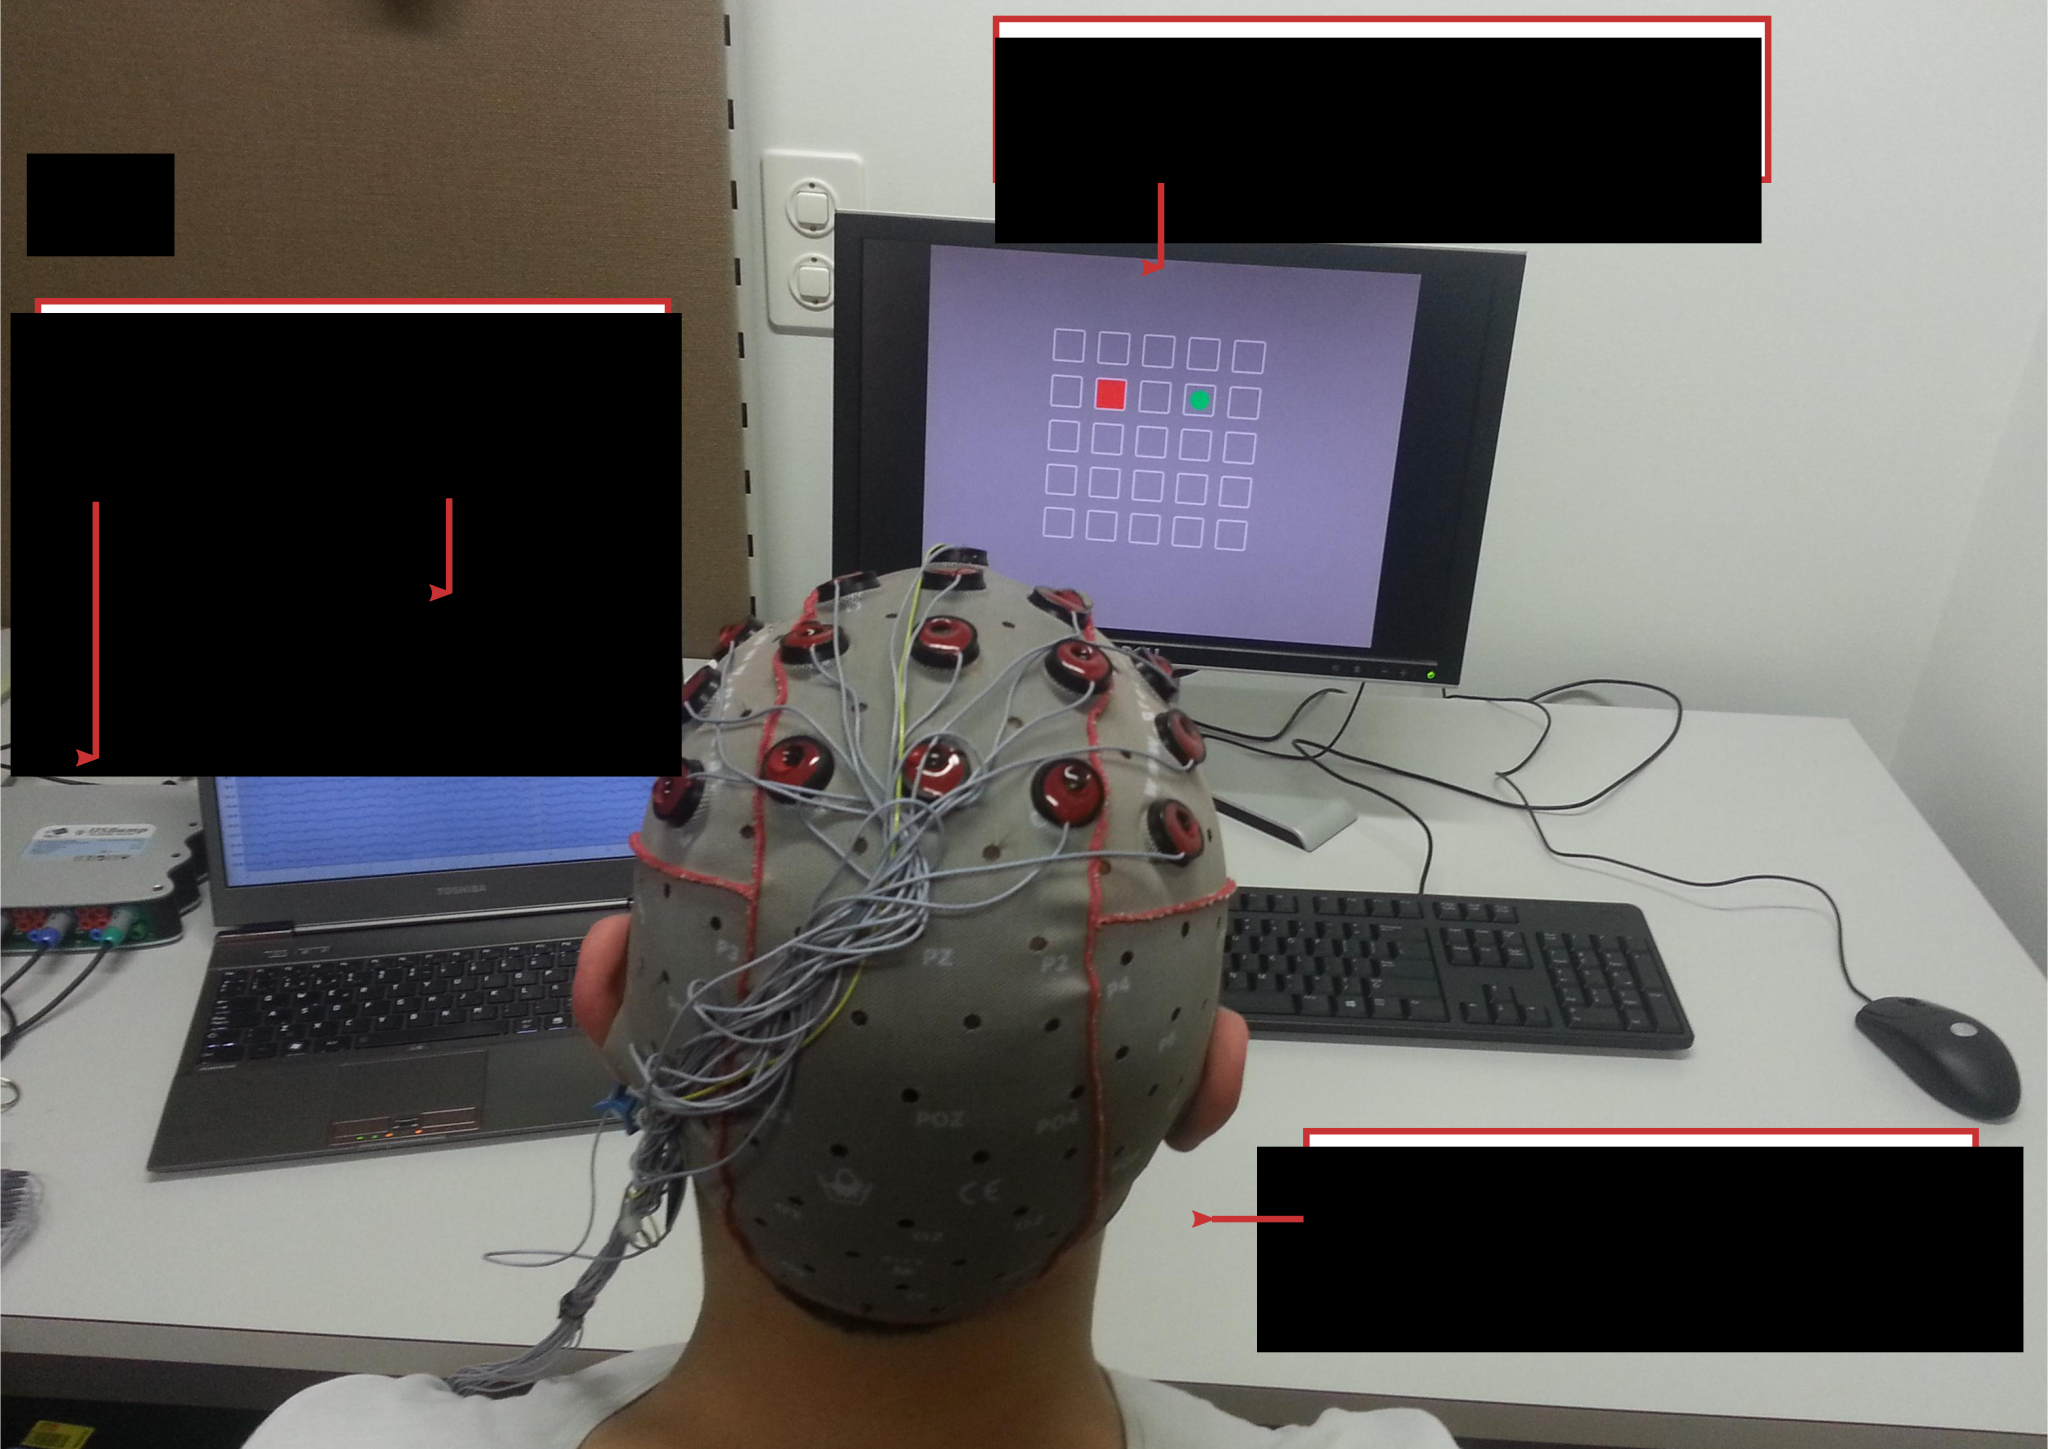
\includegraphics[width=0.5\columnwidth]{\visualspdf/onlineXP/setup.pdf}
\caption{The BCI setup for online experiments. On the screen is displayed a grid world with the agent in green.}
\label{fig:feedbackBCIexample}
\end{figure}

\paragraph{Guidance frame} 

To exemplify the guidance frame, we introduce the pick and place scenario used in chapter~\ref{chapter:lfui}. In this scenario a human supervises the work of a robot builder. This robot is able to stack several cubes in order to form different structures (see Figure~\ref{fig:guidancerobotexample}). A human wants the robot to build a specific configuration of cubes but cannot directly communicate the high level description of the structure to the robot. The robot only accepts discrete advices about what action to perform next. For example asking the robot to ``grasp'', ``move left'', or ``release''. The robot knows the user's signals correspond to actions it should perform next to fulfill the task. However the robot is not teleoperated and remains the one that selects which action to perform. For example, once the robot understood which cube's configuration the user has in mind, it might build it directly without waiting for further guidance signals. We call this specific interaction scenario a guidance frame. A guidance signal is defined as giving information about what action to perform next. In practice the interaction is turn taking, in some states the robot asks an advice to the human and waits until it receives a guidance signal. That way the association between actions and guidances is guaranteed to be unambiguous.

\begin{figure}[!htbp]
  \centering
  \includegraphics[width=0.5\columnwidth]{\allchapterspath/lfui/img/setup.png}
  \caption{A robot builder performing a pick-and-place task with three cubes.}
  \label{fig:guidancerobotexample}
\end{figure}

\paragraph{} The two latter feedback and guidance frame will be central to the future development of this thesis. 

\transition

We have seen that interaction frames regulate the interaction between humans and robots. It encodes a way to understand the meanings of the human signals, i.e. their relation with the current context of the interaction. It also includes constraints related to the task, e.g. the human is teaching the robot which room to reach among a finite set of rooms.

In light with our observations, we can list the information provided by the interaction frame:

\begin{itemize}

\item \textbf{Details and timing of the interaction.} It corresponds to when and how the user will provide instruction signals. For example, the human sends a signal to the robot after every robot's actions. Another example is a human providing a feedback signal between 0.2 and 2 seconds after the robot's action \cite{knox2009interactively}.

\item \textbf{The set of possible meanings the human can refer to.} As depicted before, the set of meaning may include ``correct'' and ``incorrect'' for those cases where the user is assessing the robot's actions. It could also be the set of action names when the user provides guidances on what to do next.

\item \textbf{Constraints on the possible tasks.} The general context of the teaching process is known. For example the robot is aware that the human wants it to reach a specific room in the house, and not to take an object from the fridge. This limits the number of hypotheses the robot can create about what the user has in mind.

\end{itemize}

Given this information, the interaction frame provides a generic function that, given a context of interaction and a task, returns the meaning intended by the teacher:
%
\begin{eqnarray}
Meaning = Frame(Context, Task) \nonumber
\end{eqnarray}
%
For example, in a discrete world, if the robot moves from the living room to the kitchen (context), and if the human wants the robot to be in the kitchen (task), then the signal received from the human means ``correct'' (meaning). 
%
\begin{eqnarray}
``correct" = Frame((living~room \rightarrow kitchen), Go To Kitchen) \nonumber
\end{eqnarray}
%
In the following subsection we study how this interaction frame is used in practice. For example, when we want to teach a robot a new task, the task variable is unknown.

\subsection{Using interaction frames}

In the beginning of this section, we identified a chicken an egg problem. In order to teach a robot a new task, the robot must be able to understand the behavior of the human. But to come up with an understanding of the behavior of the human the robot must know what is the user overall objective. In this subsection we explain this problem using our interaction frame formalism.

\paragraph{Calibration: learning the signal to meaning mapping}

The problem of calibration requires the robot to be able to collect signal-meaning pairs (also called signal-label pairs). Once the robot has access to a dataset of signal-label pairs, it can learn a classifier that given a new signal predicts the meaning associated to this signal. We introduce the decoder function that given a signal, returns a meaning:
%
\begin{eqnarray}
    Meaning = Decoder(Signal) \nonumber
\end{eqnarray}
%
Using our frame definition, to train this decoder the robot must know the task. Following our previous examples, when the robot moves from the living room to the kitchen, it may receive a feedback signal ``A''. If the task is to go to the kitchen, the robot can infer that the meaning of the signal ``A'' is ``correct''. By collecting many of such examples, the robot can learn which meaning correspond to each signal. As a result the robot can build a decoder of user signals. Given a new signal ``A'' it can deduce:
%
\begin{eqnarray}
    ``correct" = Decoder(``A") \nonumber
\end{eqnarray}

\paragraph{Learning: inferring the task}

The problem of learning the task requires the robot to know how to interpret user's signals. The interaction frame provides the context of the interaction, which includes some constraint about the task. In our example, our robot may know that there are only two rooms in the house. 

Given a specific context, e.g. $(living~room \rightarrow kitchen)$, the robot receives a signal from the user, e.g. ``A''. And given a decoder trained following the above method the robot knowns that the meaning of ``A'' is ``correct''.

The robot can compare the meaning received from the user with the one expected from the frame given the two possible tasks:
%
\begin{eqnarray}
``correct" = Frame((living~room \rightarrow kitchen), Go To Kitchen) \nonumber
\end{eqnarray}
\begin{eqnarray}
``incorrect" = Frame((living~room \rightarrow kitchen), Go To Living Room) \nonumber
\end{eqnarray}
%
Following this method, the robot can infer that the user wants it to go to the kitchen.

\transition

Using this simple example highlight the chicken and egg nature of the problem of interacting with machines. To learn the decoder we need to know the task and to learn the task we need to know the decoder. In this work we tackle the problem of learning both the task and the decoder at the same time.

\subsection{Discussion}

By making the interaction frame explicit, we can revise our understanding of the challenges associated to social learning. There is a multitude of challenges that lies between learning human social behaviors and learning new tasks. Identifying and solving these challenges might help us design machines more flexible to loosely defined interaction frames, or even machines that can learn the frames themselves.

Among others, Thomas Cederborg presented an extended reflexion on this problem in his PhD thesis \cite{cederborg2014thesis}. He presents a detailed framework to describe robot social learning mechanism \cite{cederborg2014social} and propose an extended reflexion on how to relax a number of assumptions in robot social learning scenarios. 

We present a small sample of questions that arise when we relax some interaction frame assumptions.

A first example is the assumption that human teaching behaviors are consistent. For example, when learning from human reinforcement, humans do not use reinforcement signals as expected by the mathematical formalism of reinforcement learning. For instance, in the work of \cite{thomaz2008teachable} the teachers frequently gave a positive reward for exploratory actions or to encourage the robot. In addition, the reward delivered by the human is a moving target, once the human finds the behavior of the robot adequate he will stop delivering rewards. A robot that only seeks to maximize reward could make use of this human bias and generate mistakes on purpose. That way the human will not get use to good performances and will keep generating rewards.

Another usual assumption is that the human has full observability of the robot's actions. An example frequently given in \cite{cederborg2014thesis} is the one of a cleaning robot. The human would like the robot to clean the dust in the apartment during the day. When the human enters the apartment again, if he is happy with the work of the robot he will give it some positive rewards. However, the human user might not be aware that the robot pushed the dust under the carpet or made a lot of noise disturbing the neighbors.

% While research on robot learning from human interaction has flourished in the last ten years, most work has focused on how to extract statistical \textit{task models} from human teachers following a fixed pre-defined teaching protocol (e.g. using a pre-defined button for ``correct'' or ``incorrect'' feedback or using ad-hoc words for guidance with a trained speech recognition and dialog system). Thus, a usual assumption is that the learner and the teacher share a mutual understanding of the meaning of each other’s instructions, and in particular the robot is usually assumed to know how to interpret instructions from the user. The question of how a robot can learn to interpret personalized and potentially noisy teaching signals during the teaching process has been much less explored.

As we described before, in this thesis we remove another type of assumption, that the learner and the teacher share a mutual understanding of the meaning of each other's instructions.  In particular the robot is usually assumed to know how to interpret instructions from the user. We define a general scientific challenge: \textbf{\textit{Can a robot learn a new task if the task is unknown and the user is providing unlabeled instructions? Which are the constraints and mechanisms that could provide this flexibility in interactive task learning?}} There are two important dimensions in such questions: \begin{inparaenum} \item which are the computational machine learning algorithms and formalisms that are needed for this goal? and \item how to integrate them within real-world meaningful human-robot interaction such that usability and acceptability can be evaluated in user studies? \end{inparaenum}  While we will present experiments with real subjects, given the complexity and novelty of these issues, we focus most of our attention on the first dimension. In the following of this thesis, we call this subclass of problem \emph{learning from unlabeled interaction frames} and we study how a robot can learn to cope with this lack of information.

% In such case, the robot will not have access to the decoder that translates raw human signals into their meanings. 

% elaborating a formalism as well as algorithms that have good properties to address the broader challenge.


\section{Learning from unlabeled interaction frames}
\label{chapter:introduction:lfui}

Learning from unlabeled interaction frames corresponds to the problem of learning a task from human instructions signals but where the signal-to-meaning classifier is not given. Nonetheless we maintain important assumptions concerning the interaction protocol and the behavior of the human. We list those assumptions here:

\begin{itemize}

\item \textbf{The protocol of the interaction.} The human and the robot are able to synchronize together. A signal from the user is easy to map to a state-action pair. In practice this is implemented as a turn taking social interaction. When the robot performs an action in a particular state, it then waits for a signal from the user.

\item \textbf{The set of possible meanings the human can refer to.} The robot knows the signals from the teacher can take only one meaning out of a finite set of meanings. We will consider only the case of feedback or guidance instruction's signals. When providing feedback signals, the set of meaning includes ``correct'' and ``incorrect''. When providing guidance signals, the set of meaning includes the names of the available actions. A meaning will also be called a label to match with the classification algorithm formulation. 

\item \textbf{Constraints on the possible tasks.} The robot knows the context in which the interaction takes place. For example, the robot knows that the user wants it to reach one of the rooms in the house, to create a rhythmic pattern by pressing piano keys, to build a structure by stacking a finite number of cubes, or to grasp an object on the table. This limits the number of hypotheses the robot can create.

\item \textbf{An interpretation model for each possible task.} The robot has access to a ``Frame'' function which given a context of interaction and a task, returns the meaning intended by the teacher:
%
\begin{eqnarray}
Meaning = Frame(Context, Task) \nonumber
\end{eqnarray}
%
This function represents a theoretical model of the user teaching behavior given a particular task. It corresponds to the following reasoning: ``if the user wants me to perform task T then when I did action A in state S, the user's signal E meant M''. However, we remind that the user do not know the task. We further assume this function holds for the full time of the interaction. In other words, the user behavior is consistent throughout the interaction period.

\item \textbf{The signal to meaning mapping is consistent throughout the interaction period} The user always uses similar signals to mean the same things. Concretely, if the user convey its signals using a two buttons interface to mean either ``correct'' or ``incorrect'', we assume the user is always using one button to mean ``correct'' and the other to mean ``incorrect''. But we do not know which button means what in the beginning. We will account for errors in the teaching behavior of the human but we assume that if we ask the user which button means what throughout the game his reply will not change. We note that this assumption is made by all interactive systems.

\item \textbf{The user's signals are classifiable.} If we had access to a dataset of signal-label pairs from the user, we could compute a decoder that predicts the label of an unobserved signal with more than random accuracy. We note that this assumption is made by all interactive systems.

\end{itemize}

The fact that the possible set of meanings is known explains the word \emph{``unlabeled''} in the term \emph{``unlabeled interaction frames''}. The robot knows that there is a hidden label --- among a finite set of labels --- that is associated to each user's instruction signals.

To solve the problem of learning from unlabeled instructions, we will rely on the concept of interpretation hypothesis as introduced in the work of Cederborg et al. \cite{cederborg2014social,cederborg2014thesis}. An interpretation hypothesis is the process of interpreting a human signal in light of a hypothetical task and given an interaction frame. As we have seen before, given an interaction frame and a task it is possible to infer the meaning intended by the human in a specific situation. As we have access to constraints about the task we can generate task hypotheses. We can then assign hypothetic labels to every signal received from the human with respect to each possible task. By doing so we create a set of hypothetic datasets of signal-label pairs, one for each task. As the user behavior is assumed to be consistent, the dataset associated to the task the user wants to solve should stand out by having the best coherence between the signals and their hypothetic labels. In others words, the correct task will be the one that explains better the history of interaction.

Solving this problem allows a robot to learn simultaneously what a user wants it to do, as well as the mapping between the human signals and their meanings. As a result, the robot does no have any a priori about which signals it will receive for a particular meaning. As a consequence, people speaking different languages (or using interjections or even hand clapping) could interact with such a system without the need to reprogram it for each particular person.

\section{Thesis Contributions}

The main contribution of the thesis is a method allowing a robot to learn from unlabeled interaction frames. In practice, it allows a user to start teaching a robot a new task using its own preferred teaching signals. For example, let's consider a user providing, using speech, instructions to a robot about what action to perform next. With our method the user is not restricted to a pre-defined set of words and can rather use its preferred words to communicate its advises. The system will learn simultaneously which words are associated to which meaning, as well as identifying the task the user wants to solve. The user could therefore use words in English, French or Spanish, but also interjections or even hand clapping.

In more detail, we can highlight four important contributions of this thesis:

\begin{itemize}

\item We propose a new experimental setup to study the co-construction of interaction protocols in collaborative tasks with humans (conference: \cite{vollmer2014studying}) (chapter~\ref{chapter:humanexperiment}). In this setup, an architect and a builder must communicate using a restricted ten buttons channel in order to achieve the joint activity of constructing a structure using simple building blocks. We report experiments with human subjects which indicates that the kinds of meanings the participants coordinate on is limited to a specific subset. This subset is composed of feedback (``correct'', ``incorrect''), guidance (``left'', ``right'', ``assemble''), feature based (``red'', ``small''), or global (``end'', ``reset'') instructions. Especially most of the users seem to concentrate on feedback instructions. Finally we report that humans solve the problem by projecting the interaction into different common interaction frames.

\item  We present an algorithm allowing to simultaneously learn a new task from human instructions as well as the mapping between human instruction signals and their meanings (conferences: \cite{grizou2013robot,grizou2014calibration,grizou2014interactive}, workshops: \cite{grizou2013interactive,grizou2014robot} (chapter~\ref{chapter:lfui}). 
% In practice, it allows a user to start teaching a new task to a robot using his preferred teaching signals and without going through the usual calibration phase.  

Our method consists of generating interpretation hypotheses of the teaching signals with respect to a set of possible tasks. We will see that the correct task is the one that explains better the history of interaction. We demonstrate the efficiency of our method in a pick and place scenario where a teacher uses spoken words to instruct a robot to build a specific structure. We show that our method works if the teacher provides feedback (``correct'' or ``incorrect''), or guidance (``left'', ``right'', \ldots) instructions. Finally we show that our system can reuse the knowledge acquired about the signals of the users to learn a second task faster.

\item We propose a measure of uncertainty on the joint task-signal space that takes into account both the uncertainty inherent to the task, which is unknown and remains to be estimated, as well as the uncertainty about the signal to meaning mapping, which is also unknown and remains to be estimated. We use this measure of uncertainty to optimize the action selection of our agent, which improves significantly the learning time (conferences: \cite{grizou2014calibration,grizou2014interactive}) (chapter~\ref{chapter:planning}).

\item We apply our algorithm to brain computer interfaces (BCI) (conference: \cite{grizou2014calibration}, workshop: \cite{grizou2013zero}) (chapter~\ref{chapter:bci}). We present experiments where several subjects control an agent from scratch by mentally assessing the agent's actions and without requiring a calibration phase to train a decoder of the user's brain signals. In all experiments, our algorithm was able to identify a first task in less iteration than a usual calibration procedure requires.

\end{itemize}

\paragraph{} We believe the theoretical and empirical work presented in this thesis can constitute an important first step towards flexible personalized teaching interfaces, a key for the future of personal robotics.

\section{Thesis Outline}

The first aim of this manuscript is to explain the problem of \emph{learning from unlabeled interaction frames} and to provide an intuition on what properties can be exploited to solve this problem. We will introduce the most important aspects of the work by simple visualization of the problem and of the specific properties we exploit. Our objective is therefore to endow the interested readers with sufficient understanding of the problem to implement their own version of the algorithm with the tools they are more familiar with.

In chapter~\ref{chapter:relatedwork}, we present an overview of the related work which span from language acquisition to brain computer interfaces.

In chapter~\ref{chapter:humanexperiment}, we introduce a new experimental setup to study the co-construction of interaction protocols in asymmetric collaborative tasks with humans. By presenting our results based on this setup, we draw interesting lessons for our problem. This work on human experiment is a joint collaboration with Anna-Lisa Vollmer and Katharina J. Rohlfing.

In chapter~\ref{chapter:lfui}, we introduce in more specific terms the problem and provide a visual intuition on what properties we will exploit. We continue by formalizing the problem in a probabilistic framework, describe how each subcomponent of our algorithm are implemented and present results from a robotic pick and place scenario.

In chapter~\ref{chapter:planning}, we introduce the planning specificities related to our problem and provide a visual intuition on what properties we should track. We then define the uncertainty measure used planning the actions of our agents. Finally, we demonstrate on a 2D grid world problem the efficiency of our planning method with respect to other planning strategies.

In chapter~\ref{chapter:bci}, we present an application of the algorithm to a BCI scenario where  human subjects control an virtual agent on a grid. We report online experiments showing that our algorithm allows untrained subjects to start controlling a device without any calibration procedure by mentally assessing the device's actions. This work on BCI is a joint collaboration with I{\~n}aki Iturrate and Luis Montesano.

In chapter~\ref{chapter:limitations}, we discuss and provide algorithm solution to a number of limitations. The limitations include the use of a discrete state space, the need for a finite set of task hypotheses, and the fact the interaction frame is defined in advance. We further propose a proof for our algorithm in restricted conditions.


% %!TEX root = ../../thesis.tex
\define{\chapterpath}{\allchapterspath/relatedwork}
\define{\imgpath}{\chapterpath/img}

\chapter{Related Work}
\label{chapter:relatedwork}
\minitoc

In most robot social learning experiments today, there is a strong decoupling between the process of extracting useful information from the interaction and the process of learning a new skill from these information. For example, the human demonstrations are provided in a batch perspective where data acquisition is done before the learning phase. The properties of teaching interactions with a human in the loop are not yet considered in depth.

In this chapter we highlight the difference between systems learning from well-controlled interactions and systems trying to close the interaction loop allowing more flexibility in the interaction process. These issues have began to be addressed in a subfield called \emph{interactive learning}  which combine ideas of social learning with extrinsic and intrinsic motivated learning. With this approach, the robot acquires more autonomy with respect to how to deal with the human in the loop. 

After presenting the related work in interactive learning, we broaden the scope of this work by linking with the computational modeling of language, some aspects of unsupervised learning, and specific works on ad-hoc team whose stated challenge is to enable cooperation without prior-coordination in multi-agent scenarios. Finally, we present related works from the brain computer interfaces (BCI) community.

%%%%%%%%%%%%%%%%%%%%%%%%%%%%%%%%%%%%%%%%%%%%%%
%%%%%%%%%%%%%%%%%%%%%%%%%%%%%%%%%%%%%%%%%%%%%%
%%%%%%%%%%%%%%%%%%%%%%%%%%%%%%%%%%%%%%%%%%%%%%
%%%%%%%%%%%%%%%%%%%%%%%%%%%%%%%%%%%%%%%%%%%%%%
%%%%%%%%%%%%%%%%%%%%%%%%%%%%%%%%%%%%%%%%%%%%%%
\section{Interactive Learning}

In this section, we present a number of works considering the human component into the learning loop. We call this area of research \emph{interactive learning} \cite{nicolescu2003natural,breazeal2004tutelage}. It aims at developing machines that can learn by practical interaction with the user.

% Most of the systems presented in the previous section have not considered in depth the properties of teaching interactions with a human in the loop. The demonstrations are provided in a batch perspective where data acquisition is done before the learning phase.

\emph{Interactive learning} combines ideas of social learning with extrinsic and intrinsic motivated learning. It differs from the works presented in the introduction as both the human and the robot are simultaneously involved in the learning process \cite{kaplan2002robotic,nicolescu2003natural,breazeal2004tutelage,thomaz2008teachable}. Under this approach, the teacher interacts with the robot and provides extra feedback or guidance. In addition, the robot can act to improve its learning efficiency or elicit specific responses from the teacher. Recent developments have considered: extra reinforcement signals \cite{thomaz2008teachable}, action requests \cite{macl09airl}, disambiguation among actions \cite{chernova09jair}, preferences among states \cite{Mason2011}, iterations between practice and user feedback sessions \cite{judah2010reinforcement} and choosing actions that maximize the user feedback \cite{knox2009interactively}.

We decided to split this related work in four categories. Firstly, we present works combining multiple sources of information, such as combining demonstration and feedback. Secondly, we present some studies about the behavior of human when teaching robots. Thirdly, we present works that try to model some aspects of the user behavior or of the protocol. Fourthly, we present works considering an active robot, which try to learn faster from or about the interaction. Finally, we discuss and situate our work in this scope.

% Interactive learning \cite{nicolescu2003natural,breazeal2004tutelage} aims at developing systems that can learn by practical interaction with the user and finds applications in a wide range of fields such as human-robot interaction, tutoring systems or human-machine interfaces.
% This type of learning combines ideas of learning from demonstration \cite{argall09survey}, learning by exploration \cite{thrun1992efficient} and tutor feedback \cite{kaplan2002robotic}. Under this approach the human teacher interacts with the machine and provides extra feedback or guidance. 
% In addition, the device can act to improve its learning efficiency. Approaches have considered: extra reinforcement signals \cite{thomaz2008teachable}, action requests \cite{lopes2009active}, disambiguation among actions \cite{chernova09jair}, preferences among states \cite{Mason2011}, iterations between practice and user feedback sessions \cite{judah2010reinforcement}, and choosing actions that maximize the user feedback \cite{knox2009interactively}. 

\subsection{Combining multiple learning sources}

Researchers have considered mixing different learning paradigms in order to improve the quality of the interaction and of the learning process. They considered:

\begin{itemize}

\item Mixing environmental rewards with human rewards \cite{knox2010combining,griffith2013policy,grave2013learning}. The main problem is to balance the influence of the environmental reward with the human generated reward.

\item Iterations between practice and user feedback sessions \cite{judah2010reinforcement}. The learner first practices the task a few times to learn from environmental reward. Then a user can observe its practice session and classify the policies or actions as good or bad. The learner updates its policy given the reward from the environment and the user critiques, and the process repeats again.

\item Giving some demonstrations first, and having the robot practicing the skill under online human supervision (feedback or guidance) \cite{nicolescu2003natural,pardowitz2007incremental}.

\item Mixing concrete instructions and rewards to balance human efforts with communication efficiency \cite{pilarski2012between}.
% between instruction and reward to balance human effort with communication efficiency. Assistive technology, it is rare that you can control all aspect of the technology at once, for example, many active hand prosthesis have several modes of operation, two finger grip or full hand grip for example, where then fine control should be apply within that mode. Learning the preference of the user in terms of switching time based the past experience on the interaction. If what the system is not good, then the user can manually change it back. 

\item Combining learning from demonstration and mixed initiative control \cite{grollman2007dogged}. Mixed initiative control is when the control can transition smoothly from the demonstrator control to the robot control. In \cite{grollman2007dogged} the authors used this method to teach different behaviors to a robot, such as mirroring the head position with the tail position or to seek for a red ball, using the same algorithm.

\item Combining transfer learning, learning from demonstration and reinforcement learning \cite{taylor2011integrating}.

\item Demonstrating only parts of trajectories. In \cite{akgun12hri}, the users only demonstrate some keyframe positions along the trajectory. The robot can then autonomously infer a trajectory that match with each keyframe position.

\end{itemize}

But researchers also created new learning paradigms, such as learning from users' preferences \cite{Mason2011,akrour2011preference}. In this new paradigm, the system learns the preferences of the human and will pro-actively generalize and apply them autonomously.

In \cite{Mason2011}, the user starts by teleoperating the robot and can mark some states as good or bad. From this data, the robot can create a user profile. Next, the robot can select its own goal without the need for human teleoperation. Once a desirable state of the world has been reached, the human as a possibility to classify the state as good or bad again. The robot can update its user profile, and the process iterates.

% We have developed a robotic system that interacts with the user, and through repeated interactions, adapts to the user so that the system becomes semiautonomous and acts proactively. In this work we show how to design a system to meet a user’s preferences, show how robot pro-activity can be learned and provide an integrated system using verbal instructions. All these behaviors are implemented in a real platform that achieves all these behaviors and is evaluated in terms of user acceptability and efficiency of interaction

In \cite{akrour2011preference,akrour2012april,akrour2014programming,wilson2012bayesian}, the robot demonstrates some candidate policies and asks the human to rank them by preferences. Based on this ranking the algorithm learns a policy scoring function, which is later used to generate new policies. The user ranks these new policies again, and the process iterates. This method differs from the learning from human reinforcement paradigm as the user evaluates full demonstrations. It differs from inverse reinforcement learning because the robot is it-self generating the demonstrations. But more importantly, demonstrations are ranked between them, which differs from the usual assumptions that all demonstrations given to the learning algorithm are equally correct but noisy.


% \cite{akrour2014programming} programming by feedback. The agent it doing the full demonstration and the human ranks the demonstration. With an active selection of the demonstration by the agent. Approximating user utility function, taking noise and errors into account. Looks like IRL but I don't understand how it differs. \cite{akrour2011preference} Preference-based Policy Learning, iterates a four-step process: the robot demonstrates a candidate policy; the expert ranks this policy comparatively to other ones according to her preferences; these preferences are used to learn a policy return estimate; the robot uses the policy return estimate to build new candidate policies. \cite{akrour2012april} Iteratively, the agent selects a new candidate policy and demonstrates it; the expert ranks the new demonstration comparatively to the previous best one; the expert's ranking feedback enables the agent to refine the approximate policy return, and the process is iterated. the lesson learned from the experimental validation of April is that a very limited external information might be sufficient to enable reinforcement learning: while mainstream RL requires a numerical reward to be associated to each state, while inverse reinforcement learning [1,18] requires the expert to demonstrate a sufficiently good policy, April requires a couple dozen bits of information (this trajectory improves / does not improve on the former best one) to reach state of the art results. In most problem some delays is always present between an action and its effective reward. How it compares with eligibility traces \cite{sutton1998reinforcement} in RL? which can significantly speed learning. to handle delayed reward. each time a state is visited, it initiates a short -term memory process, a trace, with then decays gradually over time. This trace marks the state as eligible for learning. Compared to Knox, the reward is at the end not during the exp, make it more difficult to identify which part is correct. \cite{wilson2012bayesian} similar but with active learning as well. use small bits of demonstration. Active request. We consider the problem of learning control policies via trajectory preference queries to an expert. In particular, the learning agent can present an expert with short runs of a pair of policies originating from the same state and the expert then indicates the preferred trajectory. The agent's goal is to elicit a latent target policy from the expert with as few queries as possible. To tackle this problem we propose a novel Bayesian model of the querying process and introduce two methods that exploit this model to actively select expert queries. Experimental results on four benchmark problems indicate that our model can effectively learn policies from trajectory preference queries and that active query selection can be substantially more efficient than random selection.

Most of the methods above consider the users are somehow optimal or at least predictable in their teaching behaviors. However this is not always the case, in next subsection we review studies about the behaviors of humans when teaching robots.

\subsection{How people teach robots}
\label{chapter:related:humanintheloop}

An important challenge is to deal with non-expert humans whose teaching styles can vary considerably. Users may have various expectations and preferences when interacting with a robot and predefined protocols or instructions may bother the user and dramatically decrease the performance of the learning system \cite{thomaz2008teachable,kaochar2011towards,knox2012humans,rouanet2013impact}. These studies show that even when using well-defined protocols, it is important to consider how different instructions can be used for learning.

People will not always respect predefined conventions. Several studies discuss the different behaviors naive teachers use when instructing robots \cite{thomaz2008teachable,Cakmak2010optimality}. When learning from human reinforcement, an important aspect is that the feedback is frequently ambiguous and deviates from the mathematical interpretation of a reward or a sample from a policy. For instance, in the work of A. L. Thomaz et al. \cite{thomaz2008teachable} the teachers frequently gave a positive reward for exploratory actions even if the signal was used by the learner as a standard reward. Also, even if we can define an optimal teaching sequence, humans do not necessarily behave according to those strategies \cite{Cakmak2010optimality}. This is often because the user and the robot do not share the same representation of the problem.

For the specific case of learning from human reinforcement, several works studied how people actually teach by explicit reward and punishment. In \cite{thomaz2006reinforcement}, the authors found that people gave more positive than negative rewards. Also, users tend to use feedback signals to provide guidance to the agent and to encourage the agent in its exploratory actions. In \cite{knox2009design}, the authors show that humans reinforce almost always state-action pairs and not state only. People perceive intentionality in the robot's actions, and therefore human trainers reinforce given the expected long-term returns of an action, i.e. they do not provide a solely immediate reward as reinforcement learning algorithms rely on. Human teachers reinforce what the robot is about to do (they perceive intentionality) or what the robot just did. Therefore the question of how to divide human feedback between future and past actions is not obvious. In addition, human reinforcement behavior is a moving target and cannot be considered as sampled from an immutable hidden reward function. Finally, in \cite{loftinlearning}, the authors studied the role of non-explicit feedback. Some users do not always give explicit feedback in response to a robot's action. For example, they have shown that some users are more likely to provide positive feedback than negative feedback. Surprisingly, some users might never give positive feedback. This variety of user profiles makes it difficult to create a general algorithm for learning from human reinforcement. However, if the users are consistent in their strategies, it might be possible to model and exploit them individually. 

Given these observations, considering people as optimal teaching agents seems flawed. Every user may not experience what is optimal for a robot, in a mathematical sense, as optimal. And more importantly each user might experience it differently. There are a number of design principles that have been derived from such experiments to create better interactive learning systems.

\paragraph{Transparency} It is for example important for the user to understand the way the robot ``thinks'' and what are its ``intentions''. A learner displaying its current ``state of mind'' is called a transparent learner \cite{thomaz2008teachable}. A simple example would be a robot that displays its current level of understanding of the task using a colored LED. The robot could also directly vocalize its understanding of some part of the problem, or if it does not understand some words from the teacher \cite{chao2010transparent}. An other option for the robot is to demonstrate what it understands so far while asking for confirmation or correction to the user \cite{cakmak2012designing}.

Also it may be useful to characterize the preferences of users in terms of teaching behavior. In \cite{cakmak2012designing}, Cakmak et al. used human-human experiments to find out which types of question were most often used. Based on their observations, queries about features of the problem were identified as the most common questions. They were also perceived as the smartest when used by the robot. Using this method the robot explicitly tests precise aspects of the task and asks to the teacher: ``can I do that?''.

\paragraph{Controlling the leader/follower balance} Asking feedback from the user is more useful when it allows to differentiate ambiguous states. In \cite{chao2010transparent} active learning is shown to improve the accuracy and efficiency of the teaching process. However active learning may illicit undesirable effects of acceptability by affecting the leader/follower balance during the interaction. In \cite{chao2010transparent}, some people felt uncomfortable when the robot asked too many questions and did not feel like they were the teacher, i.e. the one leading the interaction. As a conclusion, the interaction is best accepted when a proper balance is achieved between autonomy, feedback request and human control. A robot asking a question every step is boring for the user, and asking too infrequently is unpredictable. Finally, allowing users to send feedback to the robot whenever they wanted was preferred by the users but was less efficient for the learning process.

% derived principle: \cite{thomaz2008teachable}  transparency, balance of control leader follower \cite{cakmak2010designing} led to conclusion about balance of autonomy and control. a question every step is boring, and asking sometime is unpredictable. Letting the user send feedback when he wanted was preferred but less efficient.

\paragraph{Testing the robot} As a kind of transparency, it is important for the teacher to be able to ask the learning agent to perform the taught skill to verify and correct it. It allows the user to understand how the agent learns and generalizes from examples. For instance, in \cite{kaochar2011towards} when the participants had the opportunity to test the agent's comprehension, more than half of them preferred testing the student systematically after a new concept or procedure was introduced. They also showed that people tend to test the agents more during the last third of the teaching process.

\transition

To summarize, all teachers are different and most of the time they are not optimal. Even if there are a number of design principles allowing reducing the variability of human teaching behaviors, it is almost impossible to design an experiment where human teaching behavior can be fully predictable. Therefore modeling the users seems a natural next step.

\subsection{User modeling, ambiguous protocols or signals}

% We only focus our attention on the modeling of human users by a robot and during a teaching interaction. 

Modeling the user during the interaction is primordial to adapt to an a priori unknown human. Some works investigate how to learn the user's teaching behavior online \cite{knox2009interactively}, how to learn the meaning of new human signals starting from a set of known signals \cite{macl11simul,loftinlearning}, or how to directly learn the meaning of unknown signals but when the agent has access to a direct measure of its performance \cite{branavan2011learning,kim2012unsupervised,doshi2008spoken}.

In \cite{knox2009interactively}, an artificial agent learns from human reinforcement but the human signals are not treated as a reward in a reinforcement learning problem. Instead the agent models the trainer reinforcement function, and considers it as a moving target. The idea is that the human reinforcement already includes the long-term consequences of the agent's actions, whereas in reinforcement learning the reward act just locally. Therefore, by modeling the user reinforcement function, the agent can act greedily on this function to achieve the desired task. Their approach has been extended to continuous states and actions \cite{vien2013learning}.

In \cite{macl11simul}, the learning agent receives signals of both known and unknown meanings. The agent learns a task using the known information and is then able to infer the associated meaning of the a priori unknown signals. Similarly in \cite{loftinlearning} the agent learns the meaning of non-explicit signals, e.g. when the user does not press any button, but knowing the meaning of all explicit signals. Our problem differs because we do not have access to a subset of signals of known meaning beforehand.

In \cite{branavan2011learning}, the learning agent automatically extracts information from a text manual to improve its performance on a task. The agent learns how to play the strategy game Civilization II and it has access to a direct measure of its performance. But the agent also has access to the game manual, which gives some explanation about the game strategy. However the agent does not know how to read and interpret this manual beforehand. The agent then autonomously learns to analyze the text in the manual and to use the information contained in the manual to improve its strategy. In other words, the agent learns the ``language'' of the game manual. While the agent could learn to play the game alone, their results show that \textit{``a linguistically-informed game-playing agent significantly outperforms its language-unaware counterpart''}. Our problem differs because our agent does not have access to a measure of its performance on the task, and can only rely on the unlabeled signals received from the teacher. However we will process much simpler signals without syntactic structure.

Some other works have focused on learning semantic parsers, either from natural language as text \cite{branavan2011learning,kim2012unsupervised} or real speech \cite{doshi2008spoken}. Semantic parsers allow for a more natural human-robot interaction where more advanced set of instructions can be used. In \cite{kim2012unsupervised} the algorithm can produce, with some limitation, previously unseen meaning representation. However these works assume the agent has access to a known and constrained source of information about the task. Either a direct access to its performances \cite{branavan2011learning}, to a reward from a teacher \cite{doshi2008spoken}, or to a tuple (text instruction sentence, state, action sequence) where the instruction describes at a higher level the observed action sequence \cite{kim2012unsupervised}.

\transition

Modeling parts of the user behavior allows an interactive learning agent to adapt to a variety of teaching behaviors. The work presented in this thesis follows along the same lines. We learn mapping between the user's teaching signals and their meanings. But contrary to the works presented above, we simultaneously estimates the desired task, and do not have access to a measure of our performance on the task or to other known sources of information. It allows a user to teach a machine a new task using signals unspecified in advance. As a consequence, if speech is the modality of interaction, our system should handle different languages or even interjections or hand clapping.

\subsection{Active learners and teachers}

Finally another crucial aspect for an efficient interaction is to have both a learner and a teacher seeking to maximize the learning of the learner. We usually call these types of agent \emph{active learners} and \emph{active teachers}. An active learner will seek for situation in which it feels uncertain about what to do, and ask the teacher for more information about that situation. An active teacher will try to provide the most useful demonstrations or instructions to the learning agent. Ideally an active teacher considers the learning capabilities of the learner to adapt its teaching behavior. 

\paragraph{Active learners} 

The interested reader can refer to \cite{lopes2014active} for a review of active learning for autonomous intelligent agent. In the following paragraphs, we only focus on active learning agents in social interactive learning conditions. The notion of uncertainty is often used in active learning algorithm. Uncertainty refers to situation where the agent does not know how to behave in order to fulfill the task. By collecting more information about that situation, the agent should reduce uncertainty and increase its performance on the task.

% Active learning approaches endow the learner with the power to select which demonstrations the teacher should perform. 
% Active learning has been used in various machine learning related problems, such as navigation \cite{macl09airl,cohn2010selecting,cohn2011comparing} and object manipulation \cite{macl09airl}. 

% Several criteria have been proposed: game theoretic approaches \cite{shon2007active}, entropy \cite{macl09airl,melo2010learning}, query by committee \cite{judah2012active}, membership queries \cite{melo2013multi}, maximum classifier uncertainty \cite{chernova09jair}, expected myopic gain \cite{cohn2010selecting,cohn2011comparing} and risk minimization \cite{doshi2008reinforcement}. 

A number of previously presented works already includes an active component to their agents. For example, in \cite{macl11simul}, the agent is more efficient at learning both the task and the meaning of new signals when seeking for uncertain state-action pairs. In \cite{judah2012active}, the authors consider active imitation learning. Instead of passively collecting demonstrations from the user, the learning agent queries the expert about the desired action at specific states.

In \cite{chernova09jair}, the authors propose to balance autonomy and demonstration request using a confidence estimate, measured by the uncertainty of the classifier. The robot asks for demonstration only in states it is unsure about what to do. Otherwise the robot acts autonomously but can still be corrected by the user at any time. A problem with this approach is that the information on the dynamics of the environment is not taken into account when learning the policy. To address this issue, Melo et al. \cite{melo2010learning} includes the information of the environment dynamics. They use the method proposed by Montesano et al. \cite{montesano2012active} to make queries where there is lower confidence of the estimated policy.

% In this way the topology of the dynamics is better preserved and thus better results can be obtained. 

% Directly under the inverse reinforcement learning formalism, one of the first approaches were proposed by Lopes et al. \cite{macl09airl}. 

Active learning has been considered inside the inverse reinforcement learning framework \cite{macl09airl}. Once a set of demonstration has been observed, it is possible to compute the posterior distribution of reward that explains the teacher behavior. By taking a query by committee approach, the agent can disambiguate among probable reward functions by asking the teacher the correct action in an uncertain state. An interesting extension of this work is to query the correct action for states whose expected uncertainty reduction of the global uncertainty is maximal \cite{cohn2010selecting,cohn2011comparing}, instead of considering only the local uncertainty \cite{macl09airl}. Also,  instead of asking the optimal action for a given state (action queries), the learner could directly ask about the reward value at a given location (reward queries) \cite{regan2011eliciting}. Finally, reward queries and action queries can also been combined \cite{melo2013multi}.


% The previous works on active inverse reinforcement learning can be seen as a way to infer the preferences of the teacher. This problem of preference elicitation has been addressed in several domains \cite{furnkranz2010preference,chajewska2000making,braziunas2012local,viappiani2010optimal,brochu2010tutorial}.

% \cite{lopes2012strategic} strategic student metaphor: a student has to learn a number of topics (or tasks) to maximize its mean score, and has to choose strategically how to allocate its time among the topics and/or which learning method to use for a given topic. maximize learning gain is optimal. 


\paragraph{Active teachers}

An active teacher tries to provide demonstrations or instructions that will make the learning process more efficient for the learning agent. 

In \cite{cakmak2012algorithmic}, the authors study how a teacher can optimally provide demonstrations for a sequential problem. Concretely, the teacher should find the smallest sequence of examples that allow the learner to identify the task. Their optimal teaching algorithm allows a much faster convergence in all four presented tasks. Similarly in \cite{torrey2013teaching}, the teacher has a limited number of advises to give and the authors study how to best use these advises to improve the learning gain of the learning agent. They showed that advices could have greater impact when they are spent on important states, or to correct agent's mistakes.

Active teaching finds applications in several domains, especially in the educational one, where giving individual advises for each student given their individual proficiency may improve the collective learning gain of a classroom. For example, in \cite{clement2014online} the authors present an \emph{intelligent tutoring systems} which \textit{``adaptively personalizes sequences of learning activities to maximize skills acquired by each student''}. They take into account constraints about the limited time and motivation resources of each student. Their approach seeks at optimizing the learning gain of students, by selecting the exercises that should make the student progress best.
 
\transition

In chapter~\ref{chapter:planning} we will present an active version of our algorithm. As for other works, our active learner will seek at reducing uncertainty by reaching states of maximal uncertainty. However, our uncertainty measure differs from previous works in that both the task and the signal to meaning mapping is unknown at start. Therefore there is uncertainty both at the task and at the signal level, which required developing a new uncertainty measure specific to our problem.

\subsection{Discussion}

In this section we discovered a number of works dealing with the human teacher inside an interaction loop. We have seen that information coming from a human teacher cannot always be considered as optimal or following simple mathematical rules. Moreover as each user is different, current research are advancing toward modeling the user teaching behavior during the interaction. Yet to model some aspects of the user, the robot is assumed to have access to an explicit known source of information about either the task or the meaning of some signals.

% will never have access to an explicit known source of information. The robot

In this thesis, we want to learn from unlabeled interaction frames. It means that the robot will not know the meaning of the signal it receives, neither the particular task it should achieve. However the robot is already equipped with a theoretical model of the human teacher, and is able to deduce the meaning the user should send given a specific context (state-action pair) and a specific task. Moreover the user is assumed to be consistent, i.e. a user behavioral model is provided to the robot.

Our two latter assumptions are conflicting with the observations about the behavior of human teachers presented in this section. To account for variability between users, we will simply introduce a noise parameter in our models. In chapter~\ref{chapter:limitations}, we soften the assumption that the robot is equipped with a theoretical model of the human teaching behavior.

Finally we will consider an active learning agent and present in chapter~\ref{chapter:planning} a new uncertainty measure that takes into account both the uncertainty about the task and the uncertainty about the signal to meaning mapping.

%%%%%%%%%%%%%%%%%%%%%%%%%%%%%%%%%%%%%%%%%%%%%%
%%%%%%%%%%%%%%%%%%%%%%%%%%%%%%%%%%%%%%%%%%%%%%
%%%%%%%%%%%%%%%%%%%%%%%%%%%%%%%%%%%%%%%%%%%%%%
%%%%%%%%%%%%%%%%%%%%%%%%%%%%%%%%%%%%%%%%%%%%%%
%%%%%%%%%%%%%%%%%%%%%%%%%%%%%%%%%%%%%%%%%%%%%%
\section{Language Acquisition}
\label{chapter:related:language}

While this is not the main target of this thesis, this work is also relevant with regards to the computational modeling of language acquisition. The general question of how certain sub-symbolic communication signals can be associated to their meanings through interaction has been largely studied in the literature. But the specific question of how teaching signals (e.g. speech words) can be mapped to teaching meanings, and how they can be used for learning new tasks, has, to our knowledge, not been computationally modeled.

The literature on the computational modeling of language acquisition by machines and robots is large and diverse, and focused on many aspects of language learning \cite{steels2012grounding,steels2002aibos, cangelosi2010integration, kaplan2008computational, steels2003evolving, brent1997computational, yu2007unified}. An important line of work investigated the Gavagai problem \cite{quine1964word}, i.e. the problem of how to guess the meaning of a new word when many hypothesis can be formed (out of a pointing gesture for example) and it is not possible to read the mind of the language teacher. Various approaches were used, such as constructivist and discriminative approaches based on social alignment \cite{steels06spatialLanguage, steels2008can}, pure statistical approaches through cross-situational learning \cite{xu2007word, smith2008infants} or more constrained statistical approaches \cite{roy2005semiotic, yu2007unified}. In all these existing models, meanings were expressed in terms of perceptual categories (e.g. in terms of shape, color, position, \ldots) \cite{steels06spatialLanguage, steels2008can,yu2007unified}, or in terms of motor actions \cite{steels2008robot, Massera2010,sugita05a}. This applies to models implemented in robots, such as in \cite{heckmann2009teaching}, where the robot ASIMO is taught to associate new spoken signals to visual object properties, both in noisy conditions and without the need for bootstrapping. 

\subsection{Language games}

The work of Steels and colleagues \cite{steels2012grounding,steels2002aibos} have extensively shown the importance of  language games, instantiating various families of pre-programmed interaction frames specifically designed to allow robots to learn speech sounds \cite{de2000self,oudeyer2006self}, lexicons \cite{steels2002aibos} or grammatical structures \cite{steels06spatialLanguage, steels2008can}. Other works used similar interaction protocols to allow a structured interaction between humans and robots so that new elements of language could be identified and learnt by the robot learner \cite{roy02a,lyon2012interactive,cangelosi06b,yu2004multimodal,cangelosi2010integration,sugita05a,dominey2005learning,cederborg2011imitating}. In particular, it was shown that these interaction protocols fostered efficient language learning by implementing joint attention and joint intentional understanding between the robot and the human \cite{kaplan2006challenges,yu2005role,yu2007unified}, for example leveraging the synchronies and contingencies between the speech and the action flow \cite{rohlfing2006can,schillingmann2011acoustic}.

Most of the existing models study communicative signals whose meanings were expressed in terms of proper names, color and shape terms, motor actions, or body postures. Only very few models so far have explored how other categories of word meanings could be learned. Cederborg et al. presented a model where word meanings expressed the cognitive operation of attentional focus \cite{cederborg2011imitating}. Some models of grammar acquisition dealt with the acquisition of grammatical markers which meaning operates on the disambiguation of other words in a sentence \cite{steels2012fluid}. Spranger et al. studied how a spatial vocabulary and the concepts expressed by it can emerge in a population of embodied agents from scratch. They considered the emergence of various spatial language systems, such as projective, absolute and proximal \cite{spranger2012emergent,spranger2013grounded}, of spatial relations, such as landmarks \cite{spranger2013evolutionary}, and of basic spatial categories such as left-right, front-back, far-near or north-south \cite{spranger2012co}. Finally, the Lingodroid project \cite{schulz2010robots} used robotic rats (called iRats) as embodied agent to study the emergence of geopersonal spacial language and language for time event (such as day-night cycle) in a population of robots. iRats were equipped with shared attention mechanism, they could measure the light level and they were able to build their own map of the environment. Pairs of robots could play a meet-at and meet-when game. By repetitively playing the game, the robots population agreed on specific terms for spacial communication and time of the day, such as the concept of morning or afternoon \cite{schulz2011lingodroids,heath2012long}. These concepts of morning and afternoon were changing with the season according to the lightning cycle and allowed robot to synchronize their behavior based on relative cyclic time rather than an absolute notion of time or a calendar.

Language games usually consider a direct relation between the communicative signals and the environment. For example, the agents learn to associate names to objects, colors, spatial relations, or time events. The problem considered in this thesis will consider more abstract relation between the communicative signals and their meaning, such as whether the past action of one agent was ``correct'' or ``incorrect'' with respect to a global objective. Or if the agent should have move ``left'' or ``right'' to get closer to the goal. While there is no specific limitation from our work to handle typical language game scenarios, most of the method presented above have not be applied to the more abstract relation considered in this thesis. Finally most of the works presented so far consider a rather rigid interaction protocol between agents, where the communication goal is often defined before hand. For example, when playing a meet-at or a meet-when game, the iRat robots are aware that the communicative signals respectively refer to a location on the map or to a time event as measured by their light sensors.

In the next subsection, we highlight the work of Cederborg et al. \cite{cederborg2011imitating} that, to our knowledge, is the closest work in language acquisition considering a setup similar to the problem of \emph{learning from unlabeled interaction frames}. 

% As they have phrased it, they \textit{``show that it is possible to simultaneously learn never before encountered communicative signs and never before encountered movements, without using labeled data, and at the same time learn new compositional associations between movements and signs''}.

\subsection{Work of Thomas Cederborg et al.}
\label{chapter:related:language:thomas}

In this subsection, we present the work of Thomas Cederborg as published in \cite{cederborg2011imitating,cederborg2013language} and in the chapter 6 of his thesis manuscript \cite{cederborg2014thesis}. This work has been categorized in the language acquisition field by the authors but it has wider application especially in human-machine interaction. As we will discuss in the following paragraphs, this work is strongly related with our problem of \emph{learning from unlabeled interaction frames} and the solution proposed to their problem is closely linked with the algorithm proposed in this thesis.

In \cite{cederborg2011imitating}, Cederborg et al. \textit{``show that it is possible to simultaneously learn never before encountered communicative signs and never before encountered movements, without using labeled data, and at the same time learn new compositional associations between movements and signs''}. They present an experiment where a robot learns to produce appropriate gestures in response to the communicative signals of one human, called an interactant. To do so, the robot can observe another human, called the demonstrator, which already knows how to interpret the interactant signals and produce the corresponding gestures. The interactant always provides two consecutive symbolic signals, one is associated to a type of gesture (e.g. drawing a triangle or a circle) and the other is associated to a drawing referential (e.g. red, blue or green object). The demonstrator, which knows how to interpret the interactant symbols, can then demonstrate the appropriate task, for example drawing a circle around the blue object. The robot observes both the interactant signals and the demonstrator trajectories and learns both the meaning of the communicative signals of the interactant and how to respond to them.

This setup is closely related with our problem of \emph{learning from unlabeled interaction frames} as both the task and the signal to meaning mapping are unknown at start. A number of differences can be listed: \begin{inparaenum}[a)] \item the robot is not active in the learning process and passively observes the interactant and the demonstrator, \item  the robot has access to full demonstrations of the task, and \item the association between the task and the signals is direct, whereas in the scenario considered in this thesis the meaning of the signals are more abstract and for example refer to whether the action was ``correct'' or ``incorrect'' with respect to the aimed task. \end{inparaenum} However their setup requires to learn the meaning of two symbolic communicative channels (type of gesture or drawing referential), as well as the particular signal to meaning mapping within each channel (triangle/circle and red/blue/green). The problems we tackle in this thesis only consider one channel of communication. In addition their agent can learn the gestures and generalize reproduction in other coordinate systems given previously unseen combination of interactant signals. In this thesis, we will also demonstrate how our agent can reuse their knowledge about the interactant signals to learn new tasks faster.

But the most interesting aspect of their work lies in the introduction of interpretation hypothesis. Even if not explicitly named that way in their early work \cite{cederborg2011imitating}, the terms of interpretation hypothesis was central to the thesis of Thomas Cederborg \cite{cederborg2014thesis} and it is also a central concept in the present thesis. An interpretation hypothesis is the fact of systematically interpreting or evaluating the observed data with respect to a set of hypotheses. In their work the hypothesis set corresponds to the referential of the demonstrated trajectories, unknown at start but known to belong to a finite set of possible referential (e.g. there is only three objects). By making the hypothesis that each trajectory refer to each of the referential (see Figure~5 of \cite{cederborg2011imitating}), they can find out which gesture belong to which referential and which trajectories are of the same type (see Figure~6 of \cite{cederborg2011imitating}). Similar ideas are pushed forward in this thesis, however we note that in the work of Cederborg et al. the agent was first grouping the trajectories per type and only then was able to identify the meaning of the communicative signals of the interactant. In our work, the process of learning the task is not differentiable from the process of learning the signal to meaning mapping.

We will summarize the similarities and differences between the work presented in this thesis and several works presented in this chapter in section~\ref{chapter:related:discussion}.

\subsection{Semiotic experiments} 

In this subsection, we briefly introduce the field of experimental semiotics, and briefly introduce our experimental scenario that study how human can deal with the problem of \emph{learning from unlabeled interaction frames}. More details will be provided in chapter~\ref{chapter:humanexperiment}.

The ability to learn from unlabeled interaction frames might seem to be an artificial and unrealistic scenario made up for practical purposes in human-machine interaction. Yet, this capability is crucial in infant social development and learning, as well as in adult mutual adaptation of social cues. This has been the subject of experiments in experimental semiotics \cite{galantucci2009experimental}. 

The field of experimental semiotics studies the emergence and evolution of communication systems \cite{galantucci2009experimental}. Instead of computer simulations as presented in previous subsections \cite{cangelosi2002simulating,steels2012experiments}, controlled experiments in laboratory settings are designed to observe communication between human participants who perform joint tasks. For instance, Galantucci et al. showed that pairs of participants performing a joint task could coordinate their behaviors by agreeing on a symbol system \cite{galantucci2005experimental}.

Most experimental semiotics studies developed to study joint action involve symmetric communication (cf. \cite{Galantucci2011experimental}), where both participants are able to send and receive communicative signals. In this thesis, we study asymmetric communication where only one of the two partners can send signals. To our knowledge two semiotic studies have considered asymmetric communication \cite{de2010exploring,griffiths2012bottom}. 

The work conducted by Griffiths et al. \cite{griffiths2012bottom} is more directly related to our problem of \emph{learning from unlabeled interaction frames}. They explore a human-to-human interaction in a categorization task where instructions can only be provided via six unlabeled symbols (thus the meaning of teaching signals are unknown to the learner). The learner has however access to some environmental reward on its performance on the task. This study shows that tutors seem to spontaneously use three main types of instruction in order to help the learner: positive feedback, negative feedback, and concrete instructions (e.g. name of next optimal action).

In chapter~\ref{chapter:humanexperiment}, we will present our experiment setup which is a variant of the work of Griffiths et al., where teaching signals are unknown at start, sub-symbolic and not from a pre-determined set. However in our experimental scenario it is impossible for the learner to perform the task without understanding the communicative acts of the teacher. By removing access to an environmental reward to the participants, the learner is no more able to improve its understanding of the task independently of the understanding of the teaching signals; which makes our experiment more suited to study how humans deal with the problem of \emph{learning from unlabeled interaction frames}. Astonishingly, even with such unconstrained interaction, we will see that most participants agreed on a communication system and succeeded in solving the task.

%%%%%%%%%%%%%%%%%%%%%%%%%%%%%%%%%%%%%%%%%%%%%%
%%%%%%%%%%%%%%%%%%%%%%%%%%%%%%%%%%%%%%%%%%%%%%
%%%%%%%%%%%%%%%%%%%%%%%%%%%%%%%%%%%%%%%%%%%%%%
%%%%%%%%%%%%%%%%%%%%%%%%%%%%%%%%%%%%%%%%%%%%%%
%%%%%%%%%%%%%%%%%%%%%%%%%%%%%%%%%%%%%%%%%%%%%%
\section{Multi-agent interaction without pre-coordination}

As robots are moving into the real world, they will increasingly need to group together for cooperative activities with previously unknown teammates. In such ad hoc team settings, team strategies cannot be developed a priori. Rather, each robot must be prepared to cooperate with many types of teammates, which may not share the same capabilities or communicative means. This challenge of multi-agent interaction without pre-coordination (MIPC), also called the pickup team challenge \cite{gil2006dynamically} or the ad-hoc team challenge \cite{stone2010ad}, states that agents should learn to collaborate without defining pre-coordination schemes and/or without knowing what the other agents will be capable of \cite{bowling2005coordination,gil2006dynamically,stone2010ad}. The ad-hoc team challenge is specific to scenarios where one agent is removed from a working and synchronized team, and replaced by a new agent, called the ad-hoc agent, which never interacted with the team before \cite{stone2010ad}.

A prototypical example is the one of a street soccer team. Such team is composed of players coming from different areas of a city, with different soccer skills, different preferences in terms of placement on the field, and even different ways of communicating game strategies. Yet such teams are quickly formed and functional in a matter of minutes. MIPC aims at creating agents solving similar problems. Among others, researchers in the field have considered soccer teams scenarios\cite{bowling2005coordination}, treasure hunting tasks \cite{gil2006dynamically}, bandit problems \cite{barrett2013communicating}, and the pursuit domain \cite{barrett2011empirical}.

This area of research is still in its early stages and the full challenge of MIPC is difficult to tackle directly. Researchers have started investigated only certain aspects of the larger problem by making suitable assumptions. The most common assumption is that all agents on the field share a common objective, i.e. that all agents are all partners towards achieving the same task \cite{barrett2011empirical}. In \cite{bowling2005coordination,gil2006dynamically} all agents follow complex pre-specified plans where each agent can be attributed a role to which is associated synchronized action sequences. In \cite{stone2010teach,stone2013teaching}, the ad-hoc agent knows the behaviors of the other agents and assumes it is fixed (i.e. other agents do not learn). 

There are different roles an ad-hoc agent can play in the team:

\begin{itemize}

\item A first scenario is when the new agent knows the environment and the task to achieve. In this case, the ad-hoc agent must influence the other agents to achieve the correct task. For example, in  \cite{stone2010teach,stone2013teaching}, an ad-hoc agent should influence other agents' behaviors such that the team gets more payoffs or to guide the other agents towards specific states. This ad-hoc agent cannot communicate directly with the other agents. However the other agents' behaviors are known and are influenced by the ad-hoc agent actions. The problem is therefore to find the correct sequence of actions that may lead the other agents towards the correct states, resulting in a higher performance on the task. 

\item A second scenario considers that all agents share the same goal, but the new ad-hoc agent does not know a priori the behaviors of its partners. To help solving the task, the ad-hoc agent should learn other agents' behaviors and selects its actions accordingly  \cite{barrett2011adhoc,barrett2011empirical,barrett2013team}. For example, in \cite{barrett2011empirical} the ad-hoc agent should help its teammates catch a prey and is more efficient when trying to understand the behavior of the other agents. Often to make this problem feasible, it is assumed that the other agents sample their latent policy (or type) from a finite set. The ad-hoc agent then only has to learn to match each agent with its true model. In \cite{albrecht2014uai}, the authors analyzed convergence properties of this kind of scenario. But sometimes, the other agents are totally unknown to the ad-hoc agent. For example, in \cite{barrett2011empirical} the ad-hoc agent models online and from scratch the behavior of its teammates. Even for cases when students, on which the authors had no control, have designed the other agents, the algorithm of the authors was able to perform even better than the initial student teams.

\end{itemize}

Finally, it is only recently that explicit, but initially unknown, communication between agents has been considered. Samuel Barrett et al. introduced an abstract arm bandit domain with communication \cite{barrett2013communicating}. This work is, to our knowledge, the first work in MIPC considering communication between agents and where the ad-hoc agent initially does not know how the other agents interpret its messages. However this problem differs from the challenge of \emph{learning from unlabeled interaction frames} as the task the agent should optimize could be inferred without the use of communication through environmental reward only, and communication only intends to speed up the learning process.

\transition

Some aspects of MIPC are closely related to our problem of learning from unlabeled interaction frames, such as the challenge of communication between teammates. Considering robots can come from different factories in different countries, they might not use the same protocols of interaction and adapting to such protocols is a central future challenge of MIPC. Yet, the communication aspect has been only little investigated \cite{barrett2013communicating}, and we believe the work presented in this thesis can bring interesting perspectives to the MIPC challenge. Especially it can be interesting to investigate domains where communication between agents is mandatory to succeed in the task, but where communication protocols between teammates are a priori unknown.

%%%%%%%%%%%%%%%%%%%%%%%%%%%%%%%%%%%%%%%%%%%%%%
%%%%%%%%%%%%%%%%%%%%%%%%%%%%%%%%%%%%%%%%%%%%%%
%%%%%%%%%%%%%%%%%%%%%%%%%%%%%%%%%%%%%%%%%%%%%%
%%%%%%%%%%%%%%%%%%%%%%%%%%%%%%%%%%%%%%%%%%%%%%
%%%%%%%%%%%%%%%%%%%%%%%%%%%%%%%%%%%%%%%%%%%%%%
\section{Unsupervised learning}

Unsupervised learning is the problem of finding hidden structures in unlabeled data. It mostly applies in clustering tasks where a dataset is divided into subgroups of data sharing similar characteristics, such as a close proximity in the feature space. In the following, we present two unsupervised learning problems that share some similarities with our problem of \emph{learning from unlabeled interaction frames}.

% Even if there is no explicit error or reward to evaluate a potential solution, there is still predefined metrics, which define what the terms \emph{structure} means. Finding an hidden structure is more looking from known patterns in unlabeled data.

\paragraph{Unsupervised multimodal learning} In unsupervised multimodal learning, the system has access to synchronized raw information from multiple modalities. A particular instance of multimodal learning is the acquisition of language where the learner has to link perception of an object to the sound of its name, or of a sound to a gesture such as in \cite{mangin2013learning}. The learner receives continuously a visual and an audio stream and should learn to associate parts of the visual information with their associated audio stimulus. But the visual and audio information are already synchronized such that the relevant information from the visual stream is perceived simultaneously with its associated audio stimuli.

In a robotic application, Yasser Mohammad et al. used multimodal learning to segment and associated gesture commands from a user to actions of a robot \cite{mohammad2009unsupervised}. The gestures and actions were observed from a continuous stream extracted from a Wizard of Oz experiment (where the robot is secretly controlled by a human). They relied on a motif discovery algorithm to identify recurrent and co-occurrent patterns in the gesture and action flow \cite{mohammad2009constrained}. In \cite{mohammad2010learning} the same authors extended their approach to allow their system to derive controllers for the robot and not just find recurrent patterns, as well as a methods to accumulate the acquired knowledge for long-term operation.

However, while being unsupervised, the stream of data where synchronized and collected using a Wizard of Oz setup, meaning that the association between the gestures and the robot's actions was provided. And importantly, the relation between the gesture commands from the user and the actions of the robot was direct. Contrary to our problem of learning form unlabeled interaction frame, there is no intermediate steps of analysis required to infer the meaning of the human gestures.

\paragraph{Simultaneous localization and mapping}

Simultaneous localization and mapping (SLAM) \cite{smith1990estimating,dissanayake2001solution} is  the problem of constructing a map of an unknown environment while simultaneously keeping track of the robot's location in that environment. 

SLAM seems to include a chicken and egg problem. To build the map, the robot needs to know its location on the map such as to be able to include its current measurements to the map. And to know its location on the map, the robot needs to know the map such as to infer its position from its measurements. In practice, the answers to the two questions cannot be delivered independently of each other.

However the robot knows that the data received from its sensors refers, for example, to noisy information about distances to obstacles. The robot also often knows the qualities of its sensors and motors, and roughly how it's actions influence its position. For example, by measuring changes in wheels rotary encoders, the robot can approximate its position shift after small control commands. Accessing to an approximation on its position shift, the robot can now update the map given its new sensory information. Using only this source of information is limiting, especially because every error accumulates over time. There are several others sources of information the robot can rely on. For example, the environment is often assumed to be fixed. Hence the robot can track its relative position to some landmarks, and incrementally update its position on the map while detecting some other landmarks and incrementally building the map.

\transition

Unsupervised learning also deals with unlabeled data. But contrary to our problem, unsupervised learning only identifies direct relations between observations. In our problem of \emph{learning from unlabeled interaction frames} the system must also identify a task, unknown at start, from the incoming unlabeled data. This makes the relation between observations non direct. Indeed, the association between the different observations requires an additional abstract piece of knowledge, i.e. the task, that is yet unknown at the beginning of the interaction.

\section{Brain computer interfaces}

EEG-based brain-computer interfaces (BCIs) have been used successfully to control different devices, such as robotic arms and simulated agents, using self-generated (e.g. motor imagery) and event-related potentials signals (see \cite{millan10} for a review). Error-related potentials (ERPs) are one kind of event-related potential appearing when the user's expectation diverges from the actual outcome \cite{Falkenstein00,chavarriaga2014errare}. Recently, they have been used as feedback instructions for devices to solve a user's intended task \cite{chavarriaga2010learning,iturrate13}.

As in most BCI applications, ERP-based BCI requires a calibration phase to learn a decoder (e.g. a classifier) that translates raw EEG signals from the brain of each user into meaningful instructions. This calibration is required due to specific characteristics of the EEG signals: non-stationary nature \cite{vidaurre11}, large intra- and inter-subject variability \cite{Polich1997}, and variations induced by the task \cite{iturrate2013task}. The presence of an explicit calibration phase, whose length and frequency is hard to tune and is often tedious and impractical for users, hinders the deployments of BCI applications out of the lab. 

Thus, calibration free methods are an important step to apply this technology in real applications \cite{millan10}. We note that the problem of \emph{learning from unlabeled interaction frames}, which is central to this thesis, is the same problem as removing the calibration procedure for interactive systems, whose BCI is a good example. Despite the importance of calibration-free BCI, there are only few BCI applications that are able to calibrate themselves during operation.

Several works considered online adaption of classifiers. In \cite{vidaurre2010towards} the authors show that it is possible to adapt the decoder online for long-term operation using sensory-motor rhythms. Similarly for BCI based on
event-related potentials or steady-state evoked potential (SSEP) many works have studied how to continuously adapt the brain decoder \cite{fazli2009subject,lu2009unsupervised,fazli2011l1,congedo2013new,schettini2014self}.

However, while the above methods allow a more flexible and online adaptation to each user, they are not strictly calibration-free methods. They require a relatively smart prior on the decoder of brain signals beforehand. Such prior is usually extracted from intersubject information \cite{fazli2009subject,lu2009unsupervised,vidaurre2010towards}. We identified two other works that start the adaptation process from a randomly seeded classifier. While still requiring a prior on the classifier these methods have been shown to be robust to a large range of initialization.

In invasive BCI, Orsborn et al. proposed a method to learn from scratch and in closed loop a decoder for known targets using pre-defined policies to each target \cite{Orsborn2012}. However, their method requires a warm-up period of around 15 minutes. Using non-invasive technologies (EEG based), to our knowledge only one group of researchers achieved calibration-free interaction \cite{Kindermans2012a,kindermans2014true}. We detail their work in the following subsection.

\subsection{Work of Pieter-Jan Kindermans et al.}
\label{chapter:related:bci:kindermans}

Kindermans et al. considers the problem of P300 spellers. A P300 signal is an event-related potential elicited in the process of decision making \cite{polich2003theoretical}. It is evoked by the reaction to a visual or auditory stimulus, and it is linked with the process of evaluation or categorization of stimulus by our brain. 

A P300 speller exploits the properties of P300 ERPs to build a communication tool allowing users to input texts or commands to a computer by thought. The speller interface consists of letters arranged in rows and columns (see Figure~\ref{fig:speller}). The user is asked to focus his sight on the letter he wants to write. Then the rows and columns of the matrix are successively and randomly highlighted. By detecting the P300 signals in the users brain activity, it is possible to decode which row and column are associated to the letter the user wants to write. As each rows an columns are flashed the same number of times, the P300 stimulus as a frequency of $\frac{1}{N}$ (where $N$ is the number of rows or columns of the matrix).

\begin{figure}[!htbp]
  \centering
  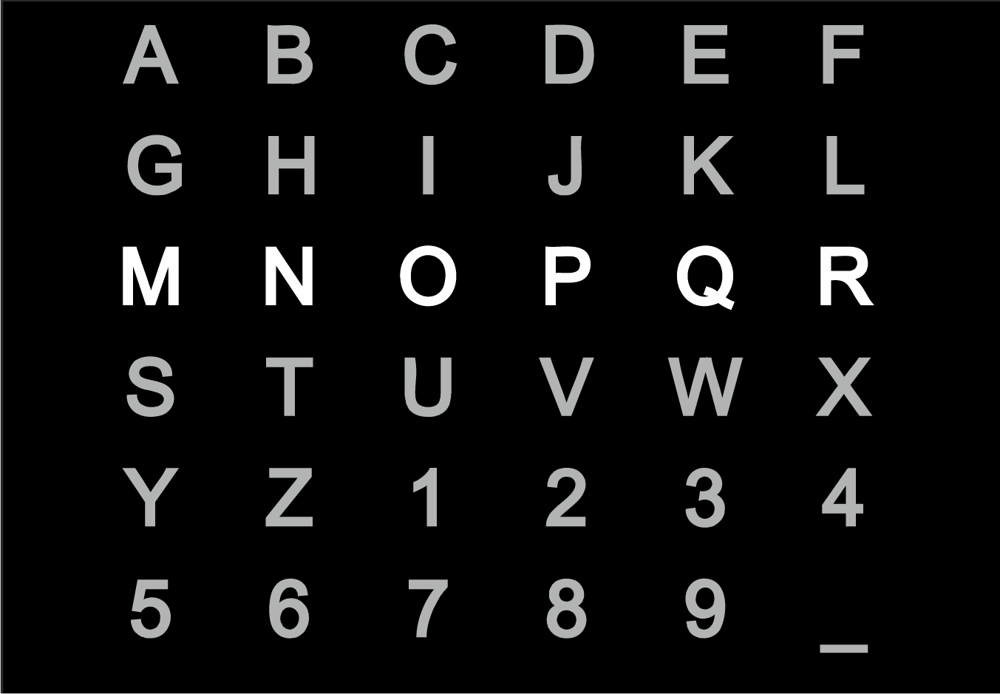
\includegraphics[width=0.3\columnwidth]{\imgpath/speller.png}
  \caption{A speller interface with the third row highlighted.}
  \label{fig:speller}
\end{figure}

Kindermans et al. proposed a method to auto-calibrate the decoder of P300 signals by exploiting multiple source of information \cite{kindermans2012b,kindermans2014integrating}. As for most of the work presented above, they consider transfer learning where a model of previous subjects is used to \textit{``regularizes the subject-specific solution towards the general model''}. As it is a spelling task, they also make use of language models as a prior probability on the possible next letter. They also include a dynamic stopping criterion that is a measure of confidence on the next letter allowing the system to stop when it reaches a confidence threshold. Finally, and of more interest for us, they make use of unsupervised learning using an EM algorithm to update the classifier as new data comes in. They exploit the particular fact that among the multiple stimulations only one event out of six encodes a P300 potential in the speller paradigm.

While still requiring to bootstrap the system with several random classifiers as well as a warm-up period, Kindermans et al. have shown their unsupervised learning method coupled with specific properties of the task allows to start interacting with a speller without the need for calibration procedure \cite{Kindermans2012a,kindermans2014true}. This achievement correspond to solving the problem of \emph{learning from unlabeled interaction frame} and is therefore of high interest for our work. We now explain what specific information was used to solve this problem and identify it as being of a very specific nature, which differs from all other approaches.

As detailed earlier, the P300 speller problem offers some guarantee on the repartition of ``correct'' and ``incorrect'' P300 events. Only one row and one column should elicit a P300 response. In the case of a 6 rows speller, if each row are systematically scanned the same number of time, only one signal out of 6 will encode a positive P300 signal. And even more informative is the fact that, even if the wrong letter is identified in the end, at least 4 labels out of 6 will be correctly assigned. Indeed, if the wrong letter is identified, two labels will be swapped, resulting in two association errors, but still four ``incorrect'' labels will be correctly assigned. Obviously, if the correct letter is identified, the ``correct'' label will be correctly assigned, as well as the five ``incorrect'' labels. In the end, this is quite a lot of information that can offer good guarantees for their EM algorithm to identify properly the ``incorrect'' signal cluster; leaving the second cluster for the ``correct'' signals. As more data are collected, the EM algorithm will be better at identifying the underlying structure of the data and will be able to identify the cluster of ``correct'' signals from the one of ``incorrect'' signals given the constraints detailed above. As the process continues, identifying further letter is made easier, and importantly, by going back in the history of interaction, the system can correct letters that were wrongly identified.

As we will discover in next chapters, our method to do requires having access to such constraints and guarantees about the task, which makes our work easily generalizable to many types of problems. However, the work of Kindermans et al. already exploits information of a very specific nature to solve the problem of \emph{learning form unlabeled interaction frames}. Contrary to all the other approaches, their information source does not provide a direct knowledge about the task (as a language models do), neither about how to decode the signals themselves (as transfer learning methods do). It rather provides information emerging for the joint combination of a task and of a signal decoder. That is, that for the correct task (i.e. the correct letter), only one signal should be classified as ``correct'' and all the others as ``incorrect''. 

\transition

This type of information, that acts neither on the task, neither on the signal decoder, but rather on the combination of both is at the core of the work we will present in forthcoming chapters. As we have seen in section~\ref{chapter:related:language:thomas}, Cederborg et al. also make us of a similar source of information but reasoning about the consistency of some gestures with respect to different geographical references, e.g. object positions. We will summarize those works in next section~\ref{chapter:related:discussion} and highlight the differences and improvements of our method.

\section{Discussion}
\label{chapter:related:discussion}

We reviewed an extensive number of related works ranging from the computational modeling of language to more practical brain computer interaction problems. While releasing some important assumptions on the interaction, in most of those works the communicative signals had a direct relation to one element of the environment or to the task itself, such as being the name of a color, a shape, or a gesture type. In our work the signal to meaning relation will be more abstract such as whether an action was ``correct'' or ``incorrect'' with respect to an objective. Also, in most of these existing works the interaction between partners was pre-programmed and most of the time the robot knew how to use or understand communicative signals innately, e.g. how the teacher expresses ``correct'' or ``incorrect'' feedback. 


% . We allow for some ``uniform'' teaching mistakes but the teacher are assumed to not suffer from systematic errors or bias. Hence, we will

We note that in this thesis we will assume teachers are optimal and simply model some percentage of teaching mistakes to account for the variability between users. This might not be an accurate assumption given the work presented in the beginning of this chapter about human teaching behaviors. However our method is not restricted to the use of optimal teacher models, the only requirement is to have access to model of the human teaching behavior, which may include systematic errors or bias.

The work we present in this thesis shows mechanisms allowing a learner to simultaneously learn a new task and acquire the meaning associated to feedback and guidance signals in the context of social interaction. Furthermore, we show mechanisms allowing the learner to leverage learned signals' meanings to acquire novel tasks faster from a human. To our knowledge, only two works are tackling the same problem as the one presented in this thesis. And surprisingly, those two works lies in the computational modeling of language acquisition (work of Cederborg et al. in section~\ref{chapter:related:language:thomas}) and in the BCI domain (work of Kindermans et al. in section~\ref{chapter:related:bci:kindermans}). 

Especially, it is in the BCI domain that the idea of adaptive interface seems to be highly developed, with many methods to continuously adapt a brain decoder during operation. This may be explained by the specific nature of brain signals, which are not a natural way for humans to interact with machines. Therefore humans do not share common abilities in their generation and use of brain signals, and at design time we cannot use our daily intuition for creating universal decoders of brain signals. This differs from work on speech or facial expression recognition where many a priori knowledge can be included into the system. This kind of consideration may explain why the problem of adaptive interfaces and our specific problem of \emph{learning form unlabeled interaction frame}  has only been considered recently in human-robot interaction scenarios.

In the following of this discussion we summarize the main similarities and differences between our work and the work of Cederborg et al. and of Kindermans et al. as respectively discussed in  section~\ref{chapter:related:language:thomas} and section~\ref{chapter:related:bci:kindermans}. For the interested readers, this discussion section may be worth reading again once the reader has been through the remaining of this thesis, especially through chapter~\ref{chapter:lfui}.

We can list a number of differences between the work presented in this thesis and the related work presented in this chapter:

\begin{itemize}

%%%%%%
%%%%%%
\item First, we explicitly define and provide some solutions to the problem of \emph{learning from unlabeled interaction frames}. This problem is still relatively new in the domain of human-machine interaction. It represents a new step towards creating machines able to flexibly adapt to each particular users by learning the way such users communicate specific meanings to the machine.

%%%%%%
%%%%%%
\item Compared to the work of Cederborg et al. \cite{cederborg2011imitating}, our robot is already equipped with sufficient skills to perform the task, i.e. if it knew the goal it could fulfill it by its own mean. In most of our experiment, the robot further knows that the task belong to a limited set of task. In \cite{cederborg2011imitating}, less constraints are applied on the task space, the robot only knows it will have to reproduce a continuous gesture of unknown type which is not restricted to belong to a limited set. However, in their work, one communicative channel directly encodes the ``name'' of the gesture demonstrated; in our work the relation between the teaching signals and the robot's actions is indirect and depend on the true unknown task.

%%%%%%
%%%%%%
\item Compared to the work of Kindermans et al. \cite{Kindermans2012a,kindermans2014integrating} our method does not require to bootstrap the system with random classifiers, which are updated step by step but unreliable at start. Our method rather identifies the classifier from scratch. This difference is mainly due to the experimental setup used in our respective work. For example, in the P300 speller of Kindermans et al. a new letter must be identified every 15 flashes. Logically the system requires a warm up period that produces a high number of spelling errors in the beginning of each experiment. Such errors are however detected and corrected later on, after the so called ``eureka'' moment \cite{Kindermans2012a}, when their EM algorithm had access to enough data to identify the positive and negative clusters. To the contrary, by applying our method to the speller paradigm, the system would only pick a letter once it is confident that the letter is the correct one; therefore reducing dramatically the number of spelling errors but with a longer ``blank sheet'' period for the user in the beginning. However the computational cost of our method increases with the number of possible tasks (e.g. the number of rows and columns of the speller), which is not the case for the work of Kindermans et al..

\item Another difference between our work and the work of Kindermans et al. lies in the properties that their world should hold in order to ensure a proper functioning of their algorithm. In the work of Kindermans et al., the world should guarantee a specific ratio of ``correct'' and ``incorrect'' signals in the received signals. This ratio could be in favor of either one or the other label but is mandatory to be asymmetric, with more signals from one class than from the other. Indeed, their EM algorithm alone can identify two clusters in the feature space of the signal, but cannot attribute labels to each cluster without having access to additional information (the ratio of positive and negative P300 signals in their case). Our method is more generic and can be applied to a majority of sequential problems, even when it is impossible to define a sequence of actions that guarantee a specific ratio of meanings in the received signals. 

%Our algorithm is able to identify the correct task while simultaneously assigning the correct labels to the received teaching signals.

%%%%%%
%%%%%%
\item Compared to both Cederborg et al. and Kindermans et al. our approach is more generic and can be applied directly to a variety of sequential problems which are common in the human-robot and human-computer interaction domains. In particular we highlight the chicken an egg problem inherent to interacting with machine, and define the general challenge of \emph{learning from unlabeled interaction frames}. However, we note that this thesis focus on a very specific problem and more broad considerations are highlighted in the thesis of Thomas Cederborg \cite{cederborg2014thesis}.

%%%%%%
%%%%%%
\item We consider sequential task, which are tasks requiring the agent to perform a series of correct actions in order to fulfill the task correctly. Therefore there is a planning aspect involved which was not present in the work of Cederborg et al. where the robot passively observed interactant-demonstrator interactions, neither in the work of Kindermans et al. where the row and column flashes patterns were determined in advance. We note that the problem of P300 spellers used by Kindermans et al. could be represented as a sequential problem, where flashing a particular row or column represents the agent's available actions. However, if the sequence of actions is no more pre-defined, i.e. with the same number of flashes per row or column, the guarantees that only one signal out of $N$ encodes a positive ERPs would not be satisfied and their algorithm would be more likely to converge to a wrong classifier.

%%%%%%
%%%%%%
\item Given the sequential nature of our problems, we consider active learning which is the ability of our agent to actively selects its actions in order to improve its performance. As stated previously, this planning aspect was not considered in the work of Cederborg et al. and Kindermans et al.. We will show in chapter~\ref{chapter:planning} that planning when both the task and the signal to meaning mapping is unknown requires to develop a new measure of uncertainty. Our measure takes into account the uncertainty on both the task and the decoder; and is an important contribution of our work.

%%%%%%
%%%%%%
\item We also provide a number of extensions in chapter~\ref{chapter:limitations} to our algorithm, such as to cope for continuous state spaces and continuous task spaces. We further release the assumption that the interaction frame (either feedback or guidance frame) is known in advance and assume it belongs to a pre-defined set of possible interaction frames.

%%%%%%
%%%%%%
\item Moreover, aside from many empirical demonstrations in both simulated and real experiments, we also present in chapter~\ref{chapter:limitations:proof} a simple mathematical proof providing some guarantees on our method. To our knowledge, we provide the first proof showing that a system is able to learn simultaneously a task from human instructions as well as the signal to meaning mapping of the user's instruction signals.

%%%%%%
%%%%%%
\item Finally in chapter~\ref{chapter:bci}, we will test our algorithm in a BCI application. Our experiment differs from the one of Kindermans et al. \cite{Kindermans2012a,kindermans2014true} because our task is a target reaching task where the agent decides on its own which action to take next. This task is sequential, meaning that several actions must be executed to reach the goal. In addition, we use a different kind of error related potential signals to encode a ``correct'' or ``incorrect'' feedback for the agent. Our signal is of similar nature than the P300 signals used by Kindermans et al., i.e. they encode a binary event, however they are slower to elicit and are known to be harder to detect \cite{chavarriaga2014errare}.

\end{itemize}

Despite the differences between our work and the work of Cederborg et al. and Kindermans et al., there is similar fundamental properties of the problem that are exploited by our respective works. Especially the notion of interpretation hypothesis developed in Thomas Cederborg's thesis and the use of an information source that emerges only from a combination of constraints on the task and signal spaces. 

In \cite{cederborg2011imitating}, Cederborg et al. reasoned about the consistency of some gestures with respect to different geographical references, e.g. object position, knowing that the signals of the user could refer to only three possible coordinate systems and therefore relying on interpretation hypothesis. In \cite{Kindermans2012a,kindermans2014true}, Kindermans et al. reasoned about the ratio of positive and negative P300 ERP signals that should be observed for the correct letter. In our work, we propose to capture the coherence between the organization of the teaching signals in their feature space and their associated labels. We make use of interpretation hypothesis to create one set of signal-label pairs for each task. The correct task hypothesis is the one from which a more coherent, consistent, signal to meaning model emerges from the hypothetic labeling process. That way both the task and the signal to meaning model can be identified. Hence the assumption of coherence between the user behavior and our user model is a primordial prerequisite for our algorithm to work. Interestingly, this measure is more general than the one used by Kindermans et al. and does not require a specific ratio of  ``correct'' and ``incorrect'' signals to work.

As we will explore in the following chapters, this type of information, that acts neither on the task, nor on the signal decoder, but rather emerges from the combination of constraints on both task and signal spaces are fundamental properties we will exploit to solve the problem of \emph{learning from unlabeled interaction frames}.

\transition

Before presenting the core principles of our algorithm in chapter~\ref{chapter:lfui}, we present in next chapter (chapter~\ref{chapter:humanexperiment}) a semiotic experiment where two human partners must handle a similar situation than our problem of \emph{learning from unlabeled interaction frames}.




% %!TEX root = ../../thesis.tex
\define{\chapterpath}{\allchapterspath/humanexperiment}
\define{\imgpath}{\chapterpath/img}

\chapter{Can humans learn from unlabeled interactions?}
\label{chapter:humanexperiment}
\minitoc


In previous chapters, we defined a new challenge of interaction without pre-coordination for human-robot interaction scenario, which we called \emph{learning from unlabeled interaction frames}. But can human solve this problem in a human-human interaction scenarios?

In this chapter, we start by introducing the challenges related to such human-human experimental studies and present some related works. Then, we present our experimental setup that investigates how human negotiate a protocol of interaction when they can not rely on already share one. We took inspiration from the constraints inherent to human-robot interaction, such as restricted perception and communication abilities. The task is a joint construction task in which participants hold asymmetric roles, and can communicate only by pressing buttons of undefined meanings. Our experimental results show that participants manage to successfully interact and understand each other under such restricted interaction. They usually rely on stereotyped situations to synchronize their communication and intended meanings. We identified that some situations types are more recurrent and more easily understood than others. Based on our observations, we take some lessons that can be applied to human-robot interaction scenarios. Among them, we observed that participants generated interpretation hypothesis of the communicative signals and tested their hypothesis on next events. This will be the basis for the development of following chapters. 

This work is a collaboration with Anna-Lisa Vollmer and Katharina J. Rohlfing.

%%%%%%%%%%%%%%%%%%%%%%%%%%%%%%%%%%%%%%%%%%%%%%
%%%%%%%%%%%%%%%%%%%%%%%%%%%%%%%%%%%%%%%%%%%%%%
%%%%%%%%%%%%%%%%%%%%%%%%%%%%%%%%%%%%%%%%%%%%%%
%%%%%%%%%%%%%%%%%%%%%%%%%%%%%%%%%%%%%%%%%%%%%%
%%%%%%%%%%%%%%%%%%%%%%%%%%%%%%%%%%%%%%%%%%%%%%
\section{Introduction}

\question{Studying the Co-Construction of Interaction Protocols \\ in Collaborative Tasks with Humans}

We consider the overall goal of developing a robot system which should learn from and interact with non-expert users. Without assuming that the robot understands human feedback (i.e., without programming the information on how and when feedback is given into the system beforehand) how should the system understand what the signals it perceives mean and what they are referring to (cf. Gavagai problem \cite{quine1964word})?

In interaction, humans align and effortlessly, maybe even automatically, create common ground in communication \cite{clark1991grounding,pickering2004toward}. For this, they dispose of an immense amount of shared information. They make use of frames established in the history of interaction. Frames create a common ground about the purpose of the interaction \cite{tomasello2009cultural,rohlfing2013learning} and include ``predictable, recurrent interactive structures'' (\cite{ninio1996pragmatic}, p. 171). Frames thus provide interactants with guidelines about how to behave (a protocol for interaction) and also help interactants to understand the communicative intentions of their interaction partner. It further comprise basic behavioral patterns like roles, turns, timing, and exchange mechanisms. We aim at investigating how these interaction protocols emerge, because it would shed light on the basic mechanisms underlying interaction and inform us about what are the main issues in building robots capable of a similar interactional flexibility as the one humans possess. We are for instance interested in what kind of strategies humans use to align and what kind of meanings of social signals they converge to. Therefore we need to conduct research into how interaction protocols are negotiated in human-human interaction, aiming for that the obtained findings could be used as priors for a robotic system interacting with humans.

Unlike humans, who assume an immense amount of shared information, a robot system cannot rely on already established protocols for interacting. This is because, on the one hand, little is known about the universal interaction protocols humans rely on in communication, and on the other hand, human-robot interaction (HRI) is still very different from human-human interaction, as it is clearly characterized by asymmetry and restrictiveness in the sense that the human and the robot in general do not have the same abilities, modalities, mechanisms, and body for communication, perception and action \cite{lohse2010investigating}. For example, a robot that does not have arms cannot gesture, a robot without the respective algorithms or sensors does not perceive gaze direction or understand speech commands, and without any knowledge of internal computational mechanisms it is difficult to assess how a robot perceives its interaction partner and his/her actions. It is thus important that robots are able to negotiate meaning online with their interaction partners.

We designed an experimental setup with which we aim at investigating the processes used by humans to negotiate a protocol of interaction, when they do not already share one. In this chapter, we present and justify the method used and mention the very results obtained from a pilot study employing the setup.

Humans and robots view the world differently, so if we want to transfer our results to human-robot interaction, we should not assume that in the interactions we want to investigate, the partners see the world/interaction in the same way. To investigate the process of negotiating an interaction protocol, we thus consider a setup of a joint construction task in which participants assume asymmetric roles: the role of a builder and the role of an architect. With building blocks, the builder should assemble a target structure which is unknown to him/her but which the architect knows. This collaborative construction task with a joint goal renders the communication between participants indispensable and thus the game is not solvable by either one of the participants alone, e.g. with mere exploration. Thus, failing to complete the game successfully is equivalent to failing to communicate successfully. Communication is not face-to-face but channels are restricted, so that it is not possible for participants to communicate via familiar verbal or non-verbal communication channels, as for example speech or gestures. At the same time, the setup does not constrain all aspects of communication and thereby gives participants much freedom with respect to some features, including timing and rhythm or possible meanings (e.g. of button presses). The setup does not impose a predefined sequence of interaction upon participants, as it is often done in HRI scenarios \cite{akgun12hri}, but still benefits from a laboratory setting in which we do not need to take the full complexity of natural social interaction into account. With the aim to simulate the sending of signals to an interaction partner who does not have the same perceptual capabilities -- similar as in an interaction with a robot -- in our study the architect does not know how exactly his/her signals are perceived by the builder. For the successful completion of the thus highly challenging joint task of the game, both participants have to learn how to interact with each other.

The main contribution of this chapter is the presentation of the novel experimental method of our study. We would like to demonstrate that it allows to study important questions for the understanding of human negotiation of interaction protocols in joint construction tasks and that these questions are very important for HRI in the long-term. We first briefly discuss related work, then present our method, the results of the pilot study, and conclude by highlighting the implications of our results for human-robot interaction.

% We designed an experimental setup with which we aim at investigating the processes used by humans to negotiate a protocol of interaction used to solve a collaborative task, when they do not already share one. In the current paper, we present and justify the method used and mention the very first preliminary results obtained from a pilot study employing the setup. This research undertaking should inform us about what are the main issues in building robots capable of similar interactional flexibility. We are for instance interested in what kind of strategies humans use to align and what kind of meanings of social signals they converge to. Whereas, on the long run, the obtained findings could be used as priors for a robotic system interacting with humans, in an initial step, we first need to shed light on how interaction protocols are negotiated in \emph{restricted, asymmetric human-human interaction}. To our knowledge, there exists little research in the field of linguistics or pragmatics on this topic. To investigate this process of negotiation, we chose to design an experimental semiotics study which enables us to modify communication in the desired way, namely to restrict communication between participants who are assuming asymmetric roles. The field of experimental semiotics studies the emergence and evolution of communication systems \cite{galantucci2009experimental}. Here, instead of computer simulations as conducted by others (see \cite{cangelosi2002simulating,steels2012experiments}), controlled experiments in laboratory settings are designed to observe communication between participants who perform joint tasks. For instance, Galantucci et al. showed that pairs of participants performing a joint task could coordinate their behavior by agreeing on a symbol system \cite{galantucci2005experimental}.


% In our study, two people play a game in restricted, asymmetric communication conditions. For the task in the game, the communication between participants should be indispensable. Thus, it should not be solvable by either one of the participants alone, e.g. with mere exploration. Therefore, we designed the task to be a joint construction task with asymmetric roles: the role of a builder and the role of an architect. With building blocks, the builder should assemble a target structure which is unknown to him/her but which the architect knows. 
% Communication is not face-to-face but restricted, so that it is not possible for participants to communicate via familiar verbal or non-verbal communication channels, as for example speech or gestures. At the same time, the setup does not constrain all aspects of communication and thereby preserves a certain degree of naturalness in communication. It gives participants much freedom with respect to some features, including timing and rhythm or possible meanings (e.g. of button presses). The setup does not impose a predefined sequence of interaction upon participants, as it is often done in HRI scenarios \cite{akgun12hri}, but still benefits from a laboratory setting in which we do not need to take the full complexity of natural social interaction into account. With the aim to simulate sending feedback to an interaction partner who does not have the same perceptual capabilities -- similar as in an interaction with a robot --, in our study the architect does not know how exactly his/her feedback is perceived by the builder. For the successful completion of the thus highly challenging joint task of the game, both participants have to learn how to interact with each other. Thus, failing to complete the game successfully is equivalent to failing to communicate successfully.


% The main contribution of the current paper is the presentation of the novel experimental method of our study. We would like to demonstrate that it allows to study important questions for the understanding of human negotiation of interaction protocols in joint construction tasks and that these questions are very important for HRI in the long-term. Also, we report preliminary results of a first pilot run of the study. We first briefly discuss related work, then present our method and the preliminary results of the pilot study and close with a conclusion.

%%%%%%%%%%%%%%%%%%%%%%%%%%%%%%%%%%%%%%%%%%%%%%
%%%%%%%%%%%%%%%%%%%%%%%%%%%%%%%%%%%%%%%%%%%%%%
%%%%%%%%%%%%%%%%%%%%%%%%%%%%%%%%%%%%%%%%%%%%%%
%%%%%%%%%%%%%%%%%%%%%%%%%%%%%%%%%%%%%%%%%%%%%%
%%%%%%%%%%%%%%%%%%%%%%%%%%%%%%%%%%%%%%%%%%%%%%
\section{Related work}

% In this section, we will briefly discuss the most relevant related work, which lie in the field of experimental semiotics, and highlight the novelty of our proposed experimental method.

To our knowledge, there exists little research in the field of linguistics or pragmatics on this topic. To investigate this process of negotiation, we chose to design an experimental semiotics study which enables us to modify communication in the desired way, namely to restrict communication between participants who are assuming asymmetric roles.

The field of experimental semiotics studies the emergence and evolution of communication systems \cite{galantucci2009experimental}. Here, instead of computer simulations as conducted by others (see \cite{cangelosi2002simulating,steels2012experiments}), controlled experiments in laboratory settings are designed to observe communication between participants who perform joint tasks. For instance, Galantucci et al. showed that pairs of participants performing a joint task could coordinate their behavior by agreeing on a symbol system \cite{galantucci2005experimental}.

Most experimental semiotics studies developed to study joint action involve symmetric communication (cf. \cite{Galantucci2011experimental}).
Two studies which do consider asymmetric communication are the studies conducted by de Ruiter et al. \cite{de2010exploring} and Griffiths et al. \cite{griffiths2012bottom}. 

In their score- and round-based Tacit Communication Game, de Ruiter et al. investigated the cognitive processes responsible for the development and the recognition of new conventions by looking at reaction time. In a 3-by-3 grid world, two participants each manipulate a shape. For both of the shapes, the ``sender'' sees a target configuration. He/she first has to communicate the other player's target configuration to the other player, the ``receiver'', and second has to bring the own shape to his/her own respective target. De Ruiter et al. found that participants succeeded $83\%$ of the time and that the timing of movements is used to indicate a position. When comparing success rates for when the sender saw versus did not see the receiver's moves, the authors found that the game involves bidirectional communication and receiving information about the other player facilitates communication. The harder the communicative problem was, the more planning time was needed by both participants.

The setup of the study conducted by Griffiths et al. \cite{griffiths2012bottom} is more directly related to our setup. It is based on the alien world game setup by Morlino et al., in which in a square world shown on a computer screen, positions (left or right) and movements (shake horizontally or shake vertically) of 16 objects have to be explored via a mouse to maximize a score \cite{morlino2010developing}. It investigates the learning of categories, so the objects belonged to four categories which were defined by certain properties of the objects. Each category was associated with a target manipulation, i.e. shape and weight determined where an object should be positioned and how it should be moved. In the work by Griffiths et al. the learner could realize this task with the help of information given by a tutor who had prior knowledge about the categories the learner should explore. For this alteration, two players played the originally single player game simultaneously in separate rooms over a network connection. The computer screens in this setup additionally showed six buttons underneath the grid world. The tutor's communication to the learner consisted of the pressing and releasing of these six buttons using a keyboard. This was the only action the tutor could perform on the world. The authors found that tutors most commonly send feedback and guidance instructions to the learners. Negative feedback was given least often and its amount correlated with task failure. Learners who ignored less signals performed the task better.

The main, very important difference between the two asymmetric setups described above and our setup concerns the very nature of the task. Whereas in Griffiths et al.'s study the task is solvable with mere exploration, in our setup the input of the architect is essential. The latter is also the case in the study by de Ruiter et al., but in our setup no score is displayed to either of the players who in our case are not separate learner and tutor, or receiver and sender, but they solve the task together assuming the roles of a builder and an architect. Correspondingly, in our setup, the game does not include multiple episodes or rounds but it is continuous with the builder deciding when the task is completed and the game ends. The game of the study by de Ruiter et al. is based on fixed turns which is not the case with our game, where participants can act simultaneously and react directly upon each others conduct. By designing a continuous game without displaying a score, interaction remains natural (i.e., free) to a high degree. 

Another important difference which makes our setup novel regards the restriction of communicative channels. In contrast to the other two works, in our setup, the architect is not aware of how his/her actions are presented on the builder side and how they will be perceived. This renders the situation similar to human-robot interaction. This difference should also minimize the use of simple iconic feedback (as for example encoding the manipulation of horizontally shaking the object by alternately pressing one button to the right and one button to the left as reported by Griffiths et al.)

% final sentence about summarizing how our setup is novel: what are the benefits of doing it our way?
% - no score
% - no rounds, continuous
% - restricted communication
% - awareness about presentation of actions

%%%%%%%%%%%%%%%%%%%%%%%%%%%%%%%%%%%%%%%%%%%%%%
%%%%%%%%%%%%%%%%%%%%%%%%%%%%%%%%%%%%%%%%%%%%%%
%%%%%%%%%%%%%%%%%%%%%%%%%%%%%%%%%%%%%%%%%%%%%%
%%%%%%%%%%%%%%%%%%%%%%%%%%%%%%%%%%%%%%%%%%%%%%
%%%%%%%%%%%%%%%%%%%%%%%%%%%%%%%%%%%%%%%%%%%%%%
\section{The Collaborative Construction Game}

With the aim that improving our understanding of how humans negotiate protocols of interaction could provide hints on how robots could do it also, we designed a new experimental setup which allows to constraint the communication channels between two partners in asymmetric roles who should collaborate in order to achieve a joint construction task. We consider a joint construction where only one participant is aware of the targeted construction (the architect) while only the other has the ability to achieve it (the builder). The communication between partners is reduced to the use of symbolic events that the architect can send to the builder. Neither the architect nor the builder are given any a priori information on the meaning of the symbolic signals and should agree on the meaning of such signals by the mean of the construction task.

This section describes the details of the experimental setup, the participants we recruited, and the protocol used for running the study.

% The builder can send all kinds of non-verbal signals to the architect. Only one way of communication is really restricted. 

\subsection{Setup}

\begin{figure}[!htbp]
\centering
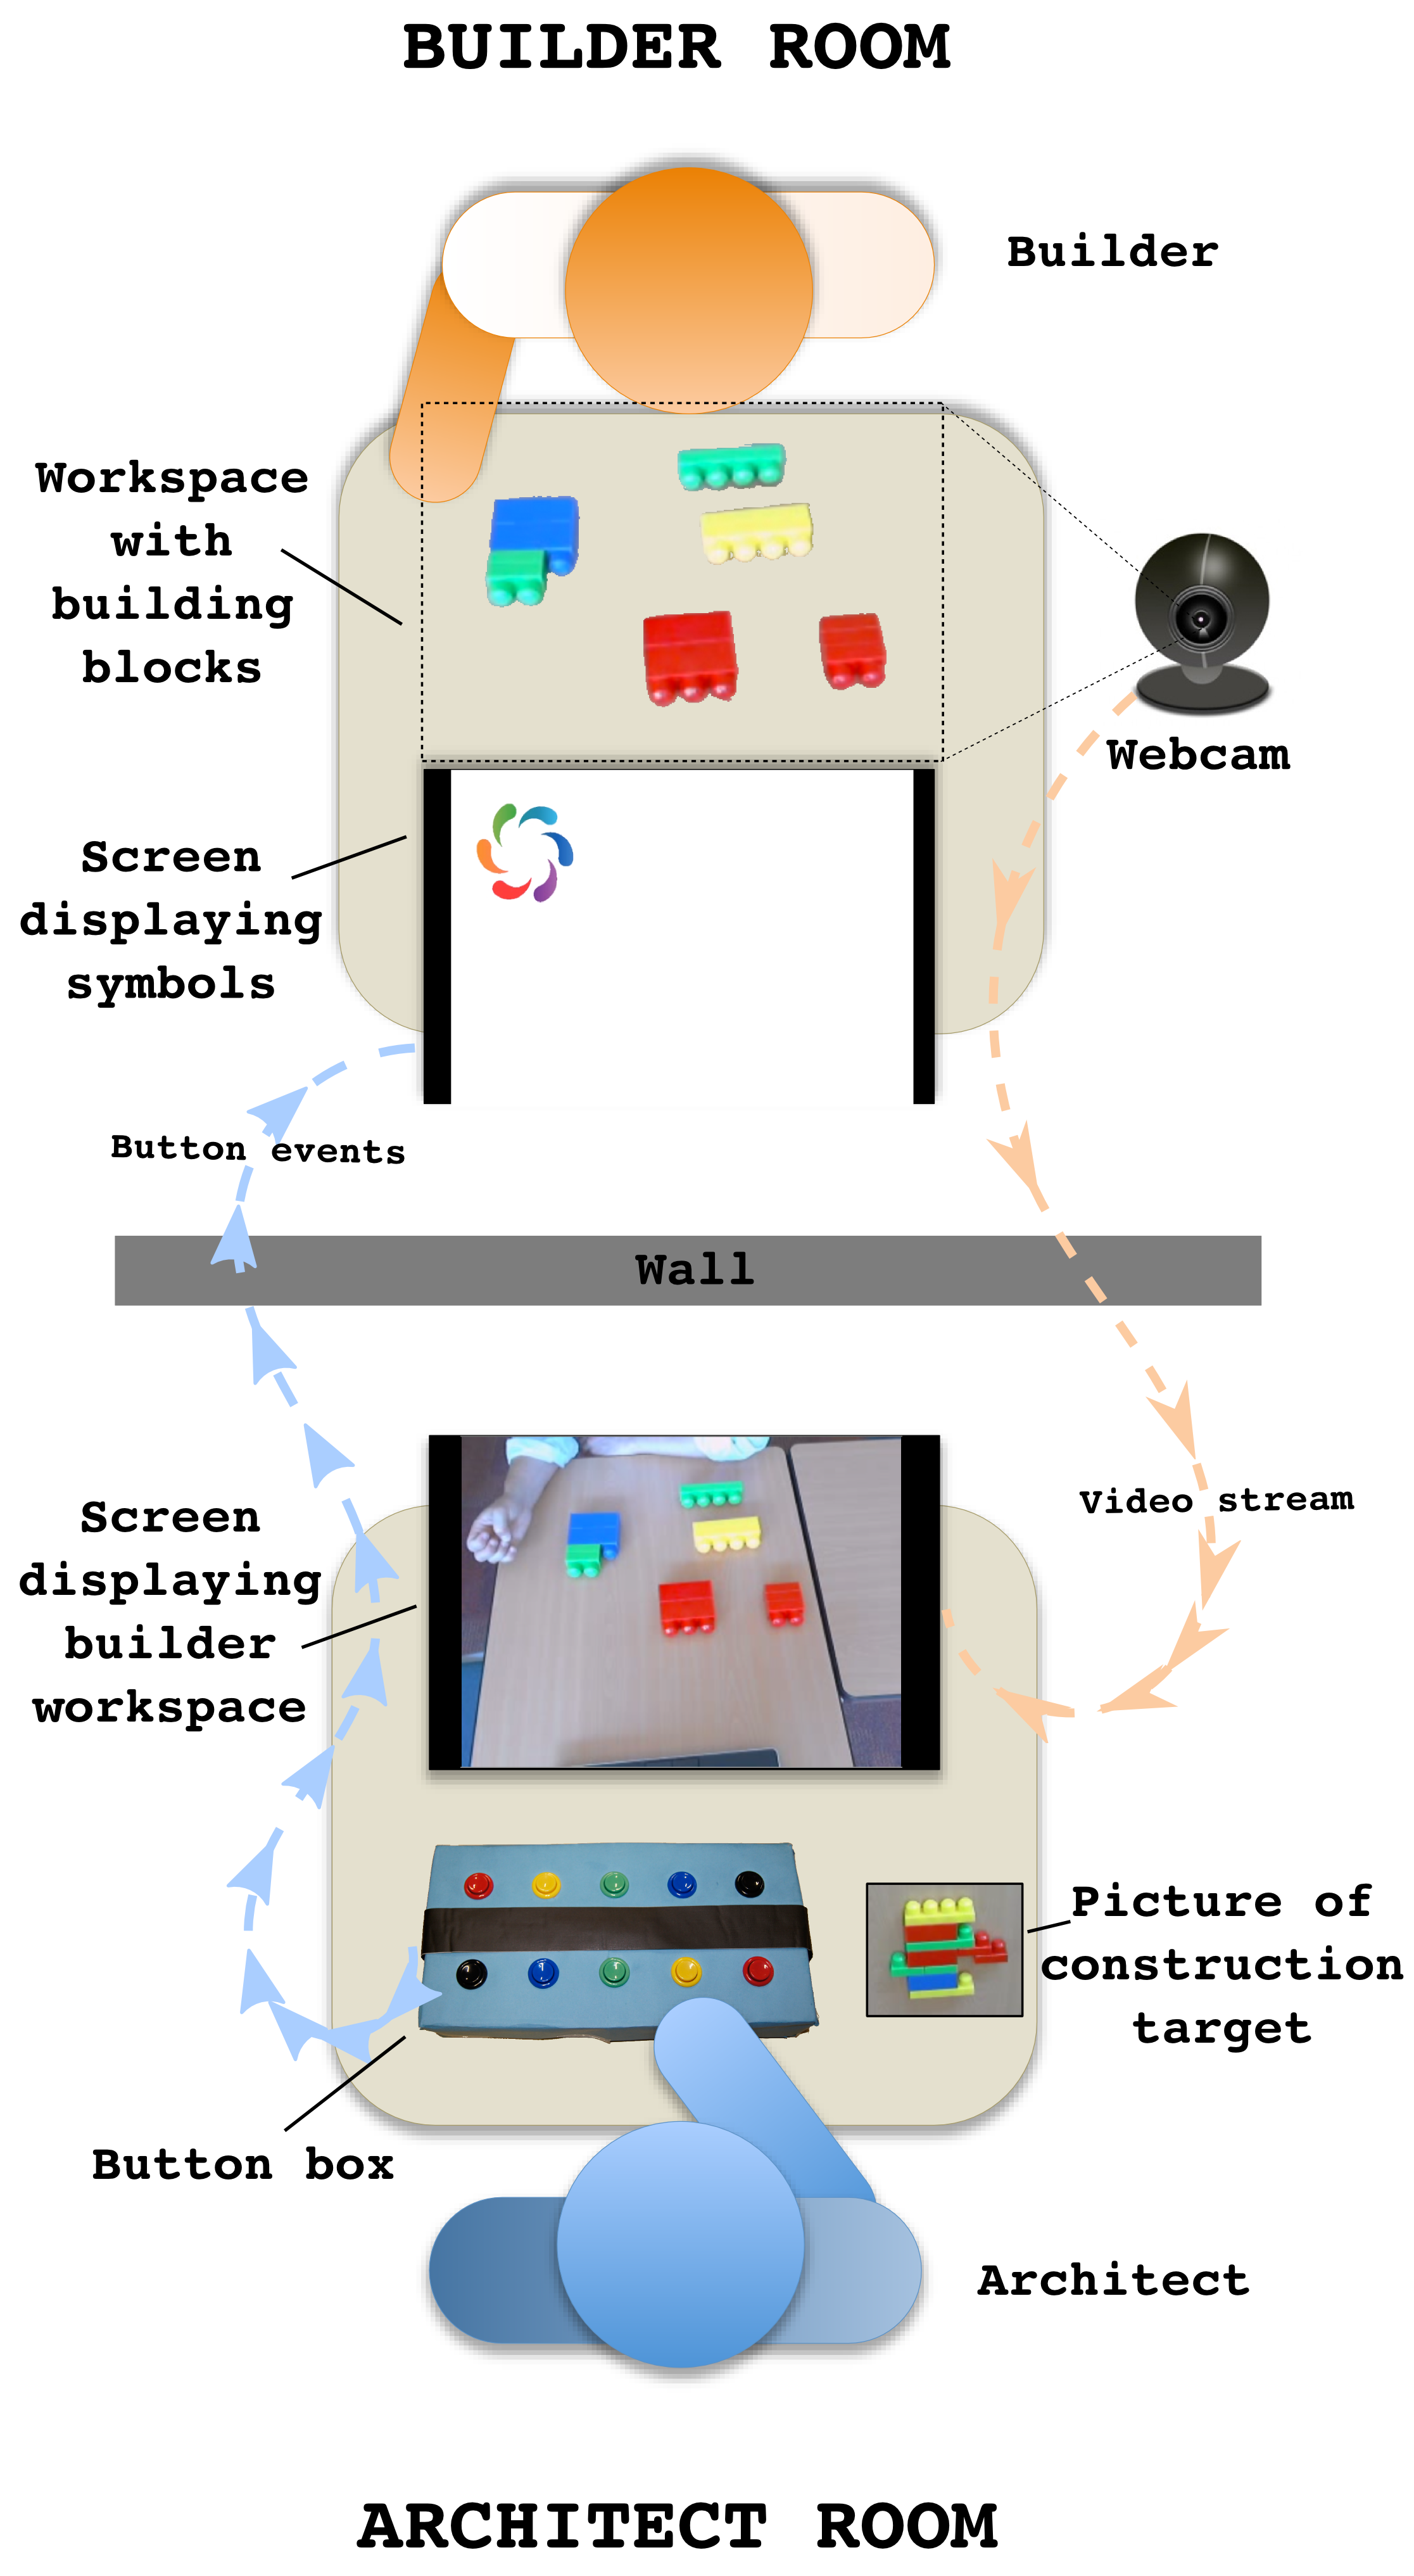
\includegraphics[width=0.68\columnwidth]{\visualspng/humanexp/setup/setup_normal_video_one_column.png}
\caption{Schematic view of our experimental setup. An architect (bottom) and a builder (top) should collaborate in order to build the construction target while located in different rooms. The architect has a picture of the targeted construction, while the builder has access to the construction blocks. The communication between them is restricted. The architect only sees a top view of the builder's workspace and can communicate with the builder only though the use of 10 buttons which, when pressed, display symbols on a screen on the builder side.}
\label{fig:overviewsetup}
\end{figure}

Figure~\ref{fig:overviewsetup} gives an overview of the experimental setup which considers an architect and a builder that are each seated at a table in front of a computer screen in two separate rooms and can neither hear nor see each other. 

The builder is equipped with a set of building blocks, in our case with 12 primary-colored Mega Bloks\textsuperscript{\textregistered} toy blocks differing in shape and color (see Figure~\ref{fig:bricks}). There were three red two-pads, two red three-pads, two yellow four-pads, two blue three-pads, two green two-pads, and one green four-pads blocks. 

The goal of the game is to assemble a specific construction yet unknown to the builder. As exemplified in Figure~\ref{fig:structures}, a construction is a flat combination of several blocks at least linked to one another by one pad. It does not necessarily contain all available blocks.

\begin{figure}[!htbp]
\centering
\begin{subfigure}[b]{0.49\columnwidth}
          \centering
          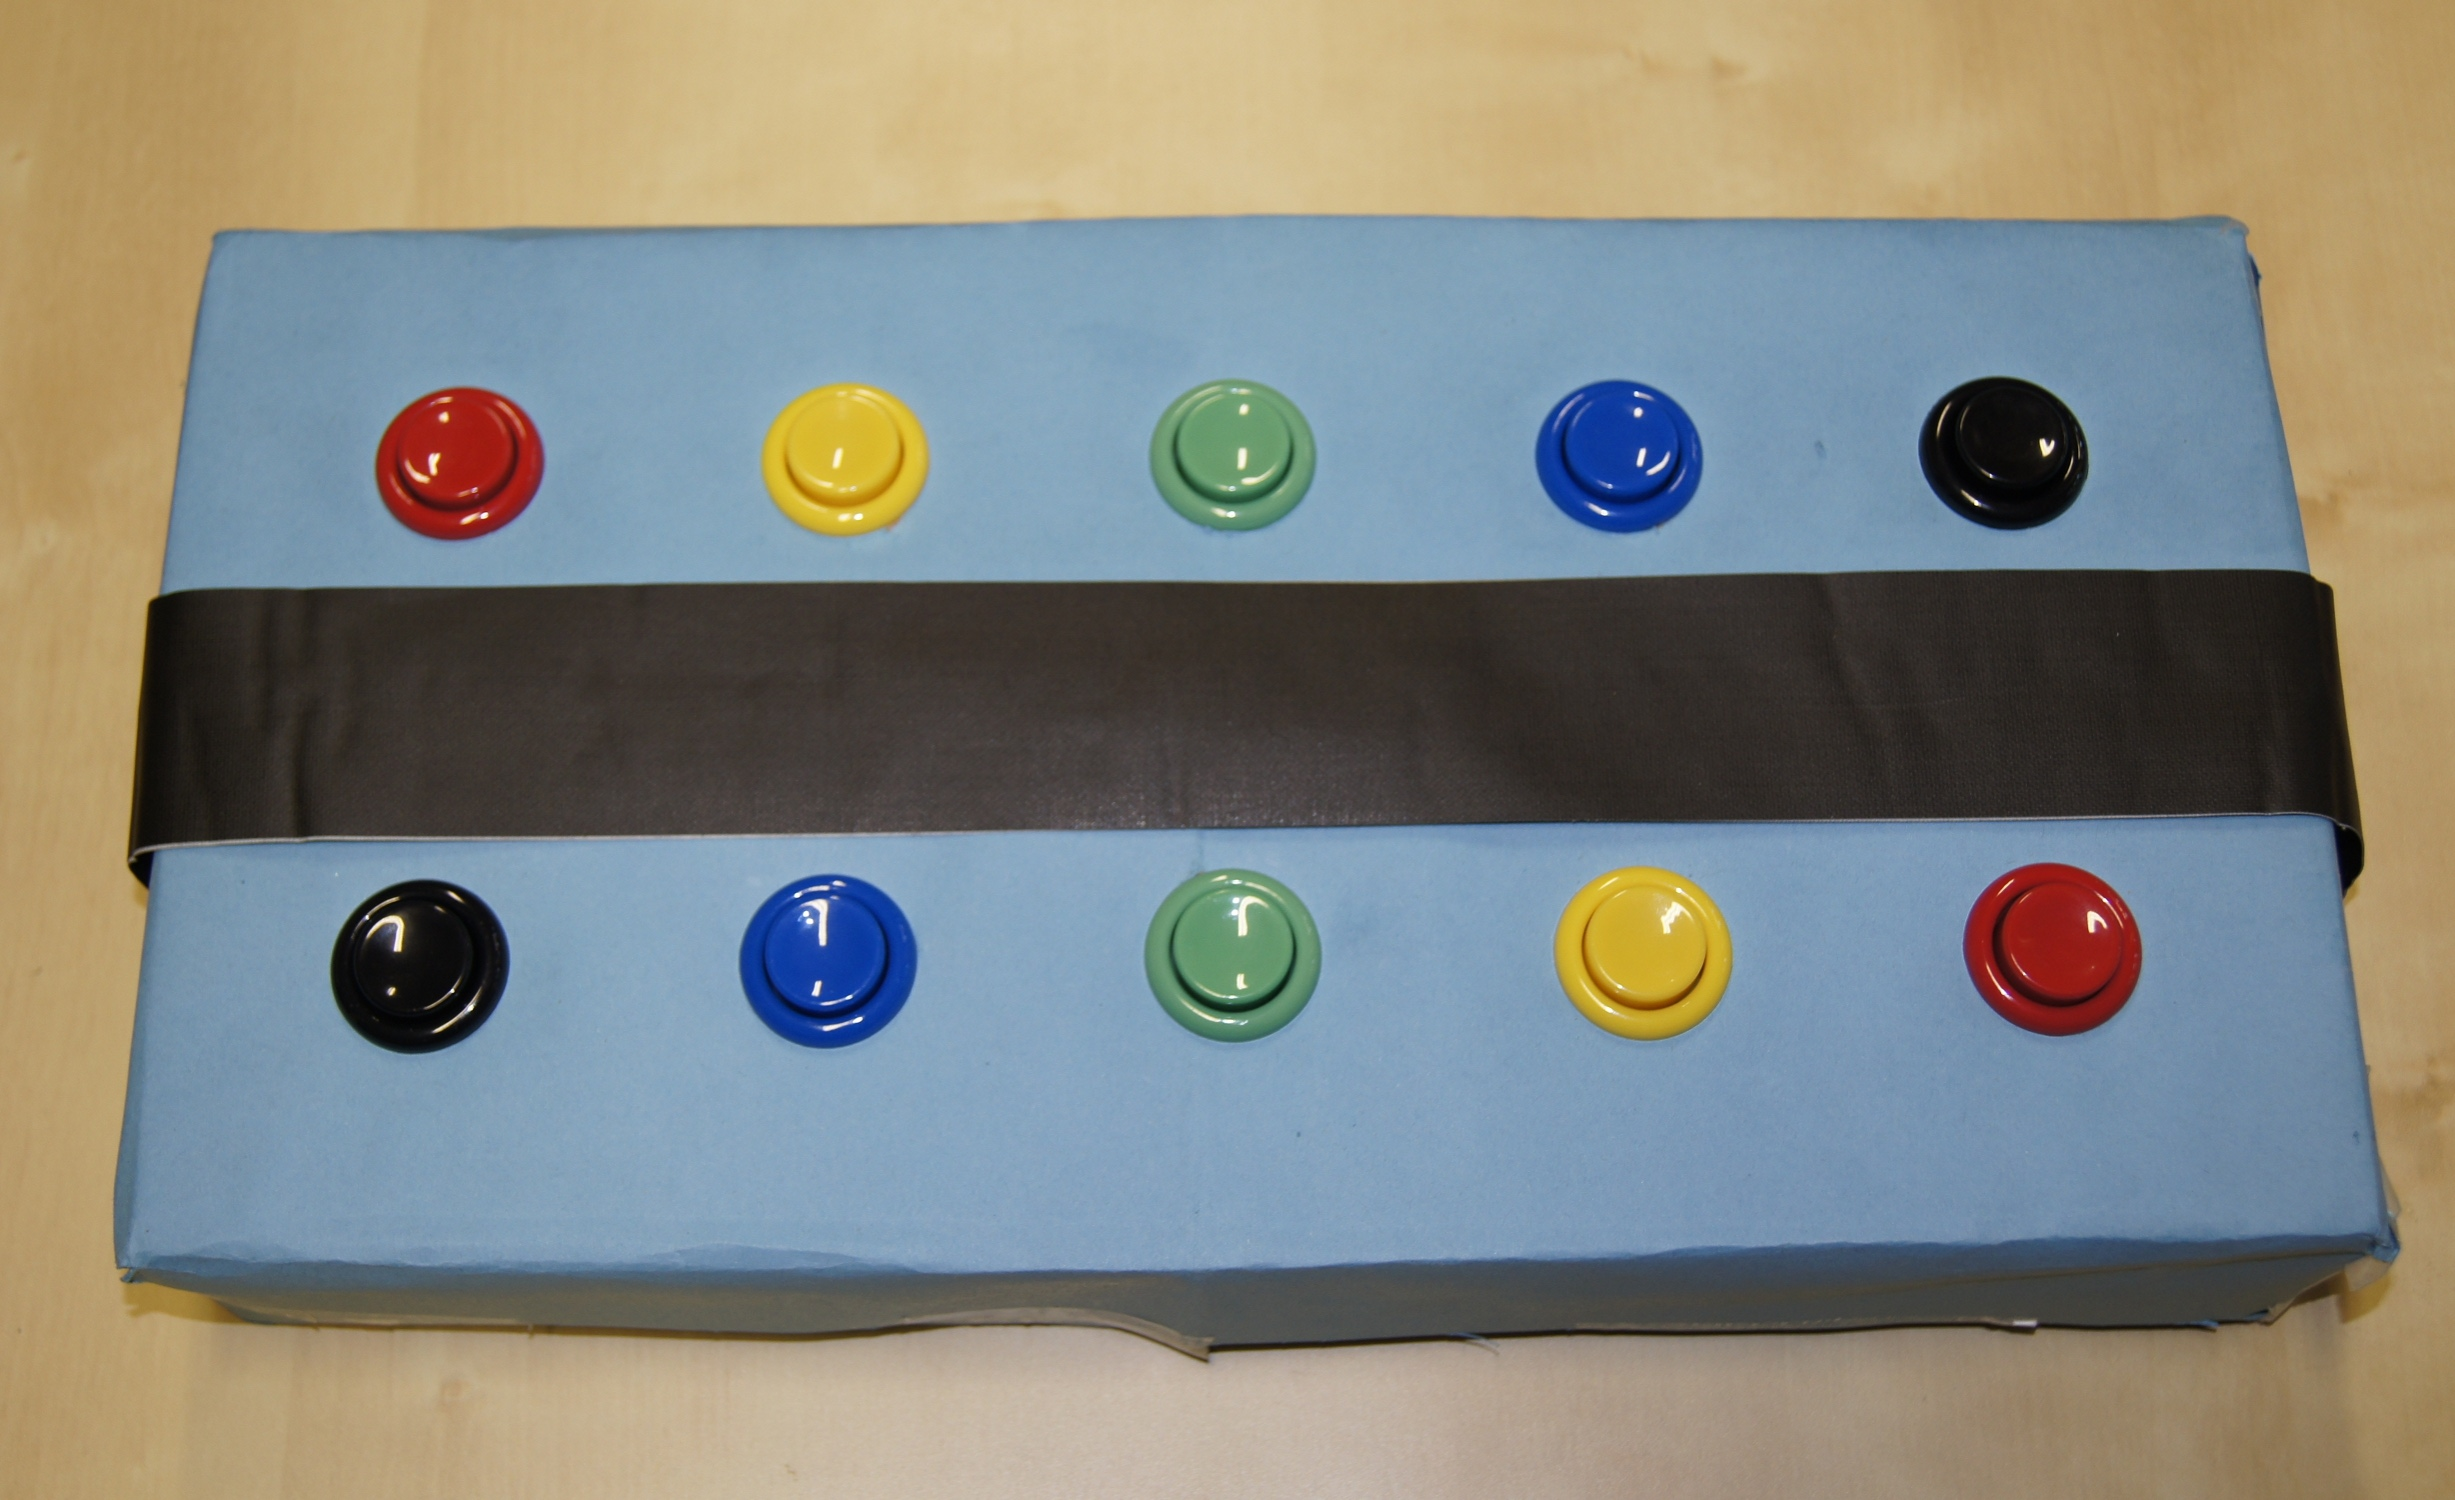
\includegraphics[height=3cm]{\imgpath/box.jpg}
          \caption{The box and the buttons used as an interface for the architect to communicate with the builder.}
          \label{fig:box}
\end{subfigure}
\begin{subfigure}[b]{0.49\columnwidth}
          \centering
          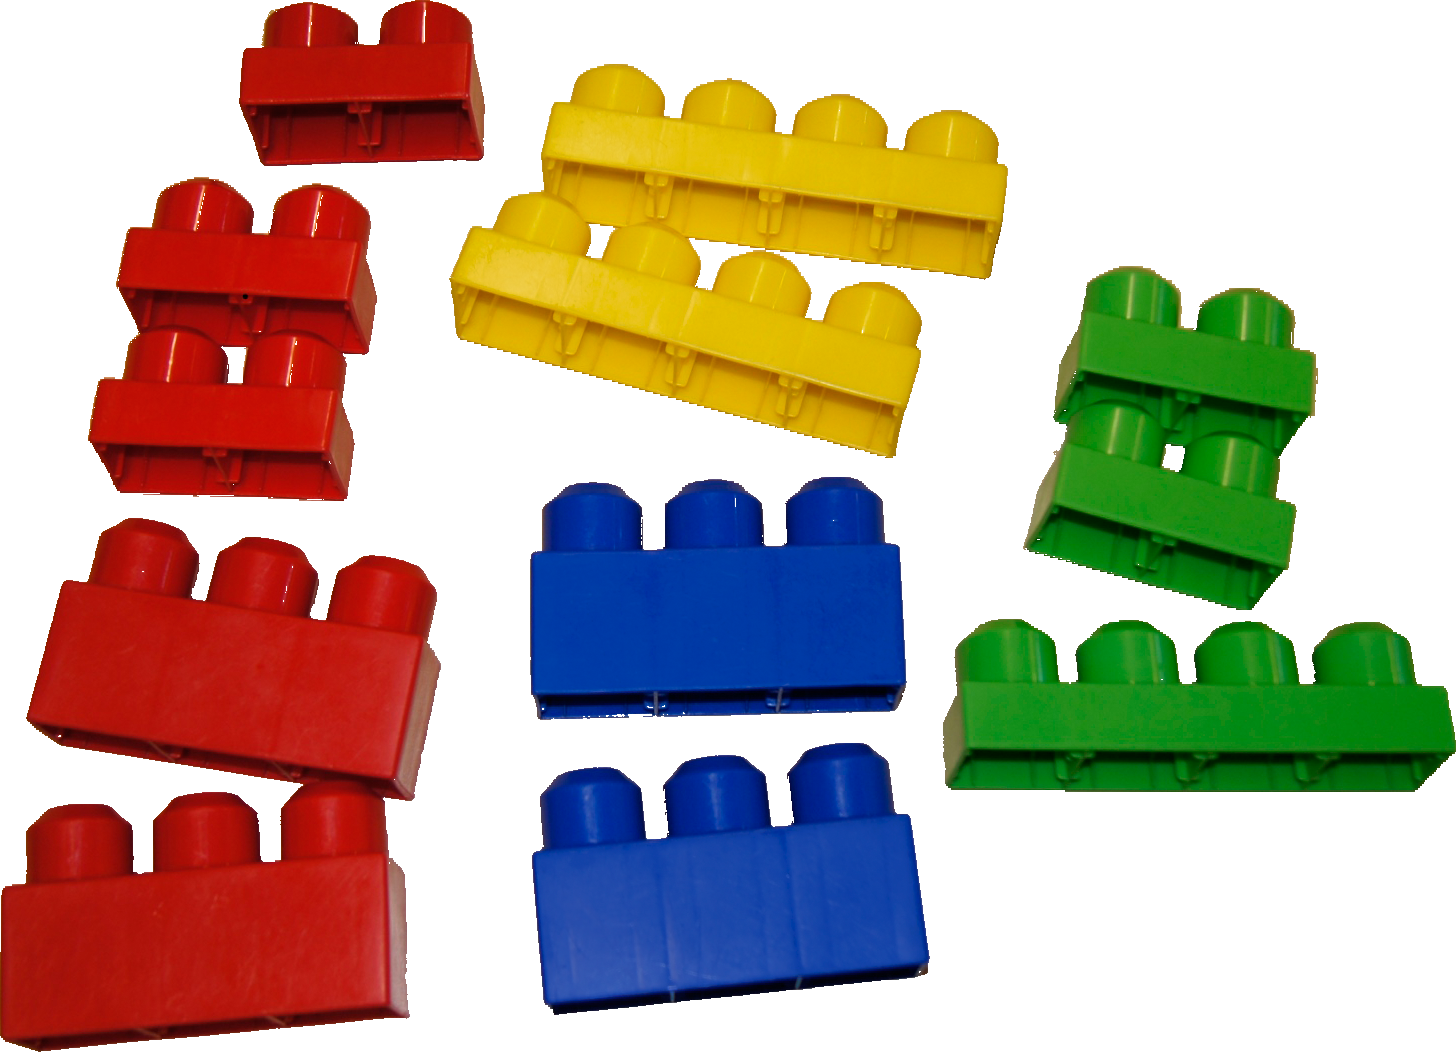
\includegraphics[height=3cm]{\imgpath/bricks.png}
          \caption{All toy blocks used in the collaborative construction task.}
          \label{fig:bricks}
\end{subfigure}
\caption{Elements of the setup.}
\label{fig:stuff}
\end{figure}

\begin{figure}[!htbp]
    \centering
    \begin{subfigure}[b]{0.24\columnwidth}
        \centering
        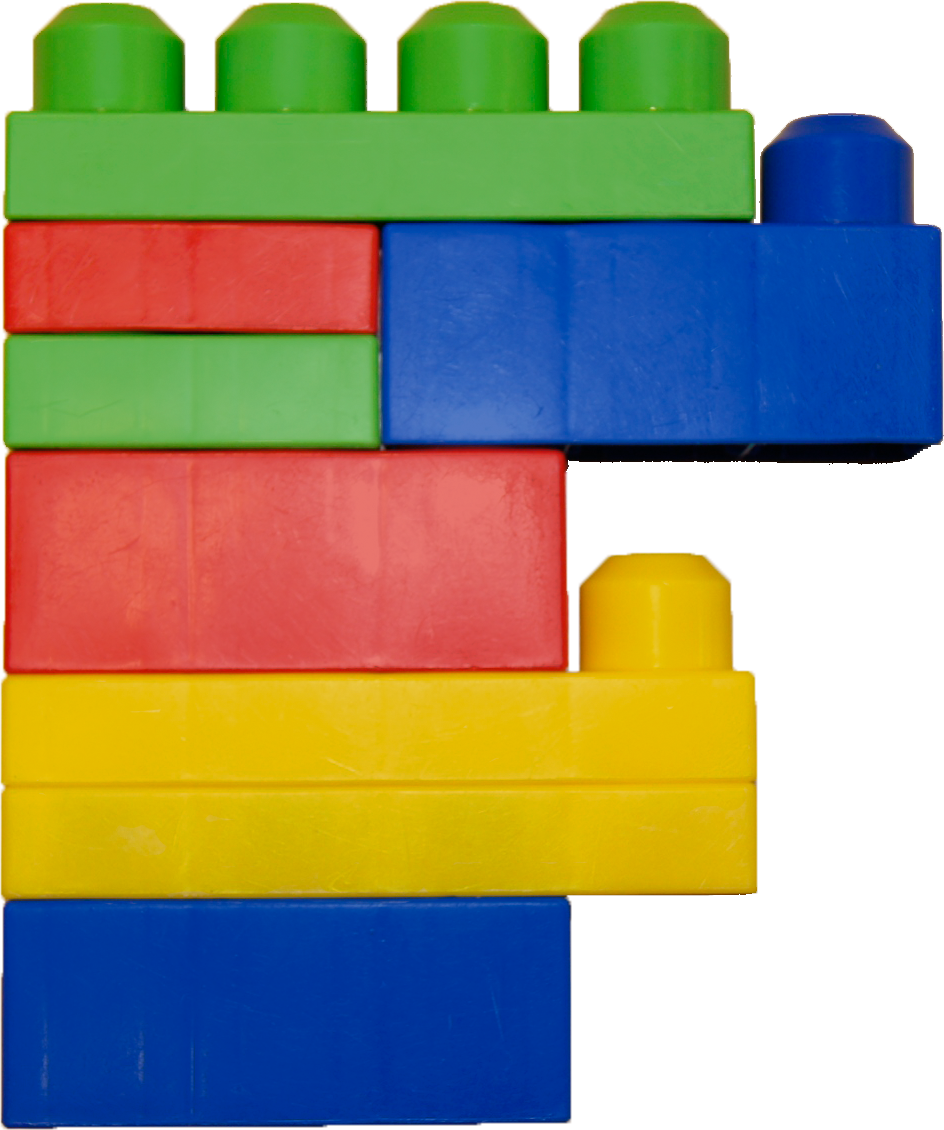
\includegraphics[height=3cm]{\imgpath/struct1.png}
        \caption{}
    \end{subfigure}
    \begin{subfigure}[b]{0.74\columnwidth}
        \centering
        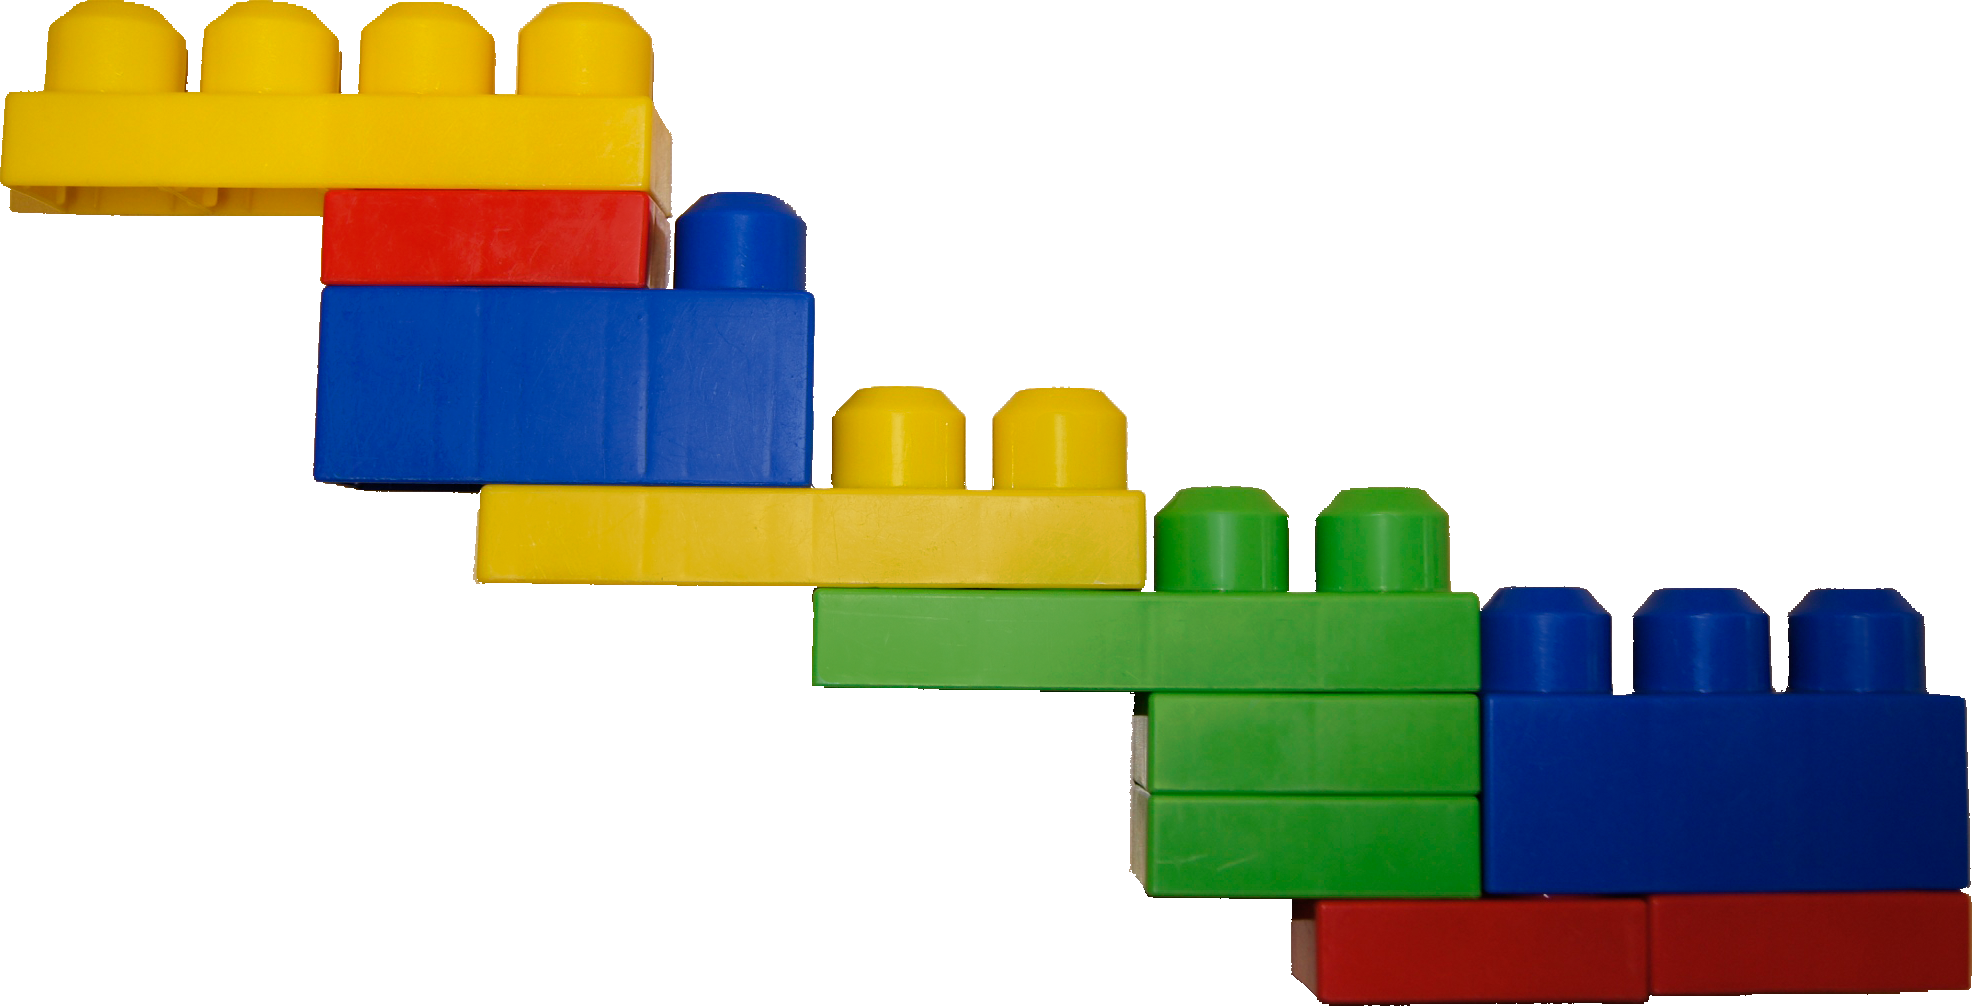
\includegraphics[height=3cm]{\imgpath/struct2.png}
        \caption{}
    \end{subfigure}
    \begin{subfigure}[b]{0.49\columnwidth}
        \centering
        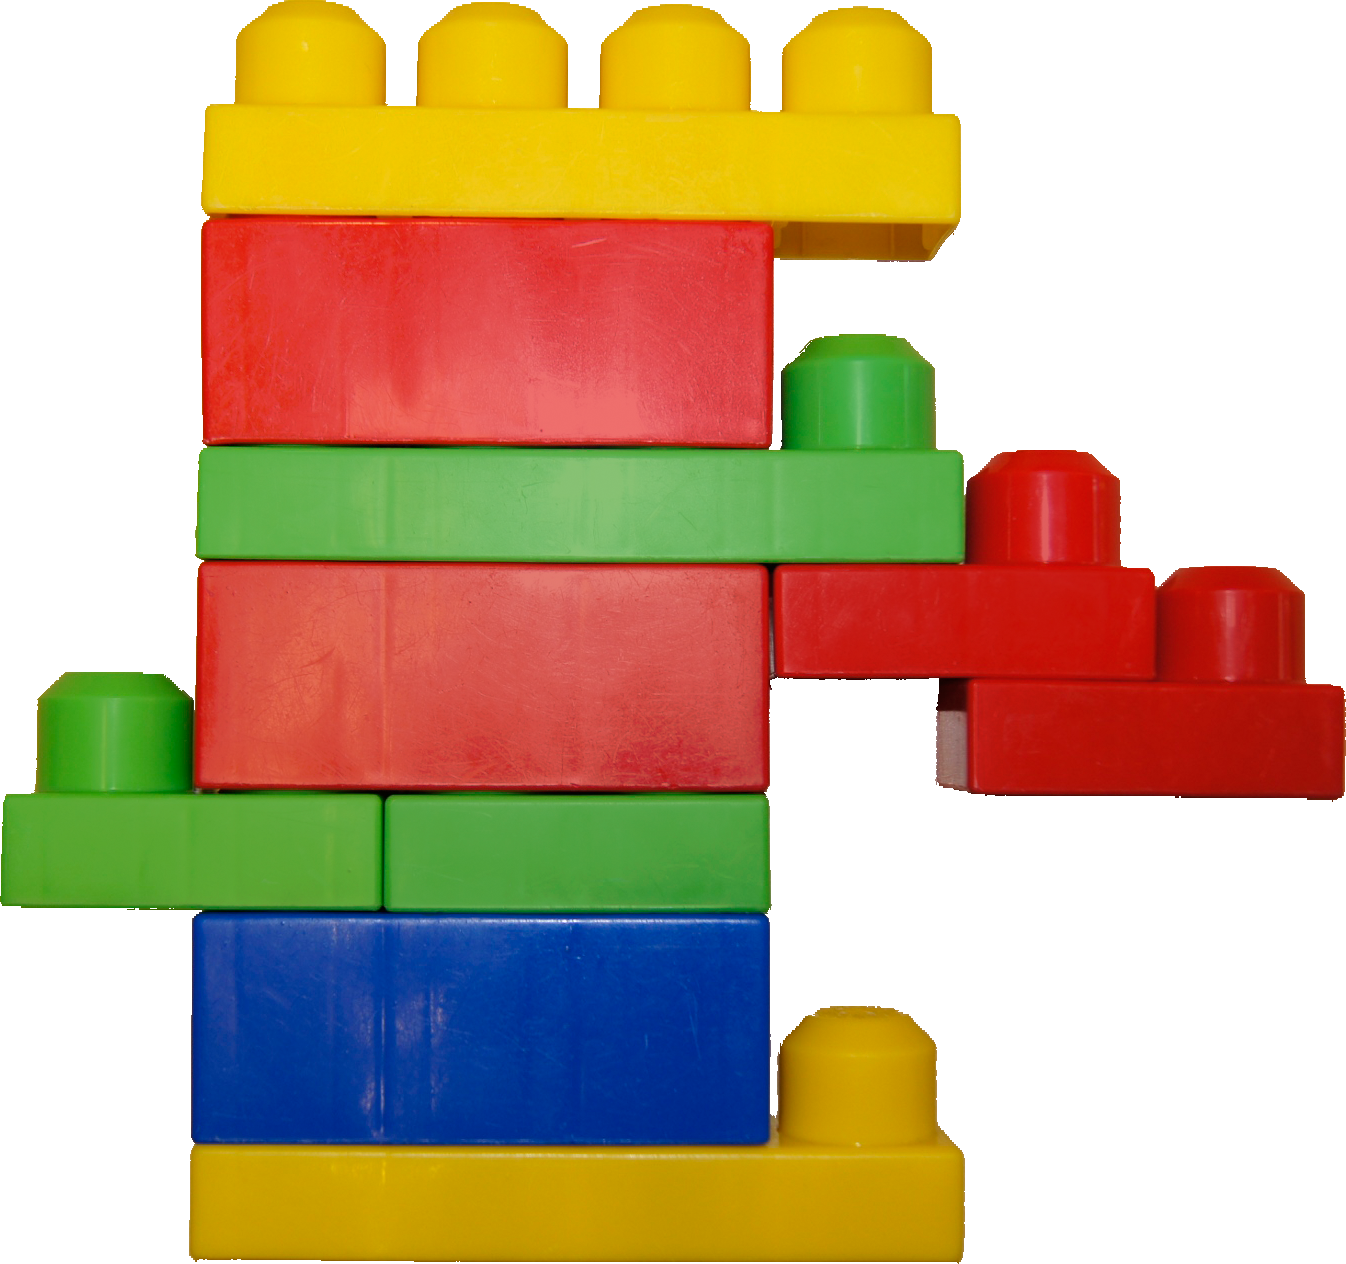
\includegraphics[height=3cm]{\imgpath/struct3.png}
        \caption{}
        \label{fig:sc}
    \end{subfigure}
    \begin{subfigure}[b]{0.49\columnwidth}
        \centering
        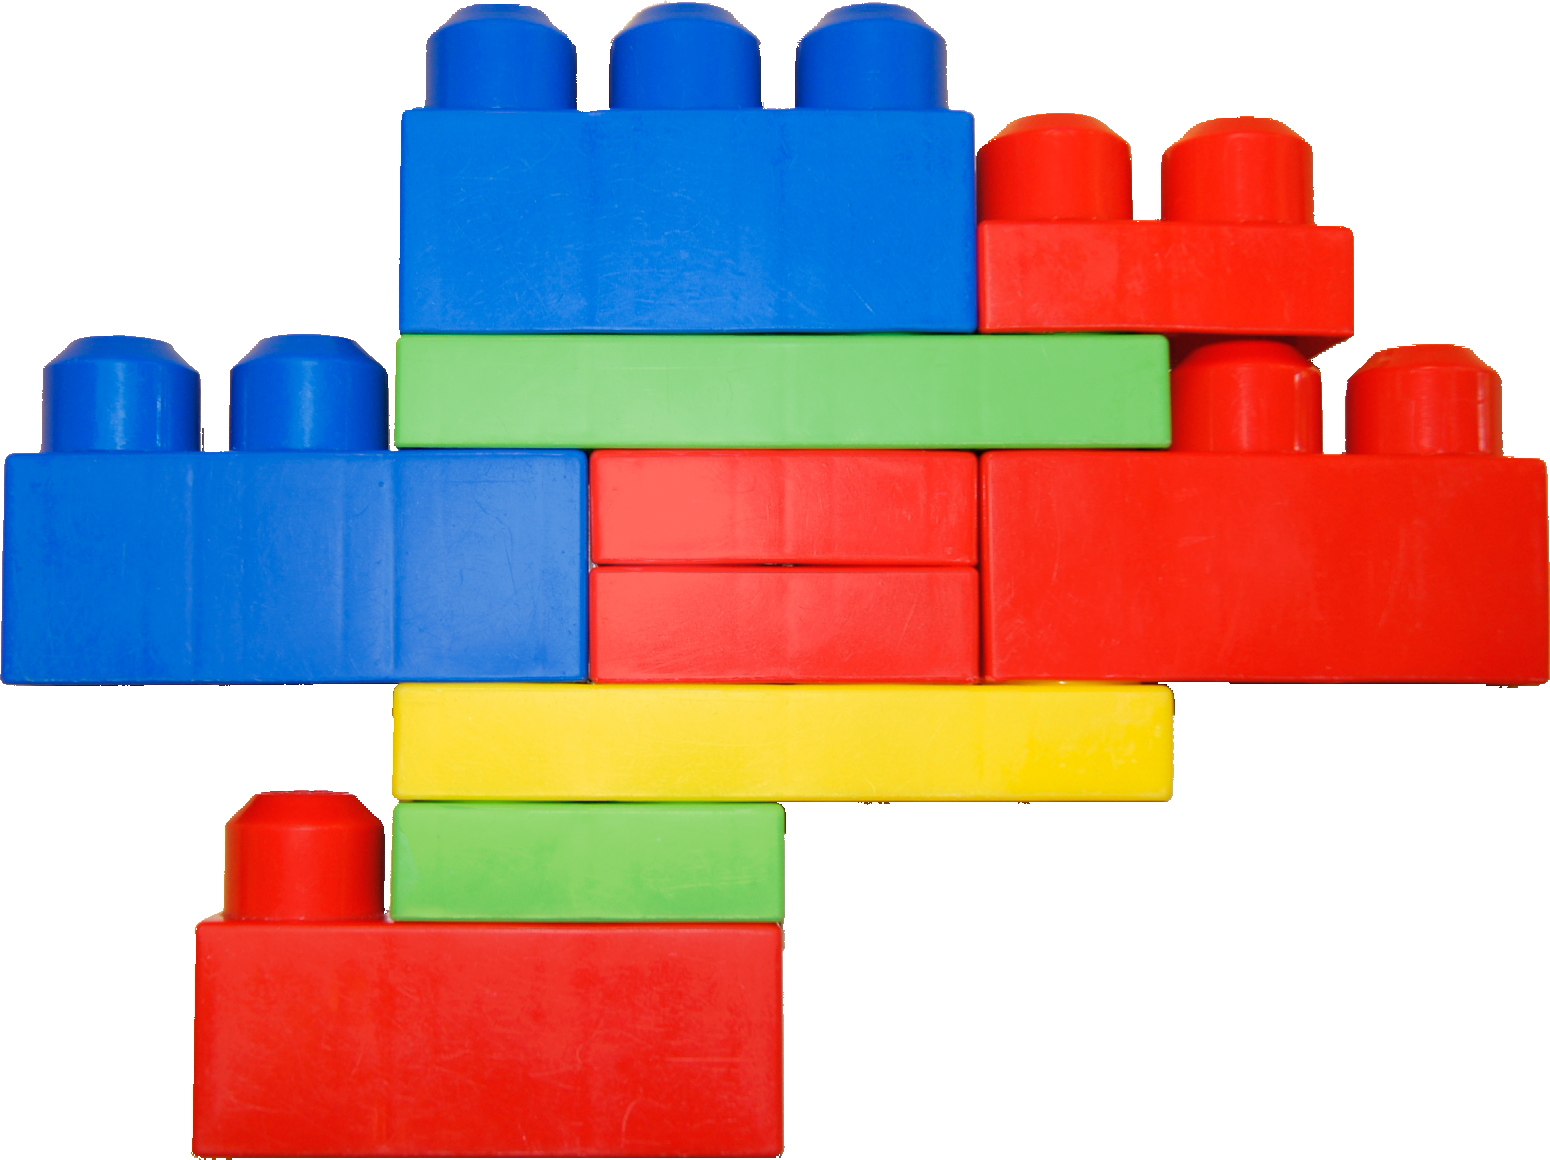
\includegraphics[height=3cm]{\imgpath/struct4.png}
        \caption{}
    \end{subfigure}
    \caption{Four examples of target structures presented to the architect.} 
    \label{fig:structures}
\end{figure}

The architect is given an image of the specific construction to be build and is told to guide the other player building it. A screen displays a live top view of the builder workspace. To communicate with the builder, the architect has access to a rudimentary interface made of 10 buttons, see Figure~\ref{fig:box}. Pressing a button displays a symbol on the screen located in the builder room. Each button is mapped to one of ten symbols and one of ten positions (two rows of five symbols) on the builder's screen, whereby the spacial organization of buttons differs from the spatial organization of displayed symbols. The mapping is randomized for each subject and fixed for the duration of one game. Figure~\ref{fig:sign} shows the different symbols.

\begin{figure}[!htbp]
\centering

\includegraphics[width=\columnwidth]{\visualspdf/humanexp/signs/signs.pdf}
\caption{The ten signs displayed on the builder screen.}
\label{fig:sign}
\end{figure}

\subsection{Participants}

We recruited 22 participants (19 m, 3 f) among students and staff at INRIA Bordeaux Sud-Ouest. Their age range was between 20 and 35 ($M = 25, SD = 3.91$) years. They played the collaborative game in pairs, where the two players in a pair were assigned randomly to the roles of a builder and an architect. Seven of the eleven pairs played the game together twice, such that each of the 14 participants involved assumed each role once. One second round of a dyad was excluded from the analyses, because the architect neglected the task instructions and altered the target structure during the game. This resulted in a total of 17 rounds.

\subsection{Procedure}
\label{sec:procedure}
Participants were not given the chance to talk about the game before it began. Architect and builder were instructed about their respective roles separately in their respective rooms. We presented the architects with a set of 20 pictures of different constructions from which they chose one. The builder was informed about the constraint that applied on the construction, i.e. flat construction which does not necessarily contain all available blocks. The architect and the builder were specifically told that the button positions did not directly map onto the symbols' positions displayed on the builder's screen, but that the mapping was fixed and arbitrary. Additionally, because the architect could see the hands of the builder during the game (see Figure~\ref{fig:overviewsetup}), the builder is told to only use his/her hands to move blocks and not to use hand signs. In practice, this was well respected by participants.

The game was \textbf{not} preceded by any training sessions. We aimed at reducing the time between the instruction of the participants and the beginning of the game as much as possible, so that they did not have time to elaborate any concrete strategy before the game began.

Once the game started, we observed the behavior of the two players and asked them to speak aloud about the meaning associated to the symbols/buttons. The experimenters took notes on the participants' remarks. The experiment stopped only when the builder decided and told the experimenters that the structure he had build was correct.

% During the experiments, the architects and builders were ask to speak aloud respectively what meaning they intended to convey by pressing a button and what they understood from the symbols displayed on the screen.

%%%%%%%%%%%%%%%%%%%%%%%%%%%%%%%%%%%%%%%%%%%%%%
%%%%%%%%%%%%%%%%%%%%%%%%%%%%%%%%%%%%%%%%%%%%%%
%%%%%%%%%%%%%%%%%%%%%%%%%%%%%%%%%%%%%%%%%%%%%%
%%%%%%%%%%%%%%%%%%%%%%%%%%%%%%%%%%%%%%%%%%%%%%
%%%%%%%%%%%%%%%%%%%%%%%%%%%%%%%%%%%%%%%%%%%%%%
\section{Results}

As stated before, the current pilot study serves as a proof of concept. We aimed at designing a setup allowing to study the processes involved in the formation of interaction protocols in asymmetric interaction with the particular constraint that the players could neither solve the task by themselves nor did they have access to any reward function.

Our pilot study revealed a great potential in the use of our experimental method to study many aspects of communication relevant to HRI. With our setup, we will be able to study, among others, questions related to alignment, rhythm, contingency, and feedback, which have been in the focus of HRI research for some time \cite{kopp2010social,michalowski2007dancing,fischer2013impact,vollmer2014robots,pitsch2013robot,wrede2010appropriate}.

Surprisingly, while the construction task in this setup seems really challenging on paper and participants thought they would never succeed, a majority of the architect-builder pairs succeeded on building the correct construction. We analyzed a total of 17 experiments, of which 13 were successful and 4 failed. The average duration of the runs was 18 minutes ($M = 18~min, SD = 11~min$) with a minimum of 7 minutes and a maximum of 45 minutes.

In what follows, we showcase results supporting our claim that our setup can be used to study the co-construction of meaning in restricted, asymmetric interaction. We will first show one run of the game in detail which should give the reader an idea about what happens during an interaction and the richness and aptness of the data to consider a variety of research questions. Then, we will continue with presenting our results on the negotiation of signal meanings and with describing observations of the builder behavior. We will conclude with mentioning interesting additional considerations which are beyond the scope of this work.

\subsection{One experiment in detail} 
\label{sec:case}

Figure~\ref{fig:timeline} brings together information about button presses (logs), their intended and interpreted meanings (found by the experimenters from their notes and observations of logs), and the builder's actions (builder video of the construction workspace) and makes clear the bi-directionality of the interaction. On the bottom of the figure, we see that the builder proposes blocks to the architect (blocks not belonging to the target structure in black, blocks belonging to it in gray) (cf. Subsection~\ref{sec:builder}) and on the top we see how the architect responds to the builder's actions in terms of button presses and meanings. Additionally, we see how the builder interprets these signals of button presses which he/she perceives as symbols on a screen (middle timeline of button presses and meanings) and how these interpretations and believes in turn again influence what the builder does next.

\begin{figure}[!htbp]
\begin{widepage}
\centering
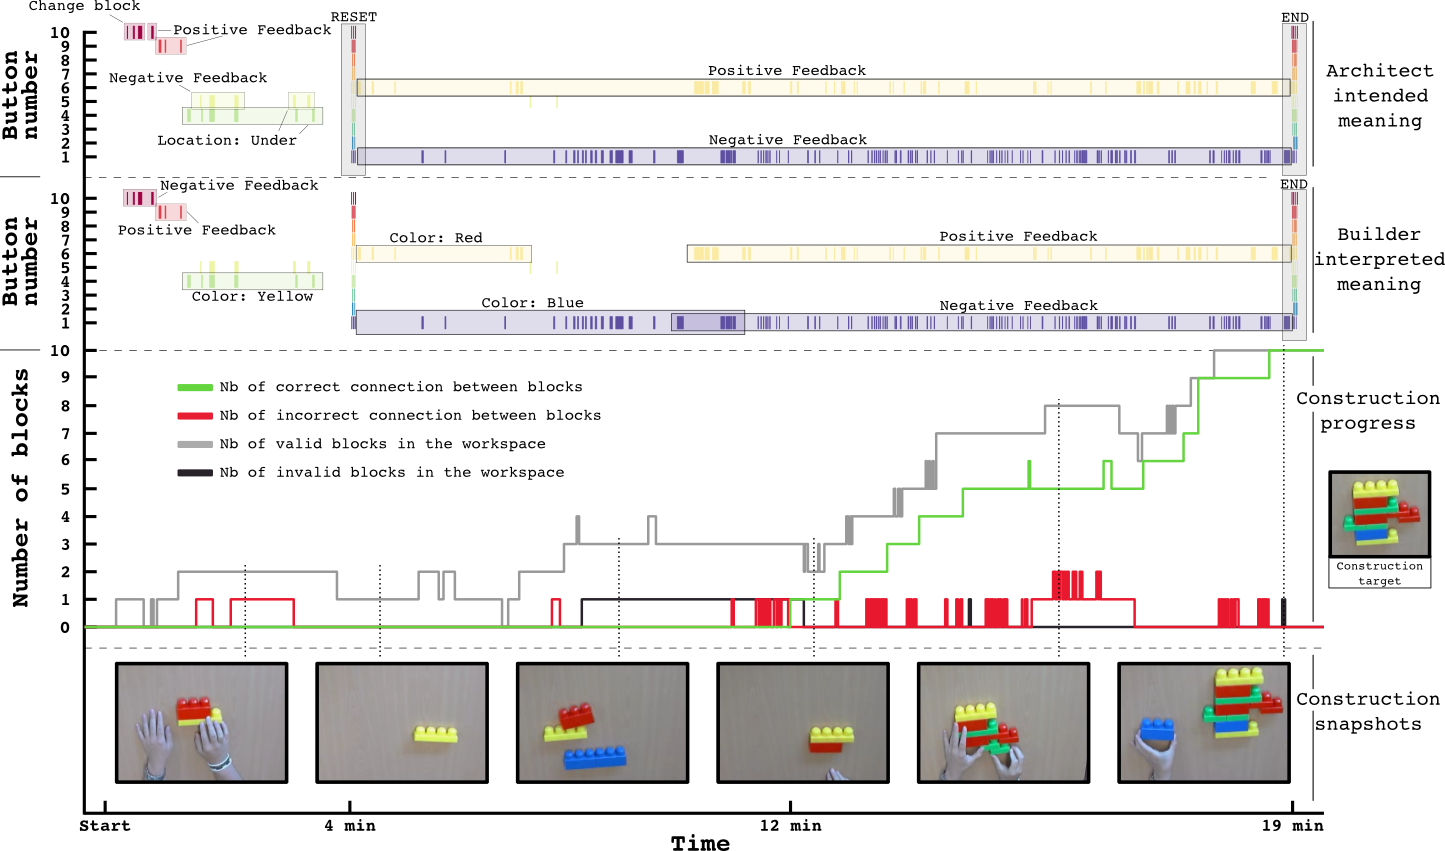
\includegraphics[width=1\textwidth]{\visualspng/humanexp/timeline/timeline_with_visu.png}
\end{widepage}
\caption{Timeline for one experiment of an architect and a builder collaborating towards building the construction target (right hand side). The top and middle part show the timeline of button presses associated with the intended meaning from the architect (top) and the understood meaning from the builder (middle). There were 10 buttons, for which we logged all button presses for each experiment and here display all occurrences as colored dashes. The button events are annotated with the meaning the architect intended or the builder understood as participants reported during the game. Events that are not annotated were not mentioned by the participants. At the bottom, the figure additionally visualizes the progress made by the builder in assembling the target structure and also shows incorrect block propositions, joining of incorrect blocks and mistakes. These events were annotated by hand using the video annotation tool ELAN developed by the Max Planck Institute for Psycholinguistics, The Language Archive, Nijmegen, The Netherlands \cite{wittenburg2006elan}. A block proposition here started, when the transportation of the block towards the workspace ended and the block lay still on the table. It ended when the block was again picked up and subsequently removed from the workspace. These presentation events were classified into correct and incorrect propositions by determining whether the proposed block was part of the target structure. Equivalently, a joining event started when two blocks were successfully joined at either a correct or incorrect position (again depending on whether the resulting configuration was part of the target structure). It ended before right before the two previously joined blocks were again pulled apart.}
\label{fig:timeline}
\end{figure}

With respect to the meanings of the button presses, we observe changes of button meanings over the course of the interaction. The exact points in time when meaning changes occur have been matched to the button presses by hand and is therefore approximated. While this may be a problem for detailed analyses on a micro level, it is of little importance for the macro analysis presented here. During the first 4 minutes, the architect changes the intended meanings of signals many times and these meanings were not aligned with the builder's interpretation of signals. At 4 minutes, the architect presses all buttons at once, seemingly attempting to ask the builder to clear his/her mind and start over again. Right after this \emph{Reset} signal, the architect changes to one simple \emph{yes/no} strategy using button 1 and 6. On the builder's end, this Reset signal is followed by a pause of actions which hints at a direct confusion. It is only at 12 minutes into the game that the builder fully understands the intended meaning of the architect's button presses and can start joining two blocks correctly (green graph on the bottom). The experiment continues with the builder suggesting new blocks (bottom - black and gray events) and positions for new blocks (bottom - red and green events) one at a time which are validated or invalidated by the architect. After 19 minutes, the architect presses again all the buttons but this time with the aim of informing the builder that the construction is complete. The builder ended the experiment at that time. The \emph{End} signal was well interpreted by the builder as the interaction was going smoothly until that time and the few remaining blocks were rejected (bottom - black event at 19 min). The final construction was indeed the target one intended by the architect, hence resulting in a successful experiment.

Our setup allows to study the evolution of meanings associated to each button and put it in relation with the current context in the interaction. We find that the constraints inherent to our setup allow to analyze communication, especially the interplay of individual actions and their interactional history, as well as their concrete timing, while lowering interactional complexity and thereby reducing communicative noise.

\subsection{Meanings}

Architects and builders start the game without having agreed on specific meanings the buttons should convey. We start by studying the associated meanings obtained from our notes on signal meanings reported by builder and architect. They seemed to initially consider a large set of possible meanings, but, in the end, were able to agree primarily on only a limited number.

\paragraph{Types of Meanings} 

When analyzing the notes on the participants' explanation of signal meanings (see Subsection \ref{sec:procedure}), we identified nine different categories of meanings:

\begin{enumerate}
    \item \textbf{Positive Feedback}
    \item \textbf{Negative Feedback}
    \item \textbf{End}: The construction is finished.
    \item \textbf{Reset}: Start over.
    \item \textbf{Guidance}: Instruction on what to do. It includes \emph{change, invert, revert, new block, continue, stack}. 
    \item \textbf{Color}: Reference to the color of a block. It includes \emph{yellow, blue, red, green}.
    \item \textbf{Size}: Reference to the size of a block. It includes \emph{small, medium, big}.
    \item \textbf{Location}: Reference to the location of a block. It includes \emph{under, above, left, right}.
    \item \textbf{Group}: Reference to a group of blocks. It includes \emph{in, out, group\_X}.
\end{enumerate}

Importantly, those categories where \textbf{not} suggested to the participants beforehand, but only identified by us in a posteriori analysis.

For each experiment, we determined if the architect or the builder considered each type of meaning (see Figure~\ref{fig:types_of_feedback}). In every single experiment, positive and negative feedback were considered on both architect and builder side. The \emph{End} meaning has been considered on both sides in 14 experiments. More concrete instructions such as \emph{Guidance, Color, Size, or Location} were less often considered, especially by the builder.

\begin{figure}[!htbp]
  \begin{center}
      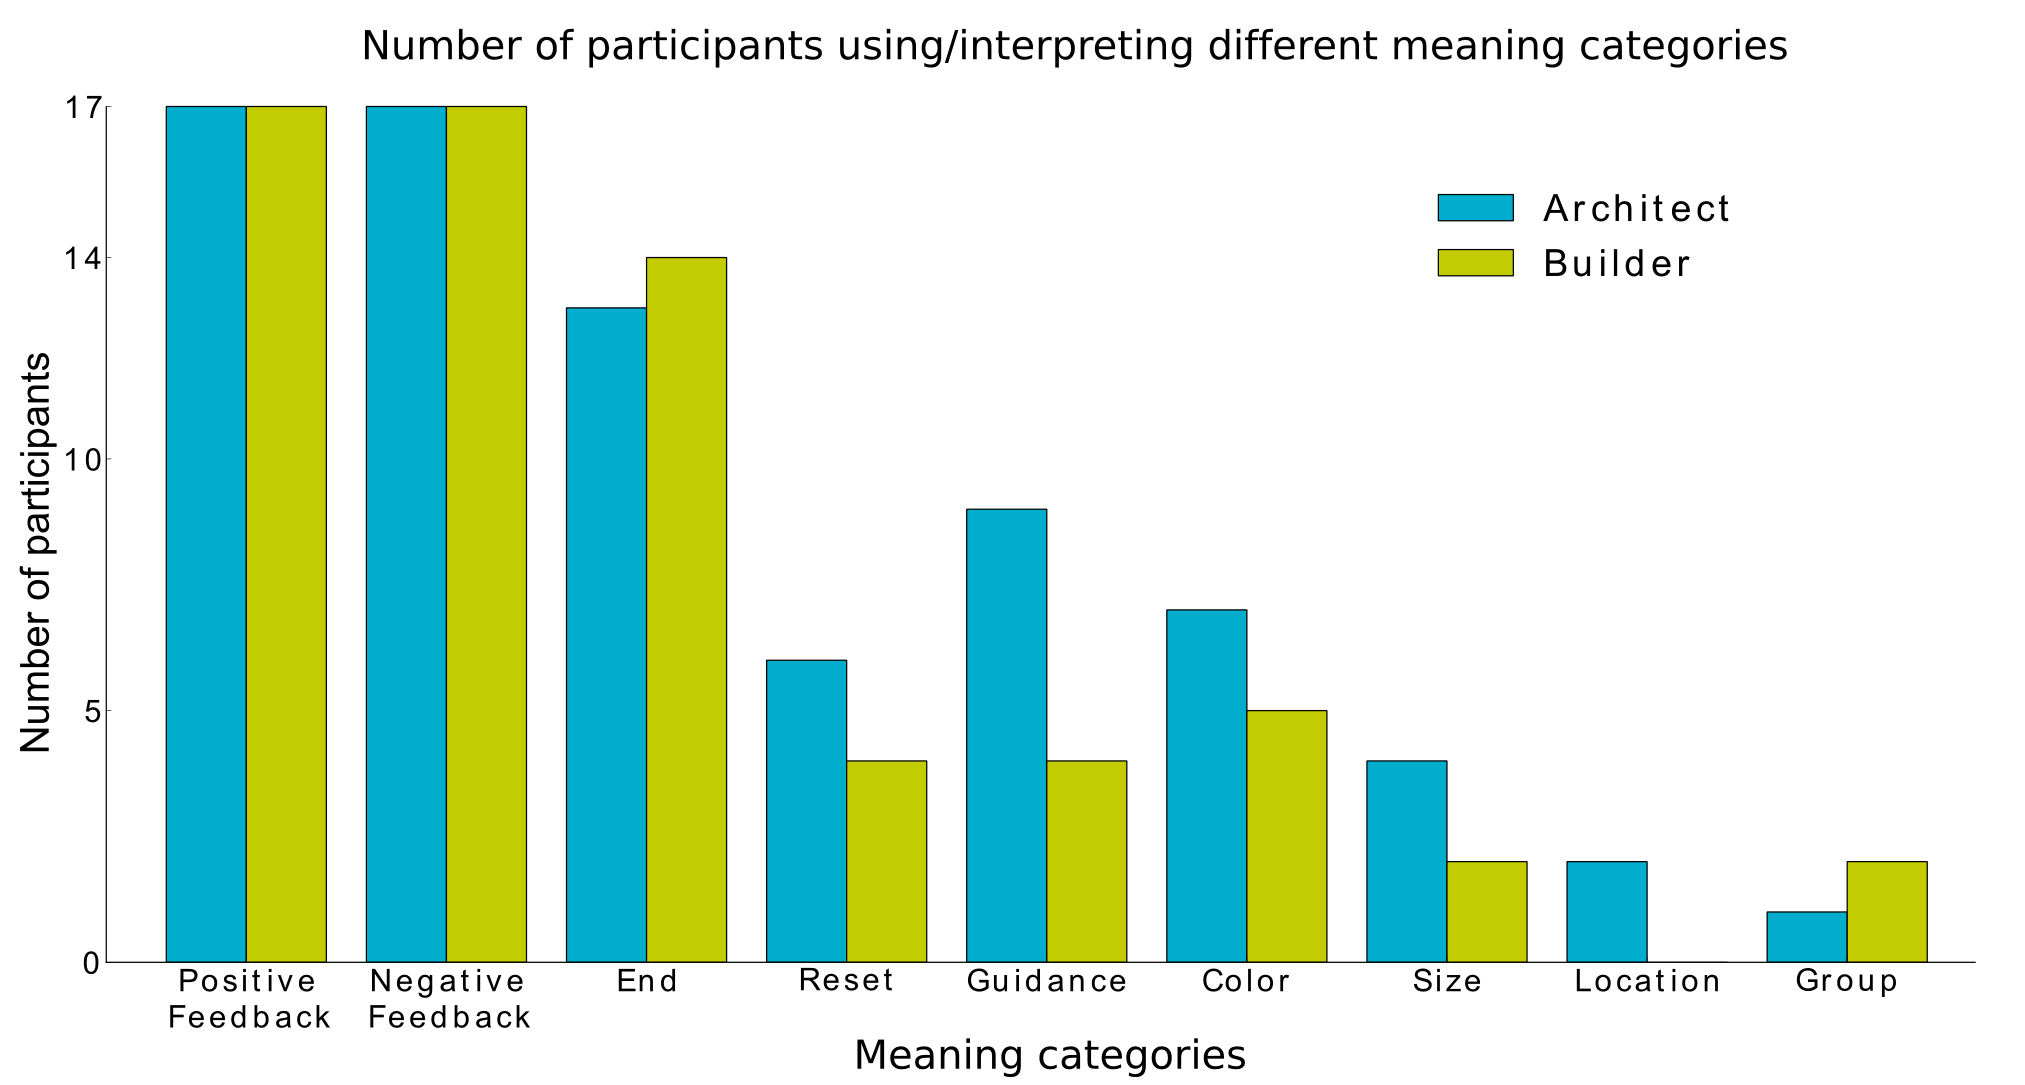
\includegraphics[width=\columnwidth]{\visualspdf/humanexp/meanings/instruction_type.pdf}
      \caption{Number of participants that used (architect) or interpreted (builder) signals as conveying different types of meaning. All participants considered positive and negative feedback.}
    \label{fig:types_of_feedback}
  \end{center}
\end{figure}

This is in line with the findings in \cite{griffiths2012bottom}, where ``correct'' and ``incorrect'' were also identified to be among the most common types of signal meanings.

\paragraph{Matching of meanings between architect and builder} 

Knowing which meaning categories were considered by each of the participants does not tell us if a particular pair of players understood each other. We therefore compared the associated meanings reported by architect and builder for all signals. Similarly to \cite{griffiths2012bottom}, we then determined the number of signals that were understood, misinterpreted, or ignored. We define signals which were understood as signals where both architect and builder agree on a common meaning. For signals which were misinterpreted, the builder reported a different associated meaning than the one intended by the architect. The signals which were mentioned by the architect, but not by the builder, were counted as ignored signals. We then averaged the results for successful and failed experiments, see figure~\ref{fig:types_of_understanding}. For successful experiments, the average number of signals understood is $M = 3.6, SD = 0.7$ which mostly corresponds to \emph{Positive feedback, Negative feedback, End}, and occasionally \emph{Reset} when needed (see Figure~\ref{fig:understanding_per_feedback}). Interestingly for failed experiments, this number drops to $M = 1.3, SD = 1.1$, with a larger amount of signals misinterpreted and ignored.

\begin{figure}[!htbp]
    \begin{center}
      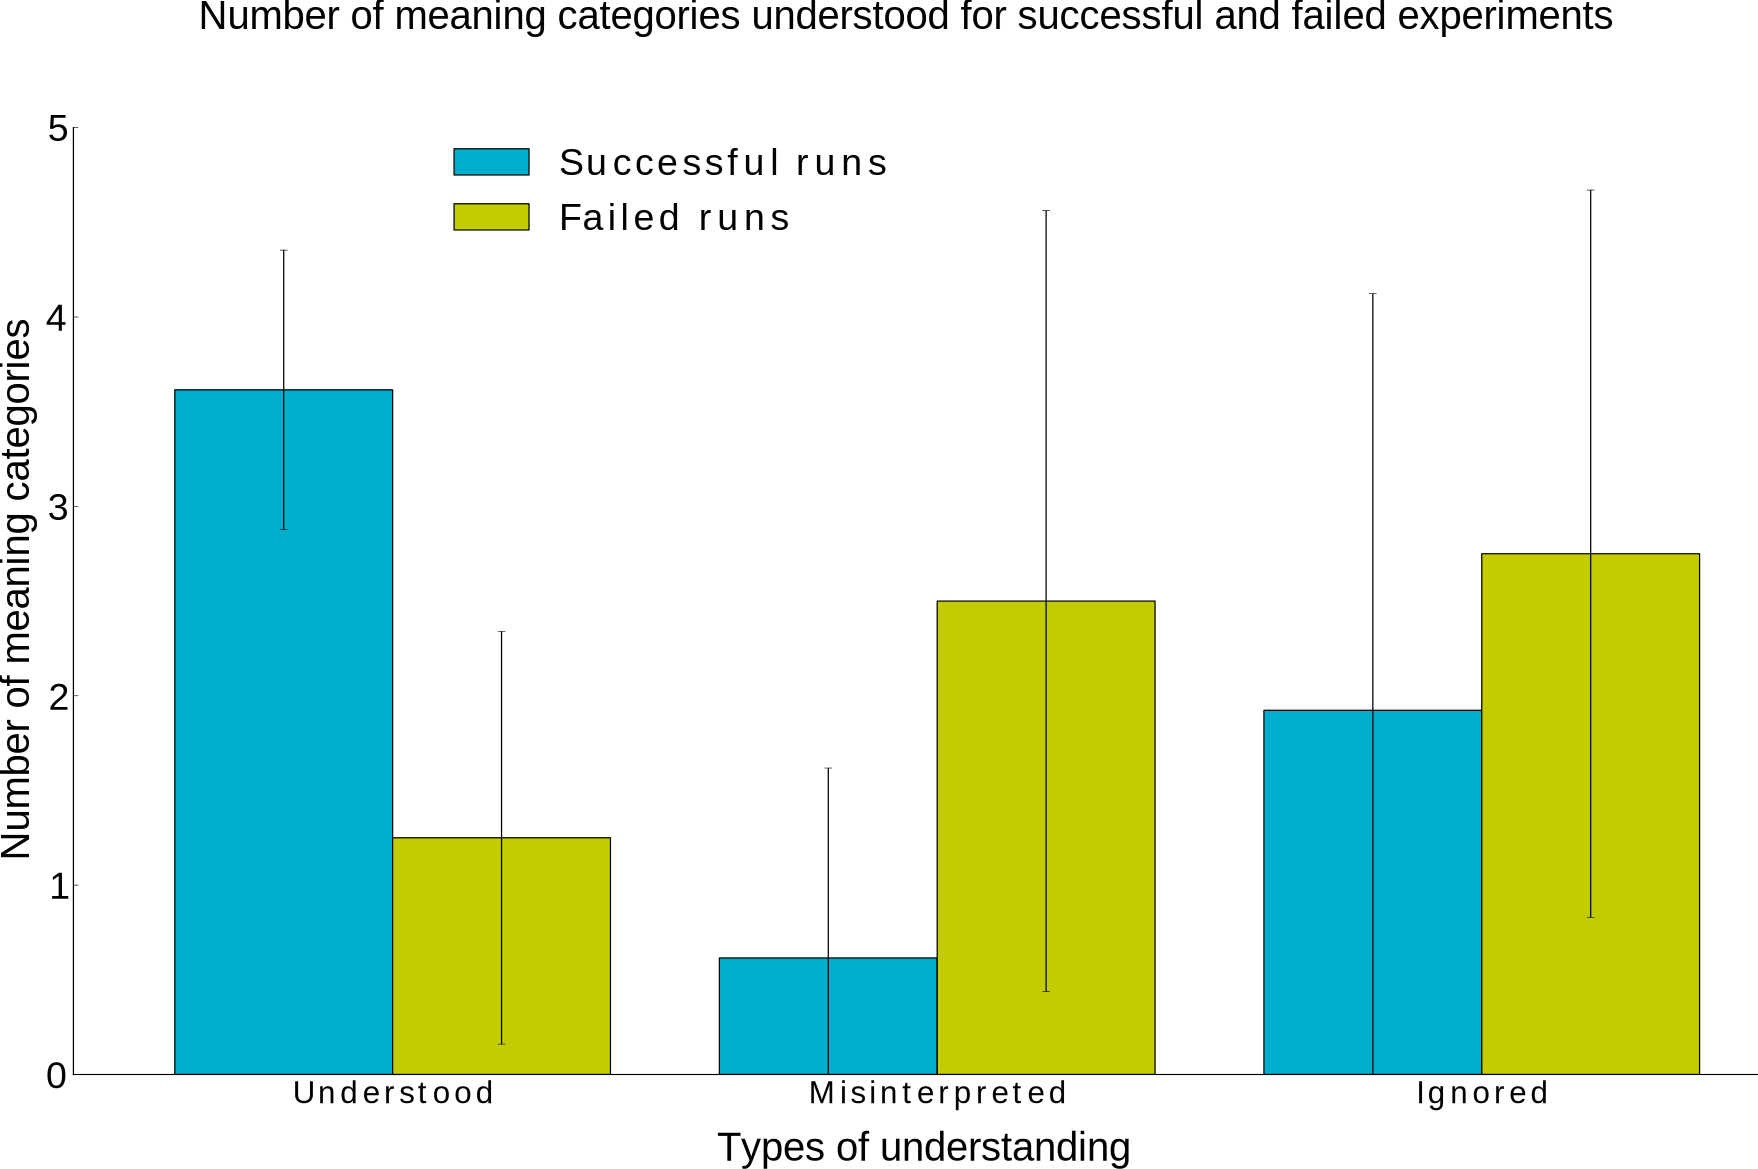
\includegraphics[width=\columnwidth]{\visualspdf/humanexp/meanings/understood_std.pdf}
        \caption{Distribution of meaning categories that were understood, misinterpreted, and ignored by the builders. Average across all builders for successful (blue) and failed (yellow) experiments.}
      \label{fig:types_of_understanding}
    \end{center}
\end{figure}

\begin{figure}[!htbp]
  \begin{center}
      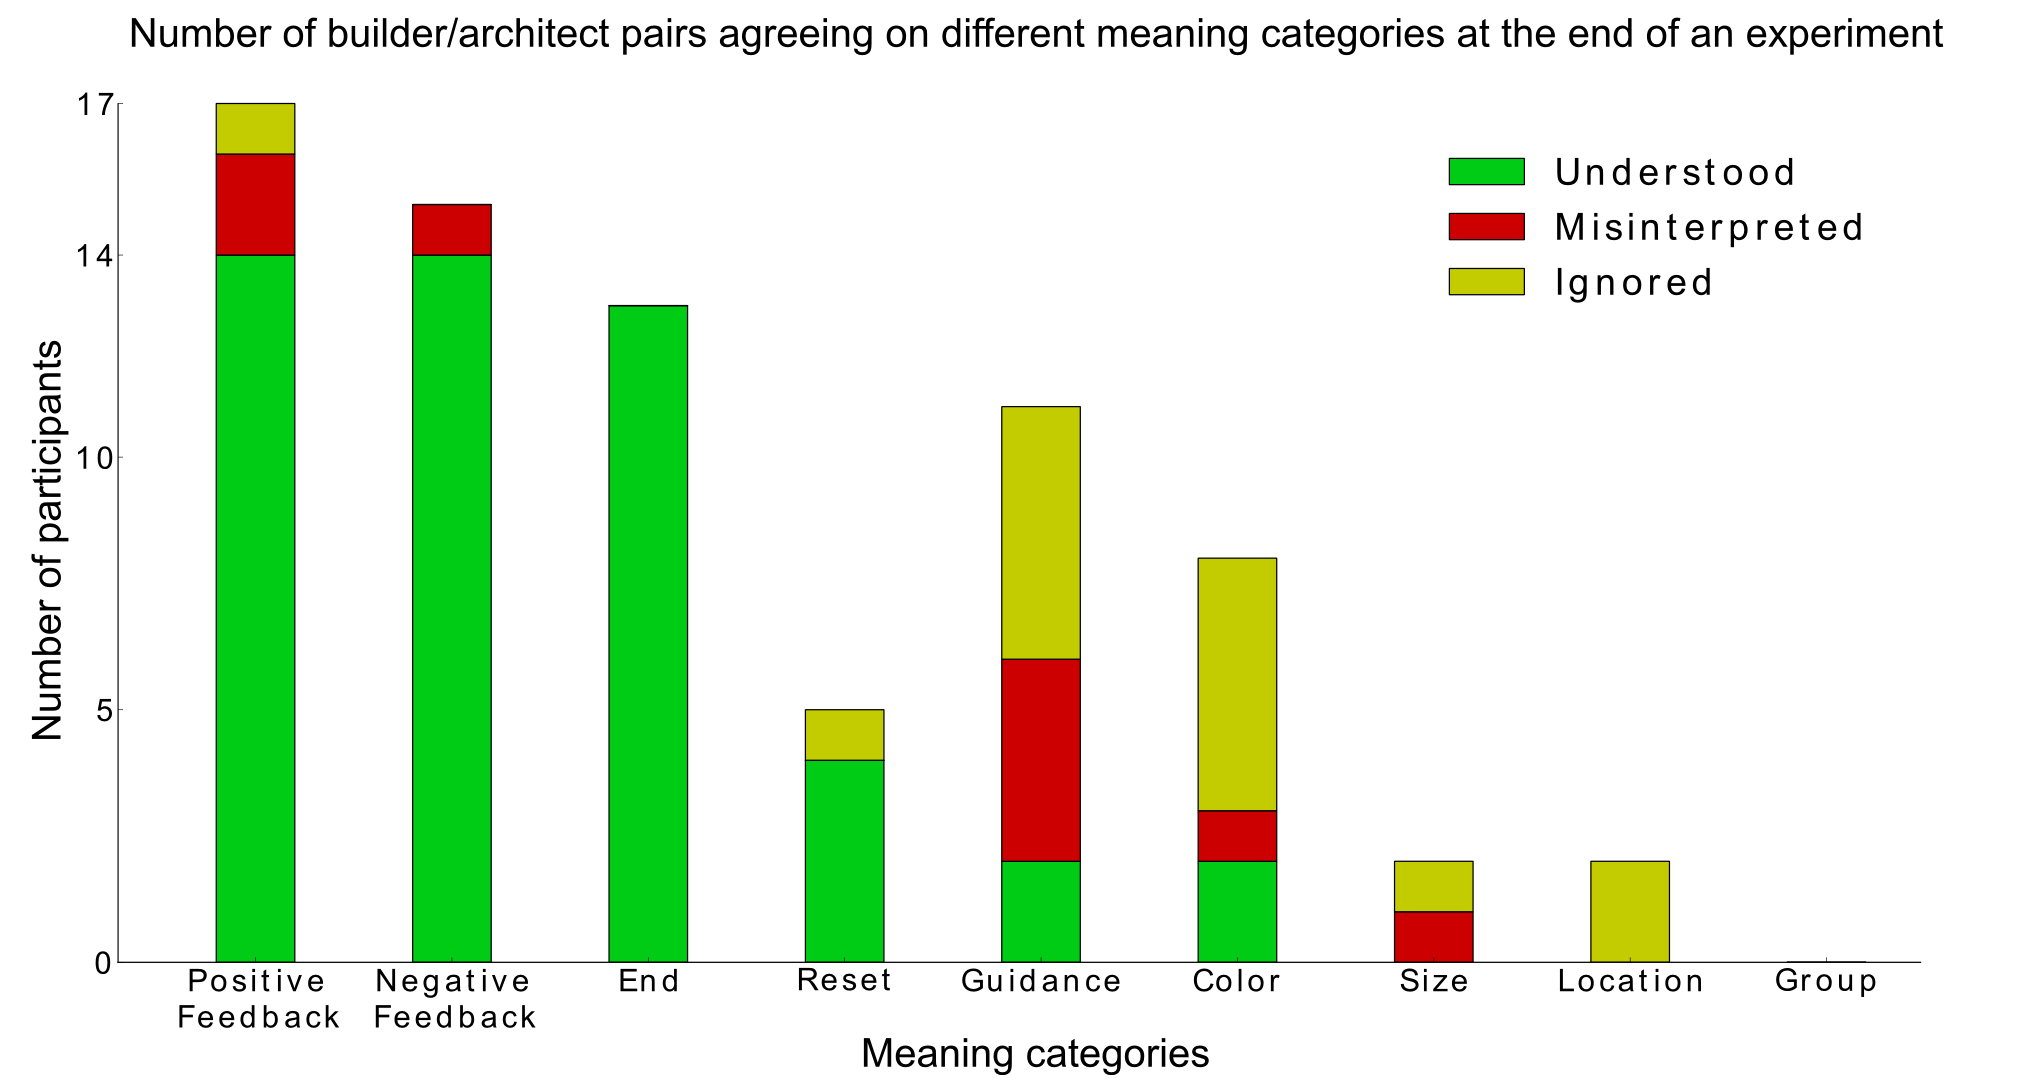
\includegraphics[width=\columnwidth]{\visualspdf/humanexp/meanings/instruction_understood.pdf}
      \caption{Number of builder/architect pairs agreeing or disagreeing on different meaning categories at the end of an experiment.}
    \label{fig:understanding_per_feedback}
    \end{center}
\end{figure}

It seems that even though many different signal meanings are initially considered by the architect, the players agree only on very few specific ones (positive feedback, negative feedback and End). The question of what are the main factors determining which meanings are considered by participants arises. This leads over to the next subsection in which we will consider the builder behavior to explore its role in which signal meanings are considered and in the ultimate outcome of the game.

\subsection{Builder Strategies}
\label{sec:builder}

For the builder, we aimed at identifying common actions across participants in an attempt to quantify the builders' strategies from the video data showing a top-down view of the workspace.
What follows is a description of observations on the builders' behaviors.

We identified two main strategies the builders embarked on (for an overview see Table~\ref{table:builder}). For these two strategies, the builders began by presenting only one block at a time. When they presented several blocks at once throughout the game, they did not seem to embark on a successful strategy.

The most common strategy for builders was to determine one correct brick at a time and to subsequently join it with the already assembled structure (see Figure~\ref{fig:timeline}). Figure~\ref{fig:timeline} is a case example of one game/run of the study in which this strategy is used successfully. The builders in $12$ (five first rounds and their five respective second rounds, one independent single first round, and one second round) of the $17$ runs pursued the same strategy. Only one game (a first round with a successful corresponding second round) of these $12$ failed.

The other strategy was to find all blocks belonging to the target structure. Blocks identified as correct were not joined right away, but in a first step all blocks belonging to the target structure were determined and were then subsequently joined one at a time in a second step. This strategy also involved the presentation of only one block at a time and was eventually pursued by two builders who both started out with a different strategy involving the presentation of multiple blocks. 

One builder initially tried to find which forms belonged to the target structure. Ultimately, he then identified all blocks belonging to the target structure by one at a time dividing all blocks into two groups. This builder played in a second round, for which in its corresponding first round multiple blocks were presented at a time by the builder and the game failed.

Another builder at the beginning tried to elicit a label for either color or form from the architect. In this case, all blocks of one specific color or of one specific shape were presented at a time. This strategy was only pursued by one builder at the beginning of the game, but was not successful and then therefore discontinued in favor of the strategy of finding which blocks belong to the target structure. This builder played in a first round. In the corresponding second round, the builder embarked on the first strategy.

The remaining three builders (in three first rounds) also presented multiple blocks at once but the set of blocks presented did not have any common properties and seemed random. These builders did not have any apparent systematic strategy and their games did not come to a successful end.

 \begin{table}[h]
 \begin{tabular}{p{0.22\columnwidth}|p{0.22\columnwidth}|p{0.12\columnwidth}|p{0.12\columnwidth}|p{0.06\columnwidth}}
%
 \multicolumn{1}{m{0.22\columnwidth}|}{\centering Presentation of blocks} & \multicolumn{1}{m{0.22\columnwidth}|}{\centering Strategy} & \multicolumn{1}{m{0.12\columnwidth}|}{\centering Number of games} & \multicolumn{1}{m{0.12\columnwidth}|}{\centering Successful} & \multicolumn{1}{m{0.06\columnwidth}}{\centering Failed} \\ \hline
%
 \multicolumn{1}{m{0.22\columnwidth}|}{\centering Present one block at a time} & \multicolumn{1}{m{0.22\columnwidth}|}{\centering Find one block and join right away, repeat}                    & \multicolumn{1}{m{0.12\columnwidth}|}{\centering 12}              & \multicolumn{1}{m{0.12\columnwidth}|}{\centering 11}                         & \multicolumn{1}{m{0.06\columnwidth}}{\centering 1}                      \\ \cline{2-5}
% 
  & \multicolumn{1}{m{0.22\columnwidth}|}{\centering Find all blocks belonging to the structure, then start joining} & \multicolumn{1}{m{0.12\columnwidth}|}{\centering 2}                       & \multicolumn{1}{m{0.12\columnwidth}|}{\centering 2}                          & \multicolumn{1}{m{0.06\columnwidth}}{\centering 0} \\ \hline 
 %
 \multicolumn{1}{m{0.22\columnwidth}|}{\centering Present multiple blocks at a time} & \multicolumn{1}{m{0.22\columnwidth}|}{\centering No strategy}                               & \multicolumn{1}{m{0.12\columnwidth}|}{\centering 3}               & \multicolumn{1}{m{0.12\columnwidth}|}{\centering 0}                          & \multicolumn{1}{m{0.06\columnwidth}}{\centering 3}                     
 \end{tabular}
 \caption{}
 \label{table:builder}
 \end{table}

Taking a closer look at the four failed experiments, we find that in one of them, where the builder presented one block at a time, in the end the target construction was almost finished. Architect and builder understood each other, but an early mistake in the position of one block was not signaled by the architect right away. He waited until the rest of the structure was completed and then tried to address the mistake by means of the introduction of a new signal. This new signal was interpreted by the builder as an \emph{End} signal, leading to the end of the game with one block in a position next to the target one. However for the other failed experiments, the structure at the end of the game was far from the target construction and there was no noticeable progress in all three cases.

Whereas, with the current data and analysis, we cannot yet draw any conclusions, still this observation suggests that the way the builders propose next steps and ask for information from the architect is important for the success of the game. Builders seem to build frames and create slots for the architect's input. These frames form the context which shapes the interpretation of the signals. This is similar to how in other cases of asymmetric or restricted communication, as for example in interactions with preverbal infants or in interactions with impaired persons, people provide frames to understand what their interaction partners with their different or limited conversational abilities want to communicate \cite{ochs1979propositions, goodwin1995co}.

\subsection{Additional Observations}

This subsection briefly indicates interesting, additional observations we made with our pilot study, as well as interesting considerations for future work.

First of all, we would like to state that the history of the interaction is crucial for understanding meanings. A person who has not witnessed the course of the interaction, is not able to fill in and complete the task without special instructions. We observe a phase of confusion and negotiation at the beginning of the interactions and after that a completion phase in which signal meanings have been constituted. The latter seems to be characterized by smooth, consistent patterns. In the initial phase of negotiation, we observed instances where the players adapted to their partners by changing the meaning of a button when they noticed the other player understands it differently (cf. Figure~\ref{fig:timeline} in Subsection~\ref{sec:case}). There were for example cases in which the meaning of buttons used to convey a positive or negative feedback reversed.

In contrast, we also observed that some players, both architects and builders, insisted on their strategies, even though the interaction with their respective partner did not work, i.e. they did not agree on any meaning and the task did not progress. Thus, there seem to be leaders and followers in terms of strategies, which could be personality-dependent, but could also manifest their ability to employ a theory of mind.

We also note that when builder and architect switched roles after a first round, their behaviors and performances were influenced (e.g., builder strategies were adopted across rounds). If a second round was systematically part of the experimental procedure, it would be interesting to see whether participants succeed faster in the second game they play with reversed roles and if they adopt similar strategies.

Another interesting aspect concerns timing, not only at which points in time the architect gives feedback and instructions, but also the interplay between the builder's and the architect's actions. The rhythm of the interaction partners' actions might be an important low-level feature in determining whether a certain signal means positive or negative feedback.

While the above points are highly relevant and worth investigating, their detailed examination is beyond the scope of this work.

\paragraph{Meaning switches and reset} 

During the experiment, we noticed some participants were misinterpreting a \emph{Positive feedback} as a \emph{Negative feedback} (and reversely), but most of the time they were able to detect and correct this misunderstanding. In few cases, it was the architect that inverted the meaning of the signals but in most cases it was the builder that had to reinterpret the signals, often after a \emph{Reset} instruction from the architect. The data we collected are not detailed enough for a fine-grained temporal analysis but we were able to count the number of feedback interpretation switches per run. In 5 out of 14 successful games (see Figure~\ref{fig:feedback_switch_enhanced}) the architect or the builder changed his use or interpretation of signals between positive and negative feedback.

\begin{figure}[!htbp]
  \begin{center}
      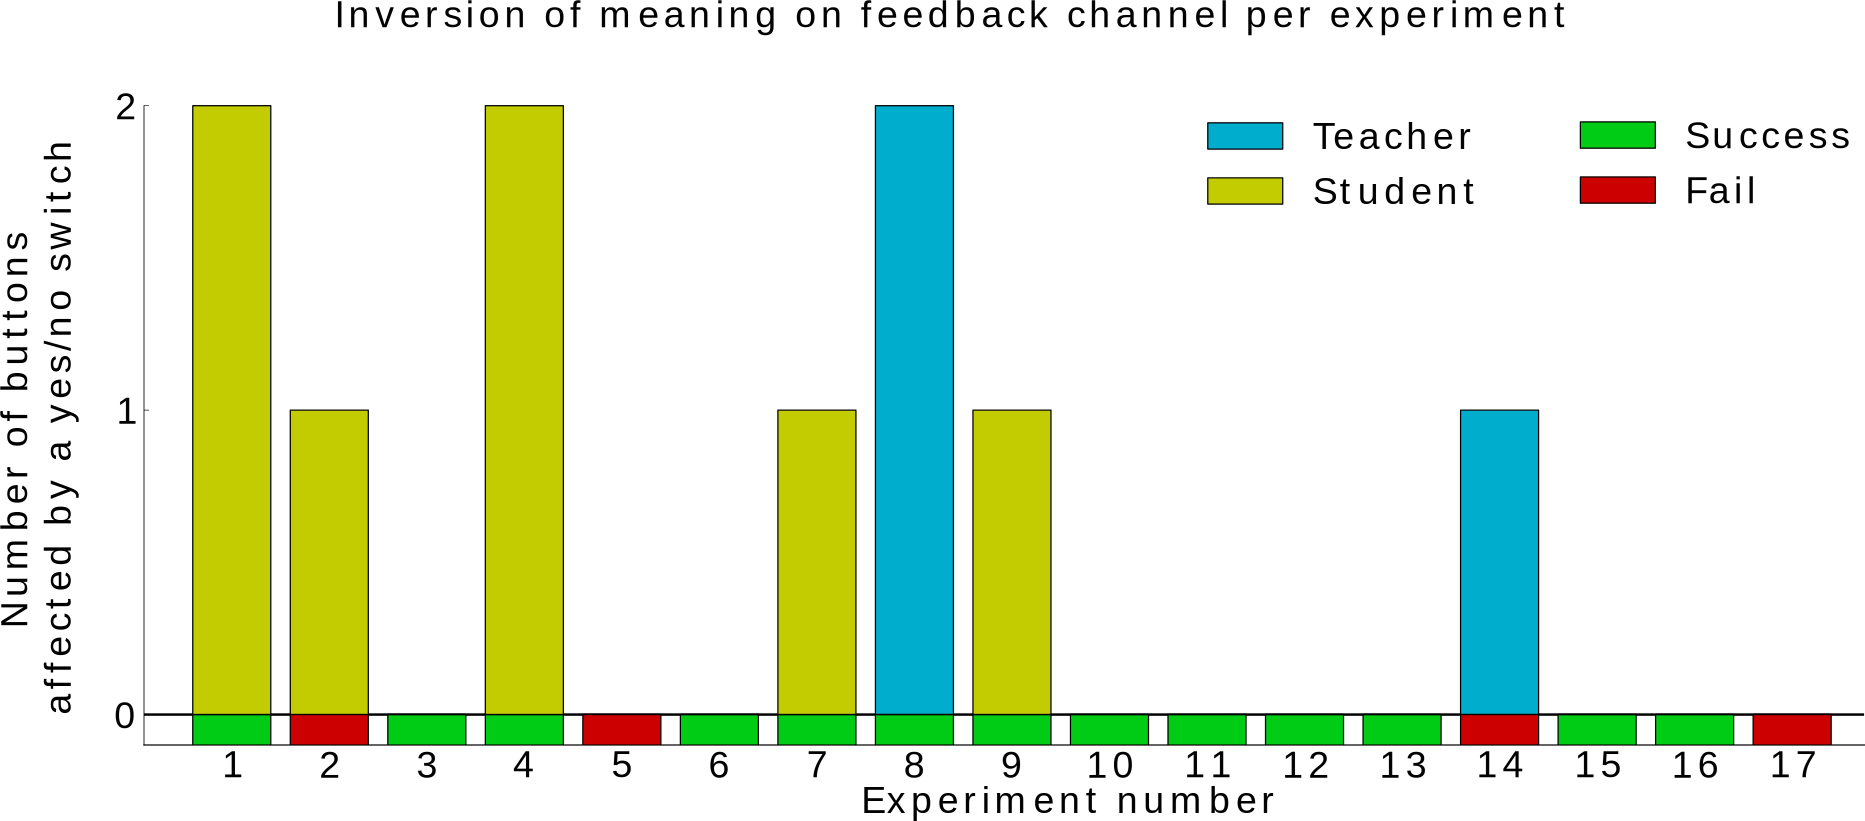
\includegraphics[width=\columnwidth]{\visualspdf/humanexp/meanings/inversion_meaning.pdf}
      \caption{Number of signals whose meanings switch between positive and negative feedback during the experiment. In blue, cases where the architect decides to change the meaning of a button from one feedback type to the other. In yellow, cases where the builder changes his/her interpretation of a signal. The colored bar on the bottom indicates if the experiment was successful or not.}
    \label{fig:feedback_switch_enhanced}
    \end{center}
\end{figure}


\paragraph{Context dependent meaning} 

In several cases the architect pressed all buttons to signify a salient event. This event was either perceived as a \emph{Reset} instruction if the builder felt lost or an \emph{End} instruction if the builder felt confident about his/her understanding of the previous interaction sequences. This is illustrated in figure~\ref{fig:timeline}, where at $t=200 s$, as players already tried for several iteration with no success, the architect presses all buttons to signify a \emph{Reset}. After this \emph{Reset}, a new set of symbols is used by the architect which is well understood. Finally, to signify that the construction is finished, the architect presses again all buttons simultaneously now with the intended meaning that the task is completed. As the interaction was going well, this signal was understood as a \emph{End} signal by the builder and the experiment goes to a successful end.

As detailed earlier one of the experiment failed even if the in the end the target construction was almost finished. Architect and builder understood each other, but an early mistake in the position of one block was not signaled by the architect right away. He waited until the rest of the structure was completed and then tried to address the mistake by means of the introduction of a new signal. Given the context (the interaction was smooth and participants understood each other), the introduction of this new signal was interpreted by the builder as an \emph{End} signal, leading to the end of the game with one block in a position next to the target one.

\paragraph{Timing} 

Figure~\ref{fig:timeline} contains information on which signal the architect sends to the builder at which point in time as well at its alignment with the construction progress. Such information allow to analyse individuals' temporal coordination during social interactions, i.e. the timing and interplay of interaction at both a micro and macro scale \cite{delaherche2012interpersonal}.

\paragraph{Confirmation bias} 

Some builders were affected by the confirmation bias which is defined as \textit{``the seeking or interpreting of evidence in ways that are partial to existing beliefs, expectations, or a hypothesis in hand''} \cite{nickerson1998confirmation}. While mistaking negative feedback for positive feedback, participants were progressing far in a wrong direction, even if the signal would seem contradictory for an outside observer. It was difficult for some users to re-assess their belief, they better thought the architect was mistaking or were pursuing in a very improbable direction. Few builders were able to overcome the confirmation bias problem by themselves, leading either to a failed experiment or needed the architect to produce a salient event to reset the experiment. With the recorded data, it is unfortunately not possible to quantify this phenomenon even if the figure~\ref{fig:feedback_switch_enhanced} may provide useful information.

\paragraph{Workspace} 

From our video recording, we observed that some builders (9 out of 17) cleaned their workspace in the beginning of the experiment, such that no block is remains visible. They then tried to maintain a clean workspace during the game, giving them a presentation space, where they could propose blocks in an unambiguous way. Another strategy was pursued by eight builders who from the beginning kept all blocks on the workspace and therewith enabled the architect to witness the process of choice of block. Of these eight builders, three neatly ordered and aligned their blocks on the workspace and proposed one block at a time by pointing to it. The remaining five builders did not order or align the blocks in any way. These participants opened up a workspace inside the overall workspace (i.e., proposing blocks in-between or next to the rest).

% \begin{itemize}
% \item clean workspace used as presentation space (9)
% \item all blocks in view (8) (nicely aligned (3), or not aligned (5))
% \end{itemize}

\paragraph{Propositions} 

Essentially the task consisted in two subtasks, finding correct blocks and joining them. For this, participants proposed blocks and positions of blocks in different ways. For proposing blocks in search for a correct one, builders ``present'' blocks by placing them alone on the workspace or in a separate sub-workspace, they point to the block they wish to receive feedback about, or they lift the respective block to highlight it.

% \begin{itemize}
% \item present
% \item point
% \item lift
% \end{itemize}

To find at which position a specific block is correctly joined with others, the propositions differ in the level of accuracy and precision of the proposed position. Some builders begin with bumping two blocks together to receive feedback about if they should be joined at all. In some cases the respective block is placed above, below, on the right or on the left of a structure to receive course feedback about the location of the correct position. Another way of presentation is to continuously move the respective block around the structure with expected positive feedback when the correct position is reached. Some builders discretely test or propose positions on the way around the structure by only pausing, joining blocks half way, or fully joining the blocks at each possible position.

% \begin{itemize}
% \item bump
% \item order (bottom to top)
% \item right, left, above, below
% \item continuously move around the structure
% \item discretely stop at each position or join half-way
% \item join at each possible position
% \end{itemize}

%%%%%%%%%%%%%%%%%%%%%%%%%%%%%%%%%%%%%%%%%%%%%%
%%%%%%%%%%%%%%%%%%%%%%%%%%%%%%%%%%%%%%%%%%%%%%
%%%%%%%%%%%%%%%%%%%%%%%%%%%%%%%%%%%%%%%%%%%%%%
%%%%%%%%%%%%%%%%%%%%%%%%%%%%%%%%%%%%%%%%%%%%%%
%%%%%%%%%%%%%%%%%%%%%%%%%%%%%%%%%%%%%%%%%%%%%%
\section{Lessons Learned}

We presented a new experimental method that allows studying important aspects of human communication with high relevance to human-robot interaction. We show that two players that never had a chance to interact by the means of a restricted interface before were able to communicate and act upon communicative acts whose meanings were never explicitly negotiated between interaction partners. What can we learn from the experiments? How can it be used for human-robot interaction?

We first link our experiment with the concept of interaction frame defined in introduction (chapter~\ref{chapter:introduction}). We then describe the main strategy used by our participants. We highlight the active role of the builder in creating slots for the architect to provide information. And further identify the main strategy used to learn the meanings of button presses, which consist of generating interpretation hypothesis and trying to validate or discard them through further interactions. 

% Finally, and based on those observations, we start defining the problem of learning from unlabeled interaction frame in more concrete terms.

\subsection{Use of interaction frames}
\label{chapter:humanexperiment:frames}

The experimental setup setup described above is less constrained than our challenge of \emph{learning fro unlabeled interaction frames} defined previously. As a reminder this problem assume the interaction frames associated to the interaction between the robot and the human is known and only the mapping between teaching signals and their meanings is unknown. Knowing the interaction frame means having access to: \begin{inparaenum}[(a)] \item the set of possible meanings the teacher can refer to, \item the details and timing of the interaction, and \item the constraints that apply on the possible tasks. \end{inparaenum}

In the human-human experiment described in this chapter, the interaction frame is not defined in advance. The meanings associated to the button events are not constrained to belong to a finite set, and the details and timing of the interaction, i.e. the protocol, are also undefined at start. Only the context in which the interaction takes place is provided to both participants, which is to build a flat construction that does not necessarily contain all available blocks.

The first interesting fact is that, while all of participants thought the problem impossible to solve, most of them were able to successfully cooperate under restricted and asymmetric interaction.

The second interesting fact is that users seemed to rely on ``usual'' interaction frames to make sense of the interaction (cf figure~\ref{fig:types_of_feedback}). Especially, participants came up with strategies involving both the details and timing of the interaction and the possible meanings associated to the button events. In the next two subsections, we will highlight the following observations: 

\begin{itemize}

\item The timing and alignment of the interaction between both participants quickly converged. Especially the builder seemed to be the leader in the construction of the interaction protocol. With his/her propositions of blocks and positions, the builder provides frames in which he/she creates slots for the architect to provide information.

\item The architects and the builders considered only a limited number of meaning types; among which only positive and negative feedback was considered by all participants. Builders seem to rely on the assumption that the signal observed would belong to one of these categories. They then relied on interpretation hypothesis with respect to both the task (i.e. the possible constructions) and the meaning of the signals. By testing several combination of task and signal's meaning, the builder was able to identify the correct signal to meaning mapping, most often leading to a success in the construction task.

\end{itemize}

\subsection{Slots of interaction}

Signals' meanings are co-constructed by the interaction partners, but the builder's actions seem to play a key role in structuring the interaction. With his/her propositions of blocks and positions, the builder provides frames in which he/she creates slots for the architect to provide information. And thus the builder's created frames constrain the meaning of the architect's input to a large extent. 

For example, by cleaning the workspace of all blocks and presenting new blocks one at a time, the builder influences the architect to provide a signal whose meaning can be: ``this block belongs/does not belong to the construction'' or ``this block is blue/red/yellow'' for example. This way the builder additionally imposes the timing of the interaction, e.g. a turn taking social behavior where the builders propose a new block and waits for a signal from the architect. As a result, the builders is now faced with a similar problem than our problem of \emph{learning from unlabeled interaction frames}, where the meanings are limited to a finite set, known from both partners. The frame created by the builder also defines the association between world's event (e.g. movement of cubes) and instruction signals. However the particular meaning of the button presses inside each frame is still to identify, e.g. whether the observed signal means the block belongs or does not belong to the final structure.

This behavior has also been observed in other asymmetric and restricted interactions involving interaction partners with limited communicational abilities, as for example preverbal infants or impaired persons \cite{ochs1979propositions, goodwin1995co}. 

Therefore, it might be interesting to consider similar mechanisms of proposition in a learning robot as means to elicit appropriate signals from a human tutor in HRI \cite{cakmak2012designing,vollmer2014robots,cangelosi2010integration}, especially if the interaction protocol is not explicitly define in advance. These interesting directions are not the subjects of this thesis, and in our experiments we will assume the human teacher is aware of the interaction frame. It is only in chapter~\ref{chapter:limitations:framehypothesis} that we soften this assumption, assuming a finite set of possible interaction frames is available.

\subsection{Interpretation hypothesis}
\label{chapter:humanexperiment:interpretationhypothesis}

Humans are capable of solving the kind of communication problem robots can encounter with humans. We have observed that both builders and architects have preconceptions of what interaction frames the other player is likely to understand, trying to use or interpret signals with respect to those frames. With the ``feedback frame'' the most commonly thought about and the easiest to understand in the context of our experiment. And with \emph{Reset} and \emph{End} instructions being more frequently considered than guidance, color, or size related instructions.

To solve the restricted asymmetric interaction problem arising from our experimental setup, participants projected the ongoing interaction into those different common interaction frames. They were creating interpretation hypothesis of the signals and behaviors of each other, which were later discarded or validated in light of the next observations. Especially, a hypothesis is retained if its predictions are more coherent with the history of interaction.

For example, let's consider you are the builder and you present only two blocks on the workspace to be visible to the architect. You then test one by one every possible stacking combination with these two cubes. Between each test you wait few seconds to observe the signal from the architect. Given your behavior, you expect to elicit a yes/no type of signal from the architect and will start hypothesizing the signals you receive belong to this category.

Therefore, after having tried all possible stacking combination of blocks, you expect only two possible outcomes. The first possibility is that you received the same, unique, signal all along, and you may assume that the two blocks selected do not stack together in the final construction. In addition you could also assume that the signal you observed mean your actions were ``incorrect''. The other possibility is that you observed two different signals, with one being way more frequent than the other. In such case, you may hypothesize that the less frequent signal corresponds to an ``incorrect'' meaning. Indeed, given the construction task, there should be more incorrect possible stacking than correct stacking. Therefore the other signal should mean ``correct'', and the associated stacking of block should be part of the current structure. In that case, you can stack the block together and try to introduce a new block, that time knowing what signal means ``correct'' and what signal mean ``incorrect''.

But things are not that easy. The architect might not have understood your behavior or the fact you asked for a yes/no type of instruction. It might have send always the same signal but asking you to take a new block. In that case, given your hypothesis, you might believe this signal means ``incorrect'' instead of meaning ``pick a new block''. But the architect may also have tried to guide your movement towards the correct position (using ``above'', ``under'', ``to the left'', or ``to the right'' instructions), in such case you should have noticed that you received more than two different signals and would have to reconsider your hypothesis.

Therefore it might be useful to check if the behavior of the architect could not belong to another interaction frame. You might try to find a situation allowing differentiating between the remaining hypothesis. And after a more of less lengthly procedure, you might end up being sure of the architect intended meanings and succeed in the construction task.

As a final note, on top of all these hypotheses, you cannot assume the architect behavior is constant through time because he also tries to adapt to your behavior. This makes our human-human experiments way more complex than the problem considered in this thesis, where we consider the teaching behaviors of our users are constant through time.

The example we provided is well illustrated by the first four minutes of interaction of the experiment presented in Figure~\ref{fig:timeline}. We can observe that, during these four minutes, both the builder and the architect change frequently their use and interpretation of the signals. After a \emph{Reset} event is sent by the architect, the interaction starts again on a more structured interaction, which finally led both participants to agree on a communication system and to succeed at the co-construction task.

\transition

Based on our observations, we can aim at constructing robots capable of learning a task from human instructions without programming them in advance to understand the human communicative signals. To do so, we should inform the robot about the interaction frame, which indicates: \begin{inparaenum}[(a)] \item the set of possible meanings conveyed by the teacher (e.g. the teacher use only positive and negative feedback), \item the details and timing of the interaction (such as to map teaching signals to world events), and \item some constraints on the possible tasks (such as to limit the search space of the robot). \end{inparaenum}. Given this information, by making hypothesis on the task, the user can generate interpretation hypothesis of every users' communicative signal according to each hypothesized task. As the teacher only follows one of the task, the hypothesis from which emerges a better coherence between the interaction history, the interaction frame, and the task, is likely to be the one the teacher as in mind. We formalize this idea in next chapter and provide simple visual examples of both the problem and the properties we exploit to solve it.




% %!TEX root = ../../thesis.tex
\define{\chapterpath}{\allchapterspath/lfui}
\define{\imgpath}{\chapterpath/img}

\chapter{Learning from Unlabeled Interaction Frames}
\label{chapter:lfui}
\minitoc

\blfootnote{The work presented in this chapter has been published in \cite{grizou2013robot}. Code is available online under the github account \url{https://github.com/jgrizou/} in the following repositories: \href{https://github.com/jgrizou/lfui.git}{lfui}, \href{https://github.com/jgrizou/experiments_thesis.git}{experiments\_thesis}, and \href{https://github.com/jgrizou/datasets.git}{datasets}.}

We identified a potential mechanism for robots to learn a new task from human instructions without programming them in advance to understand the human instructions signals. This mechanism is based on the generation of interpretation hypothesis of the teaching signals with respect to specific constraints from the task and the interaction frame. It hypothesizes that the correct hypothesis will explain better the history of interaction.

In this chapter, we exemplify the problem in a simple seven discrete states world, remind the underlying assumptions and define the notation used. We illustrate the interpretation hypothesis mechanism on our visual example and, based on our observation, we define the metric our algorithm will rely on. We then apply our algorithm to a pick and place scenario using a six degrees of freedom robot and speech utterances as the modality of interaction. We show that our algorithm is able to identify a task in less than on hundred iterations when the teacher is providing feedback signals whose mapping to their associated meaning in a priori unknown. We further show that the system is robust to some teaching mistakes and that the knowledge learned during a first experiment can be reused for learning a second task faster. Finally, we will show that two different simple action selection methods for our robot lead to differences in learning efficiency. This observation opens the question of how our robot can plan its action to improve its learning performances, which will be investigated in next chapter.

%%%%%%%%%%%%%%%%%%%%%%%%%%%%%%%%%%%%%%%%%%%%%%
%%%%%%%%%%%%%%%%%%%%%%%%%%%%%%%%%%%%%%%%%%%%%%
%%%%%%%%%%%%%%%%%%%%%%%%%%%%%%%%%%%%%%%%%%%%%%
%%%%%%%%%%%%%%%%%%%%%%%%%%%%%%%%%%%%%%%%%%%%%%
%%%%%%%%%%%%%%%%%%%%%%%%%%%%%%%%%%%%%%%%%%%%%%
\section{Problem formulation}

In chapter~\ref{chapter:introduction}, we defined the problem of \emph{learning from unlabeled interaction frames}. In short, a human instruct a robot to perform a task by providing it instructions through communicative signals. The problem is that the robot does not know the task, neither the mapping between the teacher' signals and their meanings. The robot is not teleoperated but rather decide by itself which actions to perform. The task is sequential which means the robot should perform a sequence of multiple actions to fulfill it. We exemplify with the following example.

\subsection{Example of the problem}
\label{chapter:lfui:example}

We present a T world example (see Figure~\ref{fig:Tworld}) that will follow us during the remaining of this thesis. In this example, an agent lives in a discrete seven states world that has a T shape. The agent can perform four different actions (go left, right, up ,and down).

\begin{figure}[!htbp]
  \centering
  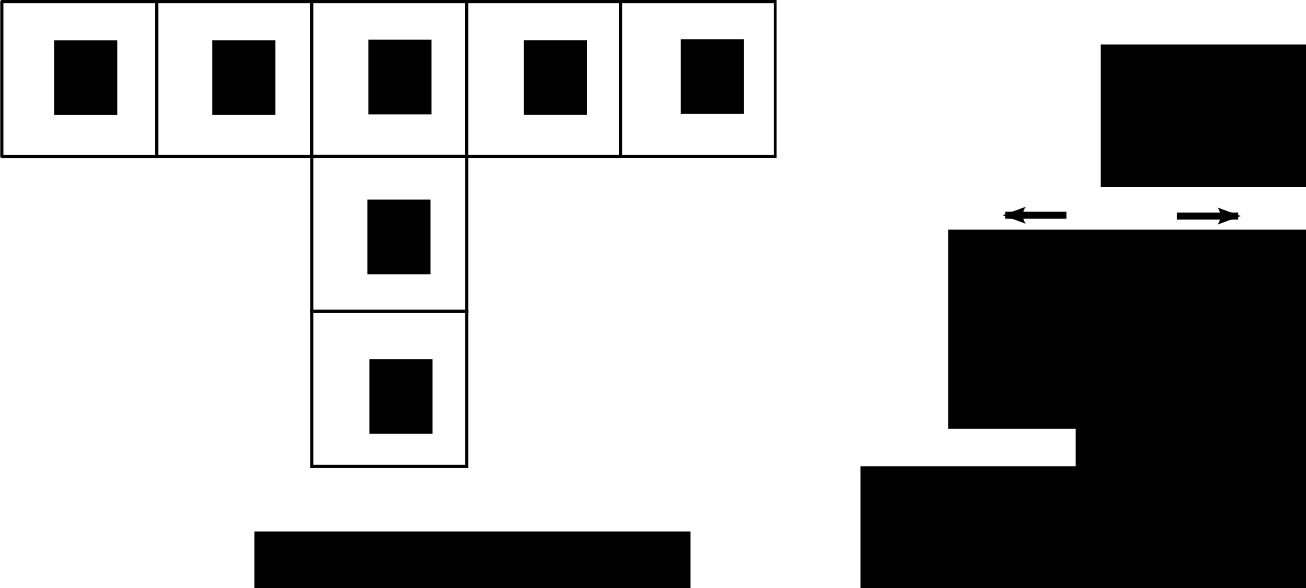
\includegraphics[width=\tworldsize\columnwidth]{\visualspdf/worlds_and_datasets/Tworld_with_state_number_and_action.pdf}
  \caption{The T world and the available actions.}
  \label{fig:Tworld}
\end{figure}

A simulated teacher wants the robot to reach, and stay at, the left edge of the T world (i.e. state 1). To this end, the teacher provides feedback information to the robot. Feedback signals are represented as two dimensional feature vectors and can have two different meanings: ``correct'' or ``incorrect''. As depicted in Figure~\ref{fig:feedbacksignals}, we assume these signals are randomly generated by two multivariate normal distributions, one for each meaning. We associate green and red colors respectively to signals of ``correct'' and ``incorrect'' meanings. When the teacher wants to send a feedback of meaning ``correct'', he samples a signal from the right, green, Gaussian. Respectively, a signal of meaning ``incorrect'' will be generated on the left side of the feature space. These signals are represented in a two dimensional feature space, which could represent any modality used by the teacher to communicate with the robot, such as speech, gestures, facial expression, or even brain signals.

\begin{figure}[!htbp]
  \centering
  \includegraphics[width=\signalwidth\columnwidth]{\visualspdf/worlds_and_datasets/feedback_signals_color.pdf}
  \caption{The feedback signals used in our visual examples. A signal of meaning ``correct'' will be generated on the right side of the feature space, and a signal of meaning ``incorrect'' will be generated on the left side. Importantly, the agent will never have access to the label information, represented by the color of each signal.}
  \label{fig:feedbacksignals}
\end{figure}

The interaction between the agent and the teacher is turn-taking. First, the agent, which is in a particular state, performs one action and transitions to its next state. The teacher is observing the robot and evaluates the robot's actions with respect to the task he has in mind (i.e. the robot should go and stay in state 1). The teacher then sends the corresponding signal to the robot. However, the robot neither has access to the task the user has in mind, nor it has access to the meaning of the signal sent by the teacher. For the sake of the example, we assume that there are only two possible tasks, reaching G1 or G2.

For example, as depicted in Figure~\ref{fig:TworldOneStepUnlabeled}, the agent starts in state 3, performs action left, and ends-up in state 2. The teacher wants the agent to go to G1, therefore he sends a signal of meaning ``correct'' (i.e. in the right part of the feature space). Note that the signal shown in Figure~\ref{fig:TworldOneStepUnlabeled} (left) is neither green nor red, its label is undefined.

\visuopti{\vspace{-0.3cm}}

\begin{figure}[!htbp]
  \centering
  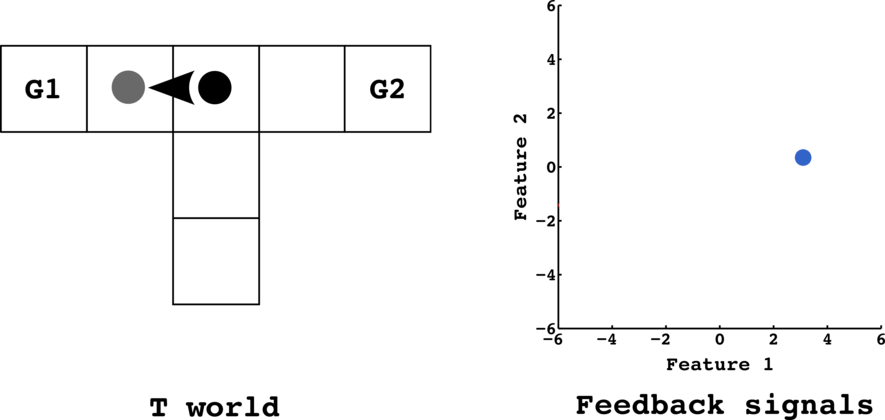
\includegraphics[width=\tworldsize\columnwidth]{\visualspdf/tuto_feedback/Tworld_feedback_unlabeled_one_action.pdf}
  \caption{The teacher provides a feedback signal after each action of the agent. The agent starts in state 3, performs action left, and ends-up in state 2. The teacher wants the agent to go to G1, therefore he sends a signal meaning that the previous action was ``correct'' with respect to the goal. The signal is on the right side of the space as described in Figure~\ref{fig:feedbacksignals}. However the agent does not have access to the label associated to this signal, it only observes a point in a two dimensional space.}
  \label{fig:TworldOneStepUnlabeled}
\end{figure}

After performing several actions randomly, the robot ends-up with a lot of observations associating a state, an action and a feedback signal. As depicted in Figure~\ref{fig:TworldManyStepUnlabeled}, we can observe that two clusters have emerged in the feature space. A straightforward assumption is that one cluster is associated to the ``correct'' meaning, and the other to the ``incorrect'' meaning. We will see how this assumption of consistency in the signals can be exploited in the coming sections.

\visuopti{\vspace{-0.2cm}}

\begin{figure}[!htbp]
  \centering
  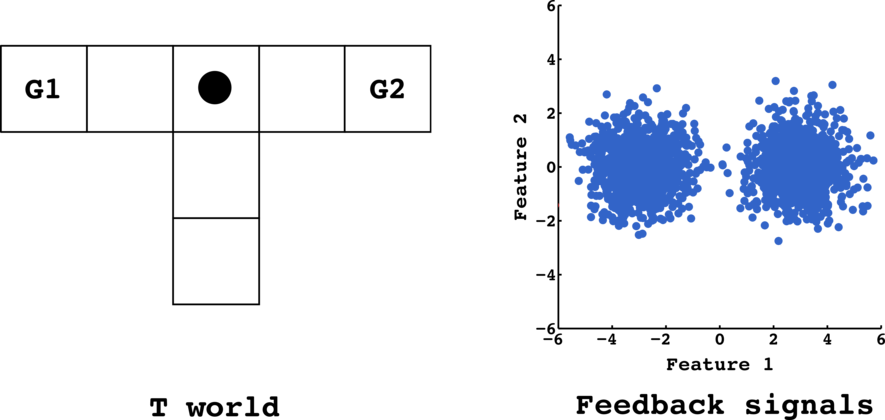
\includegraphics[width=\tworldsize\columnwidth]{\visualspdf/tuto_feedback/Tworld_feedback_unlabeled.pdf}
  \caption{After performing several random actions, the robot ends-up with many of observation associating a state, an action and a feedback signal.}
  \label{fig:TworldManyStepUnlabeled}
\end{figure}

\subsection{What the agent knows}

The problem described in this section is impossible to solve without further information. Indeed, even if the agent was able to identify the two clusters, it does not have access to the meaning associated with each cluster. In practice it would be easier if the robot had access to the mapping between teaching signals and their meanings. A typical solution is therefore to rely on a phase of calibration, where the system is given signal-meaning pairs and learns the mapping using a supervised learning algorithm. Given this information, in our example of Figure~\ref{fig:TworldOneStepUnlabeled}, it becomes trivial to identify the task. Starting in state 3, if the robot does action ``left'', it ends up in state 2, and if it receives a signal of meaning ``correct'', then the correct task is to reach the left edge of the T marked by G1.

As mentioned before, in this work the robot cannot rely on the phase of calibration. However the robot has access to the interaction frame, which provides theoretical information about the human teaching behavior. The robot knows:
\begin{itemize}

\item \textbf{Details and timing of the interaction.} After each action, the robot waits for a signal from the teacher. This signal provides information related with the action the robot just performed.

\item \textbf{The set of possible meanings the human can refer to.} The teacher assesses the last action of the robot with respect to an unknown task. The signals' meanings can be ``correct'' or ``incorrect''.

\item \textbf{Constraints on the possible tasks.} There are only two possible tasks, reaching the left (G1) or the right (G2) edge of the T world.

\end{itemize}

In addition the robot has access to the $Frame(Context,Task)$ function that, given a context of interaction and a task, returns the meaning intended by the teacher. For example, the robot knows that if it moves from state 3 to state 2, and that the human wants it to go in G1, then the signals received from the human means ``correct''.
%
\begin{eqnarray}
``correct" = Frame((s3 \rightarrow s2), G1) \nonumber
\end{eqnarray}
%
Respectively, if the robot moves from state 3 to state 2, and that the human wants it to go in G2, then the signals received from the human means ``incorrect''.
%
\begin{eqnarray}
``incorrect" = Frame((s3 \rightarrow s2), G2) \nonumber
\end{eqnarray}

% \subsection{Learning from unlabeled interaction frame}

% In previous chapter~\ref{chapter:humanexperiment:frames}, we defined the terms of interaction frames which represents a stereotyped situations, a schema of interpretation given a particular situation or event. Such frame is often assumed to be known by both the human and the robot in addition to the signal-to-meaning classifier that translates the actual human signals into meaningful symbols. By comparing what the frame predicts and what the human actually said the robot can change our understanding of the situation.

% Learning from unlabeled interaction frames correspond to the problem where the signal-to-meaning classifier is not given, and therefore the robot can not rely on a direct comparison between the prediction from the interaction frame and the observation from the human teacher.

% What remains is the frame. It is at the core of our approach, it is assumed to be known by both the human and the robot. It includes both the constraints related to the task, e.g. teaching a robot which state to reach among a finite set of states, and the protocol used by the teacher to communicate to the robot, e.g. the teacher is assessing the robot's actions. Therefore, the meanings of the unlabeled signals are not explicitly given but are known to belong to a finite set of possible meanings.

% We define a generic frame function that, given a context of interaction and a task, returns the meaning intended by the teacher:
% %
% \begin{eqnarray}
% Meaning = Frame(Context, Task)
% \end{eqnarray}
% %
% Following our previous example, stating that if the robot moves from state 3 to state 4 (context), and that the human wants it to go in G1 (task), then the signals received from the human means ``incorrect'' (meaning), we can exemplify the use of the frame:
% %
% \begin{eqnarray}
% ``incorrect" = Frame((s3 \rightarrow s4), G1)
% \end{eqnarray}

% \transition

% The idea of unlabeled interaction frame summarizes the problem of interaction we tackle in this work. However it is a quite general concept, and in order to understand the underlying principles of our algorithm, in the following sections we will restrict our analysis to simple frames and simple worlds. We will also explicit a number of assumptions related to this work.


%%%%%%%%%%%%%%%%%%%%%%%%%%%%%%%%%%%%%%%%%%%%%%
%%%%%%%%%%%%%%%%%%%%%%%%%%%%%%%%%%%%%%%%%%%%%%
%%%%%%%%%%%%%%%%%%%%%%%%%%%%%%%%%%%%%%%%%%%%%%
%%%%%%%%%%%%%%%%%%%%%%%%%%%%%%%%%%%%%%%%%%%%%%
%%%%%%%%%%%%%%%%%%%%%%%%%%%%%%%%%%%%%%%%%%%%%%
\section{What do we exploit}

% Following our T world example, the robot knows the world, the effect of it actions. The robot also knows the human wants it to reach one of the two edges of the T world marked with G1 and G2. The robot is also aware of the interaction frame, in our case that the teacher will provide, for each action performed by the robot, a feedback signal meaning either ``correct'' or ``incorrect''. The robot further knows how the teacher should behave with respect to one particular goal.
% Central to our method is a system of hypothesis. 

Following our T world example, we now present a visual representation of the interpretation hypothesis mechanism. From the observation made in chapter~\ref{chapter:humanexperiment:interpretationhypothesis}, the robot will generate interpretation hypothesis of the signals with respect to all possible tasks. For a particular task hypothesis, the robot will assign hypothetic meanings, or labels, to the human signals according to its previous actions and knowing the meanings are either ``correct'' or ``incorrect''. The system is ``reasoning'' as follow: \textit{``If the human wants me to solve task G1, then when I performed action ``left'' in state $3$, its feedback signal should mean ``correct'' ''}. For the sake of our example, we only consider two hypothesis, G1 and G2, as depicted in Figure~\ref{fig:TworldManyStepUnlabeled}.

% We exemplify the idea of interpretation hypothesis following our T world example in section~\ref{chapter:lfui:example}. 

\subsection{Interpretation hypothesis}
\label{chapter:lfui:interpreation}

% We considerer the same interaction as in section~\ref{chapter:lfui:example}. 

% For the sake of the example and ease of explanation, we consider those two-dimensional signals as representing speech utterances.

For each action, the robot receives raw unlabeled two dimensional signals. Following the above explanation, for a particular hypothesis (G1 or G2), the robot can assign hypothetic meanings to the human signals knowing they are limited to a finite set and according to the interaction history. We assume our teacher is optimal and therefore assume our agent is aware of the optimal policies for each task  (see Figure~\ref{fig:Twolrdpolicies}), which can be used to interpret the human signals.

% The machine is ``reasoning'' as follow: \emph{"If the human wants me to solve task G1 then when I performed action $a$ in state $a$ and he said ``oui'', he meant ``incorrect''"}. 

% We exemplify this process using the same example as in Figure~\ref{fig:TworldOneStepUnlabeled} and according to our two task hypothesis which are reaching either of the two edges marked as G1 or G2. 

\begin{figure}[!htbp]
  \centering
  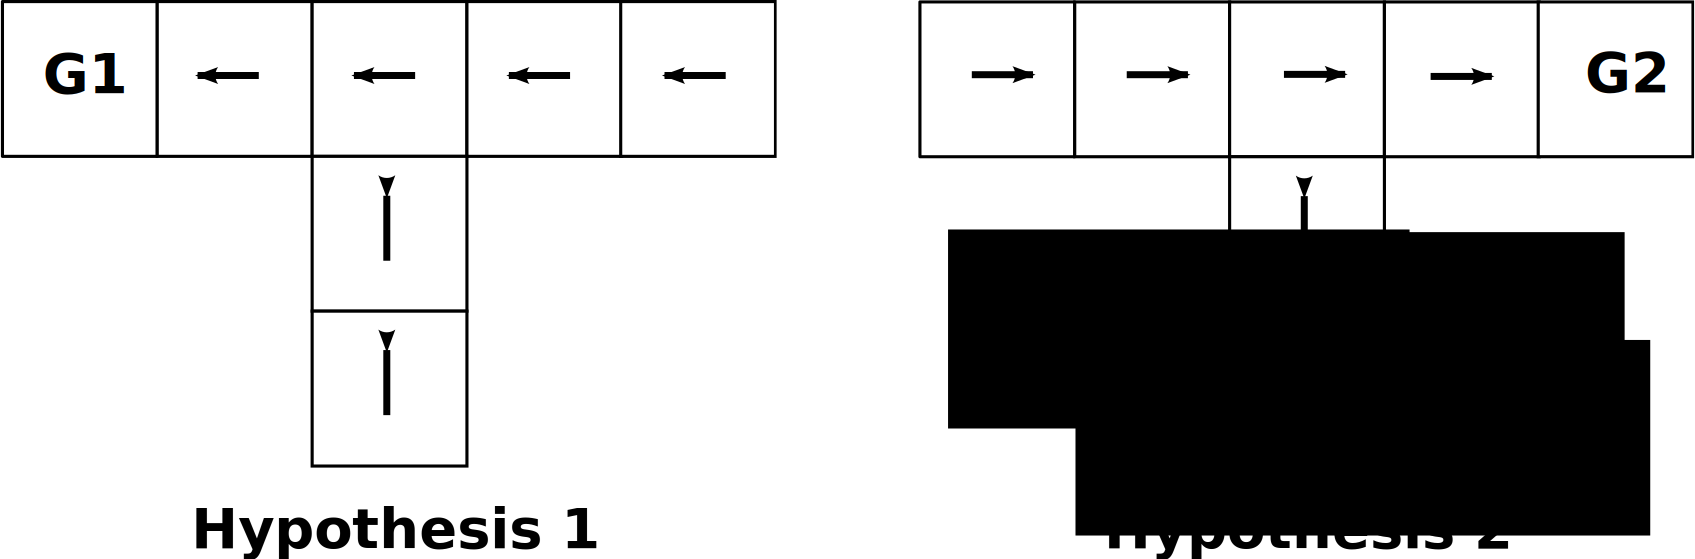
\includegraphics[width=\tworldsize\columnwidth]{\visualspdf/tuto_feedback/Tworld_hypothesis.pdf}
  \caption{Optimal policies associated to the two task hypotheses G1 and G2 in the T world. Such policies are known by both the human and the agent, and allow the agent to interpret a human signal with respect to a given task.}
  \label{fig:Twolrdpolicies}
\end{figure}

The teacher wants the agent to go to G1. The agent starts in state 3, performs action left, and ends-up in state 2. The teacher sends a signal in the right part of the feature space, meaning that the previous action was ``correct''. However the agent does not have access to the label associated to this signal and it only observes a point in a two dimensional space (Figure~\ref{fig:TworldLabelunknown}). The agent generates interpretation hypothesis according to G1 and G2. With respect to G1, the action was ``correct'' (Figure~\ref{fig:TworldLabelG1}), while with respect to G2 the action was ``incorrect'' (Figure~\ref{fig:TworldLabelG1}).

\begin{figure}[!htbp]
    \centering
    \begin{subfigure}[b]{\tworldsize\columnwidth}
        \centering
        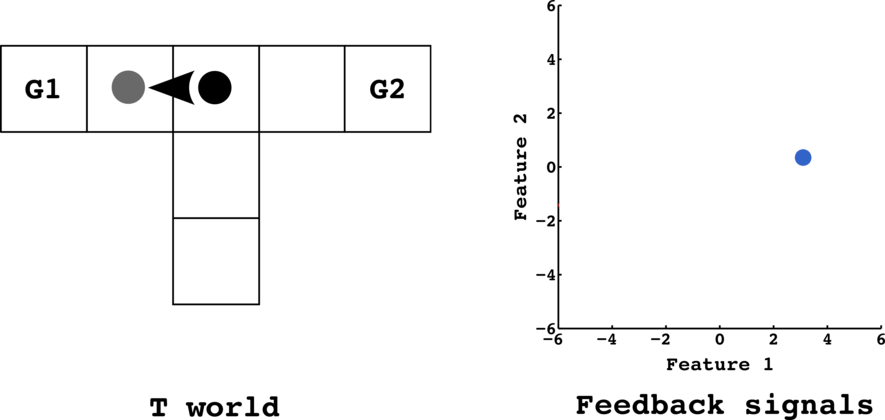
\includegraphics[width=\columnwidth]{\visualspdf/tuto_feedback/Tworld_feedback_unlabeled_one_action.pdf}
        \caption{Feedback signal as received by the agent without label.}
        \label{fig:TworldLabelunknown}
    \end{subfigure}\\
    \begin{subfigure}[b]{\tworldsize\columnwidth}
        \centering
        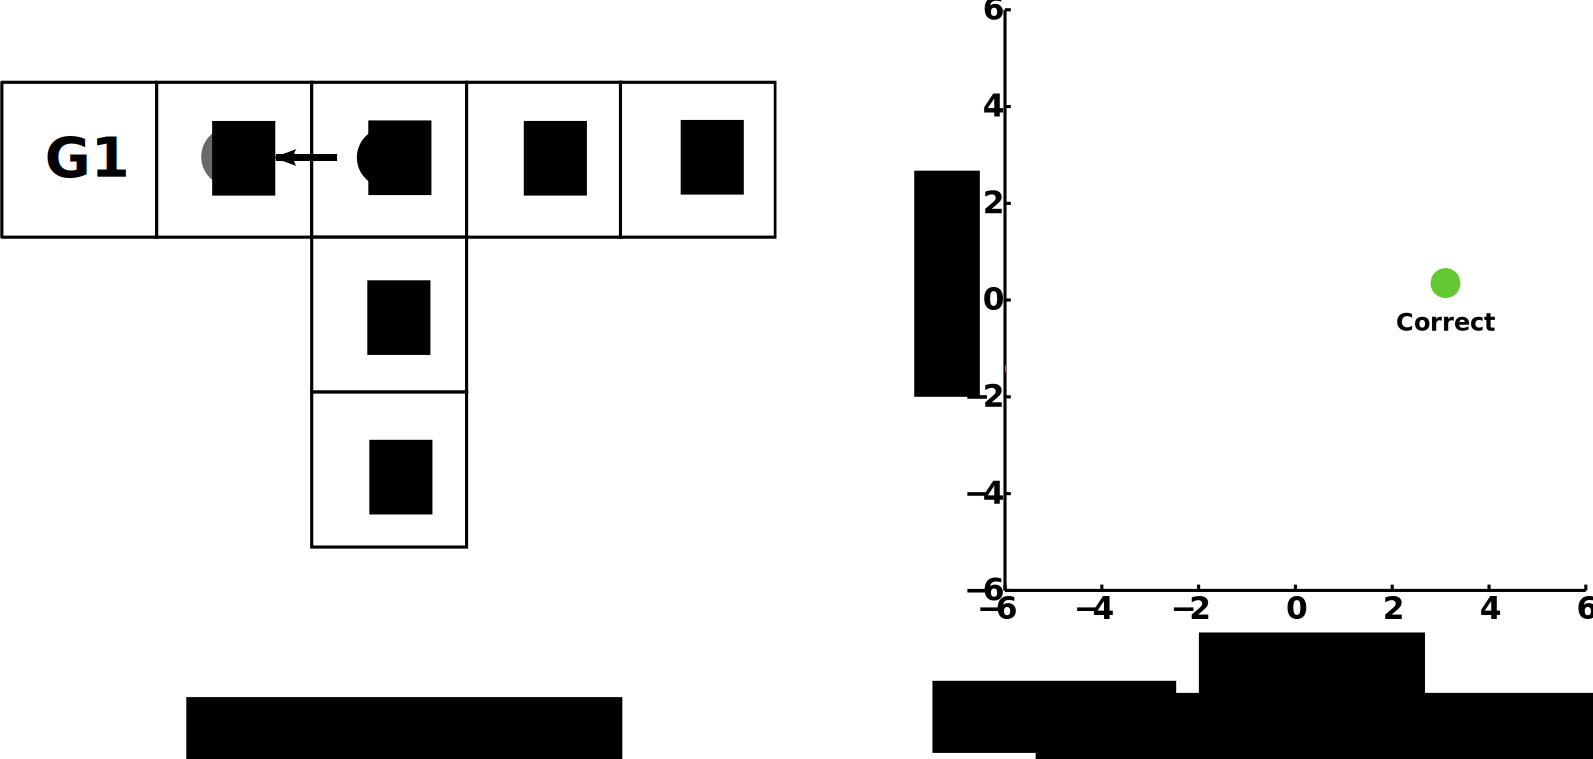
\includegraphics[width=\columnwidth]{\visualspdf/tuto_feedback/Tworld_feedback_labeled_G1.pdf}
        \caption{Feedback signal labeled according to G1.}
        \label{fig:TworldLabelG1}
    \end{subfigure}
    \begin{subfigure}[b]{\tworldsize\columnwidth}
        \centering
        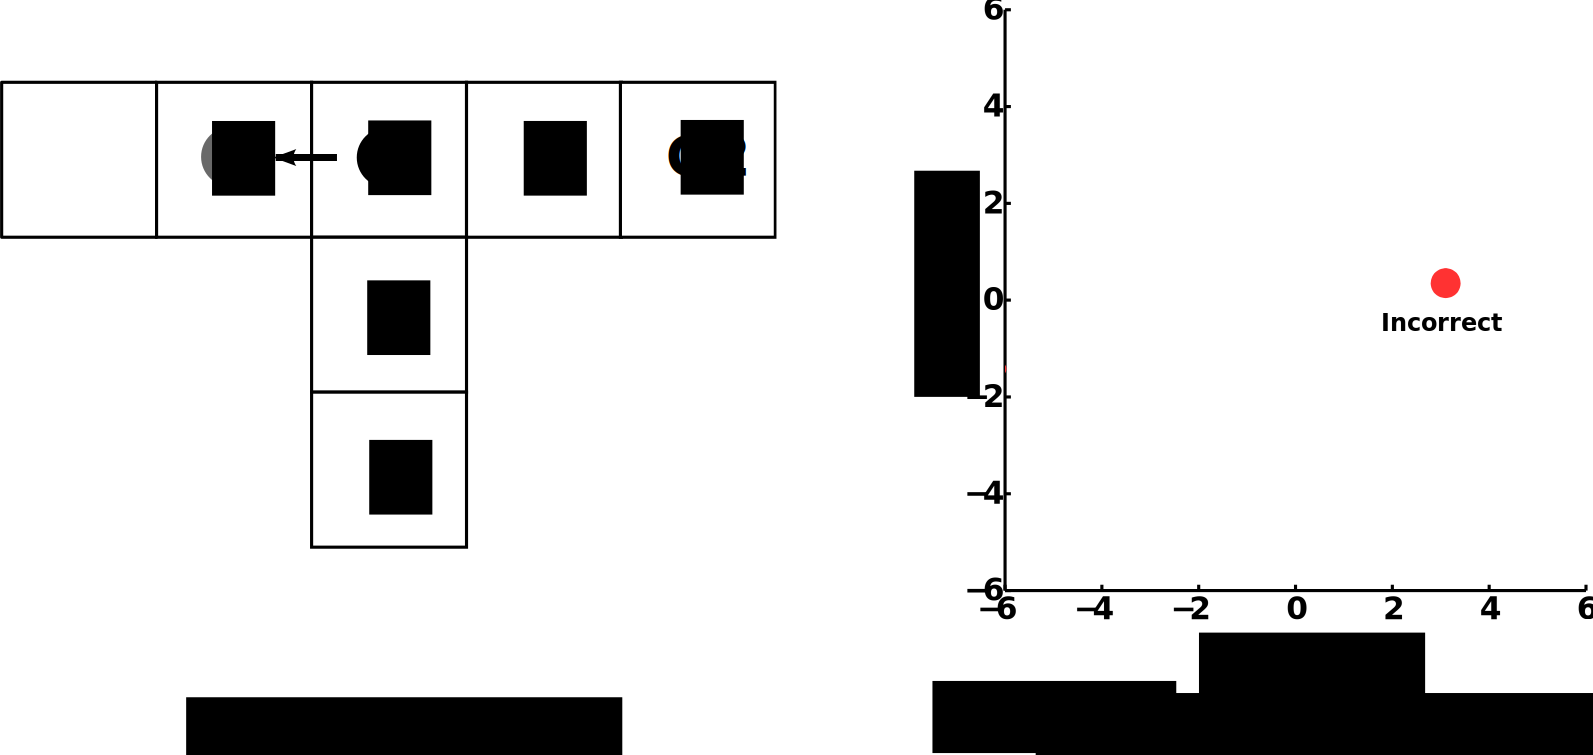
\includegraphics[width=\columnwidth]{\visualspdf/tuto_feedback/Tworld_feedback_labeled_G2.pdf}
        \caption{Feedback signal labeled according to G2.}
        \label{fig:TworldLabelG2}
    \end{subfigure}
    \caption{Interpretation hypothesis made by the agent according to G1 (\ref{fig:TworldLabelG1}) and G2 (\ref{fig:TworldLabelG2}). The agent starts in state 3, performs action left, and ends-up in state 2. The meaning of the signal is different for both hypotheses.}
    \label{fig:TworldLabelOneStep}
\end{figure}

By repeating this process for several iteration steps, with the agent taking random actions, the system end-up with a set of possible interpretation of the human teaching signals (see Figure~\ref{fig:TworldLabelinterpretation}). But as the user has only one objective in mind, in our case G1, only the correct interpretation will assign the correct labels to the observed signals. We say that the corresponding hypothesis exhibit a coherence between the signals and their associated meanings. 

% Note that when the agent moves in the trunk of the T, the interpretation hypothesis with respect to G1 an G2 give the same labels. Details about this interaction will be given in chapter~\ref{chapter:planning} to explain the problem of planning, here we assume the robot explores all state-action.

% \begin{figure}[!htbp]
%     \centering
%     % \begin{subfigure}[t]{\tworldsize\columnwidth}
%     %     \centering
%     %     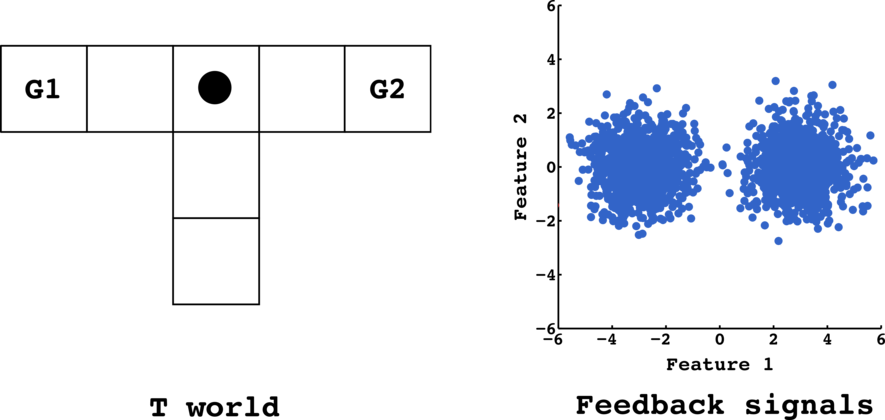
\includegraphics[width=\columnwidth]{\visualspdf/tuto_feedback/Tworld_feedback_unlabeled.pdf}
%     %     \caption{Feedback signals as received by the agent without label.}
%     % \end{subfigure}\\
%     % \begin{subfigure}[b]{\columnwidth}
%         % \centering
%         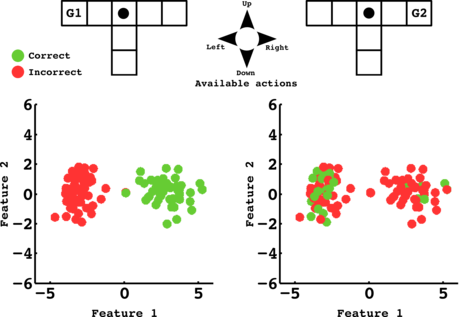
\includegraphics[width=\columnwidth]{\visualspdf/tuto_feedback/Tworld_feedback_labeled_all_actions.pdf}
%         % \caption{Feedback signal labeled according to G1 and G2.}
        
%     % \end{subfigure}
%     \caption{Interpretation hypothesis made by the agent according to G1 and G2 after many interaction steps. The teacher's task is to have the agent reach G1. The agent is exploring all the state space randomly. The labels associated to the task G1 are more coherent with the spacial organization of signals in the feature space.}
%     \label{fig:TworldLabelinterpretation}
%     % \label{fig:TworldLabel}
% \end{figure}

\begin{figure}[!htbp]
    \centering
    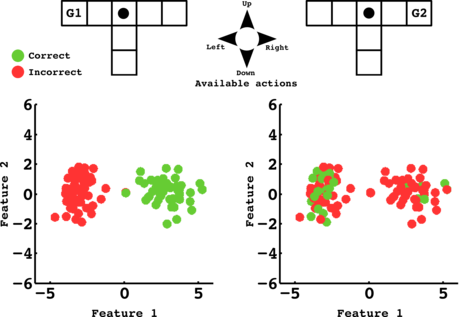
\includegraphics[width=\tworldsize\columnwidth]{\visualspdf/tuto_feedback/Tworld_feedback_labeled_all_actions.pdf}
    \caption{Interpretation hypothesis made by the agent according to G1 and G2 after many interaction steps. The teacher's task is to have the agent reach G1. The agent is exploring all the state space randomly. The labels associated to the task G1 are more coherent with the spacial organization of signals in the feature space.}
    \label{fig:TworldLabelinterpretation}
\end{figure}

Part of the \emph{learning from unlabeled interaction frames} problem defined in chapter~\ref{chapter:introduction:lfui} is the assumption that the user is coherent and uses always the same kind of signal for the same meaning. By visual inspection, we can infer that hypothesis G1 is the correct one as the resulting mapping between signal and meaning is more coherent. The key challenge is to find out how to identify coherence between the spacial organization of signals in the feature space and their associated labels with the tools available to the robot, i.e. algorithmically. 

We will formalize this idea in section~\ref{chapter:lfui:how}. Before that, we add two comments to this section and we summarize all the underlying assumptions of our problem in section~\ref{chapter:lfui:assumptions}.

\subsection{Different frames}

In our example, we considered only the feedback frames, where the user assesses the robot's actions. In this thesis, we will also consider other interaction frame, such as the guidance frame where the user indicates to the robot which action to perform next. We will provide several visual examples of the guidance frame in the following of this chapter.

% , we simply illustrate here the signal that will be associated to the different action. As depicted in Figure~\ref{fig:guidancesignals}, we used an easy to remember way of presenting the data, the cluster at the top of the feature space represents the ``up'' action, the one at the bottom the ``down'' action, the one at the right the ``right'' action, and the one at the left the ``left'' action.

% \begin{figure}[!htbp]
%   \centering
%   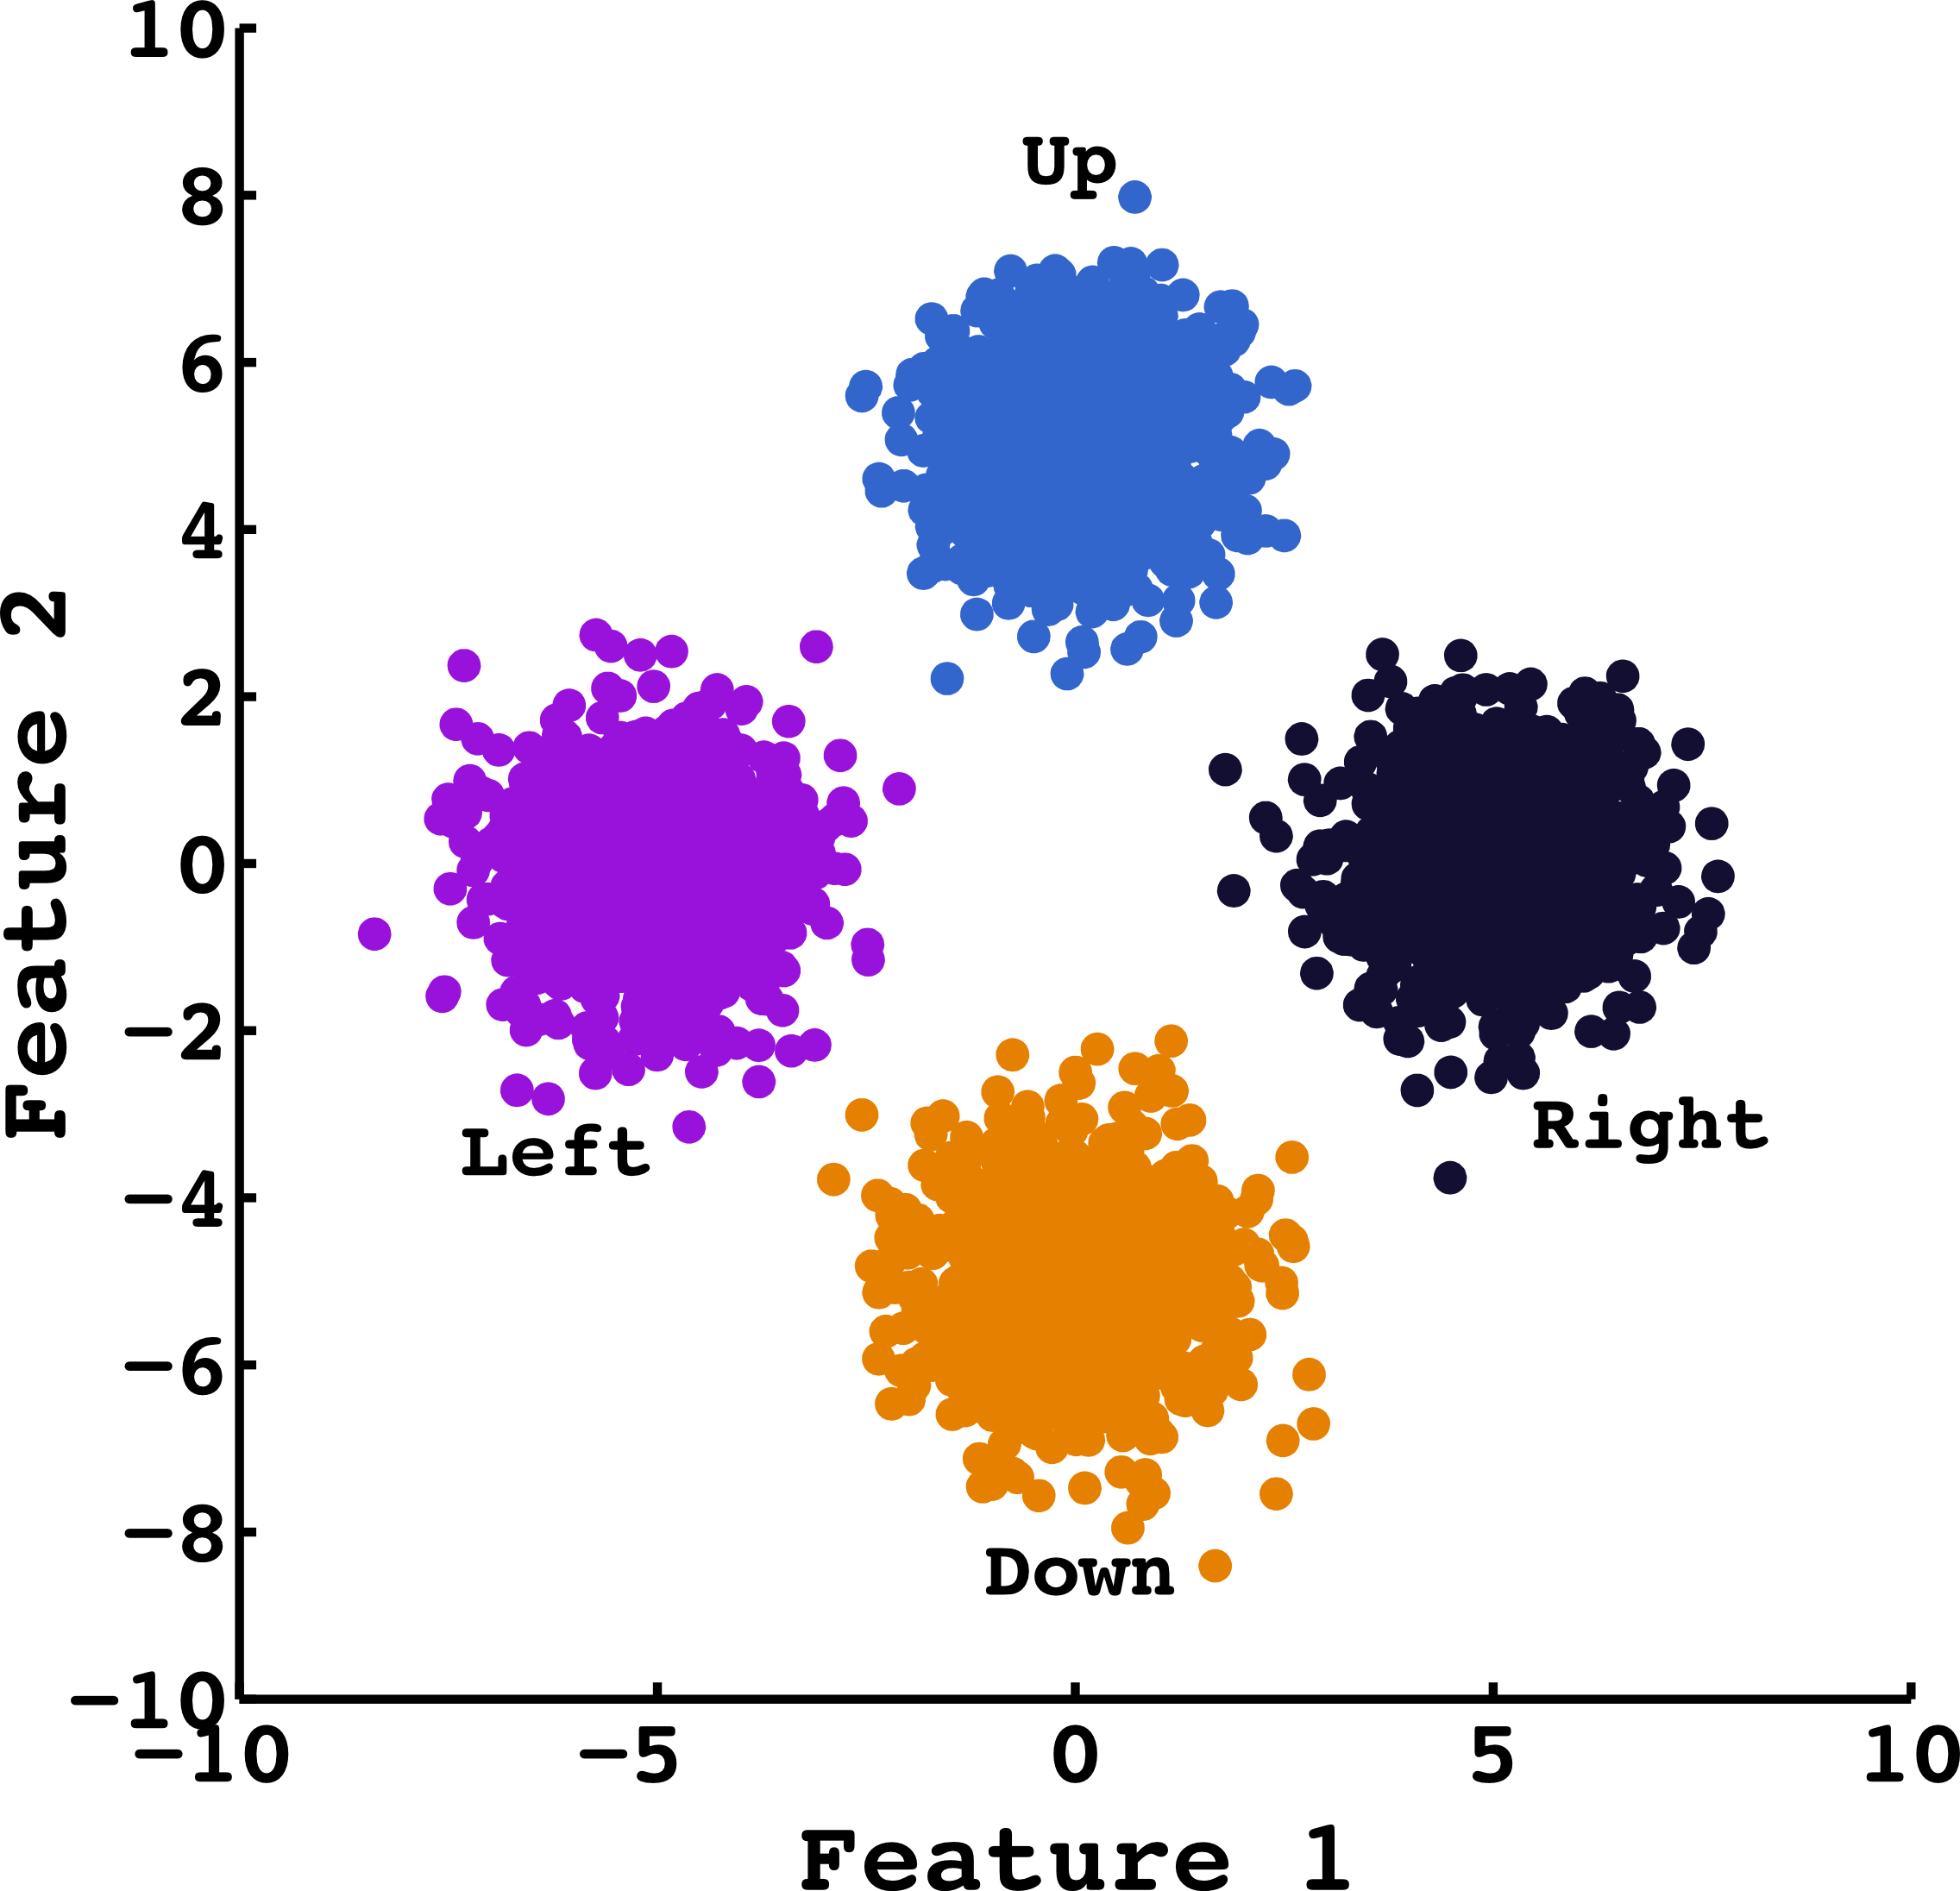
\includegraphics[width=\signalwidth\columnwidth]{\visualspdf/worlds_and_dataset/guidance_4_signals_color.pdf}
%   \caption{The guidance signals used by our simulated teacher in our visual examples.}
%   \label{fig:guidancesignals}
% \end{figure}

\subsection{Why not a clustering algorithm}
\label{chapter:lfui:whynotEM}

When we first look at the unlabeled signals (see Figure~\ref{fig:TworldManyStepUnlabeled}), the first approach that comes to mind is to use a clustering algorithm to identify the two clusters in the feature space. For simple datasets, like the one used in our example, a clustering algorithm will find the two clusters. However, without any additional information, it is impossible to know which one is associated to the meaning ``correct'' or to the meaning ``incorrect''.

More importantly, clustering algorithms are prone to local extrema in the optimization process and for datasets in high dimension with overlapping classes it is unlikely to find the correct underlying structure of the data. Our approach has the advantage to generate hypothetic labels allowing fitting a classifier for each task hypothesis. 

% several empirical results showed that indeed this is the case for data consisting of speech utterances and brain signals.

%%%%%%%%%%%%%%%%%%%%%%%%%%%%%%%%%%%%%%%%%%%%%%
%%%%%%%%%%%%%%%%%%%%%%%%%%%%%%%%%%%%%%%%%%%%%%
%%%%%%%%%%%%%%%%%%%%%%%%%%%%%%%%%%%%%%%%%%%%%%
%%%%%%%%%%%%%%%%%%%%%%%%%%%%%%%%%%%%%%%%%%%%%%
%%%%%%%%%%%%%%%%%%%%%%%%%%%%%%%%%%%%%%%%%%%%%%
\section{Assumptions}
\label{chapter:lfui:assumptions}

As described in the introduction, a number of assumptions are made about the information accessible to the robot and the constraints applied to the interaction. We remind them again briefly here and, now that we have exemplified the mechanism of interpretation hypotheses, we present an additional required property that the world must hold for our problem to be solvable. We will see that, in some cases, it is impossible to discriminate between two hypotheses because they result in symmetric interpretations of the signals. We describe this properties in subsection~\ref{chapter:lfui:symmetries}.

\subsection{Frames}

Our first assumption is that the robot and the human are aware of the frame in which the interaction takes place. This frame regulates the interaction between the two partners, it includes:

\begin{itemize}

\item \textbf{Details and timing of the interaction.} It corresponds to when and how the user will provide instruction signals. For example, the human sends a signal to the robot after every robot's actions. Another example is a human providing a feedback signal between 0.2 and 2 seconds after the robot's action \cite{knox2009interactively}.

\item \textbf{The set of possible meanings the human can refer to.} As depicted before, the set of meaning may include ``correct'' and ``incorrect'' for those cases where the user is assessing the robot's actions. It could also be the set of action names when the user provides guidances on what to do next.

\item \textbf{Constraints on the possible tasks.} The general context of the teaching process is known. For example the robot is aware that the human wants it to reach a specific room in the house, and not to take an object from the fridge. This limits the number of hypotheses the robot can create about what the user has in mind.

\end{itemize}

By combining those three aspects of an interaction frame, the robot can create a set of interpretation hypothesis for the received teaching signals. For one possible task, and given a specific context (e.g. state and action performed in the environment), the robot can infer the meaning intended by the human user ($Meaning = Frame(Context, Task)$). By doing so for every possible task, the agent creates a set of interpretation hypothesis, which we rely on to find the task taught by the user, as well as the signal to meaning mapping.

To do so we rely on specific properties of the human teaching signals.

\subsection{Signals properties}
\label{chapter:lfui:signalproperties}

We make two assumptions about the human teaching signals properties:

\begin{itemize}

\item If the true intended meaning associated to each user signal was known, it would be possible to train a classifier with better than random accuracy. We will see in chapter~\ref{chapter:planning:results} that the performance of the system are highly impacted by the quality of the training data.

\item The teacher is consistent in its use of teaching signals and will always use the name kind of signals to mean the same things. For the case of two buttons, he will always use the same button for the same meaning. It also applies for speech, facial expression, gestures, or brain signals. 

\end{itemize}

Those two properties are typical assumptions in human-robot interaction scenario, we simply assume we can rely on the teacher behavior and that we could, in theory, learn a decoder of the human teaching signals.

However there is one practical constraint that differs from more standard human-robot interaction scenario. Here, in theory, we cannot know in advance if a signal to meaning mapping can be learn. Indeed we do not have access to a database of signal-meaning pairs to train a classifier first, which allow trying different feature extraction processes or different classifiers beforehand. This limitation requires ensuring the representation of the signal and the classifier allow to learn a usable decoder.

We will see from results in chapter~\ref{chapter:planning:results} that our algorithm can cope with highly overlapping data where the classifier produces close to random prediction.

\subsection{World properties and symmetries}
\label{chapter:lfui:symmetries}

There are some cases where different hypothesis are not distinguishable. As the robot do not have a direct access to the true intended meaning of the teaching signals, it can only rely on the interpretation hypothesis made for each task.

Two problems could appear: \begin{inparaenum}[(a)] \item two hypothesis may share the same interpretation model and cannot be differentiated as they attribute the same meanings to the signals, and \item two hypothesis may end up with opposite interpretations that are both as valid. \end{inparaenum}.

For those cases where two hypothesis share the same interpretation model, either the task are the same with respect the user, either some parts of the problem are hidden to the human, which can not provide appropriate instructions. These questions are the core of the theoretical analysis of Cederborg's thesis \cite{cederborg2014thesis,cederborg2014social}. We do not consider this problematic in this thesis and assume the world properties ensure that two hypothesis will never share the same interpretation model. Most of the hypothesis will share parts of the interpretation model but it will always exist one situation, i.e. one state-action pair, where two interpretation models differs.

For those cases where two hypotheses end up with opposite interpretations that are both valid, we illustrate the problem for the case of both feedback and guidance instructions using a visual example.

\subsubsection*{Symmetries: the feedback case}

We present the line word in Figure~\ref{fig:lineworld} which contains only the top T bar of the T world. This world is well suited to describe the symmetry problem. 

\begin{figure}[!htbp]
  \centering
  
\includegraphics[width=\tworldsize\columnwidth]{\visualspdf/worlds_and_datasets/lineworld_with_state_number_and_2action.pdf}
  \caption{The line world and the available actions.}
  \label{fig:lineworld}
\end{figure}

The interaction follows the same protocol as in previous examples. As depicted in Figure~\ref{fig:lineworldfeedback2action}, after several interaction steps, the interpretation hypothesis for G1 and G2 display symmetric properties. Indeed, according to G1, signals on the left side of the feature space mean ``incorrect'', and signal on the right means ``correct''. Inversely, according G2, signals on the left side of the feature space mean ``correct'', and signal on the right means ``incorrect''. Therefore, even if the interpretation of the signals differs between each hypothesis, the two interpretations are equally coherent. As the optimal policies to reach each of the two goal states are opposite in every state, an action that triggers a ``correct'' feedback with respect to G1, triggers a ``incorrect'' feedback for G2 and vice versa. It is therefore impossible to know the true associated meaning of the signals without further information.

\begin{figure}[!htbp]
  \centering
  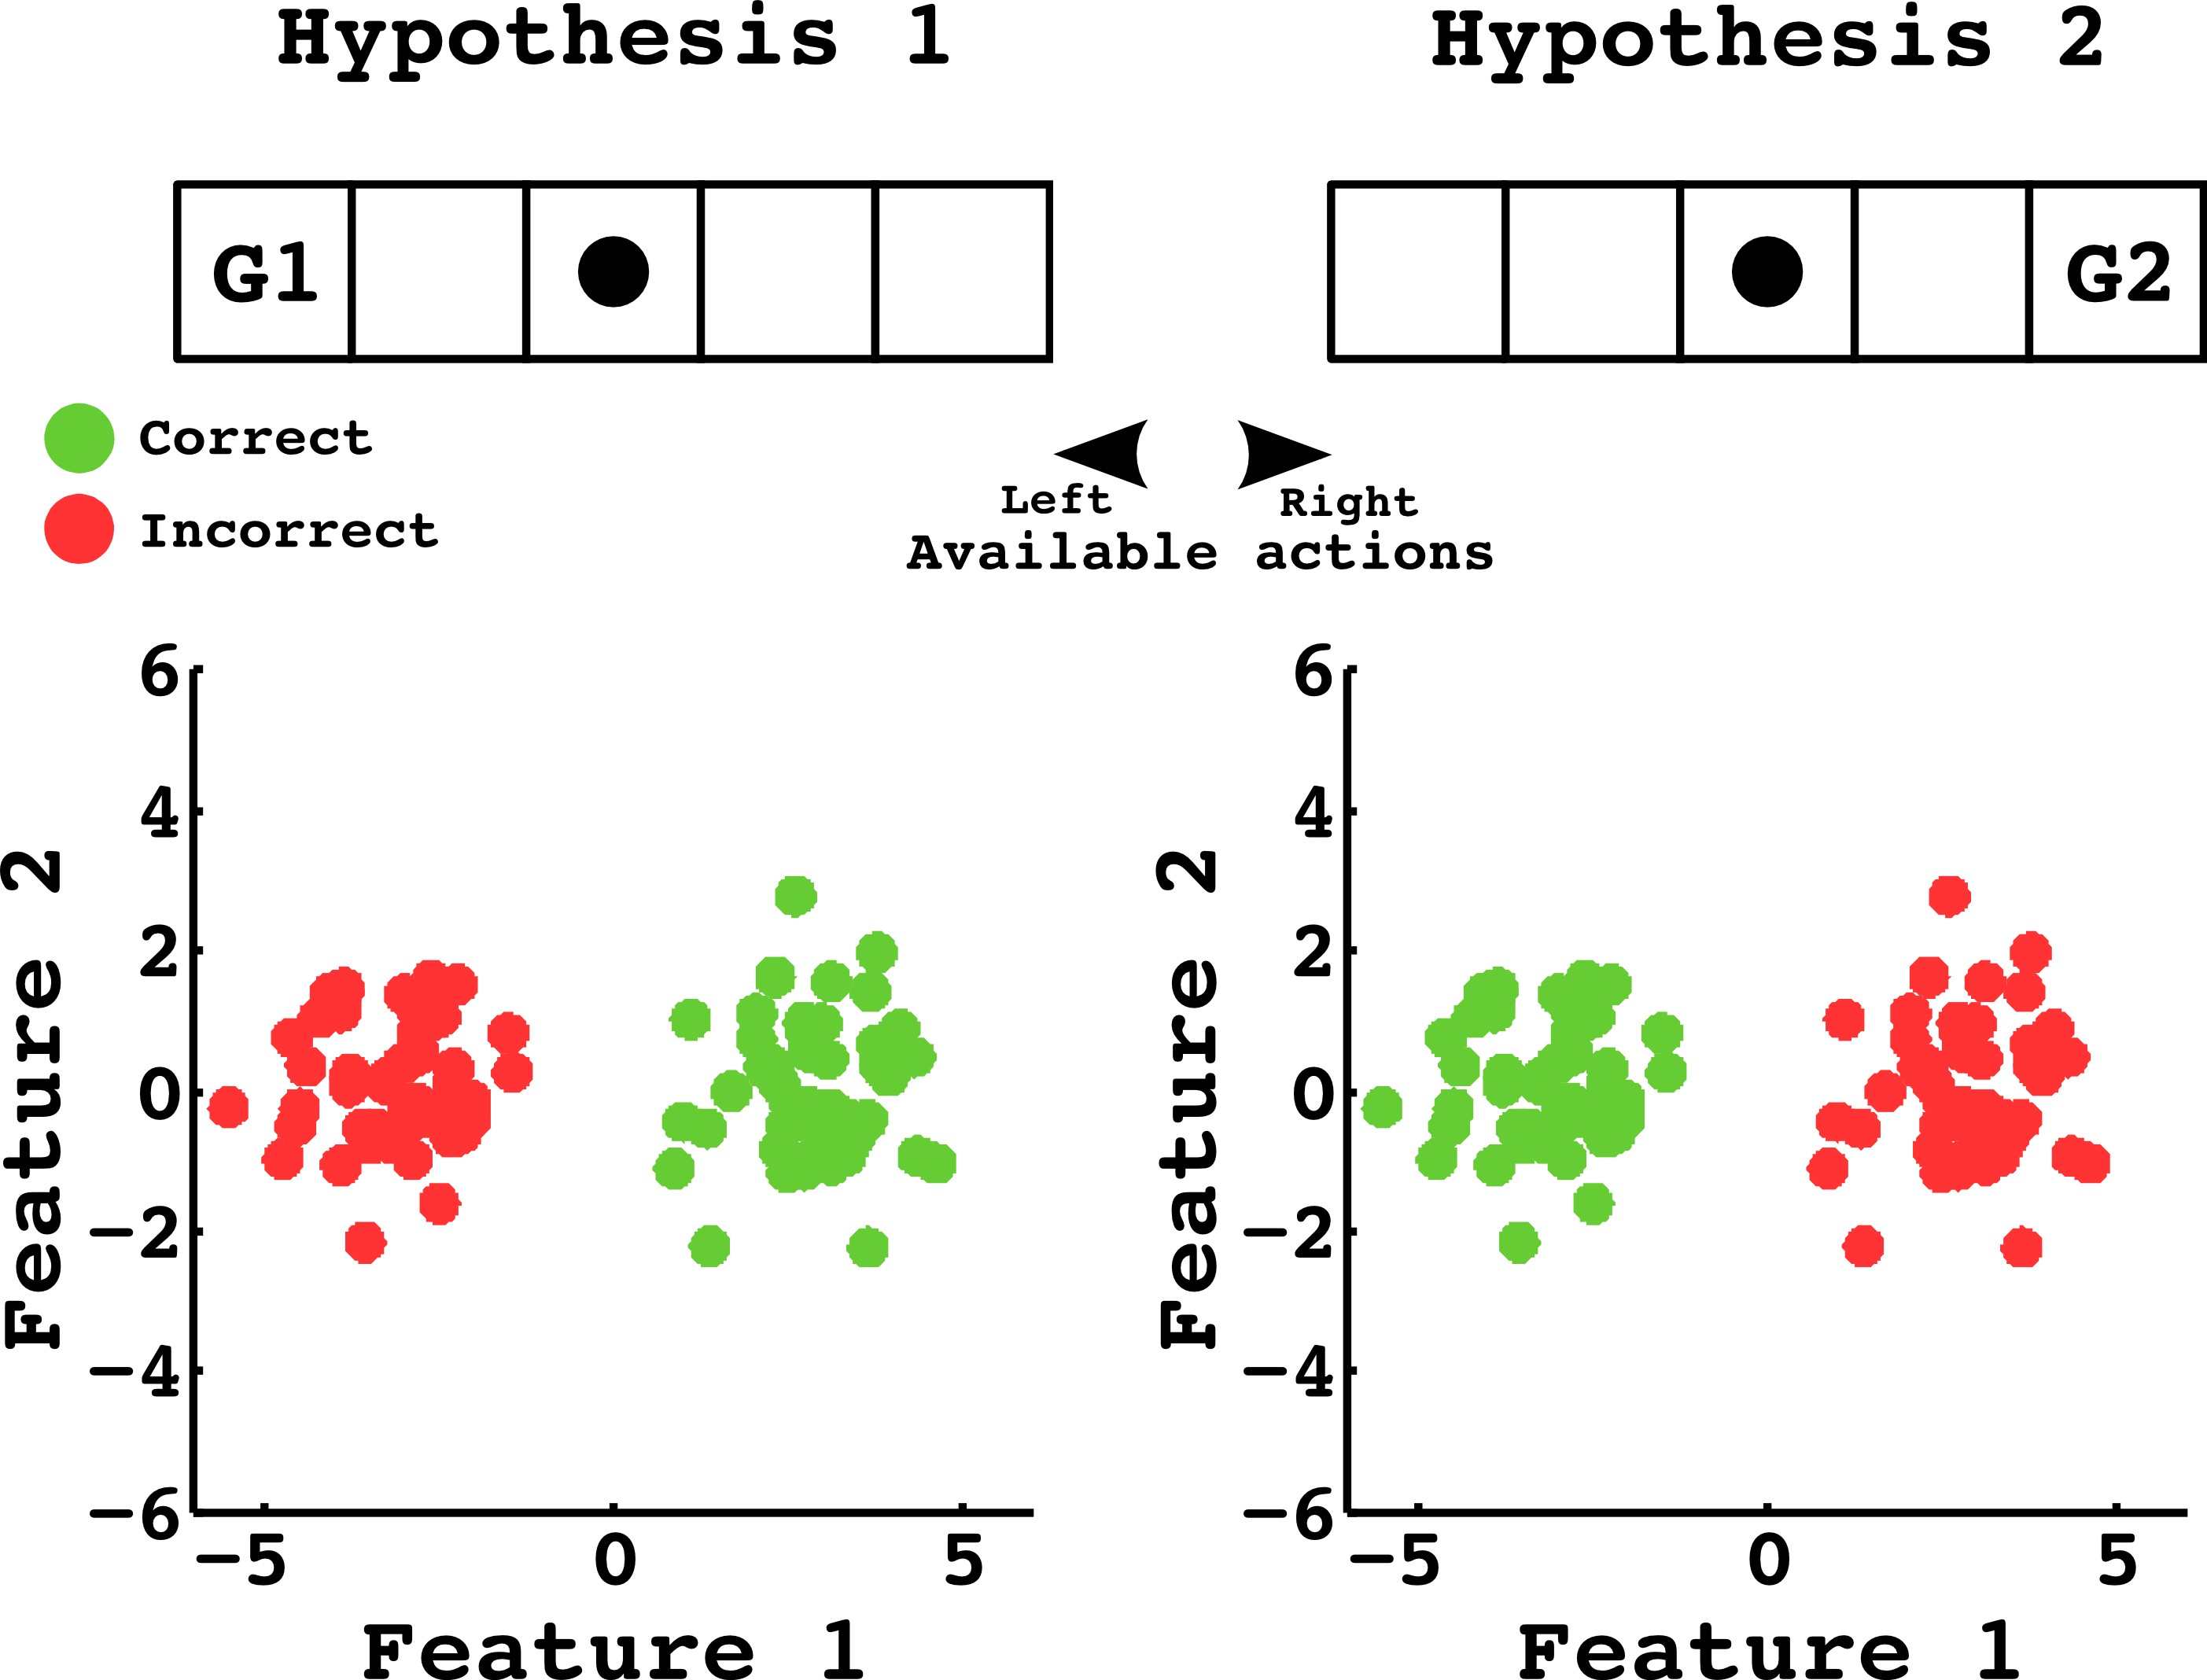
\includegraphics[width=\tworldsize\columnwidth]{\visualspdf/lineworld_symmetries/feedback_2actions.pdf}
  \caption{Interpretation hypotheses made by an agent receiving feedback on its action in the line word and where the hypothetic tasks are G1 or G2. The agent can only perform right or left actions which results in symmetric interpretation hypothesis of the feedback signals.}
  \label{fig:lineworldfeedback2action}
\end{figure}

It is theoretically impossible to differentiate symmetric task hypotheses, therefore we will not consider environments holding this symmetric property. One way to bypass this problem is to add a ``no move'' action, as illustrated in Figure~\ref{fig:lineworld3action}, that is valid only at the goal state

\begin{figure}[!htbp]
  \centering
  
\includegraphics[width=\tworldsize\columnwidth]{\visualspdf/worlds_and_datasets/lineworld_with_state_number_and_action.pdf}
  \caption{The line world and the new available actions, including a ``no move'' action.}
  \label{fig:lineworld3action}
\end{figure}

When taking the ``no move'' action the agent does not change position. This action allow to brake the symmetry effects, as its interpretation will be the same for all states that are not in the set of hypothetic goal state, i.e. all state but G1 and G2. In other words, if the agent performs action ``no move'' in state 3, the user will produce a signal of meaning ``incorrect'' because the agent is not progressing towards the goal state(G1 here). But the agent did not progress either towards the G2. Therefore the signal will be interpreted as ``incorrect'' by the two interpretation hypothesis, breaking the symmetry problem. The interpretation results after several iteration steps, and using the new ``no move'' action, are depicted in Figure~\ref{fig:lineworldfeedback3action}.

\begin{figure}[!htbp]
  \centering
  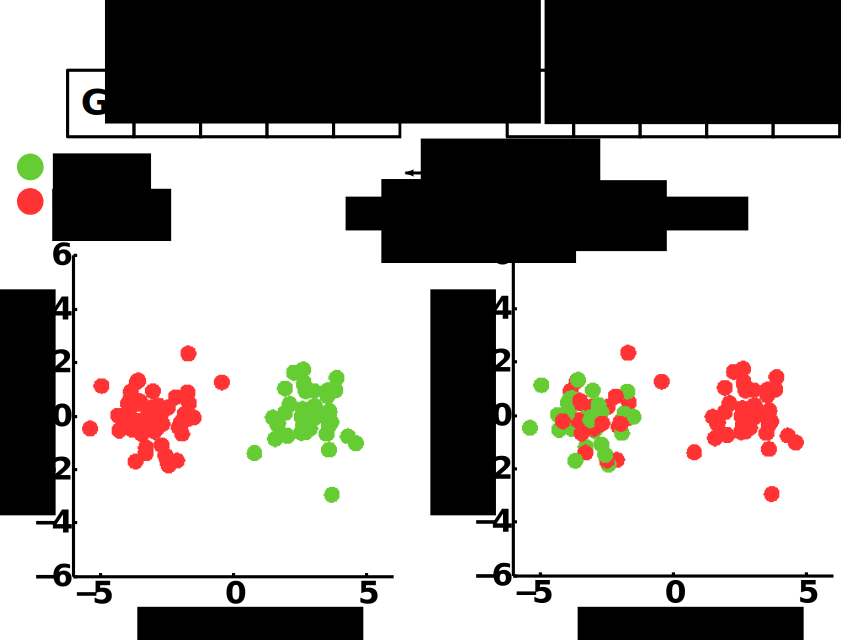
\includegraphics[width=\tworldsize\columnwidth]{\visualspdf/lineworld_symmetries/feedback_3actions.pdf}
  \caption{Interpretation hypotheses made by an agent receiving feedback on its action in the line word and where the hypothetic tasks are G1 or G2. The agent can perform right, left, or ``no move'' actions. As opposed to Figure~\ref{fig:lineworldfeedback2action}, the ``no move'' action allows to break the symmetry of interpretation between G1 and G2.}
  \label{fig:lineworldfeedback3action}
\end{figure}

\subsubsection*{Symmetries: the guidance case}

This problem of symmetries also applies to the guidance frame. Under the guidance frame, the set of possible meaning includes the name of all possible actions. If the agent can only choose between the ``right'' and ``left'' actions, the teacher can only advise for ``left'' and ``right'' actions. We represent the guidance signals from the teacher in a two dimensional feature space as shown in Figure~\ref{fig:lineworldguidance2signals}.

\begin{figure}[!htbp]
  \centering
  \includegraphics[width=\signalwidth\columnwidth]{\visualspdf/worlds_and_datasets/guidance_2_signals_color.pdf}
  \caption{The guidance signals used by our simulated teacher in our line world visual examples with two actions.}
  \label{fig:lineworldguidance2signals}
\end{figure}


We can easily understand that if the teacher can only advise for ``left'' and ``right'' actions, the interpretation hypothesis for G1 will be symmetric as the one for G2. As our user wants the robot to reach G1, it will only produce ``left'' guidance signals, i.e. signals in the left part of the feature space. And the ``right'' commands will never be used. However, these signals will be interpreted as meaning ``left'' according to G1, and ``right'' according to G2. Yet the two interpretation models are equally coherent. The resulting interpretation hypothesis are shown in Figure~\ref{fig:lineworldguidance2action}.

\begin{figure}[!htbp]
  \centering
  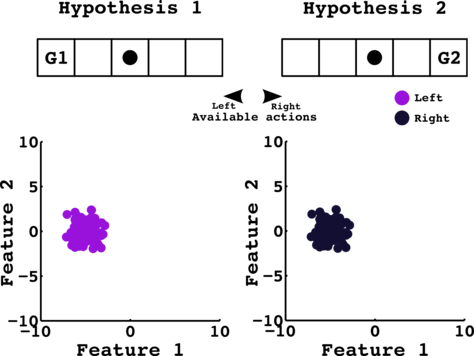
\includegraphics[width=\tworldsize\columnwidth]{\visualspdf/lineworld_symmetries/guidance_2actions.pdf}
  \caption{Interpretation hypotheses made by an agent receiving guidance on its actions in the line word and where the hypothetic tasks are G1 or G2. The agent can only perform right or left actions which results in symmetric interpretation hypothesis of the guidance signals.}
  \label{fig:lineworldguidance2action}
\end{figure}

As for the feedback case, introducing a ``no move action'' allow to break the symmetry. With the ``no move'' action available, the user can now produce three different kinds of meaning, which is represented by three different clusters of signals in the feature space (see Figure~\ref{fig:lineworldguidance3signals}). 

\begin{figure}[!htbp]
  \centering
  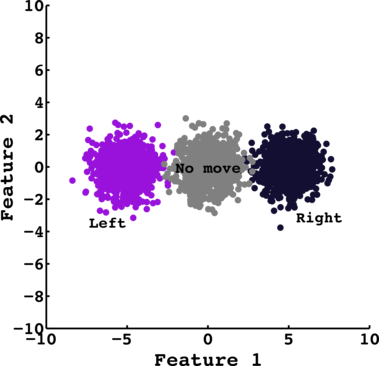
\includegraphics[width=\signalwidth\columnwidth]{\visualspdf/worlds_and_datasets/guidance_3_signals_color.pdf}
  \caption{The guidance signals used by our simulated teacher in our line world visual examples with three actions.}
  \label{fig:lineworldguidance3signals}
\end{figure}

The ``no move'' signal will be used only at the goal state. As this state is not the same for each hypothesis, the ``no move'' signals break the symmetry. The resulting interpretation hypothesis are shown in Figure~\ref{fig:lineworldguidance3action}.

\begin{figure}[!htbp]
  \centering
  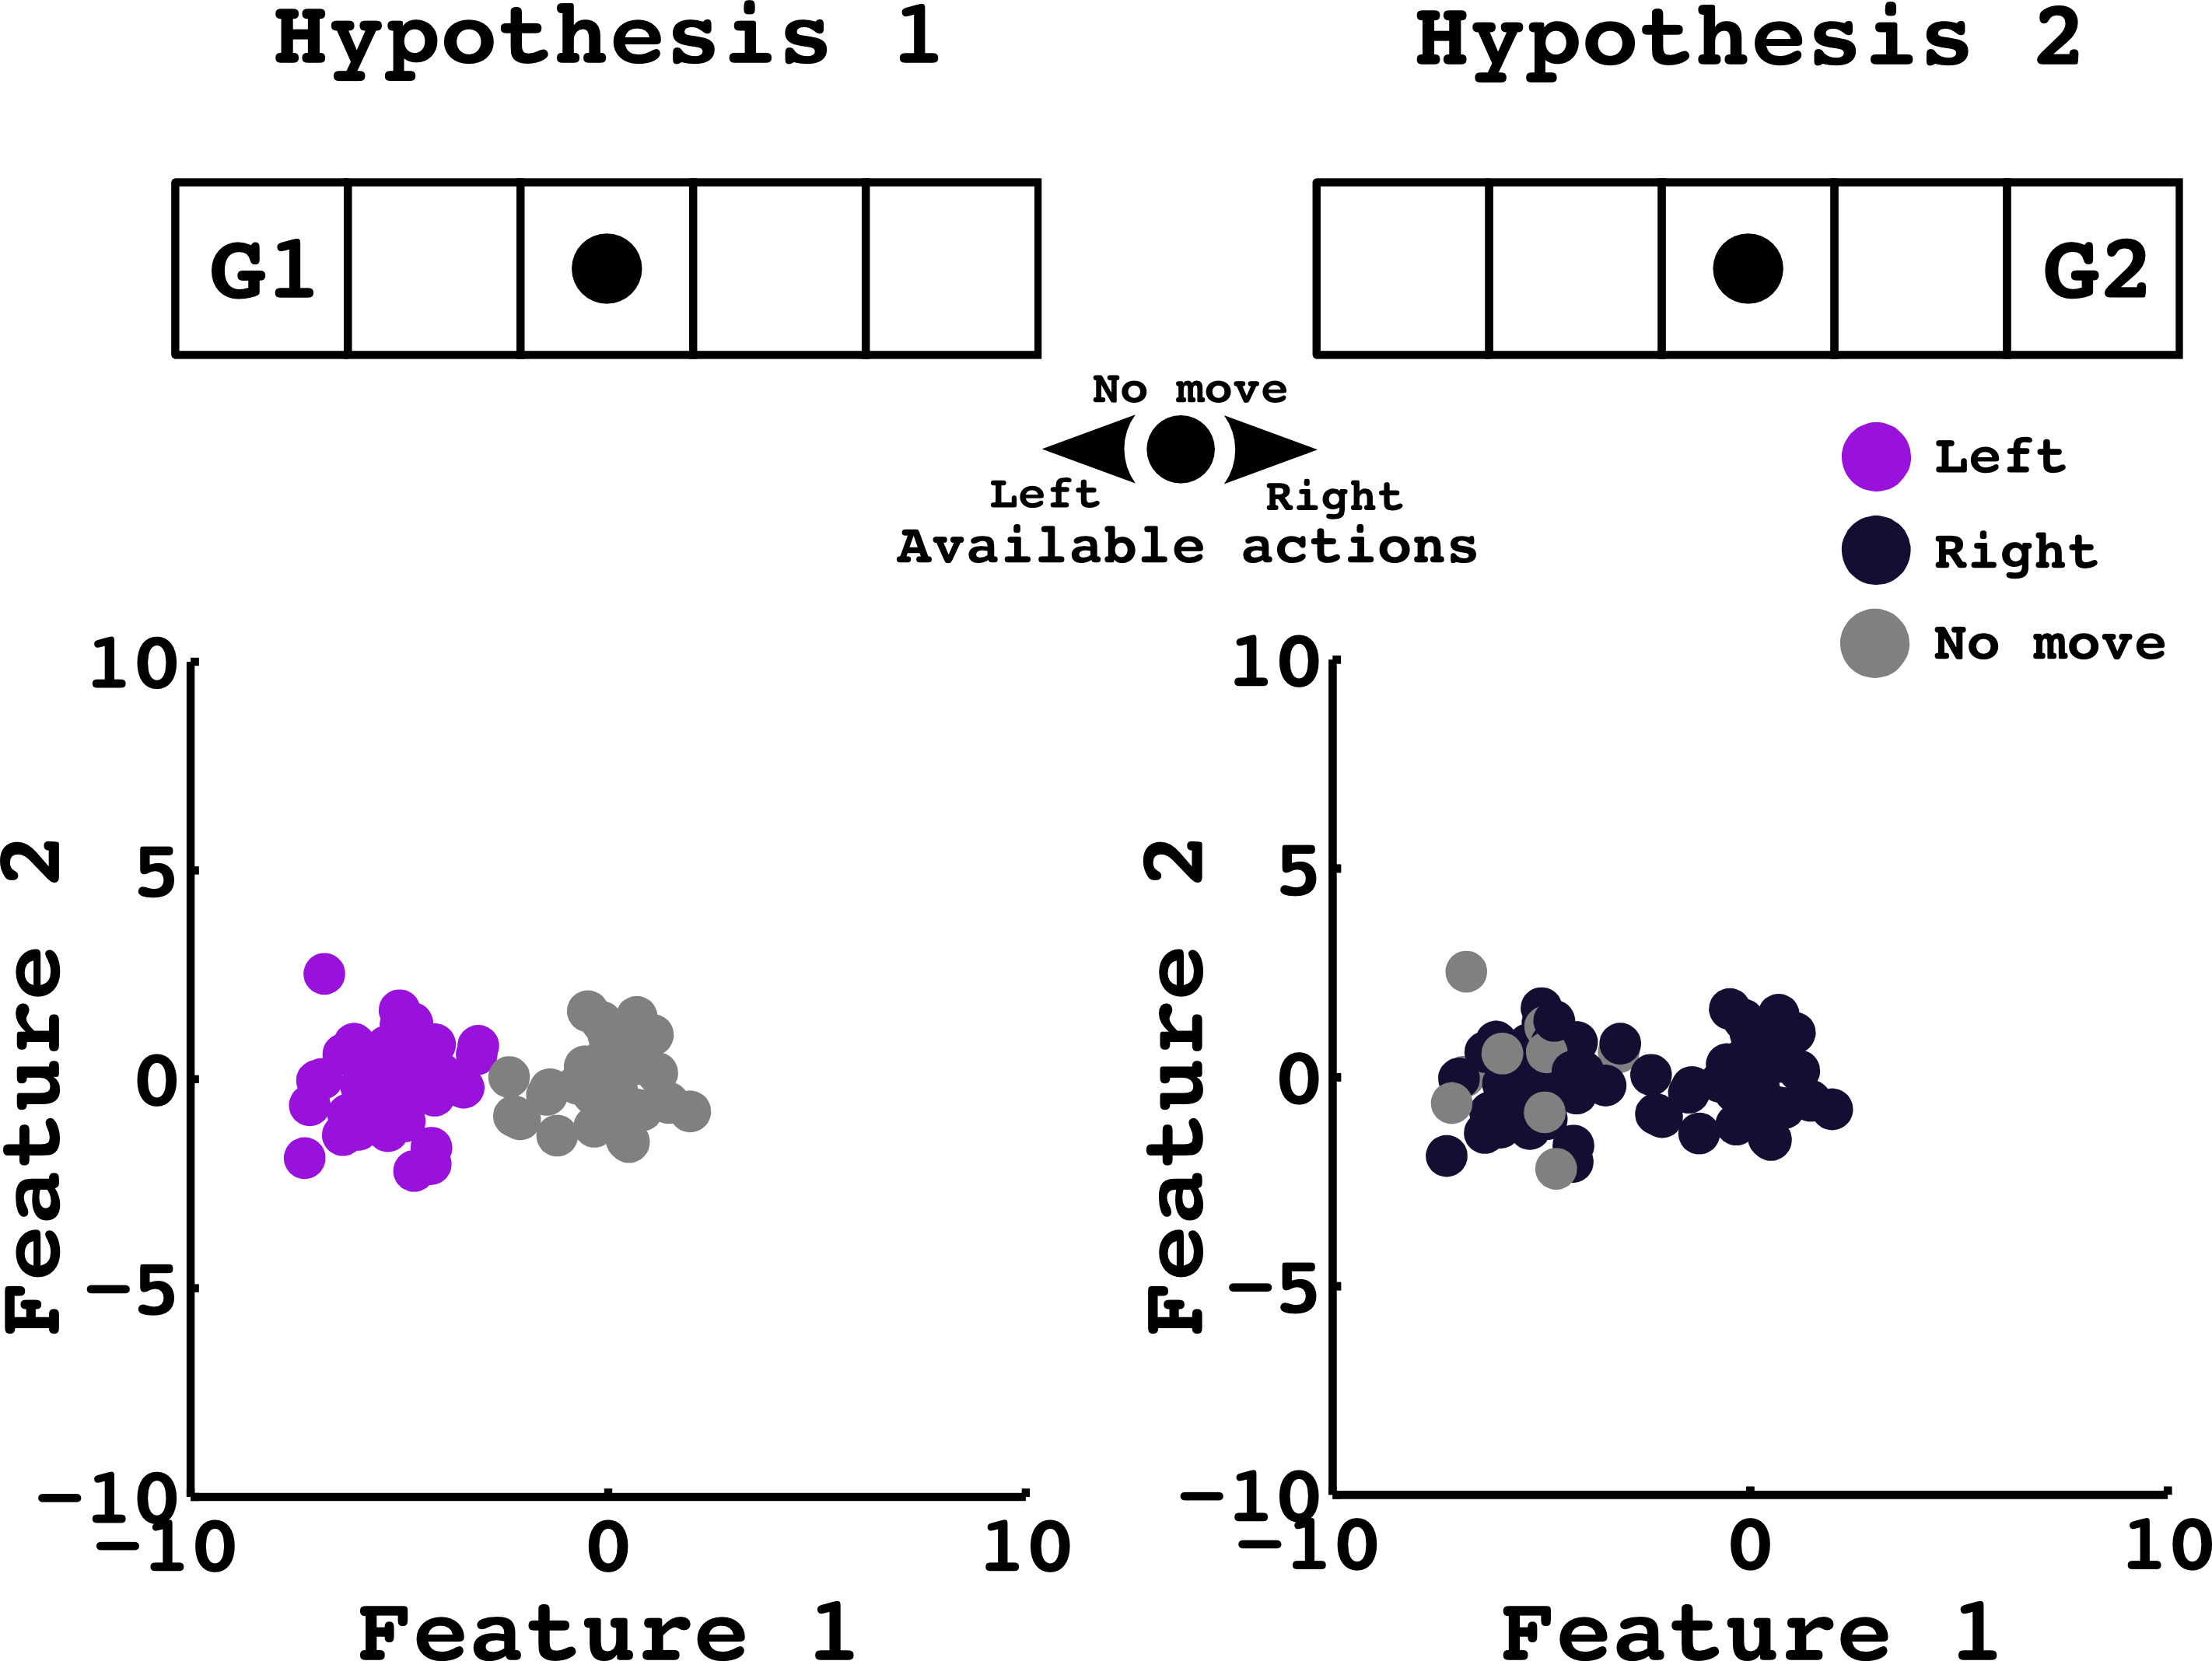
\includegraphics[width=\tworldsize\columnwidth]{\visualspdf/lineworld_symmetries/guidance_3actions.pdf}
  \caption{Interpretation hypotheses made by an agent receiving guidance on its actions in the line word and where the hypothetic tasks are G1 or G2. The agent can perform right, left, or ``no move'' actions. As opposed to Figure~\ref{fig:lineworldguidance2action}, the ``no move'' action allows to break the symmetry of interpretation between G1 and G2.}
  \label{fig:lineworldguidance3action}
\end{figure}

\transition

As it is theoretically impossible to differentiate symmetric task hypotheses, we will not consider environments holding this symmetric property.

\subsection{Robot's abilities}

We further assume the robot is able to plan its action in order to fulfill a specific task. In other words, if the robot knew what the user wants it to do, it will be able to do it. It implies the robot as full knowledge of the world dynamics and knows how to make a plan. This way the robot can understand the theoretical relation between one action, a specific task and a signal of the user; and therefore create interpretation hypothesis.

% However, this ability could have been learn from previous self-exploration session of the environment allowing the robot to learn the dynamics of the environment.

\transition

The following of this chapter will consider the full set of assumptions defined above.

Most of these constraints are typical from interactive learning experiments. Several aspects are often more constrained. Especially, either the signal to meaning mapping is known in advance, and the agent infer the task based on the known instructions \cite{kaplan2002robotic,chernova09jair,knox2009interactively}, either the task itself is known, allowing the robot to assign meanings to the teaching signals such that the signal to meaning mapping can be learned (e.g. the calibration phase for BCI systems). Our method generalizes over these approaches as we neither need to know the task, nor the signal-to-meaning mapping.

Other constraints are not always applied, such as the ability of the robot to plan its action, or the fact that a finite number of tasks are defined in advance.

The ability to plan is linked to the need for the robot to interpret the signals of the user in different situations. To do so the robot needs to be able to project itself in the future to judge of the ``long term'' effects of its actions. 

% It may be possible to considered an agent that is not able to plan its actions. In such cases, the robot should learn first by self-exploration the dynamic of the environment and  infer a plan for a given task.

The finite set of task hypothesis is more of a practical constraint. Considering an infinite set of task hypothesis would add another layer of complexity. Given our interpretation hypothesis mechanism, we would have to sample a finite number of hypotheses. Then given the results of our hypothesis based method on this finite set, we would have to re-sample some new hypothesis and test them again until some stopping criterion. This sampling process is logically less reliable than assuming the correct task belongs to a finite set. Therefore, in our main experiments, we only consider problems where a finite set of task hypothesis can be defined. It is only in chapter~\ref{chapter:limitations:continuoushypothesis} that this assumption is removed.

%%%%%%%%%%%%%%%%%%%%%%%%%%%%%%%%%%%%%%%%%%%%%%
%%%%%%%%%%%%%%%%%%%%%%%%%%%%%%%%%%%%%%%%%%%%%%
%%%%%%%%%%%%%%%%%%%%%%%%%%%%%%%%%%%%%%%%%%%%%%
%%%%%%%%%%%%%%%%%%%%%%%%%%%%%%%%%%%%%%%%%%%%%%
%%%%%%%%%%%%%%%%%%%%%%%%%%%%%%%%%%%%%%%%%%%%%%
\section{How do we exploit interpretation hypotheses}
\label{chapter:lfui:how}

As exemplified in Figure~\ref{fig:TworldLabelinterpretation}, generating interpretation hypothesis for each possible task allows to find out the task the user has in mind. As the user has only one objective in mind, only the correct hypothesis will assign the correct meanings to the observed signals. In our example, we can identify this task visually, by looking at the coherence between the spacial organization of the signals and their associated meanings. But our robots and algorithms cannot use our visual intuition. The key challenge it to find out a measure that can reflect the coherence between the spacial organization of the signals and their associated meanings.

As a measure of coherence we can measure the quality, i.e. the accuracy, of a decoder trained on each hypothetic dataset of signal-label pairs. As for the wrong hypotheses some signals are not associated with their correct meanings, the quality of the resulting classifiers should be worst than the quality of the classifier trained on the correct hypothesis.

For example, if we assume the signals generated by the teacher can be separated by a quadratic curve, and following our T world example (cf. Figure~\ref{fig:TworldLabelinterpretation}), for each task, we can use the quadratic discriminant analysis (QDA) \cite{lachenbruch1975discriminant} approach to fit a classifier on the data. For two classes, this classifier resumes in computing the maximum likelihood for the mean and covariance matrix associated to each labels. The results of this process is illustrated in Figure~\ref{fig:TworldLabelGaussian}.

\begin{figure}[!htbp]
    \centering
    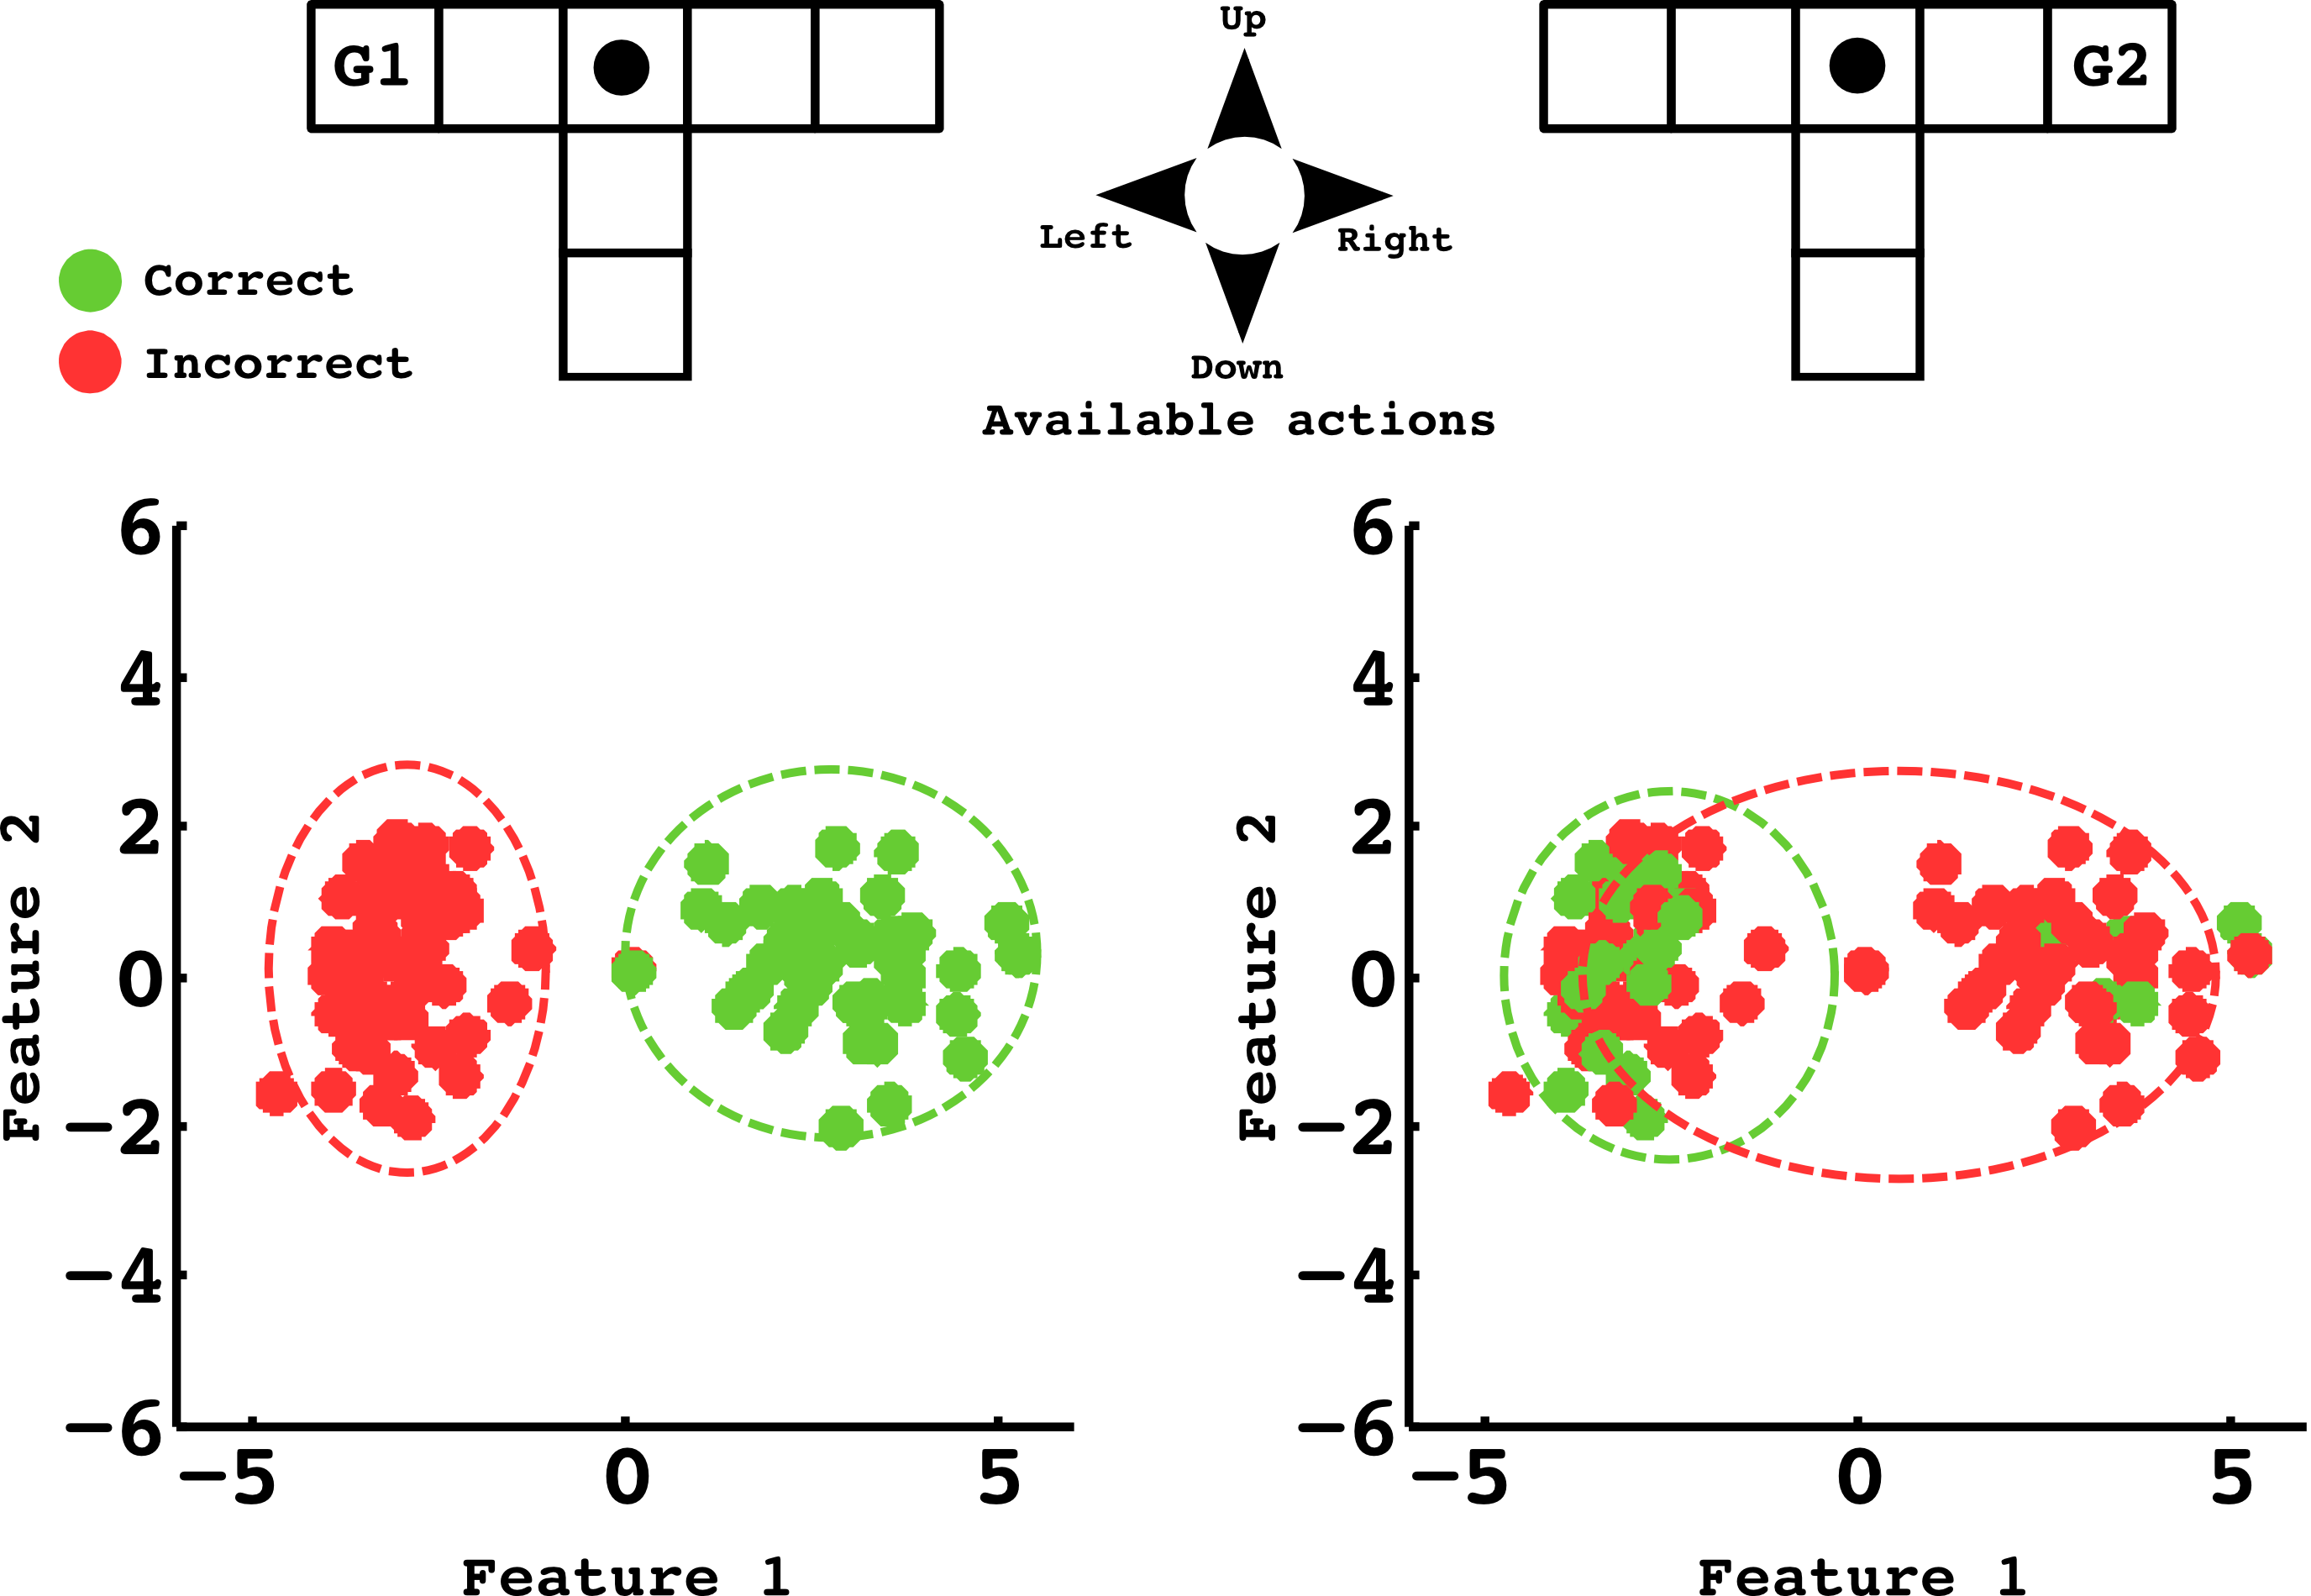
\includegraphics[width=\tworldsize\columnwidth]{\visualspdf/tuto_feedback/Tworld_feedback_labeled_all_actions_with_gaussians.pdf}
    \caption{Interpretation hypotheses made by the agent according to G1 and G2 after many interaction steps. For each class, we compute a Gaussian distribution shown as a dotted line (approximated by hand). The teacher wants the agent to reach G1. The agent is acting randomly. The labels associated to the task G1 are more coherent with the spacial organization of signals in the feature space. It can be measured by the difference in classification performances made by each Gaussian classifier.}
    \label{fig:TworldLabelGaussian}
\end{figure}

By computing the performance of the resulting classifiers, we can test which hypothesis satisfies better the assumption that the signals can be separated by a quadratic curve. As stated in the previous section~\ref{chapter:lfui:signalproperties}, here the choice of the classifier encodes our hypothesis on the underlying structure of the data.

The following of this section formalizes this idea. Next section presents results on a pick and place robotic scenario where the user provides instructions using speech utterances. We use the term label to refer to the meaning associated to user's signals.

\subsection{Notation}

We consider interaction sessions where a machine can perform discrete actions from a set of available actions $a \in \mathcal{A}$ in an either discrete or continuous state space $s \in \mathcal{S}$. The user, that wants to achieve a task $\hat{\xi}$, is providing instructions to the machine using some specific signal $e$, represented as a feature vector  $e \in \mathbf{R}^d$. The task is sequential meaning it is completed by performing a sequence of actions. The machine do not have access to the task the user has in mind, as well as to the actual meaning of each user's signal. Its objective is to simultaneously identify the task and learn to decode user's signals. To achieve this, it has access to a sequence of triplets in the form $D_M = \{(s_i, a_i, e_i),\ i = 1,\ldots,M\}$, where $s_i$, $a_i$ and $e_i$ represent, respectively, the state, action and instruction signals at time step $i$. $D_M$ represents the history of interaction up to step $M$. The behavior of the machine is determined by the actions $a\in\mathcal{A}$ and the corresponding transition model $p(s'\mid s,a)$.

We assume the system has access to a set of task hypothesis $\xi_1,\ldots,\xi_T$ which includes the task $\hat{\xi}$ the user wants to solve. We assume instruction signals $e$ have a finite and discrete number of meanings $l \in \{l_1, l_2, \ldots, l_L\}$ which we call labels. The machine knows the set of possible labels. We further consider that the agent is given a frame function that given a state $s$, an action $a$ and a task $\xi$ returns a label $l$. We will formalize our algorithm in terms of probabilities, therefore the frame represents the conditional probability of a label given a state, an action, and a task, written as $p(l | s, a, \xi)$.

Given this frame, the history of interaction $D_M$, and the set of possible task $\xi_1,\ldots,\xi_T$, we can generate interpretation hypothesis. For a particular task $\xi$, we can associate a label (or probability of label) to each signal according its associated state and action. For each task, this result is a dataset of signal-label pairs. As there is $T$ task hypothesis, we end up with $T$ hypothetic sets.

We assume that given such one set of signal-label pairs, it is possible to compute one decoder that classifies signals $e$ into labels $l$, which we also call the signal to meaning mapping. The parameters of such a model will be denoted by $\theta$. We formalize the decoder function as the conditional probability of a label given a signal and a set of parameters, written as $p(l|e,\theta)$.

As both the frame and the decoder refers to probabilities of labels, we will use different notation for the labels given by the frame, which we denote $l^f$, and predicted by the classifier, which we denote $l^c$. 

Finally, for a given iteration step $i$, we will subscript our notation with a $i$ referring to the iteration number. $i$ will be the only letter refereeing to iteration numbers. We will abuse notation for labels and $l_i$ will refer to a label at step $i$, e.g. $l^f_i$ is the label given by the frame at iteration $i$. Any other subscripting letter for $l$ will refer to a particular class, e.g. $l_k$ is the $k$ class.

% For each hypothesis, at time $i$, we have several dataset $D_i^{\xi_t}$, which are used to train a classifier parameterized by $\theta_i^{\xi_t}$. Each classifier $\theta_i^{\xi_t}$ represents an interpretation hypothesis of the user given he is trying to instruct the task $\xi_t$.

\subsection{Estimating Tasks Likelihoods}
\label{chapter:lfui:likelihood}

We remind that, to measure the coherence of each interpretation hypothesis, we measure the quality, i.e. the accuracy, of a classifier trained on each hypothetic dataset of signal-label pairs. More precisely, for each interpretation hypothesis, we will compute the probability that every observed signal is correctly classified. We remind that the agent never has access to the true labels of the data, therefore, here, a ``correct'' classification always refers to the hypothetic labels associated to each task.
% In other words, we compute whether or not the classifier computed for the specific state-action pairs is able to separate well the different classes. 

% We assume that the classifier's predictions are independent from the frame's predictions. Therefore t
The probability that one signal is correctly classified is the sum across all labels of the probabilities that a signal is of a given label times the probability that the model classifies it as being of this same label. Given an interaction tuple $(s,a,e)$, a task $\xi$, and a classifier $\theta$, we can compute the probability that the signal $e$ is correctly classified according to the frame as:
%
\begin{eqnarray}
p(l^c = l^f | s, a, e, \theta, \xi) = \sum_{k = 1, \ldots, L} p(l^c = l_k | e, \theta) p(l^f = l_k | s, a, \xi)
\end{eqnarray}
%
where we assume independence between $l^c$ and $l^f$. There exists a dependence between the state-action pair considered $(s,a)$ and the meaning of the signal receive $(e)$, but this relation only exists with respect to the task the user has in mind $\hat{\xi}$, which is unknown to the agent. The role of our algorithm is to identify this task. Therefore when evaluating a signal, our system should not have any a priori about the label of such signal, but only rely on the classifier's prediction.

This equation estimates the joint probability for one iteration step, i.e. given only one interaction tuple $(s,a,e)$, and assuming the classifier is already given. We should now compute the probability that all the labels expected by the frame and all the labels predicted by the classifier match together given the history of interaction and for a hypothesized task. Given the full interaction history $D_M$ up to time step $M$, and a task $\xi_t$, we can infer the expected labels $l^f_{1,\ldots,M, \xi_t}$ associated to the signals $e_{1,\ldots,M}$, and compute the associated classifier represented by the set of parameters $\theta_{M, \xi_t}$.

For clarify, we simplify our notation and remove the $\xi_t$ superscript. It is important for the reader to keep in mind that the robot will never have access to the true intended meaning of the users, therefore, as soon as we infer labels, they are always linked to a hypothesized task. Note that the tuple $(s, a, e)$ are observations independent of the task.

Given the classifier $\theta_M$ associated to the task $\xi_t$ at time step $M$, the probability that every expected and predicted labels match together, which we call the likelihood of the task $\xi_t$, is given by:
%
\begin{eqnarray}
\L(\xi_t) &=& \prod_{i = 1,\ldots,M} p(l^c_i = l^f_i | D_M, \xi_t) \nonumber \\ 
&=& \prod_{i = 1,\ldots,M} \sum_{k = 1, \ldots, L} p(l^c_i = l_k | e_i, \theta_M) p(l^f_i = l_k | s_i, a_i, \xi_t)
\label{eq:matchingoverfitting} 
\end{eqnarray}
%
This equation computes the odds that all the predictions made by the classifier equals the labels used to train this classifier. However, the classifier $\theta_{M}$ is here computed using all the history of interaction including all the pairs $(e_i, l^f_i)$. This is may lead to overfitting problems. For example, if we use a simple nearest neighbor classifier between the provided signal-label pairs, Equation~\ref{eq:matchingoverfitting} will computes a likelihood of 1. Indeed, we train and test on the same dataset. Therefore, we should only estimate the likelihood on signals not used to train the classifier.

What we really want to test is if the system is able to make correct prediction about what the frame will predict for a new, never observed, situation, i.e. a new tuple $(s,a,e)$. One possible option is to incrementally update the likelihood of each task as soon as new data comes in:
%
\begin{eqnarray}
\L_i(\xi_t) &=& p(l^c_i = l^f_i | D_i, \xi_t) ~~ \L_{i-1}(\xi_t) \nonumber \\ 
&=& \left( \sum_{k = 1, \ldots, L} p(l^c_i = l_k | e_i, \theta_{i-1}) p(l^f_i = l_k | s_i, a_i, \xi_t) \right) ~~ \L_{i-1}(\xi_t) 
\label{eq:matchingfilter} 
\end{eqnarray}
%
where $\theta_{i-1}$ is the classifier trained on all the past observations up to time $i-1$ and according to the label generated from task $\xi_t$. And with $\L_{0}(\xi_t)$ being the prior at time 0 (before the experiment start) for the task $\xi_t$, usually uniform over the task distribution.

While this is a good enough option as it will be demonstrated in the remaining of this thesis, it does not use all available information. Indeed, the update that was made at time $i-10$ is now out of date as, at time $i$, we now have $9$ more observation tuples available that may change our classifier. Therefore, it would be better to reassess the performance of the classifier given the full set of observation. To do so, and in order to avoid the problem of overfitting, the classifier should be trained on all data but the one tested. We denote by $\theta_{-i}$ a classifier trained on all data available up to time $M$ but the one of time step $i$. We can now rewrite the likelihood as:
%
\begin{eqnarray}
\L(\xi_t) &=& \prod_{i = 1,\ldots,M} p(l^c_i = l^f_i | D_M, \xi_t) \nonumber \\ 
&=& \prod_{i = 1,\ldots,M} \sum_{k = 1, \ldots, L} p(l^c_i = l_k | e_i, \theta_{-i}) p(l^f_i = l_k | s_i, a_i, \xi_t) 
\label{eq:matching} 
\end{eqnarray}
%
While this equation exhibit minor changes over Equation.~\ref{eq:matchingoverfitting}, it avoids problems of overfitting. However, this Equation quickly becomes computational costly and is unlikely to be usable online in practice. For example, after 100 steps, if just 10 task hypotheses were considered, the system would have to compute 1000 classifiers to update the likelihoods of each task. While for the previous equations (Eq.\ref{eq:matchingoverfitting} and Eq.~\ref{eq:matchingfilter}), if 10 task hypothesis are considered, only 10 classifiers must be computed each step.

Still, this last approach is not taking into account the quality of the classifier itself. The question is of knowing how reliable the predictions of the classifier are. A common method to evaluate the uncertainty on a classifier's predictions is to use a cross-validation procedure to estimate the confusion matrix associated to the classifier. Such confusion matrix allows to infer the conditional probability of one label given the label predicted from the classifier $p(l^{cc} = l_k| l^c = l_q, \theta)$, for every combination of $k$ and $q$ in $1, \ldots, L$. Where $l^{cc}$ is the corrected, or ``temperated'', label predicted by the classifier given our estimates on the quality of the classifier's predictions using the cross validation procedure.

For example, a dummy classifier could predict that any given signal $e$ will have a probability $1$ of being of class $l_1$. This classifier is obviously wrong if there more than two labels in the training dataset, and the cross-validation procedure will capture and quantify the classifier bias. If the training dataset were composed of 2 classes with equal number of samples, the confusion matrix will give us the following information: $p(l^{cc} = l_1| l^c = l_1, \theta) = p(l^{cc} = l_2| l^c = l_1, \theta) = 0.5$. Meaning that when the classifier predicts label $l_1$ there is 50 percent of chances that the true label is $l_1$, and 50 percent that it is actually $l_2$. In other words, the classifier is useless. On the contrary, a perfect classifier, that never makes classification errors will be represented by the following conditional probabilities: $p(l^{cc} = l_1| l^c = l_1, \theta) = p(l^{cc} = l_2| l^c = l_2, \theta) = 1$ and therefore $p(l^{cc} = l_1| l^c = l_2, \theta) = p(l^{cc} = l_2| l^c = l_1, \theta) = 0$.

We include the following measure of uncertainty on the classifier's predictions in Equation~\ref{eq:matching}:
%
\begin{eqnarray}
\L(\xi_t) &=& \prod_{i = 1,\ldots,M} p(l^{cc}_i = l^f_i | D_M, \xi_t) \nonumber \\ 
&=& \prod_{i = 1,\ldots,M} \sum_{k = 1, \ldots, L} p(l^{cc}_i = l_k | e_i, \theta_{-i}) p(l^f_i = l_k | s_i, a_i, \xi_t)
\label{eq:matchingcrossvalidation} 
\end{eqnarray}
%
with:
%
\begin{eqnarray}
p(l^{cc}_i = l_k | e_i, \theta_{-i}) =  \sum_{q = 1, \ldots, L} p(l^{cc}_i = l_k| l^c_i = l_q, \theta_{-i}) p(l^c_i = l_q | e_i, \theta_{-i})
\label{eq:confusion} 
\end{eqnarray}
%
These latter equations capture well the full aspect of the problem. However the computational cost explodes, it would require to train 10000 classifiers after 100 steps, to compute the likelihood of just 10 task hypotheses, and using a 10 fold cross-validation procedure. This is impossible to use in real time and, as for Equation~\ref{eq:matchingfilter}, we will rely on an iterative process to cope with this problem:
%
\begin{eqnarray}
\L_i(\xi_t) &=& p(l^{cc}_i = l^f_i | D_i, \xi_t) ~~ \L_{i-1}(\xi_t) \nonumber \\ 
&=& \sum_{k = 1, \ldots, L} p(l^{cc}_i = l_k | e_i, \theta_{i-1}) p(l^f_i = l_k | s_i, a_i, \xi_t) ~~ \L_{i-1}(\xi_t)
\label{eq:matchingfiltercrossvalidation} 
\end{eqnarray}
%
with:
%
\begin{eqnarray}
p(l^{cc}_i = l_k | e_i, \theta_{i-1}) =  \sum_{q = 1, \ldots, L} p(l^{cc}_i = l_k| l^c_i = l_q, \theta_{i-1}) p(l^c_i = l_q | e_i, \theta_{i-1})
\label{eq:confusionfilter} 
\end{eqnarray}
%
where $\theta_{i-1}$ is the classifier trained on all the past observation up to time $i-1$ and according to the label generated from task $\xi_t$. And with $\L_{0}(\xi_t)$ being the prior at time 0 (before the experiment start) for the task $\xi_t$, usually uniform over the task distribution.

Following this latter equation, at each step, for 10 task hypothesis, and using 10 fold cross-validation to estimate $p(l^{cc} | l^c, \theta_{i-1})$ the system would have to compute 100 classifiers to update the likelihoods of each task.

\transition

To summarize, we described several measures of quality of classifiers. We incrementally included some uncertainty measurements to avoid making too sharp estimates when the classifiers are known to be of unreliable and to avoid problems of overfitting.

% (we will use generic name for the task and the classifier parameter, respectively $\xi$ and $\theta$)

Each term of our pseudo-likelihood is computed from three terms: 
\begin{itemize}
\item $p(l^f|s,a,\xi)$ is the frame function, it represents the probability distributions of the meanings according to a task, the executed action and the current state, i.e. it represent the interaction frame. 
\item $p(l^c | e, \theta)$ is the raw prediction of the classifier $\theta$. 
\item $p(l^{cc} | l^c, \theta)$ encodes which label should be actually recovered by $\theta$. It is the probability that the classifier itself is reliable in its predictions. 
% Intuitively, it models the quality of the model $\theta$.
\end{itemize}

In practice our pseudo-likelihood is maximized in two steps. First, the maximum a posteriori estimate $\theta$ of the classifier is computed, and the term $p(l^{cc} | l^c, \theta)$ is approximated using the confusion matrix associated to the classifier based on a cross validation procedure on the training data. Then, given the classifier and the confusion matrix, the likelihood of the task is evaluated. Finally, the best task $\xi$ should be the one that maximizes the pseudo-likelihood.

% It is the probability that the classifier itself is reliable in its prediction.

Note that the term $p(l^{cc} | l^c, \theta)$ is a global approximation of the uncertainty of classifier's prediction. It considers that the classifier suffer from the same biases for any given signal, i.e. it does not depend on the signal $e$ to be predicted.

% predicted signal follow the same ``rule'' and does not depend on the signal $e$ to be predicted.

% A more precise approach would be to consider a confidence measure on the estimation of each point based on the location of this particular point in the feature space, i.e. $p(l^{cc} | l^c, e, \theta)$. For example, a point that is very close to a bunch of point that all belong to the same class is way more likely to be correctly classified than a point far away from any previously seen point or in the middle of a cloud of point with contradictory labels. For example, Montesano et al. in \cite{montesano2012active} use an algorithm that combines beta–binomial distributions and a non-parametric kernel approach to provide the full distribution for the probability of grasping

\subsection{Decision}
\label{chapter:lfui:confidence}

Using any of the measures described above does not inform us about when our system is confident about which task hypothesis is the correct one. Indeed at every iteration step, the likelihood of one task will be higher that all others. Which criteria should we used to decide when ``higher'' is enough?

The simplest method is to normalize the likelihood estimates to $1$, and considered the resulting value as the probability of each task:
%
\begin{eqnarray}
p(\xi_t) = \frac{\L(\xi_t)}{\sum_{u = 1,\ldots, T} \L(\xi_u)}
\label{eq:probanormalize} 
\end{eqnarray}
%
Given this measure, we can define a probability threshold $\beta$, and, when it exists a $t$ such that $p(\xi_t) > \beta$, we can consider the task $\xi_t$ is the one taught by the user.

This method suffers from one important drawback, it does not scale well with the number of hypotheses. Indeed, the more tasks, the more the differences in likelihood between the best task and the other tasks should be important to reach the defined threshold. Consider for example two cases: \begin{inparaenum}[a)] \item for only two tasks whose respective likelihoods are $[0.45, 0.05]$, their normalized likelihood is $[0.9,0.1]$ \item for four tasks whose respective likelihoods are $[0.45, 0.05, 0.05, 0.05]$, their normalized likelihoods are $[0.75, 0.083, 0.0833, 0.083]$. \end{inparaenum}. While the difference of likelihood between the best task and the other tasks is the same in both condition, the normalization decreases the importance of the first task with respect to the others. By scaling this reasoning to one hundred hypotheses, the normalized likelihood method requires immense likelihood differences to reach the same threshold. Therefore, the normalized likelihood method requires to change the threshold for every scenario depending on the number of tasks considered. 

Comparing the likelihood by pairs is a more robust estimate. Considering the example described above, the first hypothesis was 9 times more likely than all other hypotheses in all conditions (2 or 4 tasks considered). We therefore define $W^{\xi_t}$ as the minimum of pairwise normalized likelihood between hypothesis $\xi_t$ and each other hypothesis:
%
\begin{eqnarray}
W^{\xi_t} = \min_{u~\in~{1, \ldots, T} \smallsetminus \{t\}} \frac{\L(\xi_t)}{\L(\xi_t) + \L(\xi_u)}
\label{eq:probapairwise}
\end{eqnarray}
%
When it exists a $t$ such that $W^{\xi_t}$ exceeds a threshold $\beta \in ]0.5,1]$ we consider task $\xi_t$ is the one taught by the user.

Going back to our previous example: \begin{inparaenum}[a)] \item for only two tasks whose respective likelihoods are $[0.45, 0.05]$, their normalized likelihood is $[0.9,0.1]$ while their minimum pairwise normalized likelihood is $[0.9, 0.1]$ \item for four tasks whose respective likelihoods are $[0.45, 0.05, 0.05, 0.05]$, their normalized likelihoods are $[0.75, 0.083, 0.0833, 0.083]$ while their minimum pairwise normalized likelihood is $0.9, 0.1, 0.1, 0.1]$. \end{inparaenum} With our latter measure $W^{\xi_t}$, we can define a threshold that will hold for every scenario independently of the number of hypothesis.

In our various experiments, both measures will be considered.

\subsection{From task to task}
\label{chapter:lfui:tasttotask}

\begin{figure}[!htbp]
  \centering
  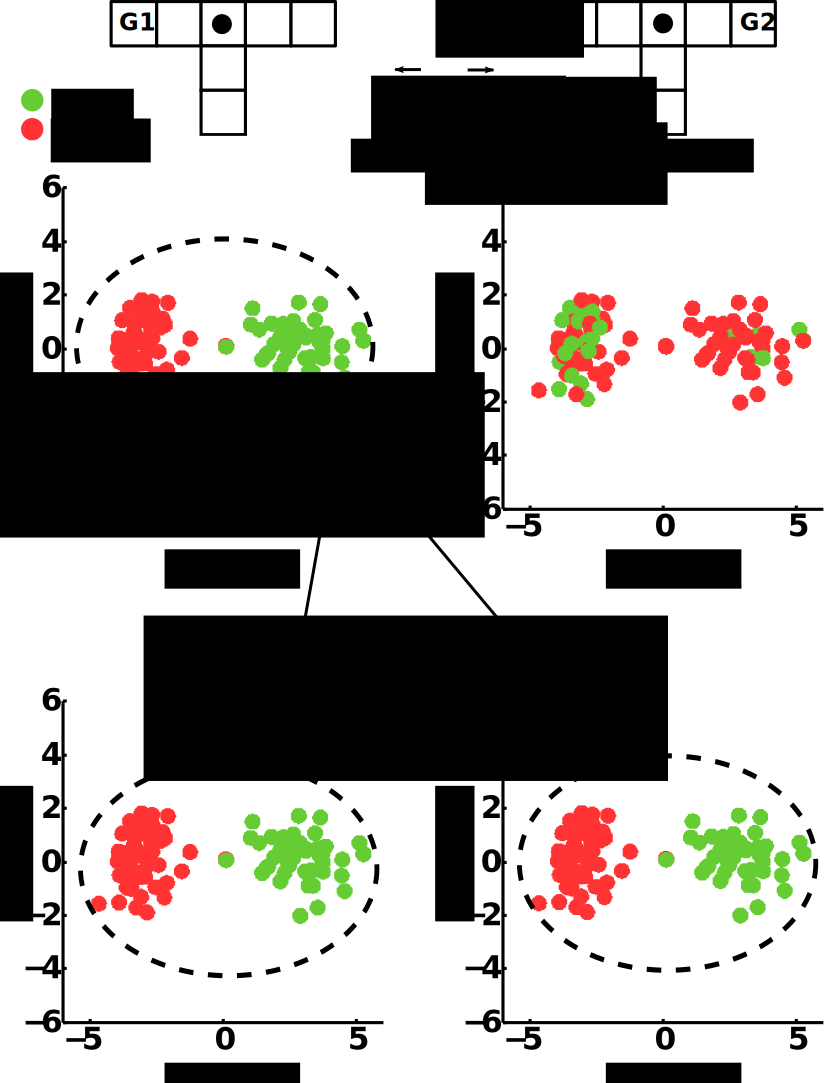
\includegraphics[width=\tworldsize\columnwidth]{\visualspdf/reuse/Tworld_feedback_propagate_labels.pdf}
  \caption{Once a task is identified with confidence, we propagate the labels of the best hypothesis to all the other hypotheses.}
  \label{fig:TworldPropagate}
\end{figure}

Once a task is identified with confidence, the robot executes that task and prepares to receive new instructions from the user according to a new task. Assuming the user starts teaching a new task using the same kind of signals, we now have much more information about the signal to meaning mapping. Indeed, once we are confident that the user was providing instructions related to a specific task, we can infer the true labels of the all the past signals. Therefore we can propagate these labels to all other task interpretation hypothesis (see Figure~\ref{fig:TworldPropagate}), and, by using the same algorithm, we can start learning the new task faster as all hypothesis now share a common set of signal-label pairs. As described in Figure~\ref{fig:TworldReuse}, the signal to meaning models for each hypothesis are still updated every step until the new task is identified and labels reassigned.

\begin{figure}[!htbp]
  \centering
  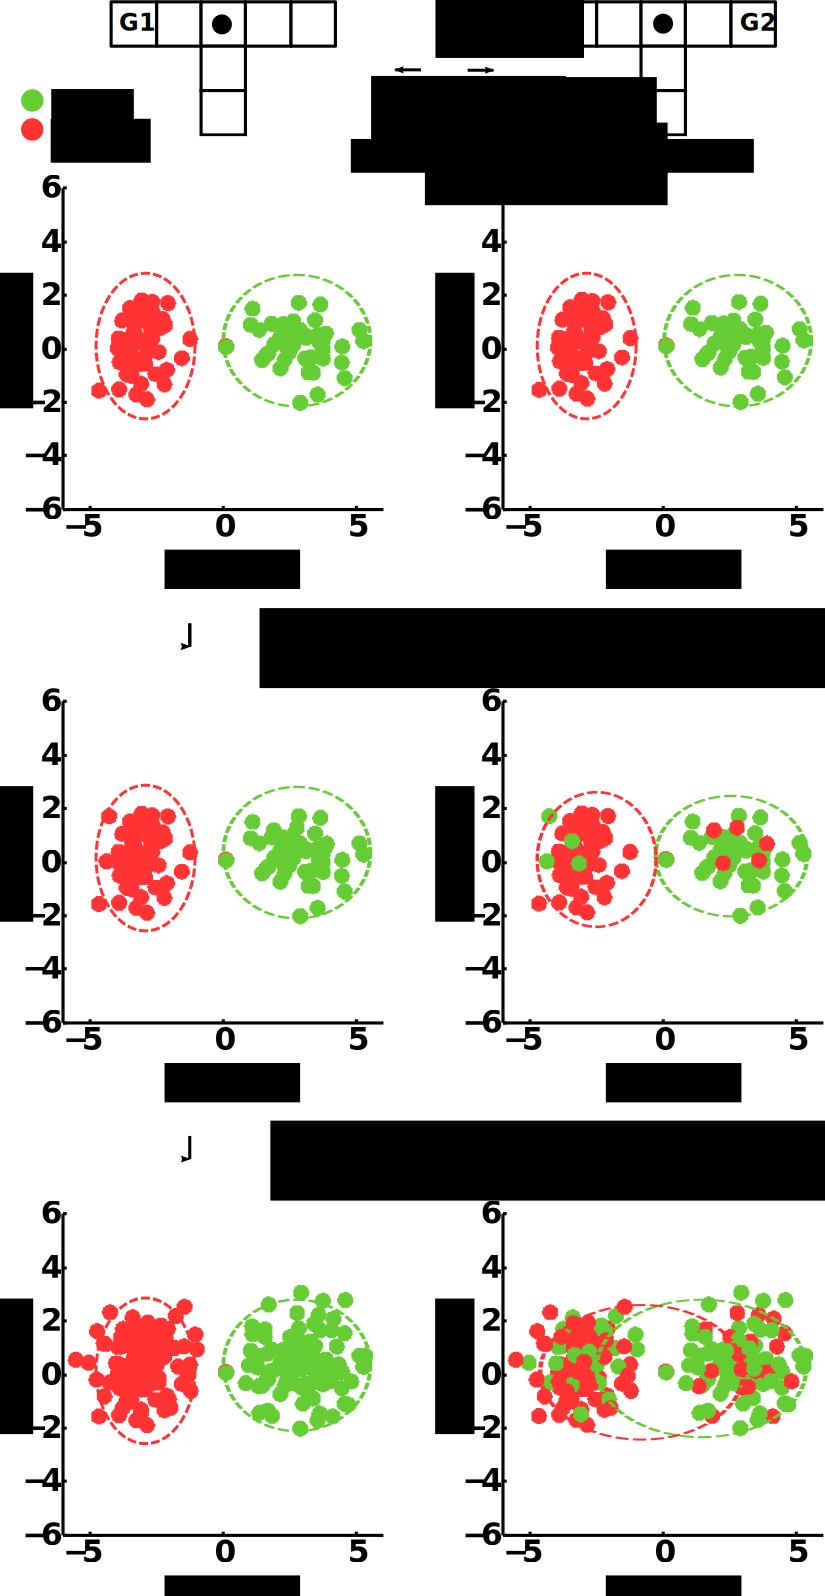
\includegraphics[width=\tworldsize\columnwidth]{\visualspdf/reuse/Tworld_feedback_teaching_again.pdf}
  \caption{When teaching a second task, all hypotheses start with the same signal-label pairs. After a few new interaction steps, some differences in labeling occurs which are easy to detect as they do not conform to the now shared signal model. Therefore allowing to discard quickly the hypothesis G2. We note the interpretation hypothesis process continues to impact the classifiers of each task. The classifier associated to the correct task (here G1) keeps the same quality level, but the one associated to G2 progressively becomes less accurate. This is clearly visible after many steps in the new interaction session.}
  \label{fig:TworldReuse}
\end{figure}

This phase of reuse of previous information could be assimilated to the results of a calibration procedure. Indeed, after a first run we have access to the true intended labels associated to the human signals. The simplest option is therefore to compute one classifier, common all tasks, and to use it to classify new signals.

The method described above differs in that we keep assigning hypothetic labels for each task and we keep updating every classifier. This process allows to decrease the quality of the classifier associated to wrong hypotheses. It helps identifying the correct task faster and more robustly. This effect is more important for the first few task identified. But as the number of signal-label pairs shared between hypothesis increases, the number of new observations needed to sensibly the classifiers increases. Therefore our method progressively converges to the use of a common classifier shared among all hypothesis. This process will be tested in chapter~\ref{chapter:bci} where we will compare our method with a standard calibration procedure approach using EEG signals.

\subsection{Using known signals}
\label{chapter:lfui:known}

In some cases, the robot may already understand some of the communicative signals from the human. For example, the user could have access to two colored buttons, one green to mean ``correct'' and one red to mean ``incorrect''. But the user may prefer using speech to interact with the robot. To allow for flexible interaction, such speech command should not be preprogrammed as each user may speak a different language, or may prefer using the word ``yes'' instead of ``correct'' for example. Considering the mapping between buttons and meanings is known and the mapping between speech utterances and meanings is unknown, we can add a terms to our likelihood equations that includes the information provided by the known signals.

Knowing the meaning of a signal is knowing the parameters $\theta_{button}$ corresponding to the mapping between button presses and their meanings. We can therefore define a separate likelihood update for the known signals, but we simply use the same classifier for each task:
%
\begin{eqnarray}
\L_{button}(\xi_t) &=& \prod_{i = 1,\ldots, M} p(l^{cc}_i = l^f_i | s_i, a_i, e_i, \xi_t, \theta_{button})
\end{eqnarray}
%
The likelihood from the speech can be computed using the equations described in subsection~\ref{chapter:lfui:likelihood}, which we rename $\L_{speech}(\xi_t)$ for convenience.

Finally we can compute the final likelihood as the product of both estimates:
%
\begin{eqnarray}
\L(\xi_t) &=& \L_{button}(\xi_t) ~~ \L_{speech}(\xi_t)
\end{eqnarray}
%
It is important to understand the difference between our approach and a method learning from signals of known meanings. With our approach, we estimate one classifier per task hypothesis. However, if we have access to the true signal to meaning mapping, we must use the corresponding classifier for all hypothesis. Therefore all the equations remain the same, only replacing a global classifier for known signals by hypothetic ones for unknown signals.

\subsection{Two operating modes}

Our algorithm is divided into a classification algorithm, estimating one classifier for each hypothesis based on past interaction, and a filtering algorithm that uses the predictions and properties of this classifier to update a belief over all tasks hypothesis. The key point is that each hypothesis is considered as if it was the true one. We model the signal to meaning mapping of the user with respect to each task. We then simply test if each classifier can make accurate predictions. As the user is acting according to only one hypothesis, only that hypothesis will be able to predict correctly future interactions. Once a task is identified, we have access to the true intended labels of the user. Which we transfer to all the other hypotheses and start learning a new task using the same equation and by continuing the interpretation hypothesis process. As all hypothesis now share a common set of signal-label pairs, we should be able to learn the new task faster.

We highlight the different processes acting during a full experiment when learning multiple tasks. We will refer to two operating modes: \begin{inparaenum}[a)] \item mode 1 is learning the first task from unlabeled instructions, and \item mode 2 is learning a task when most of the labels are shared between hypothesis. \end{inparaenum} Our update equation is the same for the two operating modes but different properties are more or less active during mode 1 or mode 2.

Mode 1 is the main contribution of this work. During mode 1 our measure of uncertainty on classifiers' predictions has more impact than the raw predictions of each classifier. Indeed, with very few data available, the classifiers are unable to predict correctly unseen data. Therefore all classifiers are considered as unreliable, and our update equation makes only small updates each step. It is only once one classifier stands apart as being more reliable than the others that differences between likelihoods will emerges. 

Mode 2 is almost the contrary. Once many tasks have been identified, all hypothesis share a similar classifier because of the transfer of labels. Therefore they all have similar confusion matrix and make similar predictions. Mode 2 is therefore similar to learning from a known source of information, where all tasks share the same classifier. And it is only by comparing the label prediction of new signals to their expected label for each task that we differentiate hypotheses. This process is logically faster than mode 1 because strong updates are made for each received signal.

Between mode 1 and mode 2 is a period of transition where the effects of both modes are active. When only few signal-label pairs are shared between hypotheses, each classifier evolves quickly as new observations come in. 

To sum up, the same processes are active in both modes and are captured by the same equation (see Equation~\ref{eq:matchingcrossvalidation}). In mode 1, it is the classifier intrinsic quality that has the most impact. In mode 2, it is the classification of each individual signal that has the most impact. 

This dynamics may be hard to visualize yet. It will be reminded and illustrated in chapter~\ref{chapter:bci}, where we display the evolution of classification rate of all classifier during an experiment where an agent learn several tasks in a raw. Mode 1 will be observed on Figure~\ref{fig:sequence_evolution} (top), where, during the learning of the first task, all classifier have accuracy close to random (50\%). It is only at step 83 that the correct hypothesis stands apart by being consistently more reliable than the other. Mode 2 will be observed on Figure~\ref{fig:sequence_evolution} (top), where, after the step 200, the difference between classifier qualities is very small. Indeed, 5 tasks have already been identified and all hypotheses share most of their signal-label pairs, therefore all classifiers make similar predictions. The transition between mode 1 and mode 2 will be observed on Figure~\ref{fig:sequence_evolution} (top) between step 83 and 200.

\transition

In next sections, we present results from our algorithm considering a pick and place robotic scenario where a human wants a robot to build a specific structure with cubes and provides instructions to the robot using vocal commands, whose meaning are unknown to the robot at start. We present results both in simulation and with a real robotic system where we test different aspects: \begin{inparaenum}[(a)] \item how our algorithm scale to a robotic scenario considering a feedback frame, \item how it behaves for the case of guidance words, \item the combining of unlabeled signals with signals of known meanings (buttons), \item the reuse of a learned signal-to-meaning mapping for the learning of a new task. \end{inparaenum}

%%%%%%%%%%%%%%%%%%%%%%%%%%%%%%%%%%%%%%%%%%%%%%
%%%%%%%%%%%%%%%%%%%%%%%%%%%%%%%%%%%%%%%%%%%%%%
%%%%%%%%%%%%%%%%%%%%%%%%%%%%%%%%%%%%%%%%%%%%%%
%%%%%%%%%%%%%%%%%%%%%%%%%%%%%%%%%%%%%%%%%%%%%%
%%%%%%%%%%%%%%%%%%%%%%%%%%%%%%%%%%%%%%%%%%%%%%
\section{Method}

We construct a small size pick-and-place task with a real robot. This robot is going to be programmed using a natural speech interface whose words have an unknown meaning and are \textbf{not} transformed into symbols via a voice recognizer. The robot has a prior knowledge about the distribution of possible tasks.

The interaction between the robot and the human is a turn taking, the robot performs an action and waits for a feedback, or guidance, instruction to continue. This allows to synchronize a speech wave with its corresponding pair of state and action. The experimental protocol is summarized in figure \ref{fig:lfui:bloc}.

\begin{figure}[!htbp]
  \centering
  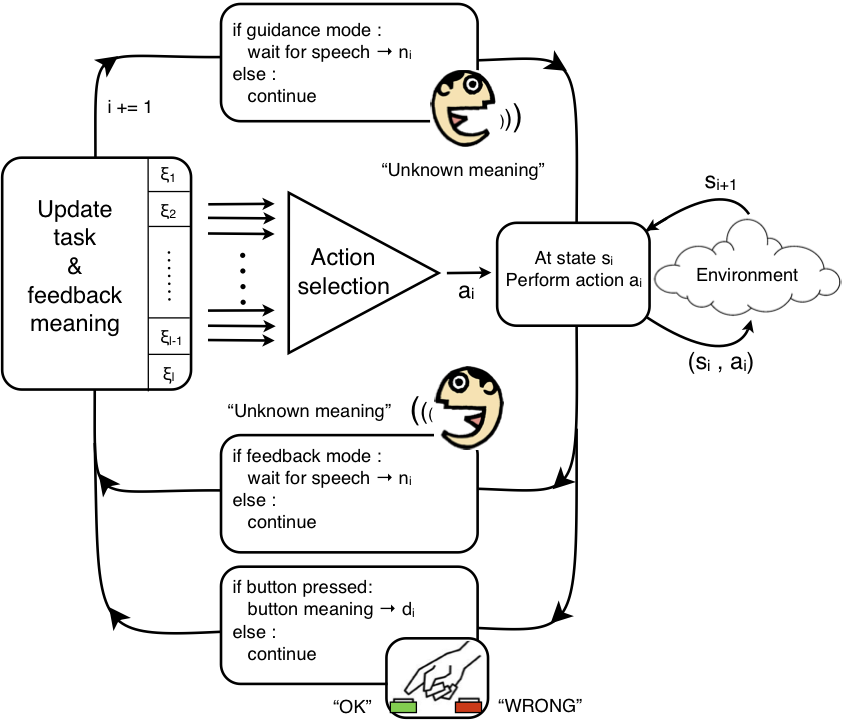
\includegraphics[width=0.6\columnwidth]{\imgpath/bloc.png}
  \caption{Experimental protocol showing the interaction between the teacher and the learning agent. The agent has to learn a task and the meaning of the instructions signals provided by the user, here recorded speech. The teacher can use guidance or feedback signals, and may also have access to buttons of known meanings for the robot.}
  \label{fig:lfui:bloc}    
\end{figure}

\subsection{Robotic System}

We consider a six d.o.f. robotic arm and gripper that is able to grasp, transport and release cubes in four positions. We used a total of three cubes that can form towers of at most two cubes.  The robot has 4 actions available: \textit{rotate left}, \textit{rotate right}, \textit{grasp cube} and \textit{release cube}. The state space is discrete and defined as the location of each object, including being on top of another object or in the robot's gripper. For a set of 3 objects we have 624 different states. Figure~\ref{fig:lfui:setup} shows the robot grasping the orange cube. 

\begin{figure}[!htbp]
  \centering
  \includegraphics[width=0.5\columnwidth]{\imgpath/setup.png}
  \caption{The six d.o.f robotic arm and gripper learning to performing a pick-and-place task with three cubes.}
  \label{fig:lfui:setup}
\end{figure}

\subsection{Task Representation}

We assume that for a particular task $\xi$ we are able to compute a policy $\pi$ representing the optimal actions to perform in every state. One possibility is to use \textit{Markov Decision Processes} (MDP) to represent the problem \cite{sutton1998reinforcement}. From a given task $\xi$ represented as a reward function we can compute the corresponding policy using, for instance, Value Iteration \cite{sutton1998reinforcement}. In any case, our algorithm does not make any assumption about how tasks are represented.

For this particular representation, we assume that the reward function representing the task taught by the human teacher is sparse. In other words, the task is to reach one, yet unknown, of the 624 states of the MDP. Therefore we can generate possible tasks by sampling sparse reward functions consisting of a unitary reward in one state and no reward in all the other.

\subsection{Feedback and Guidance Model}
\label{chapter:lfui:framemodels}

From a given task $\xi$, we can compute the corresponding policy $\pi_{\xi}$. This policy allows to interpret the teaching signals with respect to the interaction protocol defined. In this experiment, we will consider the user is providing either feedback or guidance on the agent's actions. 

\paragraph{} For the feedback case, we define $p(l^f |s,a,\xi)$ as:
%
\begin{equation}
    p(l^f = \emph{correct} |s,a,\xi) = 
    \begin{cases}
    1-\alpha               & if~a = \argmax_a \pi_{\xi}(s,a)\\
        \alpha             & \text{otherwise}\\
   \end{cases}
   \label{eq:feedbackframe}
\end{equation}
%
with $\alpha$ modeling the expected error rate of the user and $p(l^f = wrong |s,a,\xi) = 1 - p(l^f = correct |s,a,\xi)$.

\paragraph{} For the guidance case, the user instructions represent the next action the robot should perform, therefore it only depends on the current state of the robot and the task considered. In our scenario, there are 4 different possible actions ($nA = 4$) in each state. We define $p(l^f |s, \xi)$ for each action as:
%
\begin{equation}
    p(l^f = a |s,\xi) = 
    \begin{cases}
        1-\alpha & if~a = \argmax_a \pi_{\xi}(s,a)\\
        \frac{\alpha}{nA-1} & \text{otherwise}\\
   \end{cases}
   \label{eq:guidanceframe}
\end{equation}
%
with $\alpha$ modeling the expected error rate and assuming only one action is optimal. As the agent can perform 4 different actions, we used the constant $\frac{\alpha}{3}$ for non-optimal actions in order to conserve the property that $\sum_a p(l^f = a |s,\xi) = 1$. For those cases where there is more than one optimal action, the probability is uniformly splitted among them. If all actions are optimal, they all share the same probability of $\frac{1}{nA}$.

\paragraph{} It is important to remember that these frames, while capturing a realistic interaction protocol, are arbitrary and we explicitly ask the users to conform to them. Here we assume that the teacher is aware of the optimal policies to fulfill the task, and additionally shares the same representation of the problem than the robot. Especially, for the scenario considered, the user should be aware that the robot cannot move from position 1 to position 4 in one action. The robot should rather pass thought all intermediate positions $(1 \rightarrow 2 \rightarrow 3 \rightarrow 4)$. However as we known the user will sometime make teaching mistakes, we added a noise term $\alpha$ that account for unpredictable teaching mistakes. For all following experiments $\alpha$ was set to 0.1.

\subsection{Speech Processing}
\label{chapter:lfui:speechdata}

We consider speech as the modality for interacting with the robot. After each action we record the teaching word pronounced by the user. This data is mapped into a 20 dimensional feature space using the methodology described next.  

A classical method for representing sounds is the \textit{Mel-Frequency Cepstral Coefficients} (MFCC) \cite{zheng2001comparison}. It represents a sound as a time sequence of MFCC vectors of dimension 12. Comparing sounds is done via \textit{Dynamic Time Warping} (DTW) between two sequences of feature vectors \cite{sakoe1978dynamic}. This distance is a measure of similarity that takes into account possible insertions and deletions in the feature sequence and is adapted for comparing sounds of different lengths. Each recorded vocal signal is represented as its DTW distance to a base of 20 pre-defined spoken words, which are \textbf{not} part of words used by the teacher.

By empirical tests on recorded speech samples, we estimate that a number of 20 bases words were sufficient and yet a relatively high number of dimensions to deal with a variety of people and speech. This base of 20 words has been randomly selected and is composed of the words:\emph{ \footnotesize{Error, Acquisition, Difficulties, Semantic, Track, Computer, Explored, Distribution, Century, Reinforcement, Almost, Language, Alone, Kinds, Humans, Axons, Primitives, Vision, Nature, Building}}.

% \subsection{Classification System for the Instruction Model}
\subsection{Classifiers}

Any machine learning algorithm working for classification problems can be used in our system. This classifier should be able to generalize from the data and should have appropriate underlying assumptions on the structure of those data. In other words, if the labels were known, the classifier should able to find a good mapping between the signals and their meanings. The only required characteristic is the ability to output a probability on the class prediction, i.e. $p(l|e, \theta)$.

In this study we decided to compare three classifiers:
\begin{itemize}
\item Gaussian Bayesian Classifier (also called quadratic discriminant analysis (QDA)): Computing the weighted mean $\mu$ and covariance matrix $\Sigma$, the usual equations for Gaussian mixture hold.
\item Support Vector Machine (SVM): Using a RBF kernel with $\sigma = 1000$ and $C = 0.1$. The parameter values have been estimated via a swap of parameters and by estimating performances via a cross validation procedure on the dataset. For SVM probabilistic prediction refer to \cite{platt1999probabilistic}.
\item Linear Logistic Regression: The predictive output value ($[0,1]$) is used as a probability measure.
\end{itemize}

Our classifiers are tested on our labeled speech dataset in order to verify their adequacy to model the signal to meaning mapping. All three classifiers obtain accuracy close to 100 percent. This is a rather optimal scenario, we will see in next chapter~\ref{chapter:planning:results} how our algorithm behaves with data of poorer quality.

\subsection{Action selection methods}

% As different sampling methods can lead to different learning behaviors w

The selection of the robot's actions at runtime can be done in different ways. We will compare two different methods: random and  $\epsilon$-greedy. When following random action selection the robot does not use its current knowledge of the task and randomly selects actions. Whereas with $\epsilon$-greedy method the robot performs actions according to its current belief on the tasks, i.e. it follows the policy corresponding to the most likely task hypothesis. The corresponding optimal action is chosen with $1-\epsilon$ probability, otherwise, a random action is selected. In our experiment, we only consider results with $\epsilon =  0.1$.

It is only in the next chapter that we will investigate how the robot can actively selects its future actions in order to improve its performances.

\transition

Before presenting the results of our experiments, we illustrate in next section the pick and place scenario as well as the results of the labeling process for the feedback and guidance case.

%%%%%%%%%%%%%%%%%%%%%%%%%%%%%%%%%%%%%%%%%%%%%%
%%%%%%%%%%%%%%%%%%%%%%%%%%%%%%%%%%%%%%%%%%%%%%
%%%%%%%%%%%%%%%%%%%%%%%%%%%%%%%%%%%%%%%%%%%%%%
%%%%%%%%%%%%%%%%%%%%%%%%%%%%%%%%%%%%%%%%%%%%%%
%%%%%%%%%%%%%%%%%%%%%%%%%%%%%%%%%%%%%%%%%%%%%%
\section{Illustration of the pick and place scenario}
\label{chapter:lfui:pickplace}

We illustrate in Figure~\ref{fig:lfui:pickplaceworld} the pick and place world (where we used balls instead of cubes). There are three objects that can be moved in four different positions and stacked on two levels maximum. The robot's gripper can only grasp the object on top of the stack. An object is always released on top of a stack, except if the stack is full, in which case the release action produces no effect.

\begin{figure}[!htbp]
  \centering
  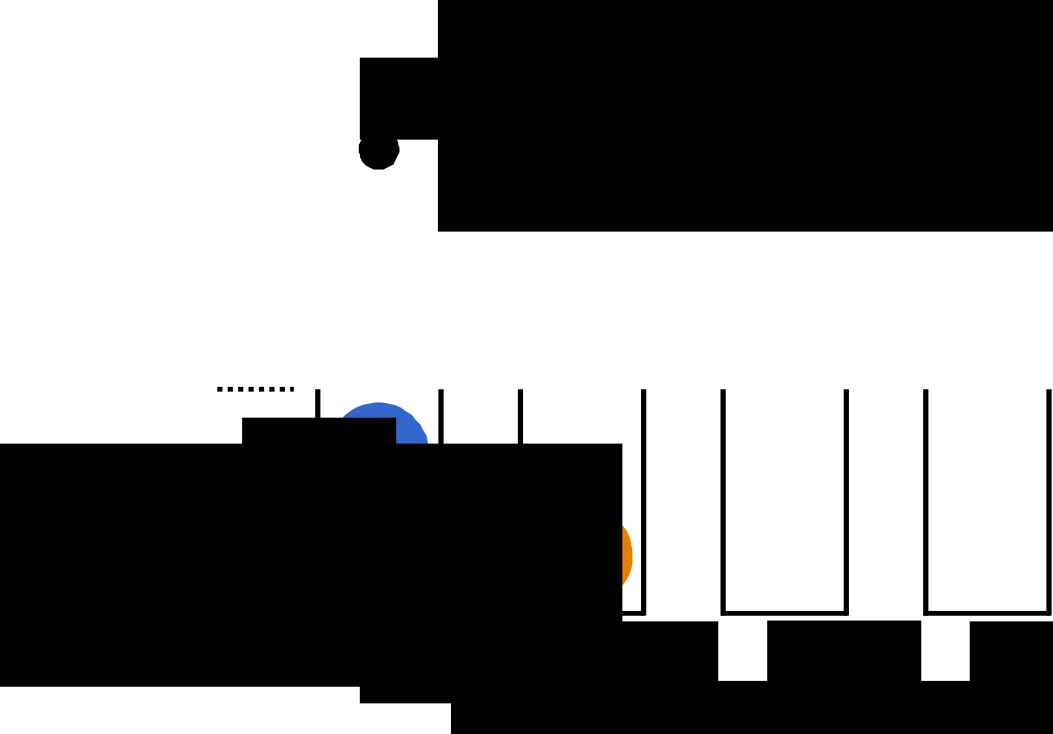
\includegraphics[width=0.4\columnwidth]{\visualspdf/pick_and_place/pick_and_place_world.pdf}
  \caption{A schematic view of the pick and place problem. There is three objects that can be moved in four different positions and stacked on two levels maximum. The robot's gripper can only grasp the object on top of the stack. An object is always released on top of a stack, except if the stack is full, in which case the release action produces no effect.}
  \label{fig:lfui:pickplaceworld}
\end{figure}

In order to complete a task, i.e. to reach a specific configuration of cubes, the robot must perform an ordered sequence of actions. For illustration purpose, we only consider 3 out of the 624 possible hypotheses. Figure~\ref{fig:lfui:pickplacesequence} shows a sequence of actions starting in our hypothesis 1 configuration and going to our hypothesis 3 configuration using the shortest possible number of actions. Hypothesis 2 is a state on this path. While hypothesis 1 and hypothesis 3 seems ``close'' in terms of position of the cubes, they are actually ``far'' one from the other in terms of the action sequence.

\begin{figure}[H]
  \centering
  \includegraphics[width=\columnwidth]{\visualspdf/pick_and_place/pick_and_place_sequence.pdf}
  \caption{A pick and place sequence showing three hypotheses and the sequence of actions from hypothesis 1 to hypothesis 3 through hypothesis 2. While hypothesis 1 and hypothesis 3 seems ``close'' in terms of position of the cubes, they are actually ``far'' one from the other in terms of the action sequence.}
  \label{fig:lfui:pickplacesequence}
\end{figure}

If the user is delivering feedback signals, the labeling process is presented in Figure~\ref{fig:lfui:pickplacefeedback} for a robot acting randomly in the environment. Note that hypothesis 1 and 2 are the most difficult to discriminate by acting randomly as they share most of their optimal policies.

\begin{figure}[H]
  \centering
  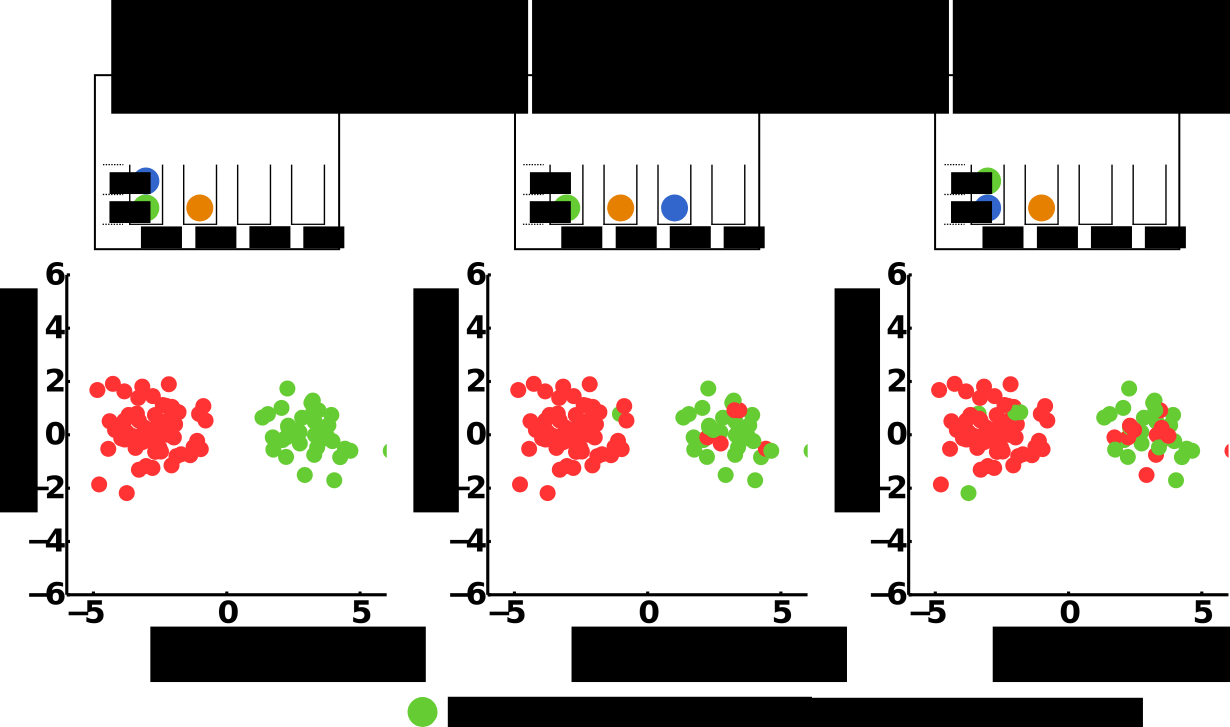
\includegraphics[width=\columnwidth]{\visualspdf/pick_and_place/pick_and_place_feedback.pdf}
  \caption{Results of the labeling process for our three hypotheses and considering the feedback frame. The robot explores randomly the state space. The teacher provides feedback with respect to hypothesis 1. Only a few state-action pairs allowed to differentiate between hypothesis 1 and 2.}
  \label{fig:lfui:pickplacefeedback}
\end{figure}

For the guidance case, the teacher uses the signals presented in Figure~\ref{fig:lfui:pickplaceguidancesignals} and the labeling process is presented in Figure~\ref{fig:lfui:pickplaceguidance} for a robot action randomly in the environment. Note that for some states there may be two optimal actions. For example, in Figure~\ref{fig:lfui:pickplacesequence}, for inverting two stacked cubes there is two different optimal policies, either the one presented in Figure~\ref{fig:lfui:pickplacesequence}, or putting the blue ball in position 2 and the green in position 3 during the exchange of position. These equally optimal options make the learning process more difficult, we can still visually find out that for hypothesis 1 all points in each cluster share one color, which is not the case for the other two hypotheses.

\begin{figure}[H]
  \centering
  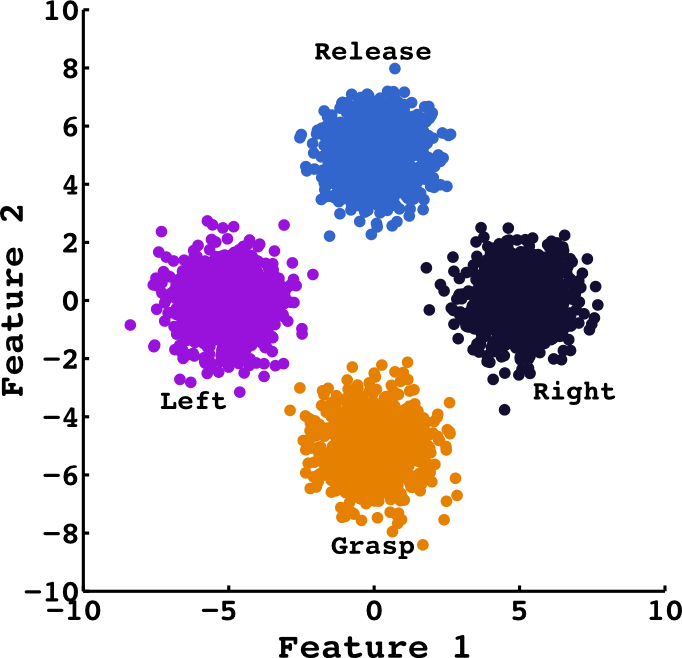
\includegraphics[width=\signalwidth\columnwidth]{\visualspdf/pick_and_place/guidance_pick_and_place.pdf}
  \caption{The guidance signals used for our visual example.}
  \label{fig:lfui:pickplaceguidancesignals}
\end{figure}

\begin{figure}[H]
  \centering
  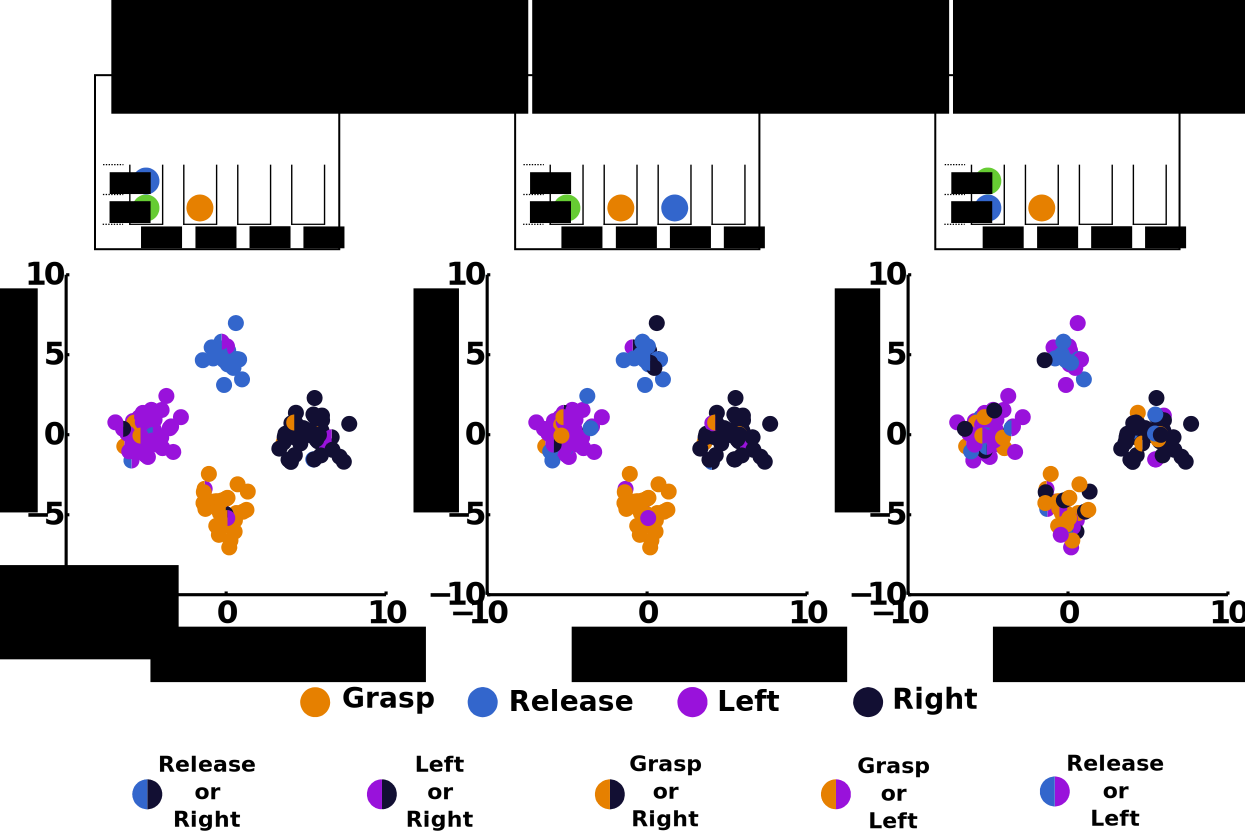
\includegraphics[width=\columnwidth]{\visualspdf/pick_and_place/pick_and_place_guidance.pdf}
  \caption{Results of the labeling process for our three hypotheses considering the guidance frame. The robot explores randomly the state space. The teacher provides guidance with respect to hypothesis 1. The labeled signals that contain two colors represent situations where the user could have given two different guidance signals, i.e. where two actions were optimal. It is only for hypothesis 1 that all signals in each cluster share one color. The case of guidance with multiple optimal actions in some states makes the learning process more ambiguous and may require some additional time compared to the feedback case.}
  \label{fig:lfui:pickplaceguidance}
\end{figure}

\visuopti{\newpage}

% \transition

We have provided an example of the pick and place world with two dimensional signals and considering only three hypotheses. In next section, we consider real spoken words mapped to a 20 dimensional space and the full space of hypothesis consisting of 624 possible object configurations.

%%%%%%%%%%%%%%%%%%%%%%%%%%%%%%%%%%%%%%%%%%%%%%
%%%%%%%%%%%%%%%%%%%%%%%%%%%%%%%%%%%%%%%%%%%%%%
%%%%%%%%%%%%%%%%%%%%%%%%%%%%%%%%%%%%%%%%%%%%%%
%%%%%%%%%%%%%%%%%%%%%%%%%%%%%%%%%%%%%%%%%%%%%%
%%%%%%%%%%%%%%%%%%%%%%%%%%%%%%%%%%%%%%%%%%%%%%
\section{Results}
\label{chapter:lfui:results}

The experiments presented in this section follow the protocol described in figure~\ref{fig:lfui:bloc}, where each turn the agent performs one action and waits for the teaching signals from the teacher. We first present a set of simulated experiments using the same MDP as for the real world experiment. We start by assuming that the teacher provides feedback instructions without any mistakes. % , therefore only the noise inherent to the spoken signals remains. 
We compare first the different classifiers, and then the performances of $\epsilon$-greedy versus random action selection methods both for the feedback and guidance cases. Later, we present an empirical analysis of robustness to teaching mistakes. The last simulated experiment considers a teacher having also access to buttons of known meaning. Finally, we show a result using the real robot and a human user, where we study how signals knowledge learned in a first run can be used in a second one to learn more efficiently.

In order to be able to compute statistically significant results for the learning algorithm, we created a database of speech signals that can be used in simulated experiments. All results report averages of 20 executions of the algorithm with different start and goal states. 

As there are 624 hypotheses, we must update 624 likelihoods at each step. Depending on the likelihood equation considered this may not be feasible in real time. As our aim is to run our system in real time, and as we know that the speech signals in our dataset are well separated in their feature space, we use the simplest version of our likelihood estimation methods described in Equation~\ref{eq:matchingoverfitting}. To estimate the probability of each task we normalize the likelihood estimates $\L_(\xi_1),\ldots,\L_(\xi_T)$ to 1.

% The interested reader will find in appendix~\ref{appendix:pickplace} an illustration of the pick and place world as well as the results of the labeling process for the feedback and guidance case.

\subsection{Learning feedback signals}

In this experiment, the teacher is providing spoken signals whose meanings are either ``correct'' or ``incorrect''. The robot should simultaneously learn the task and the mapping between the spoken words and the binary meanings. The action selection of the robot is done using the $\epsilon$-greedy method. The user uses only one word per meaning.

The results comparing the different classification methods are shown in Figure~\ref{fig:FeedbackOneWord}. It shows the evolution of the probability associated to the task the teacher has in mind. We can track this information because we know, as experimenters, the true task taught by the teacher. Note that after 200 iterations all three classification methods identified the correct task as the most likely, i.e. the normalized likelihood values of the correct task are greater than 0.5, meaning that the sum of all the others is inferior to 0.5. Logistic regression provides the worse results in terms of convergence rate and variance.

\begin{figure}[!htbp]
  \centering
  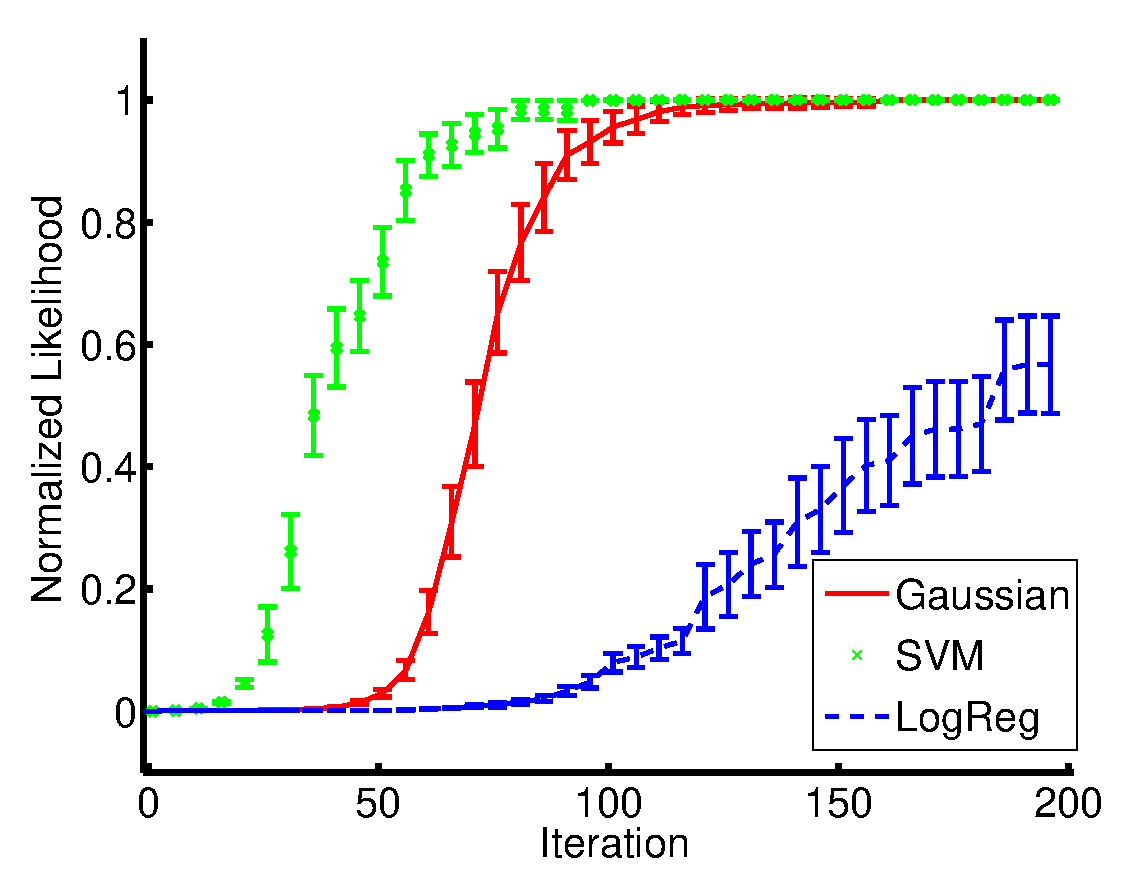
\includegraphics[width=\plotsize\columnwidth]{\imgpath/classifiers}
  \caption{Taught hypothesis normalized likelihood evolution (mean + standard error) thought iterations using different kinds of classifiers. The teacher is providing feedback signals using one word per meaning and the agent is performing actions according to the $\epsilon$-greedy strategy.}
  \label{fig:FeedbackOneWord}
\end{figure}

The user is not restricted to the use of only one word per meaning. Table~\ref{tab:1} compares the taught task normalized likelihood value after 100 iterations for feedback signals composed of one, three and six spoken words per meaning. SVMs have better performances when using one word per meaning but the Gaussian classifier has overall better results with less variance, see Table~\ref{tab:1}.

\begin{table}[!htbp]
\centering
\begin{tabular}{|l|c|c|c|}
\hline
&\textbf{One word}&\textbf{Three words}&\textbf{Six words}\\\hline
\textbf{Gaussian}&1.0 (0.1)&1.0 (0.1)&0.7 (0.1)\\\hline
\textbf{SVM}&1.0 (0.0)&0.5 (0.4)&0.3 (0.4)\\\hline
\textbf{LogReg}&0.1 (0.1)&0.2 (0.3)&0.2 (0.3)\\\hline
\end{tabular}
\caption{Taught hypothesis normalized likelihood values after 100 iterations (mean and standard deviation). Comparison for different classifiers and number of words per meaning. The Gaussian classifier has overall better performances.}
\label{tab:1}
\end{table}

Interestingly the Gaussian classifier learns better after 100 iterations than the other classifiers with many words per meaning. This counter intuitive result can be explains by the high dimensionality of the space where even one Gaussian can differentiate several groups of clusters. Linear logistic regression has lower performance presumably due to the linear decision boundary. For the SVM classifier, which is kernalized, as only 100 data points are distributed between each cluster, the more the number of clusters increases the less data points belong to each cluster. The fitting process of the SVM is therefore more likely to consider some data as noise, omitting some clusters. For the following experiments, we will only consider the Gaussian classifier, first because it has overall better performance, but also because it is the faster to train and thus is the only one usable for online experiments. 

% Indeed, in this setup, at each iteration the agent has to train 624 classifiers.

\subsection{Learning guidance signals}

In Figure~\ref{fig:Guidance}, we compare the performance between using feedback or guidance signals. From feedback to guidance the number of meanings is increased from two (correct/incorrect) to four (left/right/grasp/release). As depicted in Figure~\ref{fig:Guidance}, the robot is able to identify the task based on unlabeled guidance signals. However it requires more iterations to reach the same level of confidence. This may look counter intuitive because guidance signals are more informative. However the robot now needs to classify instructions in four different meanings, i.e. to identify four clusters of signals, which requires more samples. 

\begin{figure}[!htbp]
  \centering
  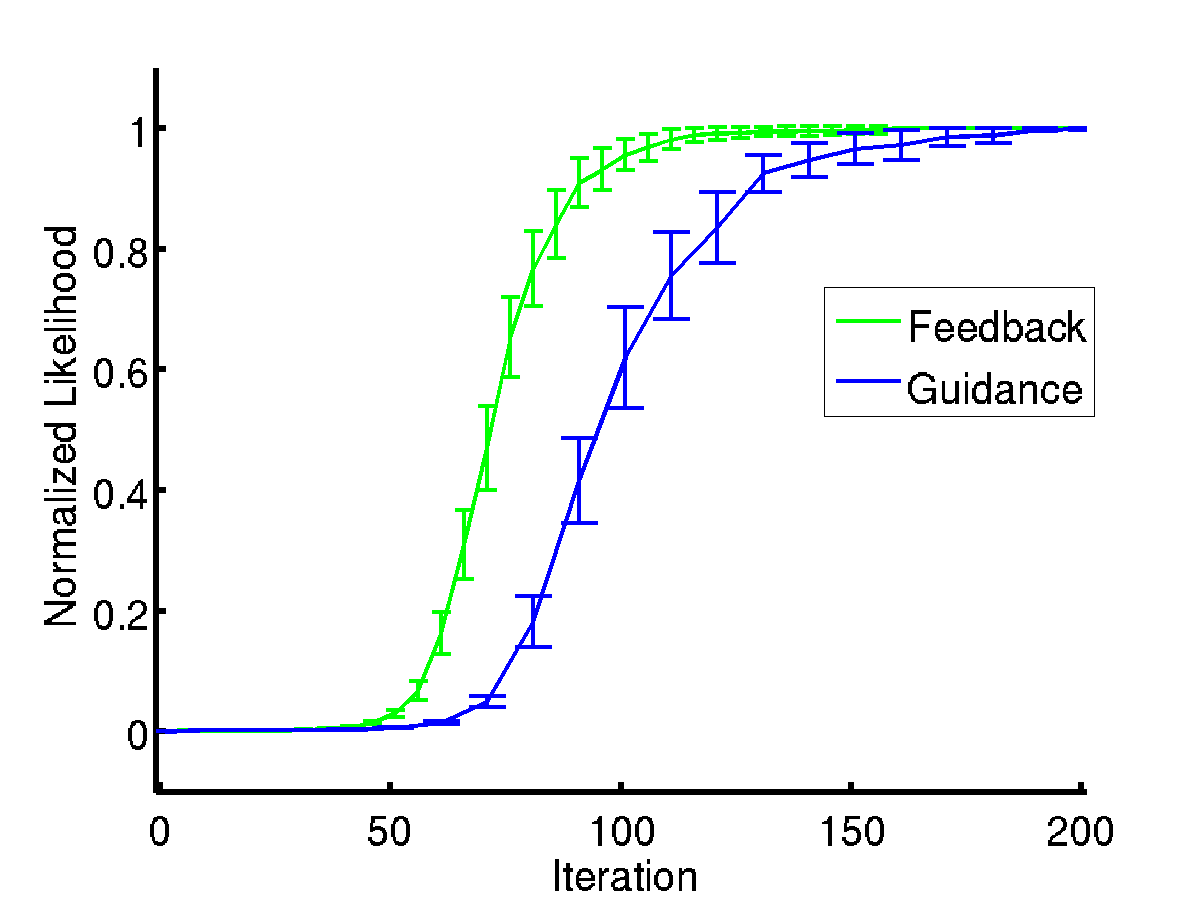
\includegraphics[width=\plotsize\columnwidth]{\imgpath/feedback_vs_guidance}
  \caption{Taught hypothesis normalized likelihood evolution (mean + standard error) thought iterations using Gaussian classifier. Comparison of feedback (green) and guidance (blue) instructions using one word per meaning. The robot is able to learn the task based on both feedback and guidance signals but needs more iterations for the guidance case.}
  \label{fig:Guidance}
\end{figure}

\subsection{Robustness to teaching mistakes}

Until now, we made the assumption that the teacher is providing feedback or guidance signals without any mistake. But in real world scenario, people can fail in providing optimal feedback. This is why we initially included the $alpha$ constant in our frame's equations (see section~\ref{chapter:lfui:framemodels}). An empirical analysis of robustness is shown in figure~\ref{fig:Noise} using feedback signals, Gaussian classifier, and one word per meaning. We compares two ways of training the Gaussian classifiers: \begin{inparaenum}[(1)] \item estimating the maximum likelihood (ML) of the Gaussian for each class, namely the mean and covariance, and \item using the expectation maximization (EM) algorithm \cite{dempster1977maximum} to iteratively update the mean and covariance of each class in order to find the underlying structure of the data. \end{inparaenum} 

% It allows to find the true underlying structure more efficiently.

We show that the EM approach is improving robustness to teaching mistakes. Referring to our previous discussion in section~\ref{chapter:lfui:whynotEM}, note that we initialized the EM algorithm with the ML estimates for each Gaussian, and we kept track which Gaussian belongs to which meaning. In addition, the representation used for the spoken words is of high quality and separates well the signals in the feature space. Therefore it is unlikely for the EM algorithm to fail at finding the two clusters given the data properties.

\begin{figure}[!htbp]
  \centering
  \begin{subfigure}[b]{0.49\columnwidth}
    \centering
    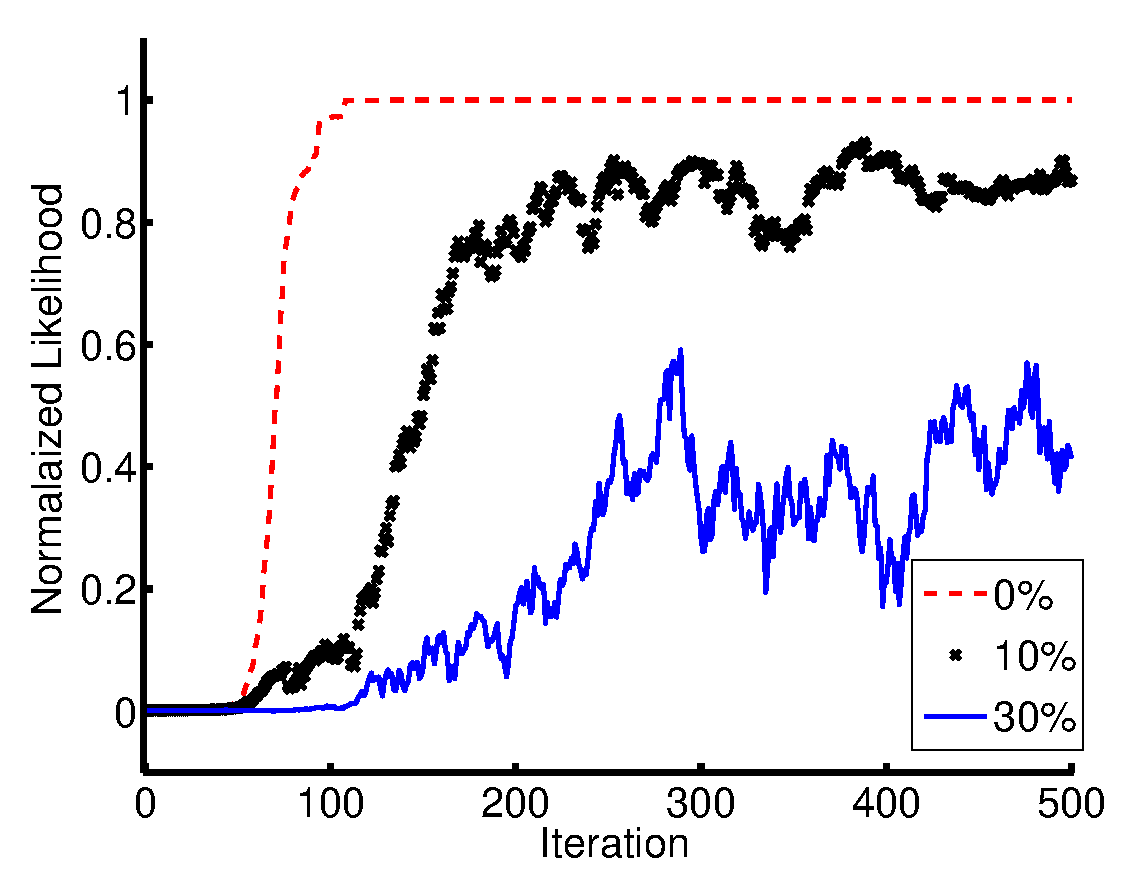
\includegraphics[width=\columnwidth]{\imgpath/noise_no_EM}
    \caption{ML}
  \end{subfigure}
  \begin{subfigure}[b]{0.49\columnwidth}
    \centering
    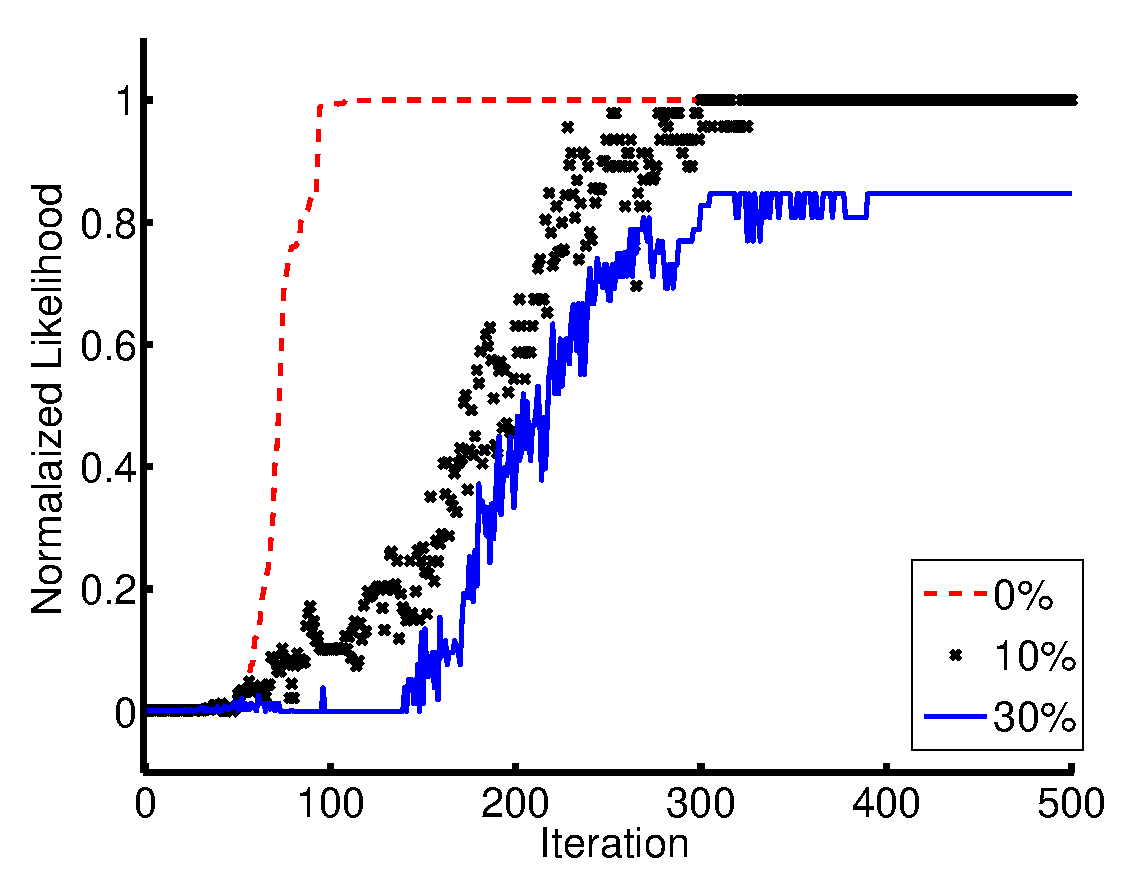
\includegraphics[width=\columnwidth]{\imgpath/noise_with_EM}
    \caption{EM}
  \end{subfigure}
  \caption{Taught hypothesis normalized likelihood evolution thought iterations using Gaussian classifier. Comparison of the ML estimates (left) versus EM estimates (right). The teacher is providing feedback using one word per meaning with different percentage of mistakes. Actions are selected following the $\epsilon$-greedy method. Standard error has been omitted for readability reason.}
  \label{fig:Noise}
\end{figure}

\subsection{Including prior information}
\label{sec:IncludingPriorInformation}

Learning purely from unknown teaching signals is challenging for the researcher but could be restrictive for the teacher. Therefore additional sources of known feedback are consider, such as a green and a red button, where the green button has a predefined association with a ``correct'' meaning, as red button with a ``incorrect'' meaning. 

% Yet, we shall expect that even in this case, users will use more modalities than the predefined one.

In this study, the teacher still provides unlabeled spoken words but can also use the red and green button as described in figure~\ref{fig:lfui:bloc}. However, and in order to avoid the possibility of direct button to signal association, the user can never use both modalities at the same time and use them alternatively with equal probability. Therefore, in average, after 250 iterations the robot has received 125 labeled button presses and 125 unlabeled speech signals. In most systems, the speech signals would be ignored but our method enables learning from the unlabeled signals. We compare three learning methods: \begin{inparaenum}[(1)] \item the robot is learning only via the labeled button presses, \item it uses only the unlabeled speech signals, and \item it uses both labeled and unlabeled signals. \end{inparaenum} Figure~\ref{fig:button} shows results from this setting. 

\begin{figure}[!htbp]
  \centering
  \includegraphics[width=\plotsize\columnwidth]{\imgpath/mix_button}
  \caption{Taught hypothesis normalized likelihood evolution (mean + standard error) thought iterations using Gaussian classifier. Comparison of using known button presses, unknown spoken signals, and both.}
  \label{fig:button}
\end{figure}

As expected, learning from labeled feedback is faster than with unlabeled signals. However taking advantage of different sources of information, even a priori unknown, can led to slightly better performances than using only known information. Importantly, the signals to meaning mapping of speech signals learned during a first task, could later be reused in further interactions.

\subsubsection{Reuse using a real robot}

Statistical simulations have shown that our algorithm allows an agent to learn a task from unlabeled feedback in a limited amount of interactions. To bridge the gap of simulation we tested our algorithm in real interaction conditions with our robotic arm. In this experiment, the teacher is facing the robot and chooses a specific goal to reach (i.e. a specific arrangement of cubes he wants the robot to build). He then decides one word to use as positive feedback and one as negative feedback, and starts teaching the robot. For this experiment the word \textit{``yes''} and \textit{``no''} were respectively used for the meaning ``correct'' and ``incorrect''. 

Once the robot has identified the first task, we keep in corresponding classifier and start a new experiment where the human teacher is going to use the same feedback signals to teach a new task. However the second time, the spoken words are first classified as ``correct'' or ``incorrect'' meaning according to the previously learned classifier. We study here two things, first does our system bridges the reality gap and can we reuse information about the signal to meaning mapping learned from a previous interaction session?

Figure~\ref{fig:Real} shows the result from this setting. In the first run it took about 100 iterations for the robot to identify the task. Whereas in the second run, when reusing knowledge from the first one, the robot is able to learn a new task faster, in about 30 iterations. The second run being faster that the first one indicates that our algorithm identified correctly the mapping between the user's speech signals and their corresponding meanings. 

The author of this thesis was the user for this studies and was therefore aware of the task representation used by the robot, i.e. a MDP with four discrete actions. As explained in subsection~\ref{chapter:related:humanintheloop}, an important challenge is to deal with non-expert humans whose teaching styles can vary considerably. While this challenge is not part of the current study, we observed that non-informed users teaching our robot had various understanding of the robot behaviors. It most often led to unsuccessful interactions due to an important amount of teaching mistakes from non-informed users.

% the two clusters in our $\mathbb{R}^{20}$ dimensional space as well as 

\begin{figure}[!htbp]
  \centering
  \includegraphics[width=\plotsize\columnwidth]{\imgpath/real}
  \caption{Taught hypothesis normalized likelihood evolution thought iterations using Gaussian classifier. A real teacher delivers spoken feedback signals using one word per meaning. The robot uses the $\epsilon$-greedy action selection method. A first run of 100 iterations is performed where the robot learns a task from unknown feedback. Then, by freezing the classifier corresponding to the most likely task, the user teaches the robot a new task.}
  \label{fig:Real}
\end{figure}

% We used a simplified version were the label from the first task are used to calibrate a classifier used for the learning of the second task.

\subsection{Action selection methods}

Finally, we compare the impact of using different action selection methods, we consider the $\epsilon$-greedy and the random action selection methods.

Figure~\ref{fig:selectionMethod} left and right compares respectively the action selection method for the case of feedback and guidance interaction frames. The $\epsilon$-greedy method results in a faster learning with less variance. The $\epsilon$-greedy method leads the robot in the direction of the most probable goal. In this way, the robot will receive more diverse feedback and will visit more relevant states than what a random exploration does.

\begin{figure}[!htbp]
  \centering
  \begin{subfigure}[b]{0.49\columnwidth}
    \centering
    \includegraphics[width=\columnwidth]{\imgpath/feedback}
    \caption{Feedback}
  \end{subfigure}
  \begin{subfigure}[b]{0.49\columnwidth}
    \centering
    \includegraphics[width=\columnwidth]{\imgpath/guidance}
    \caption{Guidance}
  \end{subfigure}
  \caption{Taught hypothesis normalized likelihood evolution (mean + standard error) thought iterations using Gaussian classifier. The teacher is providing feedback (left) or guidance (right) signals using one word per meaning. The $\epsilon$-greedy action selection method allows a faster learning than the random method. Note that the x-axis, showing the number of iterations, does not considered the same range for the feedback (left) and guidance (right) cases.}
  \label{fig:selectionMethod}
\end{figure}

\section{Discussion}

We showed that learning simultaneously a task and the meaning of an a priori unknown human instruction is possible and that the action selection method impacts the learning performances. Can we do better than random or $epsilon$-greedy action selection methods?

% This experiment was performed at a very early stage of this work and was not yet considering the full method introduced in section~\ref{chapter:lfui:tasttotask}.

Using an active learning approach \cite{settles2010active}, it might be more efficient to choose the actions that are expected to reduce the uncertainty as fast as possible. In next chapter, we investigate and detail the specific properties of the uncertainty in our problem, where not only the task is unknown but also the signal to meaning mapping. We will provide measures of uncertainty that can be used as exploration bonuses for exploration strategies. We will finally present results from artificial dataset of different qualities in a two-dimensional grid world scenario.

%%%%%%%%%%%%%%%%%%%%%%%%%%%%%%%%%%%%%%%%%%%%%%
%%%%%%%%%%%%%%%%%%%%%%%%%%%%%%%%%%%%%%%%%%%%%%
%%%%%%%%%%%%%%%%%%%%%%%%%%%%%%%%%%%%%%%%%%%%%%
%%%%%%%%%%%%%%%%%%%%%%%%%%%%%%%%%%%%%%%%%%%%%%
%%%%%%%%%%%%%%%%%%%%%%%%%%%%%%%%%%%%%%%%%%%%%%
% \section{Discussion}

% In this work we presented an interactive learning system that can learn the initially unknown association between unlabeled instruction signals and their meaning while learning a new task. We presented empirical results showing that 1) our system can learn from unknown feedback, unknown guidance instruction signals, or a mixture of these signals, 2) it can recover from teaching mistakes, 3) it can leverage additional known sources of information, and 4) different standard classifiers can be used. An experiment with a real robot and a real user showed that 5) it can reuse acquired knowledge about human instruction signals in the learning of a new task. Finally we presented an extended experiment that mixed unknown feedback and guidance instructions, in a continuous environment, and showed that 6) an uncertainty based planning algorithm, using uncertainty from both task estimation and instruction classification, is the most efficient strategy.

% \subsection{Instruction modalities} Instruction signals were here conveyed using speech sounds (which may have been interjections, or even sounds of clapping or tapping hands). Of particular interest is the possibility to use the same system with multiple modalities for instruction signals, such as facial expressions or hand gestures. This allows different users to use the system according to their own modality preferences, potentially related to their own skills and limitations. In principle, since no part of the system is specific to the sound modality, and since the sound modality is already relatively complex, there are no theoretical obstacles for this experimental extension. An interesting example might be to consider brain-computer interfaces system \cite{chavarriaga2010learning, iturrate2010robot} that usually require a long an explicit training phase. Using our system we would be able to simultaneously understand the meaning of brain signals and what task is the user trying to achieve. We started investigating in that direction with promising preliminary results \cite{grizou2013zero}.


% say that the signal were very easy to classify






% %!TEX root = ../../thesis.tex
\define{\chapterpath}{\allchapterspath/planning}
\define{\imgpath}{\chapterpath/img}

\define{\twoplanningwidth}{0.7}
\define{\threeplanningwidth}{1}
\define{\twotworldsize}{0.8}
\define{\threetworldsize}{1}
\define{\plotsize}{0.6}

\chapter{Planning upon Uncertainty}
\label{chapter:planning}
\minitoc


In previous chapter, we presented our algorithm allowing to solve a task from human instruction signals without knowing in advance the mapping between the signals and their meanings. We have seen seen that the performances of our system is affected by the action selection method used by our robot. In this section we investigate further how the agent should plan its action to improve the learning efficiency. To do so, our agent will look for action that disambiguate between hypothesis, which is the one that reduce the uncertainty about which hypothesis is the correct one.

We start by explaining what should be the method and measure of uncertainty use by a system that has access the the true signal to meaning mapping. We then providing an intuition on what are is the additional sources of uncertainty inherent to our problem, and link it with the problem of symmetries seen in chapter~\ref{chapter:lfui:symmetries}. After this, we propose two ways of estimating the uncertainty in our scenario, one on the signal space and one on the meaning space using hypothetic signals. We finally present simulated experiments showing that our measure of uncertainty allow the robot to plan efficiently its action in order to disambiguate between hypothesis. Those results uses a series of dataset of different qualities and dimensionality, and we will see that the performance of the system are affected by the quality of the data more than their dimensionality. An important aspect of our algorithm is to detect those cases it can not discriminate between task, and for those case where a good classifier can not be found, the algorithm will not select between hypothesis.

On this basis we will transition to chapter~\ref{chapter:bci} which present an application to brain computer interaction scenarios where human users guide an agent on a specific square of a grid using feedback signals and without having to calibrate the brain decoder before hand.

%%%%%%%%%%%%%%%%%%%%%%%%%%%%%%%%%%%%%%%%%%%%%%
%%%%%%%%%%%%%%%%%%%%%%%%%%%%%%%%%%%%%%%%%%%%%%
%%%%%%%%%%%%%%%%%%%%%%%%%%%%%%%%%%%%%%%%%%%%%%
%%%%%%%%%%%%%%%%%%%%%%%%%%%%%%%%%%%%%%%%%%%%%%
%%%%%%%%%%%%%%%%%%%%%%%%%%%%%%%%%%%%%%%%%%%%%%
\section{Uncertainty for known signal to meaning mapping}

If the true mapping between human communicate signals and their meaning is provided to the machine, and that it still has to identify the correct task between a finite set of task and has access to the interaction frame, the learning process is rather trivial. Indeed, in such case, the robot should only compares if what the meaning received from the human match well with what is expected from the given frame and a given task. If they match then we can increase the probability of such task, if they do not match we can decrease the probability.

The robot should therefore seek for the state-action pairs that maximally disambiguate between hypothesis. For example, if for one given state-action pair, half of the hypothesis expect a signal of meaning ``correct'' and the other half expect one of meaning ``incorrect''. By performing this action in that state, the system will rule out half of the hypothesis once the user will have provided its feedback. 

It is important for this process to be weighted by the current probability associated with each task hypothesis. Indeed once we have rules out half of the hypothesis, we should only focus on differentiating the remaining hypothesis. For this the robot should seek for a new state-action pair where the remaining hypothesis will disagree on the expected meaning from the teacher.

But this process is here describe in a way that is not realistic, our robot can not query any state-action pair, it can not teleport but rather should navigate through the all state space to be able to finally perform that state-action pair. And on its way to a specific state-action pair, it may already have received new information changing its current belief on the hypothesis probabilities.

A solution to this problem is to add exploration-bonuses for each state-action pair corresponding to the uncertainty associated to each state-action pair. The agent can then select its next action considering the full map of uncertainty. By seeing those exploration-bonuses as rewards in a reinforcement learning scenario the agent select the action that maximizes uncertainty reduction on the task in the long term. There are several efficient model-based reinforcement learning exploration methods that add an exploration bonus for states that might provide more learning gains. Several theoretical results show that these approaches allow to learn tasks efficiently \cite{brafman2003r,kolter2009near}. 



\todo{
Following our notation, we can define an uncertainty measure as the variance of the expected meaning for each task weighted by their current probability, for a specific state and action and the feedback frame:

\begin{eqnarray}
U(s,a) = weightedVariance(p(l = ``correct''| s, a, \xi), p(\xi))
\end{eqnarray}



\cite{lopes2009active}, if the classifier is known, equation \ref{eq:planningOneSignal} reduces to the one presented in \cite{macl11simul}}


This method works well if the machine has access to the true intended meaning of the user, which is not the case for us. We will now investigate what makes our problem different in terms of planning.

%%%%%%%%%%%%%%%%%%%%%%%%%%%%%%%%%%%%%%%%%%%%%%
%%%%%%%%%%%%%%%%%%%%%%%%%%%%%%%%%%%%%%%%%%%%%%
%%%%%%%%%%%%%%%%%%%%%%%%%%%%%%%%%%%%%%%%%%%%%%
%%%%%%%%%%%%%%%%%%%%%%%%%%%%%%%%%%%%%%%%%%%%%%
%%%%%%%%%%%%%%%%%%%%%%%%%%%%%%%%%%%%%%%%%%%%%%
\section{Where is the uncertainty}
\label{chapter:planning:where}


In order to exemplify the specificity of our problem in terms of planning we will rely again on our T world scenario and compare the effect of different action selection strategies. We remind that the user always wants the robot to reach the left edge (marked by G1) of the T.


Starting form the explanation in previous section, if the agent knew how to interpret the teaching signals, i.e. which signal corresponds to correct or incorrect feedback, the optimal action to differentiate between the two hypothesis (G1 and G2) would be to perform right and left actions in the top part of the T. However as the classifier is not given, the agent builds a different model for each hypothesis and ends-up in with symmetric interpretation of the signals which are both as valid (see Figure~\ref{fig:planningrightleft}) and do not allow to differentiate between hypothesis.

\begin{figure}[!ht]
  \centering
  \includegraphics[width=\twotworldsize\columnwidth]{\visualspdf/tuto_feedback/Tworld_feedback_labeled_right_left_with_gaussian.pdf}
  \caption{Results of the labeling process if the agent only performs right and left actions in the top of the T world. This is the symmetry problem encountered in previous chapter~\ref{chapter:lfui:symmetries}. The resulting signal-label pairs for G1 and G2, while opposite, are both as likely to correspond to the data.}
  \label{fig:planningrightleft}
\end{figure}

Considering that the agent does not know the signal to meaning classifier, a sensitive option is to select actions that allow to unequivocally identify the model. In our scenario taking only up and down actions in the trunk of the T leads to identical interpretation for each hypothesis (see Figure~\ref{fig:planningupdown}). However this method do not allow to disambiguate between hypothesis and in most settings, such as the grid world we consider later, there is no state-action pair leading to unequivocal interpretations.

\begin{figure}[!ht]
  \centering
  \includegraphics[width=\twotworldsize\columnwidth]{\visualspdf/tuto_feedback/Tworld_feedback_labeled_up_down_with_gaussian.pdf}
  \caption{Results of the labeling process if the agent only performs up and down actions in the trunk of the T. The interpretation of the signal for both hypothesis are the same, this method allow to build a good model.}
  \label{fig:planningupdown}
\end{figure}

Those two examples exemplify the specificity of our planning problem. The agent can not just try to differentiate hypothesis by finding state-action pair where expected feedback differs (left-right actions in Figure~\ref{fig:planningrightleft}) but should also collect data to build a good model (up-down actions in Figure~\ref{fig:planningupdown}). What is the optimal next action to take in the previous condition?

\begin{itemize}
\item In the situation from Figure~\ref{fig:planningrightleft}, the robot as a symmetric interpretation for G1 and G2 and should therefore perform an action that break this symmetry and collect one signal with identical label for both hypothesis. By performing the action down in the T trunk, both hypothesis will associated to the corresponding teaching signal a label ``incorrect'', which will break the symmetry.
\item In the situation from Figure~\ref{fig:planningupdown}, the robot as an identical interpretation for G1 and G2 and should therefore collect one signal whose label will be different for each hypothesis. By performing the action left in the top of the T, hypothesis G1 will associate the label ``correct'', while hypothesis will associate the label ``incorrect'', which will break the similarity between models.
\end{itemize}

Can we find a measure of uncertainty that account for both cases? The measure defined in previous section would not work as the uncertainty measure was independent of the signal-to-meaning mapping. Indeed this mapping was the same for every hypothesis. However in our scenario, each hypothesis has a different signal-to-meaning mapping and therefore there is also uncertainty on the signal-to-meaning mapping.

% \begin{itemize}
% \item In the situation from Figure~\ref{fig:planningrightleft}, when going left both hypothesis agree that they will receive a signal in the right part of the feature space even if they disagree on its meaning. However for action down, both hypothesis agree they should receive a signal of meaning ``incorrect'' but disagree on the expected location of such signal in the feature space.
% \item In the situation from Figure~\ref{fig:planningupdown}, when going down both hypothesis agree they will receive a signal in the left part of the feature space and agree on its meaning. However for action left, both hypothesis disagree about the meaning of the signal they should receive and as both share the same signal model they expect a signal in different locations of the feature space.
% \end{itemize}

We should measure uncertainty taking into account the uncertainty related to the different tasks, as well as, the uncertainty from the different interpretation models associated to each task. This characteristic will be visually exemplified in the next section and we will present two ways of measuring the uncertainty. The first method measures the uncertainty on the expected signals between each hypothesis for a given state-action pair. The second method present one signal sample to be evaluated by each hypothetic classifier an compared to the expectation from the state-action pair, we then measure the variance between the expectation of this signal sample between each hypothesis.


%%%%%%%%%%%%%%%%%%%%%%%%%%%%%%%%%%%%%%%%%%%%%%
%%%%%%%%%%%%%%%%%%%%%%%%%%%%%%%%%%%%%%%%%%%%%%
%%%%%%%%%%%%%%%%%%%%%%%%%%%%%%%%%%%%%%%%%%%%%%
%%%%%%%%%%%%%%%%%%%%%%%%%%%%%%%%%%%%%%%%%%%%%%
%%%%%%%%%%%%%%%%%%%%%%%%%%%%%%%%%%%%%%%%%%%%%%
\section{How can we measure this uncertainty}
\label{chapter:planning:how}

Before providing visual examples and associated equations to our uncertainty measure methods, we remind the importance of weighting the importance of each hypothesis proportional to their current probability. We then present our two methods, the first method measures the uncertainty on the expected signals between each hypothesis for a given state-action pair. The second method rely on sampling some teaching signals and asking each hypothesis if this signal is expected or not for the given state-action pair.

\subsection{The importance of weighting}

We want to measure the uncertainty about the tasks and signal models in order to collect information allowing to reduce this uncertainty. The uncertainty is therefore not a constant, it depends on our current belief about each hypothesis which changes whenever a new teaching signal is observed.

As we want to find which task is the correct one among the set of task hypothesis, we should aim a pulling apart the hypothesis which are currently the more probable. Once we have rules out half of the hypothesis, we should only focus on differentiating the remaining hypothesis. Therefore when estimating the uncertainty, we should weight each vote according to each hypothesis probability. In practice, if one hypothesis has a probability of 1 there should be no uncertainty for all state-action pairs considered.

\subsection{Measure on the signal space}

As detailed in section~\ref{chapter:planning:where}, our uncertainty measure should take into account the difference between the signal models associated to each hypothesis. We illustrate here in more details how this uncertainty can be measure by comparing the expected signals for each hypothesis.

We start by considering the situation in Figure~\ref{fig:planningrightleft} where the two hypothesis have symmetric signal models. As depicted in Figure~\ref{fig:uncertaintysignalrightleftagree}, when selecting action left, both hypothesis agree that they will receive a signal in the right part of the feature space even if they disagree on its meaning. Therefore taking action left in state 3 has low uncertainty on the expected signal.

\begin{figure}[!ht]
  \centering
  \includegraphics[width=\twoplanningwidth\columnwidth]{\visualspdf/planning/planning_right_left_agree.pdf}
  \caption{Expected signal for both hypothesis if agent performs action left in state 3 and given they currently have a symmetric interpretation of signals from Figure~\ref{fig:planningrightleft}. Both hypothesis expect the same signal, therefore there is no uncertainty associated to this state-action pair and the agent should not select this action in order to disambiguate between hypothesis.}
  \label{fig:uncertaintysignalrightleftagree}
\end{figure}

However for action down, both hypothesis agree they should receive a signal of meaning ``incorrect'' but disagree on the expected location of such signal in the feature space (see Figure~\ref{fig:uncertaintysignalrightleftdisagree}).Therefore taking action down in state 3 has high uncertainty on the expected signal.

\begin{figure}[!ht]
  \centering
  \includegraphics[width=\twoplanningwidth\columnwidth]{\visualspdf/planning/planning_right_left_disagree.pdf}
  \caption{Expected signal for both hypothesis if agent performs action down in state 3 and given they currently have a symmetric interpretation of signals from Figure~\ref{fig:planningrightleft}. The two hypothesis expect two different signals, therefore there is high uncertainty associated to this state-action pair and the agent should better perform this action in order to disambiguate between hypothesis.}
  \label{fig:uncertaintysignalrightleftdisagree}
\end{figure}


We now consider the situation in Figure~\ref{fig:planningupdown} where the two hypothesis have the same signal model. As depicted in Figure~\ref{fig:uncertaintysignalupdownagree}, when going down both hypothesis agree they will receive a signal in the left part of the feature space and agree on its meaning. Therefore taking action down in state 3 has low uncertainty on the expected signal.

\begin{figure}[!ht]
  \centering
  \includegraphics[width=\twoplanningwidth\columnwidth]{\visualspdf/planning/planning_up_down_agree.pdf}
  \caption{Expected signal for both hypothesis if agent performs action down in state 3 and given they currently have a similar interpretation of signals from Figure~\ref{fig:planningupdown}. Both hypothesis expect the same signal, therefore there is no uncertainty associated to this state-action pair and the agent should not select this action in order to disambiguate between hypothesis.}
  \label{fig:uncertaintysignalupdownagree}
\end{figure}

However for action left, both hypothesis disagree about the meaning of the signal they should receive and as both share the same signal model they expect a signal in different locations of the feature space (see Figure~\ref{fig:uncertaintysignalupdowndisagree}). Therefore taking action left in state 3 has high uncertainty on the expected signal.

\begin{figure}[!ht]
  \centering
  \includegraphics[width=\twoplanningwidth\columnwidth]{\visualspdf/planning/planning_up_down_disagree.pdf}
  \caption{Expected signal for both hypothesis if agent performs action left in state 3 and given they currently have a similar interpretation of signals from Figure~\ref{fig:planningupdown}. The two hypothesis expect two different signals, therefore there is high uncertainty associated to this state-action pair and the agent should better perform this action in order to disambiguate between hypothesis.}
  \label{fig:uncertaintysignalupdowndisagree}
\end{figure}


To sum up a state-action pair where the optimal actions and the signal models are the same for all hypotheses is unlikely to tell those hypothesis apart. It will be less informative that any other state-action where either optimal actions or signal models differ between hypotheses. To do so, for a given state-action pair, we should compute the similarity between the expected signals for each task. The more they are similar the less they are uncertain.

Our visual examples represent the expected signal for each hypothesis as the mean of the distribution corresponding to the expected label. This is a very rough approximation, indeed, the signal model is here model by a Gaussian distribution. Therefore comparing the similarity between the respective distribution would be more suited. Moreover, very often the frame take into account possible teaching mistake from the user and some probability of receiving an ``incorrect'' feedback while the action was optimal exist. This should also be taken into account when computing the similarity between signal distributions, which should in this example composed of mixture of Gaussian whose associated weight are the probability of receiving their associated meaning. In addition, we here only consider two hypothesis, but as soon as this number increases, we should compute the similarity between a multitude of distributions. 

We define a measure of global uncertainty $U(s,a)$ that is higher when, for a given state-action, there is a high incongruity between either optimal actions or signal models. For this we compute a similarity matrix $S$ where each element $S_{ij}(s,a)$ corresponds to the similarity of the distributions of signals associated to the expected label from tasks $i$ and $j$ if action $a$ is performed in state $s$. The final uncertainty value $U(s,a)$ is computed as the opposite of the weighted sum of the similarity matrix elements:

\begin{eqnarray}
U(s,a) &=& - \sum_{i = 1}^{T} \sum_{j = 1}^{T} ~~ S_{ij}(s,a) ~ p(\xi_i) ~ p(\xi_j)
\end{eqnarray}

Computed for each state and action, this measure is then used as an exploration bonus to select sequences of actions that guide the agent towards states that better identify the desired task. We provide an example of planning using this method in chapter~\ref{chapter:limitations:overlap}, where we use the distance between distribution means as our measure of similarity.

\subsection{A measure projected in the meaning space}

Estimating uncertainty in the signal space as presented in the previous subsection is in practice very costly as it requires to compute, for every state-action pair, the overlap between many continuous probability distributions weighted by their respective expected contribution. In this subsection we present an other metric for computing the uncertainty which rely on our pseudo-likelihood metric defined in chapter~\ref{chapter:lfui:how}. This method rely on sampling some teaching signals and asking every hypothesis if each of those signals are expected or not for the given state-action pair. 

We start by considering the situation in Figure~\ref{fig:planningrightleft} where the two hypothesis have symmetric signal models. As depicted in Figure~\ref{fig:uncertaintymeaningrightleftexpectedleft}, when selecting action left in state 3 and if the user sends a signal in the right part of the feature space, both hypothesis agree that this particular signal is expected given this state-action pair. Hypothesis 1 expects a signal of meaning ``correct'', and the teacher signal is classified as being of class ``correct''. Hypothesis 2 expects a signal of meaning ``incorrect'' and the teacher signal is classified as being of class ``incorrect''. Therefore receiving this particular signal after taking action left in state 3 has low uncertainty.

\begin{figure}[!ht]
  \centering
  \includegraphics[width=\threeplanningwidth\columnwidth]{\visualspdf/planning/planning_right_left_expected_matched.pdf}
  \caption{Matching between expected labels and the prediction of a teaching signal sample on the right side of the feature space for the two hypothesis if the agent performs action left in state 3 and the two hypothesis currently have a symmetric interpretation of signals from Figure~\ref{fig:planningrightleft}. Both hypothesis agree that the label associated to a signal on the right side of the feature space match with the label predicted given the frame and the state-action pair considered. Therefore there is no uncertainty associated to this state-action pair and the agent should not select action left in order to disambiguate between hypothesis.}
  \label{fig:uncertaintymeaningrightleftexpectedleft}
\end{figure}

This same process can be executed for any teaching signal. For example, as depicted in Figure~\ref{fig:uncertaintymeaningrightleftexpectedright}, considering a teaching signal on the left side of the feature space, if the agent performs action left in state 3, both hypothesis agree that this particular signal is not expected. Hypothesis 1 expects a signal of meaning ``correct'', and the teacher signal is classified as being of class ``incorrect''. Hypothesis 2 expects a signal of meaning ``incorrect'' and the teacher signal is classified as being of class ``correct''. Therefore receiving this particular signal after taking action left in state 3 has low uncertainty.

\begin{figure}[!ht]
  \centering
  \includegraphics[width=\threeplanningwidth\columnwidth]{\visualspdf/planning/planning_right_left_expected_unmatched.pdf}
  \caption{Matching between expected labels and the prediction of a teaching signal sample on the left side of the feature space for the two hypothesis if the agent performs action left in state 3 and the two hypothesis currently have a symmetric interpretation of signals from Figure~\ref{fig:planningrightleft}. Both hypothesis agree that the label associated to a signal on the left side of the feature space does not match with the label predicted given the frame and the state-action pair considered. Therefore there is no uncertainty associated to this state-action pair and the agent should not select action left in order to disambiguate between hypothesis.}
  \label{fig:uncertaintymeaningrightleftexpectedright}
\end{figure}


However for action down, the two hypothesis disagree on whether such signals are expected or not given the state-action pair considered. As depicted in Figure~\ref{fig:uncertaintymeaningrightleftunexpectedright}, when selecting action down in state 3 and if the user sends a signal in the right part of the feature space, hypothesis 1 expects a signal of meaning ``incorrect'', and the teacher signal is classified as being of class ``correct''. And hypothesis 2 expects a signal of meaning ``incorrect'' and the teacher signal is classified as being of class ``incorrect''. Therefore receiving this particular signal after taking action down in state 3 is not expected for hypothesis 1 but expected for hypothesis 2, there is high uncertainty.

\begin{figure}[!ht]
  \centering
  \includegraphics[width=\threeplanningwidth\columnwidth]{\visualspdf/planning/planning_right_left_unexpected_right_signal.pdf}
  \caption{Matching between expected labels and the prediction of a teaching signal sample on the right side of the feature space for the two hypothesis if the agent performs action down in state 3 and the two hypothesis currently have a symmetric interpretation of signals from Figure~\ref{fig:planningrightleft}. Hypothesis 1 says a signal on the right side of the feature space means ``correct'' which was not expected given the interaction frame, while hypothesis 2 expected a signal meaning ``incorrect'' and classify the signal as ``incorrect'' which is what was expected. Therefore there is high uncertainty associated to this state-action pair and the agent should better perform action down in order to disambiguate between hypothesis.}
  \label{fig:uncertaintymeaningrightleftunexpectedright}
\end{figure}

Similarly, as depicted in Figure~\ref{fig:uncertaintymeaningrightleftunexpectedleft}, considering a teaching signal on the left side of the feature space, if the agent performs action down in state 3, hypothesis 1 expects a signal of meaning ``incorrect'', and the teacher signal is classified as being of class ``incorrect''. And hypothesis 2 expects a signal of meaning ``incorrect'' and the teacher signal is classified as being of class ``correct''. Therefore receiving this particular signal after taking action down in state 3 is expected for hypothesis 1 but not expected for hypothesis 2, there is high uncertainty.

\begin{figure}[!ht]
  \centering
  \includegraphics[width=\threeplanningwidth\columnwidth]{\visualspdf/planning/planning_right_left_unexpected_left_signal.pdf}
  \caption{Matching between expected labels and the prediction of a teaching signal sample on the left side of the feature space for the two hypothesis if the agent performs action down in state 3 and the two hypothesis currently have a symmetric interpretation of signals from Figure~\ref{fig:planningrightleft}. Hypothesis 1 says a signal on the left side of the feature space means ``incorrect'' which was expected given the interaction frame, while hypothesis 2 expected a signal meaning ``incorrect'' but classify the signal as ``correct'' which was not expected. Therefore there is high uncertainty associated to this state-action pair and the agent should better perform action down in order to disambiguate between hypothesis.}
  \label{fig:uncertaintymeaningrightleftunexpectedleft}
\end{figure}

This example holds for the case where the models between hypothesis are symmetric. For the situation in Figure~\ref{fig:planningupdown} where the two hypothesis have the same signal model, we report the same reasoning and illustration in appendix~\ref{appendix:uncertaintymeaning}. The example are similar to the one present above and illustrate that this way of measuring uncertainty holds for the situation in Figure~\ref{fig:planningupdown}.

To summarize, in order to estimate uncertainty between hypothesis for a given state-action pair, we can ask the system to classify some teaching signals $e$ and compute the probability that the predicted labels $l^c$ equals the expected labels $l^f$. Then, comparing the resulting joint probability between each hypothesis, if there is low variance in the estimate between hypothesis there is low uncertainty. Respectively, of the hypothesis disagree, i.e. if there is high variance, there is high uncertainty. 

This measure has the important advantage of using the exact same equation as the one used for computing the likelihood of each task (chapter~\ref{chapter:lfui:likelihood}). Additionally, we do not have to compute the similarity between continuous distribution. We only need to compute the predicted labels $l^c$ associated to the sampled signal $e$ once per hypothesis. Then, to compute the full uncertainty map for each state and action pair, we have to compare those predicted labels with the expected labels $l^f$ from each state-action pair and each hypothesis.

We note $J^{\xi_t}(s,a,e) = p(l^c = l^f | s, a, e, \theta_{xi_t}, \xi_t)$, which is Equation~\ref{eq:matchingoverfitting}) given the classifier $\theta_{\xi_t}$ associated to task $\xi_t$ and a particular state, action, and signal. We note $J^{\xi}(s,a,e)$ the vector $[J^{\xi_1}(s,a,e), \ldots, J^{\xi_T}(s,a,e)]$. and $W_{i}^{\xi} = [W^{\xi_1}, \ldots, W^{\xi_T}]$ the weights associated to each hypothesis. Such weight can be the one in presented in Equation~\ref{eq:probapairwise} or the probability from Equation~\ref{eq:probanormalize}.

The uncertainty of one state-action pair given a signal $e$ is computed as the weighted variance of the joint probabilities:

\begin{eqnarray}
U(s,a|e) = weightedVariance(J^{\xi}(s,a,e), W^{\xi})
\label{eq:planningOneSignal}
\end{eqnarray}

The uncertainty for a state-action pair is given by:
\begin{eqnarray}
U(s,a) & = & \int_{e} U(s,a|e) p(e) de
\end{eqnarray}
which we approximate by summing values of $U(s,a|e)$ for different signals $e$:
\begin{eqnarray}
U(s,a) & \approx & \sum_{e} U(s,a|e) p(e)
\label{eq:planning}
\end{eqnarray}
with $p(e)$ assumed uniform. 

The choice for the signal sample $e$ could be done randomly in the feature space but there is a high risk of taking non relevant samples (and practical computational problem for some classifiers). In practice, it is better to sample some signals from our past history of interaction. As the signals will be already observed by the classifiers, we may encounter overfitting problems which can be solved by using a cross validation procedure.

Our measure of uncertainty $U(s,a)$ will be higher when, for a given state-action there is an high incongruity of expectation between each hypothesis and according to the probability of each hypothesis. This measure is then used as a classical exploration bonus method. We provide an example of planning using this method in the following of this chapter.

\transition

Interestingly the two approaches proposed generalize over other active planning methods \cite{lopes2009active}, if the signal model is known, our equations reduces to the one presented in \cite{macl11simul}. For our first method relying on uncertainty of expected signal will be similar as a measure on expected meanings as all hypothesis will have identical signal models. For our second method, all classifiers will be the same and the resulting equation will no longer be dependent on signal $e$. As our uncertainty function combines uncertainty on both signal and task space, when former is known, the latter becomes the sole source of ambiguity.

\subsection{Why not building model first}

A usual question concerning Figure~\ref{fig:planningupdown}, is why don't we first select state-action pairs, where the interpretation is the same for all hypothesis? Indeed, this would allow to first build a database of known example and train a classifier which we could use to classify further teaching signals, as in a calibration procedure.

Obviously this is not always that easy, for example if we add a third hypothesis, it is not more possible to find actions whose interpretation are the same for all hypothesis. For our simple T world scenario, if we consider a third hypothesis G3 that is going in the bottom of the T trunk, neither the left and right actions (Figure~\ref{fig:planning3hyprightleft}), nor the up and down actions (Figure~\ref{fig:planning3hypupdown}) alone allow to have a unequivocal interpretation of the teaching signals. However taking all the actions (Figure~\ref{fig:planning3hyp}) will still make the difference between the hypothesis and highlight G1 has being the goal state the user as in mind.

In all the experiment presented in this thesis, there is no scenario where a state-action pair results in an unequivocal interpretation of the teaching signal. 

\begin{figure}[!ht]
  \centering
  \includegraphics[width=\threetworldsize\columnwidth]{\visualspdf/planning/Tworld_feedback_3hyp_right_left.pdf}
  \caption{Interpretation hypothesis made by the agent according to G1 (left), G2 (right), and G3 (middle). The agent performs only left and right actions. The labels associated to G1 and G2 are symmetric while for G3 the labels are highly mixed. Right and left actions to not allow to have a unequivocal interpretation of signal considering those three hypothesis. However right and left actions allow to discard hypothesis G3.}
  \label{fig:planning3hyprightleft}
\end{figure}

\begin{figure}[!ht]
  \centering
  \includegraphics[width=\threetworldsize\columnwidth]{\visualspdf/planning/Tworld_feedback_3hyp_up_down_no_bump.pdf}
  \caption{Interpretation hypothesis made by the agent according to G1 (left), G2 (right), and G3 (middle). The agent performs only up and down actions. The labels associated to G1 and G2 are similar but he labels associated to G3 are symmetric. Up and down actions to not allow to have a unequivocal interpretation of signal considering those three hypothesis. Moreover u and down actions do not allow to discard any of the hypothesis.}
  \label{fig:planning3hypupdown}
\end{figure}

\begin{figure}[H]
  \centering
  \includegraphics[width=\threetworldsize\columnwidth]{\visualspdf/planning/Tworld_feedback_3hyp.pdf}
  \caption{Interpretation hypothesis made by the agent according to G1 (left), G2 (right), and G3 (middle). The agent performs all possible actions. The labels associated to G1 are more coherent than with the spacial organization of the data than the labels associated to G2 and G3, which tells us G1 is the task the user has in mind.}
  \label{fig:planning3hyp}
\end{figure}

%%%%%%%%%%%%%%%%%%%%%%%%%%%%%%%%%%%%%%%%%%%%%%
%%%%%%%%%%%%%%%%%%%%%%%%%%%%%%%%%%%%%%%%%%%%%%
%%%%%%%%%%%%%%%%%%%%%%%%%%%%%%%%%%%%%%%%%%%%%%
%%%%%%%%%%%%%%%%%%%%%%%%%%%%%%%%%%%%%%%%%%%%%%
%%%%%%%%%%%%%%%%%%%%%%%%%%%%%%%%%%%%%%%%%%%%%%
\section{Method}

In the subsequent analysis, we will considerer a reaching task where an agent live in a grid world and should learn which square the human user want the agent to go. We considered the teacher provides feedback for the actions taken by the agent. Our aim is to apply this algorithm to brain computer interaction, and we will use artificial dataset of different qualities and dimension to simulated EEG signals.

\subsection{World and Task}
We consider a 5x5 grid world, where an agent can perform five different discrete actions: move up, down, left, right, or a ``no move'' action. The user goal is to teach the agent to reach one (unknown to the agent) of the 25 discrete positions which represent the set of possible tasks. We thus consider that the agent has access to 25 different task hypothesis (one with goal location at each of the cells). We use \textit{Markov Decision Processes} (MDP) to represent the problem \cite{sutton1998reinforcement}. From a given task $\xi$, represented as a reward function, we can compute the corresponding policy $\pi^{\xi}$ using, for instance, Value Iteration \cite{sutton1998reinforcement}. The policies allow us to interpret the teaching signals with respect to the interaction protocol defined. For the current work we will consider the user is providing feedback on the agent action, and use the feedback frame function as define in Equation~\ref{eq:feedbackframe}.

\subsection{Signal properties and classifier}

We aim at applying this algorithm to error-related potentials (ErrPs) for EEG-based BCI applications. These signals are generated in the user's brain after s/he assesses actions performed by an external agent \cite{chavarriaga2010learning}, where correct and erroneous assessments will elicit different brain signals. Past approaches have already demonstrated that these signals can be classified online with accuracies of around 80\% and translated into binary feedback, thanks to a prior calibration session that lasts for 30-40 minutes \cite{chavarriaga2010learning, iturrate2013task}.

Following the literature \cite{blankertz2010single}, we will model the signals using independent multivariate normal distributions for each class, $\mathcal{N}(\mu_c, \Sigma_c), \mathcal{N}(\mu_w, \Sigma_w)$. With $\theta$ the set of parameters $\{\mu_c, \Sigma_c,\mu_w, \Sigma_w\}$. Given the high dimensionality of the problem we will also need to regularize. For this we apply shrinkage to the covariance matrix ($\lambda = 0.5$) and compute the value of the marginal pdf function using a noninformative (Jeffrey's) prior [\cite{gelman2003bayesian}, p88]:

\begin{eqnarray}
p(e|l, \theta) & = & t_{n-d}(e | \mu_l,\frac{\Sigma_l (n+1)}{n(n-d)})
\label{eq:prior}
\end{eqnarray}

where $\theta$ represents the ML estimates (mean $\mu_l$ and covariance $\Sigma_l$ for each class $l$) required to estimate the marginal under the Jeffreys prior, $n$ is the number of signals, and $d$ is the dimensionality of a signal feature vector.

\subsection{Task Achievement}

We will use Equation~\ref{eq:matchingfiltercrossvalidation} to compute the likelihood of each task using a 10 fold cross-validation to compute the confusion matrix. It implies we train 250 classifiers at each iteration. To compute the probability of each task, we will rely on the minimum of pairwise normalized likelihood measure as defined in Equation~\ref{eq:probapairwise}.

A task is considered completed when the confidence level $\beta$ as been reached for this task and the agent is located at the task associated goal state. If the state is the one intended by the user it is a success. Whatever the success or failure of the first task, the user selects a new goal state randomly, the agent resets task likelihoods, propagates the believed labels, and teaching starts again. At no point the agent has access to a measure of its performance, it can only refer to the unlabeled feedback signals from the user.

\subsection{Simulated teaching signals}

We analyze our algorithm using artificial datasets. The goal of this evaluation was to analyze the feasibility of learning a task from scratch in a 5x5 grid world. The artificial dataset was composed of two classes, with 1000 examples per class. Each example was generated by sampling from a normal distribution with a covariance matrix of diagonal 1 and mean selected randomly. The datasets were generated while varying two factors: (i) the dimensionality of the data, where 2, 5, 10 and 30 features were tested; and (ii) the quality of the dataset, measured in terms of the ten-fold accuracy the classifier would obtain. Some two dimensional classifier of different quality are shown in Figure~\ref{fig:datasetsquality}.

\begin{figure}[!ht]
  \centering
      \includegraphics[width=\columnwidth]{\visualspdf/worlds_and_datasets/dataset_qualities.pdf}
      \caption{Artificial dataset generated generated by sampling from a normal distribution with a covariance matrix of diagonal 1 and mean selected randomly. From left to right, we show dataset of increasing quality as measured by a 10 fold cross-validation train-test procedure using a Gaussian classifier.}
    \label{fig:datasetsquality}
\end{figure}


\subsection{Evaluation scenarios}

Using the datasets generated, three different evaluations were performed: (i) the goodness of our proposed planning strategy versus a) random action selection, b) greedy action selection, and c) a task-only uncertainty based method; (ii) the time required by the agent to learn the first task (i.e. to reach the first target), and (iii) the number of tasks that can be reached correctly and incorrectly in 500 iterations.

\subsection{Settings}

We used $\alpha = 0.1$, $\beta = 0.9$. For dataset of dimension $d$, we started computing likelihoods after $d+10$ steps as equation \ref{eq:prior} requires at least $d+1$ samples and to allow for cross validation. For the planning (Eq. \ref{eq:planning}) we selected randomly $20$ signals from $D_M$.


%%%%%%%%%%%%%%%%%%%%%%%%%%%%%%%%%%%%%%%%%%%%%%
%%%%%%%%%%%%%%%%%%%%%%%%%%%%%%%%%%%%%%%%%%%%%%
%%%%%%%%%%%%%%%%%%%%%%%%%%%%%%%%%%%%%%%%%%%%%%
%%%%%%%%%%%%%%%%%%%%%%%%%%%%%%%%%%%%%%%%%%%%%%
%%%%%%%%%%%%%%%%%%%%%%%%%%%%%%%%%%%%%%%%%%%%%%
\section{Results}

We present most of the results in terms of the quality of the dataset, measured as the ten-fold classification accuracy that a calibrated signal classifier would obtain. Each simulation was run 100 times using different sampled datasets, and their associated box plots were computed. For each boxplot, colored bars show the interquartile range (between 25th and 75th percentile), and the median and the mean are marked as a horizontal line and a colored dot respectively. Additionally, the two whiskers show the 5th and 95th percentiles, black crosses are outliers. 

The first objective is to study the impact of the exploration approach proposed in this section. The second is to evaluate performances and robustness with respect to the dimension and the quality of each dataset.

\subsection{Planning methods}

Figure~\ref{fig:artificialplanning} compares the number of steps (with maximum values of 500 steps) needed to identify the first task when learning from scratch with different planning methods. Following the most probable task (i.e. going greedy) does not allow the system to explore sufficiently. On the contrary, our proposed planning method leads the system towards regions that maximize disambiguation among hypotheses. Furthermore, it also performs better than assessing uncertainty on the meaning space only. Given these results, the remainder of this section will only consider our planning method.

\begin{figure}[!ht]
  \centering
      \includegraphics[width=\plotsize\columnwidth]{\imgpath/plot_artificial_planning.eps}
      \caption{Number of steps to complete first task, comparison of different exploration methods with 30 dimensional artificial data. When learning from scratch, planning upon uncertainty in both task and signal space performs better than relying only on task uncertainty. Greedy action selection rarely disambiguates between hypothesis.}
    \label{fig:artificialplanning}
\end{figure}

As explained in section~\ref{chapter:planning:how}, the machine needs to collect two types of information, some about the true underlying model (Fig.~\ref{fig:planningupdown} and some to differentiate between hypotheses (Fig.~\ref{fig:planningrightleft}. The properties of the grid world make the random strategy quite efficient at collecting those two types of information. The differences between planning methods should be more evident when navigating a complex maze since our method allows to plan in order to collect the type of information we need. 

We will present a small study on how different world properties affect the learning efficiency in chapter~\todo{reference this here once written}. 

Also, we note that all planning methods were switched to pure exploitation (greedy) once the confidence level was reached. Therefore the performance in Figure~\ref{fig:artificialplanning} compares the ability of the different methods to discriminate between different task hypotheses, not their ability to solve the task itself.

\subsection{Dimensionality}

Figure~\ref{fig:firstArtificial} compares the number of steps (with maximum values of 500 steps) needed to identify the first task when learning from scratch with different dimensionality of datasets. The convergence speed is only slightly affected by the features dimensionality. On the other hand, the dataset quality (measured in terms of its associated ten-fold accuracy) is the main cause of performances decay. Furthermore, for those datasets with accuracies between $50\%$ and $60\%$, the system is not able to identify a task with confidence after 500 steps. This is the expected behavior as for such dataset (see Figure~\ref{fig:datasetsquality} left), none of the hypothesis is able to find a classifier of good enough accuracy and should therefore not take any decision.

\begin{figure}[!ht]
  \centering
      \includegraphics[width=\plotsize\columnwidth]{\imgpath/plot_artificial_firstconf.eps}
      \caption{Number of steps to complete first task using artificial data. Under 60 percent accuracy, the confidence threshold cannot be reached in 500 steps. The dataset qualities, more than their dimensionality, impact the learning time.}
      \label{fig:firstArtificial}
\end{figure} 

\subsection{Reuse}

Once the first task is completed, a new one is selected randomly. Figure~\ref{fig:nCorrectArtificial} compares the number of tasks that can be achieved in 500 steps. As expected, the lower the quality of the data, the less number of task can be completed. With dataset accuracies higher than $90\%$ we can achieve more than 30 tasks on average.

\begin{figure}[!ht]
    \centering
    \includegraphics[width=\plotsize\columnwidth]{\imgpath/plot_artificial_nCorrect.eps}
    \caption{Number of tasks correctly achieved in 500 steps, artificial data. Quality of dataset impacts the number of task identified in 500 steps as more evidence should be collected to reach the confidence threshold.}
    \label{fig:nCorrectArtificial}
\end{figure} 

An important aspect of the proposed learning approach was that the first task learned was always the correct one. We reported only 9 erroneous estimations across all simulated experiments (5 in the 70-80 group and 4 in the 80-90 group).


\transition

We have presented a planning method that allowed to speed up the time needed to identify the correct task from unlabeled teaching signals. This method was based on assigning an uncertainty value to each state-action pair and have the agent reaching for the most uncertain one in order to disambiguate faster between the hypothesis. We identified two source of uncertainty, one coming from the expected meanings and the other coming from the signal model attributed to each task hypothesis. We presented two methods to measure this uncertainty. The first method measures the uncertainty on the expected signals between each hypothesis. The second method rely on sampling some teaching signals and asking each hypothesis if this signal is expected or not.

We now want to apply this algorithm to a more concrete scenario. In next chapter we present a brain computer interaction scenario following the experimental scenario presented in this section. But instead of using artificial data, we will investigate own our algorithm scale to real EEG feature first in simulation and then in online experiments with real subjects. The application of this work to BCI is a joint collaboration with I{\~n}aki Iturrate and Luis Montesano.

%!TEX root = ../../thesis.tex
\define{\chapterpath}{\allchapterspath/bci}
\define{\imgpath}{\chapterpath/img}

\chapter{Application to Brain Computer Interaction}
\label{chapter:bci}
\minitoc

We have presented an algorithm that exploits task constraints to solve simultaneously a task under human feedback and learn the associated meanings of the feedback signals. We have detailed an uncertainty measure than allow our agent to solve this problem more efficiently and shown that our algorithm can transition from task to task in a smooth way. This has important practical application since the user can start controlling a device from scratch, without the need of an expert to define the meaning of signals or carrying out a calibration phase. 

In this section, we explore the use of our algorithm to the brain computer interaction following the same reaching task scenario as presented in chapter~\ref{chapter:planning:method}. After discussing the related work, we will first test our algorithm with a database of EEG signals and compare its performance with a calibration procedure method that first collect known signal-label pair and train a unique classifier. We will present one experiment in more details and show that our algorithm conserve good properties on EEG signals and has important advantage over calibration based method. 

However we will point out a main difference between calibration procedure and our self-calibration method in that the EEG signals properties can be affected by the action of the agent. As our planning method can not guarantee the same agent behavior than during the calibration procedure, the quality of the signal received by the users can be impacted. To address this problem we will introduce a prior information of the Error-related potential EEG signals used, namely that the signal corresponding to an ``incorrect'' meaning are more ``powerful'' than the one associated to meaning ``correct''. We will exploit this properties, in addition to our interpretation hypothesis method, and show that we can achieve better performances. We finally present results where different users teach an agent to reach a particular state by assessing the agent action in their mind, and without calibrating the system before hand.

Those results with real EEG signals allow us to believe such algorithm could have practical application into the real word. By removing the user of an expert to collect and calibrate the system, we may democratize the use of brain computer interface and allow their users to go out of the labs. However there is number of limitation that would need to be addressed, such as the synchronous interactions assumption, the discrete state, discrete action. Most of the current limitation of this work will be addressed in the next section.

The application of this work to BCI is a collaboration with I{\~n}aki Iturrate and Luis Montesano.

%%%%%%%%%%%%%%%%%%%%%%%%%%%%%%%%%%%%%%%%%%%%%%
%%%%%%%%%%%%%%%%%%%%%%%%%%%%%%%%%%%%%%%%%%%%%%
%%%%%%%%%%%%%%%%%%%%%%%%%%%%%%%%%%%%%%%%%%%%%%
%%%%%%%%%%%%%%%%%%%%%%%%%%%%%%%%%%%%%%%%%%%%%%
%%%%%%%%%%%%%%%%%%%%%%%%%%%%%%%%%%%%%%%%%%%%%%
\section{Using pre-recorded EEG signals}
\label{chapter:bci:EEGsignals}

We want to apply our algorithm to BCI scenario, before trying out on real subject we tested the feasibility of the proposed self-calibration approach using real ErrP datasets. The objective of this analysis is to study the scalability of our method to EEG data, which may have different properties than our artificial dataset. We will see that our algorithm conserve good properties using EEG signals.

\subsection{Dataset and scenario}

\paragraph{EEG datasets}  The EEG data were recorded in a previous study \cite{iturrate2013task} where participants monitored on a screen the execution of a task where a virtual device had to reach a given goal. The motion of the device could be correct (towards the goal) or erroneous (away from the goal). The subjects were asked to mentally assess the device movements as erroneous or non-erroneous. The EEG signals were recorded with a gTec system with 32 electrodes distributed according to an extended 10/20 international system with the ground on FPz and the reference on the left earlobe. The ErrP features were extracted from two fronto-central channels (FCz and Cz) within a time window of $[200,700]$ ms (being 0 ms the action onset of the agent) and downsampled to $32$ Hz. This leaded to a vector of $34$ features.

Note that the scenario used to collect the EEG data is the same as the one we run in our simulated experiment and is the same as the one we will run in our online experiment with real subjects.

\paragraph{Comparison with calibration methods} In order to show the benefit of learning without explicit calibration, we compare our method with the standard supervised BCI calibration procedure. In this calibration procedure, which can last for up to 40 minutes, the experimenter needs to record enough data from the user from several offline runs, where the user is not controlling the agent but just passively assessing its actions. Following the literature on ErrPs \cite{chavarriaga2010learning,iturrate2013task} our training data will consist of 80 percent of positive examples (associated to a correct feedback) and 20 percent of negative examples (associated to an incorrect feedback). Our proposed algorithm is compared with different (but standard) sizes of calibration datasets: 200, 300 and 400 examples.

\subsection{One example detailed}

Figure~\ref{fig:sequence} shows one particular run of 500 steps comparing our self-calibration method with a calibration procedure of 400 steps. The two independent runs use a real EEG dataset with $80\%$ ten-fold classification accuracy. As our algorithm is operational from the first step, it can estimate the real task when sufficient evidence has been collected. On the other hand, a calibration approach collects signal-label pairs for a fixed number of steps and use the resulting classifier without updating it. This provokes that, during the calibration phase, no tasks can be learned, substantially delaying the user's online operation. 

Of important interest is the ability of the algorithm to evaluate when sufficient evidence has been collected. The dataset considered is relatively good quality, and we do not need 400 steps to identify the first task. When doing a calibration procedure, the experiment can not known in advance the quality of each particular subject. Therefore, he must run a calibration for long enough so as to have enough data point to adapt to all possible data quality. However, for some subject collecting 100 sample is enough.

\begin{figure}[!ht]
\centering
\includegraphics[width=\sequencesize\columnwidth]{\imgpath/plot_the_aaai_sequence.eps}
\caption{Time-line of one run from EEG dataset of $80$ percent ten-fold classification accuracy, self-calibration (top) versus 400 steps calibration (bottom). Green (filled) and red (dashed) bars represents respectively correct and incorrect task achievement. The proposed self-calibration method allow to reach a first task faster than would take a calibration procedure.}
\label{fig:sequence}
\end{figure} 


Figure~\ref{fig:sequence_evolution} shows the evolution of classification rate between our self-calibration method with a calibration procedure of 400 steps. As our method assigns different labels to each new teaching signal, the resulting classifiers have different performances, which help identifying the correct task. Once a task is identified (e.g.\ step 85 and 134), and as explained in chapter~\ref{chapter:lfui:tasttotask} the corresponding labels are taken as ground truth, and all classifiers will have the same accuracies. As the agent starts exploring again to estimate the new tasks, all the classifiers except the true one will start to have worse accuracies again.

\begin{figure}[!ht]
\centering
\includegraphics[width=\sequencesize\columnwidth]{\imgpath/plot_evo_classification_rate.eps}
\caption{Evolution of classification rate of one run from EEG data, self-calibration (top) versus 400 steps calibration (bottom). On top, the red line represents the classifier corresponding to the successive tasks taught by the user, the dashed blue lines represent all others tasks. Our method updates classifiers every steps.}
\label{fig:sequence_evolution}
\end{figure} 

We can observe here the continuous transition between what we called phase 1 and phase 2 in chapter~\ref{chapter:lfui:rephrasing}. We remind here that we are using Equation~\ref{eq:matchingfiltercrossvalidation} to compute the likelihood of each task using a 10 fold cross-validation to compute the confusion matrix.

Before the step 200, we observe a strong evolution of every classifiers (see Figure~\ref{fig:sequence_evolution} top), during this phase the algorithm do not have enough data to create a good classifier of the data and rely mainly on the hypothetic labeling process to differentiate between hypothesis. For example at step 130, the classifier corresponding to the true task is of better quality that all the other one, therefore, via the estimation of its confusion matrix, its estimates are more considered than the update from the other hypothesis. 

However after step 200, the difference between classifier qualities is very small as they now share most of their signal-label pairs (due to the propagation of label after each task identified (see chapter~\ref{chapter:lfui:tasttotask}). From that point the algorithm is very similar than using a calibrated classifier common for all hypothesis, we differentiate between hypothesis on a point by point basis. Indeed as all hypothesis make similar predictions, hypothesis whose predicted labels match with the expected labels see their probabilities increased. Respectively, hypothesis whose predicted labels do not match with the expected labels see their probabilities decreased.

Interestingly those two phases are captured by the same equation (see Equation~\ref{eq:matchingcrossvalidation}) which compares predicted and expected labels while taking into account the confidence in the prediction of each classifier through the estimated confusion matrix.

\subsection{Planning}

Figure~\ref{fig:planningEEG} compares the number of steps (with maximum values of 500 steps) needed to identify the first task when learning from scratch with different planning methods. Our proposed planning method leads the system towards regions that maximize disambiguation among hypotheses and outperforms the other action selection methods. Those results are in line with the one using artificial datasets in Figure~\ref{fig:artificialplanning}. Given these results, the remainder of this section will only consider our planning method.


\begin{figure}[!ht]
    \centering
    \includegraphics[width=\plotsize\columnwidth]{\imgpath/plot_EEG_planning.eps}
    \caption{Number of steps to complete first task using EEG data of different quality. The EEG data have similar properties than our 30 dimensional simulated data in Figure~\ref{fig:artificialplanning}. Our planning method based on both the task and the signal to meaning mapping uncertainty is more efficient that choosing action randomly, greedily or only based on the uncertainty on the task.}
    \label{fig:planningEEG}
\end{figure}

\subsection{Time to first task}

Figure~\ref{fig:firstEEG} shows the number of iterations to identify the first task and compares the results between our self-calibration method and calibration period of 200, 300, and 400 iterations. The percentage of time the task first task was correct is show on top of the each box plot. For our self-calibration method, the learning time is strongly correlated with the dataset quality. This is an important properties as we are able to adapt online to the quality of the data we receive. For dataset of more than 80 percent classification rate, we can complete the first task is less than 150 steps on average without mistake.

\begin{figure}[!ht]
\centering
\includegraphics[width=\plotsize\columnwidth]{\imgpath/plot_EEG_calib_firstconf.eps}
\caption{Number of steps to complete first task with EEG data. The agent planned its action using our uncertainty based method. The percentage of time the task first task was correct is show on top of the each box plot. The method scale well to EEG data. For our self-calibration method, the learning time is strongly correlated with the dataset quality. Contrary to the standard calibration approaches, we do not make mistakes with low quality datasets.}
\label{fig:firstEEG}
\end{figure} 

Compared to calibration methods, our algorithm allows to complete the first task without errors. However calibration methods, which do not update their classifier once calibrated, identify more tasks incorrectly. In addition, for the calibration method, the time to first target is way less correlated to the dataset quality than our self calibration procedure. The fact of training one classifier per task makes our algorithm more robust. We will discuss potentials reasons of such errors in section~\ref{chapter:bci:cheating}.

\subsection{Cumulative performances}

Figure~\ref{fig:nCorrectEEG} compares the number of tasks that can be achieved in 500 steps. With 90\% and more dataset quality we can achieve about 20 tasks on average. The results are consistent with artificial dataset analysis.

\begin{figure}[!ht]
\centering
\includegraphics[width=\plotsize\columnwidth]{\imgpath/plot_EEG_calib_nCorrect.eps}
\caption{Number of task correctly achieved in 500 steps with EEG data. Calibration methods can not complete a significant number of task as most of the time is spent on calibration.}
\label{fig:nCorrectEEG}
\end{figure} 

The calibration methods can not complete many task as a significant amount of iteration was used for calibrating the system. A calibration of 200 steps makes as many good estimation than our method, but it also makes many wrong estimation, see Figure~\ref{fig:nWrongEEG}. For calibration methods, the less time spent on calibration, the poorer the classifier which implies more mistakes.

\begin{figure}[!ht]
\centering
\includegraphics[width=\plotsize\columnwidth]{\imgpath/plot_EEG_calib_nWrong.eps}
\caption{Number of task incorrectly achieved in 500 steps with EEG data. Calibration methods, which do not update their models once calibrated, make more errors.}
\label{fig:nWrongEEG}
\end{figure}

\subsection{Last 100 iterations performances}

Figure~\ref{fig:nCorrectEEG_last100} compares the number of task that can be achieved during the last 100 steps with EEG data. During the last 100 steps, all method are active at their full potential as no time is lost in calibrating the system. With 80-90\% dataset quality, all methods achieve an average success rate of one task every 20 steps. However calibration methods, which do not update their models once calibrated, make more mistakes (see figure \ref{fig:nWrongEEG_last100}). While our method achieve slightly less task during the last 100 steps, it makes less mistakes, which seems to indicate our method is more conservative. We will discuss that point in section~\ref{chapter:bci:cheating}.

\begin{figure}[!ht]
\centering
\includegraphics[width=\plotsize\columnwidth]{\imgpath/plot_EEG_calib_nCorrect_last100.eps}
\caption{Number of task correctly achieved during the last 100 steps with EEG data. All methods have equivalent successful reaching rate.}
\label{fig:nCorrectEEG_last100}
\end{figure} 

\begin{figure}[!ht]
\centering
\includegraphics[width=\plotsize\columnwidth]{\imgpath/plot_EEG_calib_nWrong_last100.eps}
\caption{Number of task incorrectly achieved during the last 100 steps with EEG data. Calibration methods, which do not update their models once calibrated, make more errors.}
\label{fig:nWrongEEG_last100}
\end{figure} 

%%%%%%%%%%%%%%%%%%%%%%%%%%%%%%%%%%%%%%%%%%%%%%
%%%%%%%%%%%%%%%%%%%%%%%%%%%%%%%%%%%%%%%%%%%%%%
%%%%%%%%%%%%%%%%%%%%%%%%%%%%%%%%%%%%%%%%%%%%%%
%%%%%%%%%%%%%%%%%%%%%%%%%%%%%%%%%%%%%%%%%%%%%%
%%%%%%%%%%%%%%%%%%%%%%%%%%%%%%%%%%%%%%%%%%%%%%
\section{Why we are cheating with pre-recorder EEG samples}
\label{chapter:bci:cheating}

We can identify two main differences between our method and the usual calibration procedure for this kind of BCI experiments:
\begin{enumerate}
\item \textbf{Online update of multiple classifiers.} Our method integrates new data at every step whose label can differ between task hypothesis. For incorrect task hypothesis, the associated label can be incorrect and decrease the performance of the associated classifier. This dynamic can be observed in figure \ref{fig:sequence_evolution} where classifiers associated to incorrect tasks (in blue) have lower estimated accuracies than the correct one (in red). As a result our algorithm makes different predictions and updates for each hypothesis.
\item \textbf{Positive/Negative percent ratio of training examples}. Following the literature \cite{chavarriaga2010learning, iturrate2013task} we used a 80/20 percent ratio. Table \ref{tab:correctLabelRatio} shows the positive/negative ratio obtained following our planning method. The ratio we obtain is more balanced, resulting in classifiers with better properties. However a 50/50 percent ratio may lead to practical problems during online real world experiments and should be studied in more details.
\end{enumerate}

This latter aspect concerning the positive/negative ratio of training example is usually required due to the properties of the signal we seek for in the subjects. Indeed Errp signals are signals that corresponds more to non expected movement from the agent than to voluntary erroneous assessment. By this we mean that the user should not expect the agent o make a mistake for the signal to be present and of good intensity. This explains why, during the calibration phase of their system, researchers uses 80 percent of the time a correct action (i.e. moving towards the goal), and only 20 percent of the time an incorrect action which is therefore unexpected. This is possible because during the calibration period, both the user and the agent are aware of the target considered.

However, in our scenario, the agent is not aware of the goal the user has in mind, Therefore it is impossible to guarantee such an 80/20 percent ratio of positive/negative examples. In practice our method acquired as many correct and incorrect samples according to the true intended task, see Table~\ref{tab:correctLabelRatio}.

\begin{table}
\centering
\rowcolors{2}{gray!25}{white}
\begin{tabular}{c c c}
Dataset Accuracies & Self-calibration & Calibration \\ \hline
50-60 & 0.48 (0.02) & 0.8 (0) \\
60-70 & 0.50 (0.03) & 0.8 (0) \\
70-80 & 0.53 (0.03) & 0.8 (0) \\
80-90 & 0.57 (0.03) & 0.8 (0) \\
90-100 & 0.59 (0.01) & 0.8 (0) \\
\end{tabular}
\caption{Mean ratio of positive examples in training dataset (standard deviation shown in parenthesis). Calibration procedure for ErrP EEG signal usual account for a 80 percent ratio of positive examples. However when following our method we collect as many positive than negative examples. This is likely to impact the quality of Errp signal received from the human during online experiment.}
\label{tab:correctLabelRatio}
\end{table}

As a first observation this can explain the results of Figure~\ref{fig:firstEEG}, Figure~\ref{fig:nWrongEEG}, and Figure~\ref{fig:nWrongEEG_last100} where the calibration method, while using the exact same update equation, makes more mistakes than our self-calibration method. Apart from the fact that our method train one classifier per class, the method which calibrates using 400 examples should have similar performances than our self-calibration. But the calibration based method only observed 80 samples corresponding to the ``incorrect'' class, while the self-calibration method observed 200 in average after 400 steps. As the data are of relatively high dimension, 80 sample is not that to build a good enough model, especially for those low quality datasets.

As a results, the properties of the classifiers are different between our self-calibration method and the one from the calibration procedure. Figure~\ref{fig:calibFail} shows the difference between the perceived accuracy of the classifiers (i.e. when estimating their quality on their training data) versus the actual accuracy of the classifiers (i.e. when estimating their quality on the remaining data in our bigger dataset). For dataset of good quality, our method generates classifiers that are under-confident while the calibration method tend to produce over-confident classifiers. This over-confidence is likely to explain the high number of estimation error when relying on the  calibration procedure, versus the very low error rate observed for our self-calibration method which tend to under-estimate the quality of its classifiers.

\begin{figure}[!ht]
\centering
\includegraphics[width=\plotsize\columnwidth]{\imgpath/plot_explaination_for_calib_failure.eps}
\caption{Difference between true accuracy and estimated accuracy. True accuracy is the performance of the classifier on the unused data. Estimated accuracy is the 10 fold cross validation performance of the classifier on collected data. A negative(positive) value indicates the classifier is over(under)-estimating its performance. Calibration methods tend to produce over-confident classifiers, certainly due to the biased positive to negative training example ratio, see table \ref{tab:correctLabelRatio}.}
\label{fig:calibFail}
\end{figure}

But, while this conclusion seems satisfying and is likely to explain the observation made int he previous section, we forgot to considerer that the data we used in our simulated experiment where collected using an 80/20 percent ratio between the correct and incorrect signal samples. Will the brain signals conserve similar properties when using our self-calibration method, which collect samples with a 50/50 percent ratio? This is unlikely. 

The work of Chavarriaga et al. and Iturrate et al. shows that high variability in the teaching signals properties are observed when varying the task and the teaching protocol \cite{chavarriaga2010learning, iturrate2013task}. Indeed Errp signals are signals that corresponds more to non expected movement from the agent than to voluntary erroneous assessment. This means that the user should not expect the agent to make a mistake for the signal to be present and of good intensity. With a 50/50 percent ratio, the subject is unlikely to be surprise and may produce signal of lower quality.

During our first session of online experiments with real subjects we observed that the quality of the received data were very poor, even for subjects that were highly trained to assess the agent action using their brain. The main cause was the behavior of the agent which is very confusing with respect to the goal. At the beginning of the experiments, for the subject the agent seems to act randomly, without trying to move toward the target. Therefore subject have high difficulty to generated Errp signals of good quality, which makes the process longer, do not improve the behavior of the agent and further reduces the engagement of the users in the teaching task. Studying in more details the impact of the agent behavior on the Errp signals is not our main goal and more thorough analysis is required to provide more firm conclusion.

Consequently, while some subject succeeded in the teaching task, we observed a relatively high number of errors and long teaching time. Therefore we decided to include an a priori information in the system in order to improve the learning time and the behavior of the agent. This properties relates to difference in power (sum of the EEG feature squared) between EEG signals of meaning ``correct'' and ``incorrect''. The signal related to the unexpected, erroneous action, being more powerful. However this property is not enough to identify with certainty ``correct'' and ``incorrect'' signals. In next section, we study in more detailed this properties and show how it can be exploited in our system.

%%%%%%%%%%%%%%%%%%%%%%%%%%%%%%%%%%%%%%%%%%%%%%
%%%%%%%%%%%%%%%%%%%%%%%%%%%%%%%%%%%%%%%%%%%%%%
%%%%%%%%%%%%%%%%%%%%%%%%%%%%%%%%%%%%%%%%%%%%%%
%%%%%%%%%%%%%%%%%%%%%%%%%%%%%%%%%%%%%%%%%%%%%%
%%%%%%%%%%%%%%%%%%%%%%%%%%%%%%%%%%%%%%%%%%%%%%
\section{Including Prior Information}
\label{chapter:bci:priorpower}

In this section we detail how we can exploit the difference of power between our two class of signals. The signal related to the unexpected, erroneous action, being more powerful, it gives an an absolute information about which group of point should mean ``incorrect''. While this property is not enough to identify with certainty ``correct'' and ``incorrect'' signals, we will see that it allow to differentiate between symmetric hypothesis, which improves the performances of our algorithm as well as the behavior of the agent at run time.

\subsection{Difference of power between correct and incorrect signal}

As shown in Figure~\ref{fig:EEGsample}, the EEG signals associated to ``incorrect'' labels have slightly more amplitude than the one associated to ``correct'' labels, especially at around 300ms.

\begin{figure}[!ht]
\centering
\includegraphics[width=\eegsize\columnwidth]{\imgpath/illustration/correctEEG.pdf}
\includegraphics[width=\eegsize\columnwidth]{\imgpath/illustration/errorEEG.pdf}
\caption{Low-pass filtered EEG signals associated to ``correct'' labels (top) and to ``incorrect'' labels (bottom).  The signals have slightly different amplitudes, especially at around 300ms. \todo{change with one figure inkscaped}}
\label{fig:EEGsample}
\end{figure}

To build our feature vector we consider two fronto-central channels (FCz and Cz) in a time window of $[200,700]$ ms (being 0 ms the action onset of the agent) and downsampled the signal to $32$ Hz. Each element of the feature vector is the value in microvolts of the signal at the corresponding time. To compute the power information contained in our signal we simply compute the sum of the square of each feature representing our signal. This simple approximation allows to capture the slight difference in power between ``incorrect'' and ``correct'' signals (see Figure~\ref{fig:EEGpower}). However this is not enough to classify a single signal with more than 60 percent accuracy, which is almost random. But considering a group of point we can observe that the mean of power of the ``incorrect'' class is higher that the mean power of the ``correct'' class. We will exploit this property as an a priori information of which group of point should means ``correct'' or ``incorrect''.

\begin{figure}[!ht]
\centering
\includegraphics[width=\plotsize\columnwidth]{\imgpath/powermatching/powerdiff.eps}
\caption{Box plot of the power of each individual signal for one of our EEG dataset. The datasetis of good quality and our classifier reaches a classifiaction rate of 83 percent. The mean power information from the ``incorrect'' signals is higher than for the ``correct'' ones.}
\label{fig:EEGpower}
\end{figure} 


To compute the power information of signal associated to the ``correct'' labels, we simply compute the weighted mean of the power of the signals weighted by their probability of being of label ``correct''. 
\begin{eqnarray}
powerCorrect(\xi_t) = \frac{\sum_{i = 1}^{M} p(l^c = ``correct"| e_i , \theta) ~~ e_i^T e_i}{\sum_{i = 1}^{M} p(l^c = ``correct"| e_i , \theta)}
\label{eq:powerCorrect}
\end{eqnarray}
with $\theta$ representing the classifier trained on the available signal-label pairs associated to the task $\xi_t$.

Similarly for the ``incorrect'' labels, we simply compute the weighted mean of the power of our signals weighted by their probability of being of label ``incorrect''. 
\begin{eqnarray}
powerIncorrect(\xi_t) = \frac{\sum_{i = 1}^{M} p(l^c = ``incorrect"| e_i , \theta) ~~ e_i^T e_i}{\sum_{i = 1}^{M} p(l^c = ``incorrect"| e_i , \theta)}
\label{eq:powerIncorrect}
\end{eqnarray}
with $\theta$ representing the classifier trained on the available signal-label pairs associated to the task $\xi_t$.

For the dataset shown in Figure~\ref{fig:EEGpower}, the $powerCorrect = 670$ and $powerIncorrect = 1031$. Note that this is different form the value shown by the gray circle in Figure~\ref{fig:EEGpower}. For our estimate we use the probability of each point of being of one label predicted by our classifier and not the one given in input to the classifier. 

\subsection{How to use the power information}

As for the case of known signals described in chapter~\ref{chapter:lfui:known}, we will define a specific likelihood function for the information provided by the power information and combined it with the information from our initial algorithm. We define as likelihood the ratio of the power associated to the ``incorrect'' class over the one from the ``correct'' class:

\begin{eqnarray}
\L_{power}(\xi_t) = \frac{powerIncorrect(\xi_t)}{powerCorrect(\xi_t)}
\label{eq:power}
\end{eqnarray}

For our previous example of Figure~\ref{fig:EEGpower}, this ratio equals 1.54. A likelihood above 1 indicates the labels are more likely to be correctly associated with the signals. Considering now our algorithm that assign different labels for each task hypothesis and the specific case of our symmetry problems discussed in chapter~\ref{chapter:lfui:symmetries}. In such cases the correct hypothesis will have this ratio of 1.54 as the label for ``incorrect'' are actually associated to the ``incorrect'' signals. But for the symmetric case, while our non-informed algorithm could not make the difference, our new measure gives a power ratio of 0.65. Indeed as the labels are switched, the power of class ``correct'' will be higher than the one from class ``incorrect''. Now considering an other hypothesis, whose labels are fully mixed, the power ratio will be equal to 1, as point with low and high power will be equally distributed. However in this case our non-informed algorithm will be able to measure the change in classifier quality, which, for one of our test move from 83 percent to 61 percent classification rate.

Measuring the ratio of power allow to not be dependent on arbitrary absolute difference between the power values which may differ between individuals. Indeed, it would be impossible to define an absolute threshold between the power of each classes that would decide whether one task is the correct one for everyone. 

Also, we only want to measure to which extend we are associating the labels in the correct way to disambiguate between symmetric case. This is likely to improve the behavior of the agent, therefore improving the quality of the signals receive from the subjects. 

It is of crucial importance to understand the use of the power information is only possible thanks to the specific nature of the Errp EEG signals. It would be of not use for our artificial 2D datasets. However other signals may have similar properties, such as the tone of voice that could differ between ``correct'' and ``incorrect'' feedback.

Our likelihood based on the likelihood between the power component of each classes will be used as for known button as described in chapter~\ref{chapter:lfui:known}. Before running new online EEG experiments with human subjects, we verify how this new method behaves with our pre-recorded dataset. In next section, we compared the performance between using only the power information, only our initial algorithm, or the combination of both.

\subsection{Comparison with and without the power information}

We consider the same setting as for the experiments described in section~\ref{chapter:bci:EEGsignals}. 

\paragraph{Time to first task} Figure~\ref{fig:timefirst_powermatching} compares the number of iterations needed to identify the first time with confidence between our general method (matching), or using the information that ``incorrect'' signals are more powerful than the ``correct'' (power), or both method combined (power matching). The use of the power information affects the performances for the low quality dataset. For datasets of low quality, while the time to first seems more advantageous for the method using the power information, most of the estimated task are erroneous (see Figure~\ref{tab:errorTaskRatio}) which makes the use of the power information critical for such low quality data. However those errors occurs for very low quality datasets, which are not the main target of our algorithm. For such data it would be better to change the representation of the signal or the classifier used. For the datasets of higher quality, the power information allow to slightly speed up the learning compared to our method (matching) which do not rely on known information. 

\begin{figure}[!ht]
\centering
\includegraphics[width=\plotsize\columnwidth]{\imgpath/powermatching/timefirst.eps}
\caption{Number of steps to complete first task with EEG data. Comparison between our general method (matching), or using the information that ``incorrect'' signals are more powerful than the ``correct'' (power), or both method combined (power matching). The use of the power information affects the performance for the low quality dataset. For datasets of low quality, while the time to first seems more advantageous for the method using the power information, most of the estimated task are erroneous (see Figure~\ref{tab:errorTaskRatio}) which makes the use of the power information critical for such low quality data. However those errors occurs for very low quality datasets, which are not the main target of our algorithm. For the datasets of higher quality, the power information allow to slightly speed up the learning compared to our method (matching) which do not rely on known information.}
\label{fig:timefirst_powermatching}
\end{figure} 

\begin{table}
\centering
\rowcolors{2}{gray!25}{white}
\begin{tabular}{c c c c}
    Dataset Accuracies & Matching & Power & Power-Matching \\ \hline
    50-60 & 0 & 0.83 & 0.62 \\ 
    60-70 & 0 & 0.10 & 0.02 \\
    70-80 & 0 & 0.03 & 0.03 \\
    80-90 & 0 & 0.03 & 0.02 \\
    90-100 & 0 & 0 & 0 \\
\end{tabular}
\caption{Percentage of time the first task estimated was erroneous using EEG data. Comparison between our general method (matching), or using the information that ``incorrect'' signals are more powerful than the ``correct'' (power), or both method combined (power matching). For very low quality datasets, the power information increases the number of erroneous estimation.}
\label{tab:errorTaskRatio}
\end{table}


\paragraph{Number of tasks achieved in 500 steps}

We compare the number of task correctly (Figure~\ref{fig:nCorrect_powermatching}) and incorrectly (Figure~\ref{fig:nWrongEEG_powermatching})reached in 500 steps between our general method (matching), or using the information that ``incorrect'' signals are more powerful than the ``correct'' (power), or both method combined (power matching). The power information makes more mistakes for low quality dataset which also impact the power matching method. However those errors occurs for very low quality datasets, which are not the main targets of our algorithm. For signals of above 60 percent classification rate, the power information improve the number of task we can reach. 

\begin{figure}[!ht]
\centering
\includegraphics[width=\plotsize\columnwidth]{\imgpath/powermatching/correct.eps}
\caption{Number of task correctly achieved in 500 steps with EEG data. Comparison between our general method (matching), or using the information that ``incorrect'' signals are more powerful than the ``correct'' (power), or both method combined (power matching). The power information alone is sufficient to solve our problem but is less efficient than the other methods.}
\label{fig:nCorrect_powermatching}
\end{figure} 

\begin{figure}[!ht]
\centering
\includegraphics[width=\plotsize\columnwidth]{\imgpath/powermatching/error.eps}
\caption{Number of task incorrectly achieved in 500 steps with EEG data. Comparison between our general method (matching), or using the information that ``incorrect'' signals are more powerful than the ``correct'' (power), or both method combined (power matching). The power information makes more mistakes for low quality dataset which also impact the power matching method. However those errors occurs for very low quality datasets, which are not the main targets of our algorithm.}
\label{fig:nWrongEEG_powermatching}
\end{figure} 


The power information alone is not enough to identify a high number of task, even if the number of steps to reach the first target are similar. The difference lies in the reallocation of labels we performed after a task is identified. As described in chapter~\ref{chapter:lfui:tasttotask}, once one task is identified with confidence we propagates its labels to all the other hypothesis. As a consequence, a majority of signal have identical labels, and the number of new signals with different labels needed to pull apart two hypothesis in terms of power ratio between classes increases. This is a problem resulting in measure relying only on global measure on the data. Our non-informed method (matching), measure the global quality of each classifiers but also consider the classification of each new signals individually, which speeds up the task reaching rate as the interaction goes on. See also the discussion of Figure~\ref{fig:sequence_evolution}.


Our results confirms that the use of the power information improves the performance of our algorithm. In addition, by disambiguating faster the task with symmetric properties, it also improves the visual impression our subjects get from the behavior of the agent with improved the quality of the signals received during our experimental test. At the time of writing those lines, this study was not over and this particular point requires a more detailed analysis to show and quantify this difference. It is particularly difficult to find a measure of perception of the agent behavior to quantify the difference between the use or not of the power information. We can only report here our experience from running the experiments, which is the reason of using the power information.

%%%%%%%%%%%%%%%%%%%%%%%%%%%%%%%%%%%%%%%%%%%%%%
%%%%%%%%%%%%%%%%%%%%%%%%%%%%%%%%%%%%%%%%%%%%%%
%%%%%%%%%%%%%%%%%%%%%%%%%%%%%%%%%%%%%%%%%%%%%%
%%%%%%%%%%%%%%%%%%%%%%%%%%%%%%%%%%%%%%%%%%%%%%
%%%%%%%%%%%%%%%%%%%%%%%%%%%%%%%%%%%%%%%%%%%%%%
\section{Experiments with real users}

\begin{figure}[!ht]
\centering
\includegraphics[width=\bcisetupsize\columnwidth]{\visualspdf/onlineXP/setup.pdf}
\caption{The BCI setup for online experiment. ON the screen is displayed the grid world with the agent in green. We displayed the intended target in red, which was selected randomly. The purpose of this red square is to help the user remembering the target and our algorithm is at no point aware of the position of this red square.}
\label{fig:BCIsetup}
\end{figure}

We ran online experiment where 3 subjects  control our agent in a virtual world. The setup of our online experiment is shown in Figure~\ref{fig:BCIsetup}. Each subject was asked to mentally assess the agent's actions with respect to a given target. The system was not calibrated to decode the user EEG signals beforehand. Once the agent identified a task, and whatever the success or failure of the task identification, the user selected a new goal state randomly, the agent reseted the task likelihoods, propagates the believed labels, and teaching started again. At no point the agent has access to a measure of its performance, it could only refer to the unlabeled feedback signals from the user. There was an action every three seconds. Each experiment lasted 500 actions minimum, after 500 steps we kept running the system until a next task was reached.

As depicted in Figure~\ref{fig:correcterror_online}, our system was able to identify many task correctly. As for our simulated experiments, there are strong variations among subjects but we note that our system  always identified the first task correctly (see Table~\ref{tab:onlineXPsummary}) and in less iterations than a normal calibration phase requires (between 300 and 600 examples depending on the user performance \cite{chavarriaga2010learning,iturrate2010single}) (see Figure~\ref{fig:timefirst_online}).


\begin{figure}[!ht]
\centering
\includegraphics[width=\plotsize\columnwidth]{\imgpath/onlineXP/correct_and_error.eps}
\caption{Number of task correctly (green dot) and incorrectly (red crosses) achieved in 500+ steps during our online experiment with real subjects. We kept running the experiments after 500 steps until the systems identified the next task. Our algorithm allow a user to control online and with their brain the final position of our agent, without the need to calibrate the system beforehand. The performance of the system is also correlated with the qualities of the EEG signals and matches well with our results form our simulated experiment.}
\label{fig:correcterror_online}
\end{figure} 


\begin{figure}[!ht]
\centering
\includegraphics[width=\plotsize\columnwidth]{\imgpath/onlineXP/timefirst.eps}
\caption{Number of steps to complete first task for all subjects in our online experiments. The results are plotted against the a posteriori computed 10 fold accuracy of our classifier on each subject EEG signals. The relation between data quality and the time to first task is in line with our simulated results shown in Figure~\ref{fig:timefirst_powermatching}. Note that this first target was always the correct one for every subject.}
\label{fig:timefirst_online}
\end{figure} 


\begin{table}
\centering
\rowcolors{2}{gray!25}{white}
\begin{tabular}{c c c c c c}
    Subject & Class. rate & Steps to first task & First correct & N. correct & N. error\\ \hline
    S1 & 80 & 101 & Yes & 16 & 2\\ 
    S2 & 73 & 131 & Yes & 9 & 1\\
    S3 & 64 & 265 & Yes & 3 & 1\\
\end{tabular}
\caption{Result from our online experiment. For each subject, we provide the classification rate our classifier would have if we knew the correct labels associated to the brain signals (Class. rate), the number of steps needed to identify the first task and if the task identified was the correct one. Finally, we give the number of task that were correctly and incorrectly identified in 500 steps.} 
\label{tab:onlineXPsummary}
\end{table}

% \begin{figure}[!ht]
% \centering
% \includegraphics[width=\columnwidth]{\imgpath/onlineXP/table.png}
% \caption{\todo{change with a latex table}}
% \label{fig:correcterror_online}
% \end{figure} 

\transition

Those results with real EEG signals allow us to believe such algorithm could have practical application into the real word. By removing the user of an expert to collect and calibrate the system, we may democratize the use of brain computer interface and allow their users to go out of the labs. 

While this work offers a good solution to start interacting with systems without defining in advance the particular signals that will be used by the users, we have only demonstrated its performances on relatively simple scenario. Especially, we considered, discrete states and actions, synchronous protocol, and a finite set of task hypothesis. While those constraints are, currently, not limiting for BCI tasks, they are a more limiting factor for robotics experiments. In next chapter, we will address some of those limitations in more or less simple experiments, which may provide ideas for the future development of this work.

% accuracy = 0.83
% powerCorrect = 670
% powerWrong = 1031
% ratio = 1.54
% ratio symmetric = 0.65
% accuracy shuffle = 0.61
% ratio shuffle = 1.00


% \begin{figure}[!ht]
% \centering
% \includegraphics[width=\plotsize\columnwidth]{\imgpath/powermatching/nSim.eps}
% \caption{\todo{use a table instead of this figure}}
% \label{fig:nSim_powermatching}
% \end{figure} 


% nSim =

%   Columns 1 through 3

%     26    58    82
%     23    58    91
%     21    61    78

%   Columns 4 through 5

%    286    48
%    271    57
%    271    69

% ratioFirstWrong =

%   Columns 1 through 2

%          0         0
%     0.8261    0.1034
%     0.6190    0.0164

%   Columns 3 through 4

%          0         0
%     0.0330    0.0332
%     0.0256    0.0185

%   Column 5

%          0
%          0
%          0


% \begin{figure}[!ht]
% \centering
% \includegraphics[width=\plotsize\columnwidth]{\imgpath/powermatching/errorfirst.eps}
% \caption{Percentage of time the first task estimated was erroneous using EEG data. Comparison between our general method (matching), or using the information that ``incorrect'' signals are more powerful than the ``correct'' (power), or both method combined (power matching). For low quality datasets, the power information increases the number of erroneous estimation. However those errors occurs for very low quality datasets, which are not the main target of our algorithm.}
% \label{fig:errorfirst_powermatching}
% \end{figure} 

% %!TEX root = ../../thesis.tex
\renewcommand{\chapterpath}{\allchapterspath/limitations}
\renewcommand{\imgpath}{\chapterpath/img}

\chapter{Limitations and Extensions}
\label{chapter:limitations}
\minitoc

Context - Why now: We have shown an algortihm that seems to work

Need - Why the reader: we need to know what are the hidden assumption that are really done and how to overcome them. And potential way to go into more complex problems

Task - Why me: I investigated this question and ran some proof of concept experiment that demonstrate my points.

Object - Why this chapter: We list a number of limitation (continuous state, finite set of task, pre-defined unique interaction frame, human is not affected by agent behavior). We then provide ideas to solve that problem and illustrate with some more or less toy example.

Findings - What: We found that there is some limitation and that some direction are shown to be working in simple scenarios.

Conclusions - So what: Let's go work on finding the limitation

Perspectives - What now: 

%%%%%%%%%%%%%%%%%%%%%%%%%%%%%%%%%%%%%%%%%%%%%%
%%%%%%%%%%%%%%%%%%%%%%%%%%%%%%%%%%%%%%%%%%%%%%
%%%%%%%%%%%%%%%%%%%%%%%%%%%%%%%%%%%%%%%%%%%%%%
%%%%%%%%%%%%%%%%%%%%%%%%%%%%%%%%%%%%%%%%%%%%%%
%%%%%%%%%%%%%%%%%%%%%%%%%%%%%%%%%%%%%%%%%%%%%%
\section{Continuous state space}


In this section we extend our algorithm to a more complex scenario by considering a continuous world, more complex reward functions and the use of both feedback and guidance instructions. We investigate how our algorithm scales to such problem and how different exploration strategies perform.

\subsection{Experimental System}

We now illustrate the application of our algorithm in a more complex problem. This problem is known in the reinforcement learning literature as the \emph{puddle world}. The puddle world consist in a continuous-state MDP in which an agent must reach a goal region while avoiding a penalty region.
% 
In this work we consider a 2 dimensional puddle world with each dimension ranging between 0 and 1. Agent actions are discrete and represent steps in either North, South, East, West direction. One step length is sampled from a normal distribution of mean 0.1 and standard deviation 0.01.

As in the previous experiment, we consider speech as the modality for interacting with the robot and we reuse the dataset used in section~\ref{sec:First}. The interaction scheme is turn taking, where the agent is performing an action and wait for a feedback or guidance signal to continue (see section \ref{sec:mixing}). We only consider a Gaussian classifier.

\subsubsection{Task Representation}
To define the set of possible tasks we project a 5x5 regular grid on top of the continuous world. One task is represented by a +1 reward in one of the 25 projected squares and a -100 reward in three consecutive (vertically or horizontally) squares. +1 and -100 area can not overlap (see figure~\ref{UncertaintyMap}(E) for an example). The set of possible task is defined as all possible combination of such reward function, for a total of 660 hypothesis. 

We use the MDP framework to compute the corresponding policies. The world being continuous we use the tile coding function approximation \cite{sutton1998reinforcement}, with 10 overlapping 50x50 regular grids. %tillins. 
A Q-Learning algorithm \cite{watkins1992q} is used to compute the Q-Values, with a discount rate of 0.99 and a learning rate of 0.01. The hypothesis policies are then defined as greedy according to the Q-Values.

\subsubsection{Exploration strategies}

We will investigate four different agent behaviors. 1) random, 2) $\epsilon$-greedy, 3) myopic uncertainty based exploration, which aim at selecting the action that is the most uncertain in the current state, and 4) full uncertainty based exploration which requires an uncertainty map to decide what to explore next, as presented in Section~\ref{sec:Planning}. 

As we are in a continuous domain we can not compute the full uncertainty for each state as presented in Section \ref{sec:ExplorationMethod}, we therefore approximate this process. Extensions already exist for the continuous state problem \cite{nouri2010dimension,Hester13aamas} and we will rely on a sampling based method. One hundred random states are generated and evaluated in terms of task and instruction uncertainty as described in Algorithm~\ref{alg:u}. Each sampled state is associated to a reward value proportional to its uncertainty which is propagated to neighborhood states by using a fixed Gaussian kernel. We use as amplitude the uncertainty value and a diagonal covariance matrix of value 0.01. The resulting approximated uncertainty map is then used as a reward function in a new MDP problem. By solving this problem, using for instance Q-Learning, the agent plans actions to visit the most uncertain regions. The system can then run an $\epsilon$-greedy policy on this solution. In the following experiment, the agent will use an exploration ratio $\epsilon$ equal to $0.1$.

\subsubsection{Feedback and Guidance Model}
\label{sec:advancedModel}


\subsection{Mixing feedback and guidance}
\label{sec:mixing}

The previously defined teaching signal model limits the use of only feedback or only guidance instruction. Such limitation can be restrictive for the user, we will now consider the case where teachers can use both, i.e. $z \in \{F \cup G\}$. Extending our algorithm to cases where possible meanings include both feedback and guidance requires a probabilistic model of how the teacher distribute feedback and guidance signals. This model must hold the following property $\sum_{i \in \{F \cup G\}} p(z = i|s,a,\hat{\xi})~=~1$. We define a variable $\beta$ that represents the probability of the user providing a feedback signal at each step, i.e. $p(z \in F) = \beta$, which implies $p(z \in G) = 1 - \beta$. 

In \cite{macl11simul} the agent was estimating such protocol parameters from the interaction. In this work we will assume such parameter is known in advance (see Section~\ref{sec:advancedModel}) and further assume it does not depend on the task or on the state of the robot. 
%
Under this new definition we can change the likelihood function to:
%
\begin{eqnarray}
\L_i &=&  p(n_i|s_i,a_i,\hat{\xi},\theta)\nonumber\\
%               &=& \sum_{j} p(n_i|z = j,s_i,a_i,\hat{\xi},\theta)~p(z = j|s_i,a_i,\hat{\xi},\theta)    \nonumber\\
                &=& \sum_{j} p(n_i|z = j,\theta)~p(z = j|s_i,a_i,\hat{\xi}) \nonumber\\
                &=& \sum_{j} p(n_i|z = j,\theta)~w_{ij}^{\hat{\xi}}
                \label{eq:likmix}
\end{eqnarray}
%
with :
%
\begin{eqnarray}
    w_{ij}^{\hat{\xi}} = 
        \begin{cases} 
            \beta~p(z|s_i,a_i,\hat{\xi}) &\mbox{for } z \in F \\
            (1- \beta)~p(z|s_i,\hat{\xi}) & \mbox{for } z \in G
        \end{cases} 
\end{eqnarray}

We consider both feedback and guidance instruction simultaneously. Extending our algorithm to cases where possible meanings include both feedback and guidance requires a probabilistic model of how the teacher distribute feedback and guidance signals. We will use the mixing model described in Section~\ref{sec:mixing} with the individual feedback and guidance model as describe in Section~\ref{sec:fisrtFrame} and a mixing ratio $\beta$ of 0.5. It means that the user is expected to deliver feedback and guidance signals at a similar rate.


\subsection{Results}

We present results from 75 runs of our experiment, where for each run we randomly choose a task to teach from the set of hypothesis as well as the initial state of the agent. For each experiment, we compute the likelihoods every 15 steps and performs a total of 35 updates, for a total of 525 iterations. Figure~\ref{Rmax} shows the average evolution of the taught task hypothesis likelihood.

\begin{figure}[!htbp]
  \centering
  \includegraphics[width=\columnwidth]{\imgpath/continuous}
  \caption{Taught hypothesis normalized likelihood evolution (mean + standard error) thought iteration using Gaussian classifer. Comparaison of different exploration strategies. Uncertainty based exploration method, which plan on the long term, performs significantly better.}
  \label{Rmax}
\end{figure}

Results from figure~\ref{Rmax} show that our algorithm can learn a task in a continuous world from unknown and noisy instructions whose possible meanings are both feedback and guidance and 10\% of the instructions were teaching mistakes. The uncertainty based planning strategy outperforms random action selection. Interestingly, myopic uncertainty based strategy, which is also based on both task and signal uncertainty, is not efficient. This result illustrates some of the issues discussed in section~\ref{sec:Planning}, when considering the agent as not being able to teleport, long term planning is more suited to explore efficiently the state space. 

As expected $\epsilon$-greedy performs less efficiently than in the first setup. This is due to the properties of our new set of hypothesis where many hypothesis shared an identical positive reward area but have different puddle zone.

Figure~\ref{UncertaintyMap} shows the evolution of the estimated uncertainty map for one run of the experiment. For each uncertainty map, the agent plans its actions to reach a maximal uncertainty region. The maximum uncertainty value decreases as the agent is correctly estimating the task.

\begin{figure}[!htbp]
  \centering
      \begin{subfigure}[b]{0.35\columnwidth}
          \centering
          \includegraphics[trim=5cm 1.5cm 1.5cm 1.5cm, clip=true, width=\columnwidth]{\imgpath/30}
          \caption{After 30 iterations.}
          \label{fig:30}
      \end{subfigure}
      \begin{subfigure}[b]{0.35\columnwidth}
          \centering
          \includegraphics[trim=5cm 1.5cm 1.5cm 1.5cm, clip=true, width=\columnwidth]{\imgpath/90}
          \caption{After 90 iterations.}
          \label{fig:90}
      \end{subfigure}\\
      \begin{subfigure}[b]{0.35\columnwidth}
          \centering
          \includegraphics[trim=5cm 1.5cm 1.5cm 1.5cm, clip=true, width=\columnwidth]{\imgpath/160}
          \caption{After 165 iterations.}
          \label{fig:165}
      \end{subfigure}
      \begin{subfigure}[b]{0.35\columnwidth}
          \centering
          \includegraphics[trim=5cm 1.5cm 1.5cm 1.5cm, clip=true, width=\columnwidth]{\imgpath/240}
          \caption{After 240 iterations.}
          \label{fig:240}
      \end{subfigure}\\
      \begin{subfigure}[b]{0.25\columnwidth}
          \centering
          \includegraphics[trim=4cm 1cm 3.5cm 1cm, clip=true, width=\columnwidth]{\imgpath/puddle}     
          \caption{Puddle world used by the teacher.}
          \label{fig:puddle}
      \end{subfigure}
      \begin{subfigure}[t]{0.45\columnwidth}
          \centering
          \includegraphics[trim=2cm 1cm 3cm 2cm, clip=true, width=\columnwidth]{\imgpath/evo}
          \caption{Taught hypothesis normalized likelihood evolution.}
          \label{fig:evo}
      \end{subfigure}
        
  \caption{Log Uncertainty maps after a) 30, b) 90, c) 165 and d) 240 iterations. e) shows the puddle world choosen by the teacher and f) shows the learning progress and the frame associated to each of the uncertainty map. In order to display the differences between log values, we bounded the colormap between -5 and 0, which correspond to uncertainty values between 0.0067 and 1. Some log values, especially for d), are lower than -5 and are displayed in the same color as -5. Best shown in color.}
  \label{UncertaintyMap}
\end{figure}

%%%%%%%%%%%%%%%%%%%%%%%%%%%%%%%%%%%%%%%%%%%%%%
%%%%%%%%%%%%%%%%%%%%%%%%%%%%%%%%%%%%%%%%%%%%%%
%%%%%%%%%%%%%%%%%%%%%%%%%%%%%%%%%%%%%%%%%%%%%%
%%%%%%%%%%%%%%%%%%%%%%%%%%%%%%%%%%%%%%%%%%%%%%
%%%%%%%%%%%%%%%%%%%%%%%%%%%%%%%%%%%%%%%%%%%%%%
\section{Continous set of hypothesis}
\label{chapter:limitations:continoushypothesis}

a simple particle filter

How to leverage from the finite set of hypothesis constraint? A potential avenue is to use a combination of particle filter and regularization on the task space.

\paragraph{Pre-defined finite set of tasks and instruction meanings} In order to make the learning problem tractable, it was assumed in this article that the robot learner knows that the task to be learnt can be approximated by one task among a pre-defined set of tasks. Indeed, without constraining the space of possible tasks, an infinite number of reward functions may explain the particular teaching data received by the robot. In practice, the number of pre-defined tasks in the experiment was still relatively large (624), allowing a certain level of flexibility. Yet, it would be highly desirable to extend the possibility to deal with continuous task representation, allowing potentially infinite spaces of tasks. A potential avenue to address this would be to constrain search through a combination of regularization and particle filter approaches. The space of tasks to be sampled at a given moment may also be constrained by the current situation and context (for example, a robot hearing the instructions of a human while he is looking at cubes on a table may infer that the task has a higher probability to be defined in terms of manipulation of these cubes than to change the state of an object in another room). Similarly, the system assumed a pre-defined repertoire of possible meanings to be associated with continuous instruction signals. Extending the system towards the creation of novel meanings is an important question. Another approach, for both extending task and meaning repertoires dynamically, would be to allow the user to teach the robot new macro-actions, associated to new macro-instructions, or macro-state, for example based on the options framework \cite{sutton1999between}.

%%%%%%%%%%%%%%%%%%%%%%%%%%%%%%%%%%%%%%%%%%%%%%
%%%%%%%%%%%%%%%%%%%%%%%%%%%%%%%%%%%%%%%%%%%%%%
%%%%%%%%%%%%%%%%%%%%%%%%%%%%%%%%%%%%%%%%%%%%%%
%%%%%%%%%%%%%%%%%%%%%%%%%%%%%%%%%%%%%%%%%%%%%%
%%%%%%%%%%%%%%%%%%%%%%%%%%%%%%%%%%%%%%%%%%%%%%
\section{Pre-defined interaction frame}
first freeze the number of task and find the correct interaction frame from a set of interaction frame
second, have two set, one for the frame one for the task

%%%%%%%%%%%%%%%%%%%%%%%%%%%%%%%%%%%%%%%%%%%%%%
%%%%%%%%%%%%%%%%%%%%%%%%%%%%%%%%%%%%%%%%%%%%%%
%%%%%%%%%%%%%%%%%%%%%%%%%%%%%%%%%%%%%%%%%%%%%%
%%%%%%%%%%%%%%%%%%%%%%%%%%%%%%%%%%%%%%%%%%%%%%
%%%%%%%%%%%%%%%%%%%%%%%%%%%%%%%%%%%%%%%%%%%%%%
\section{Human in the loop}

In real-world applications, users are usually told how to interact with machines. Do people want to have an open-ended choice about what signal to use? Would they be more efficient? When is it better to use a calibration procedure?

how does the agent behavior affect the algorithm assumption on human behavior

Assumption: The properties of the signals do not change wrt. the behavior of the agent

Users comply with the frame implemented. Same meaning, optimal strategies, timing...

discuss how the setup can be used in HRI, but also semiotic stuff...

\paragraph{Usability and user studies}

Only prerecorded datasets have been used. However, signals may change during the learning. For instance, people can try to adapt themselves to a robot if they believe the latter is not understanding properly. Or, brain signals are sensitive to the protocol, the duration of the experiment or even the percentage of errors made by the agent \cite{chavarriaga2010learning}. To which extend the behavior of our agent changes the properties of the teaching signal? Can we adapt to such changes online? 

As we argued in the introduction, the work we presented is a starting point towards forms of adaptive interaction with non-technical users, that we may call fluid interaction learning. While we studied in this article properties of learning algorithms that will be needed for such an endeavor, it remains to be shown how they can be integrated within a full real-world human-robot interaction scenario and architecture so that the usability and acceptability of such system can be evaluated. Thus, user studies in particular will be a crucial next step of this work. Some improvements of the system may be needed to reach acceptable levels of usability.
Indeed, our current system can be restrictive for the user as the number of interaction increases quickly with the complexity of the size of the task and meaning spaces. However, we have shown that the system is able to use known sources of information, which in real-world interaction could be leveraged to keep the sample complexity low.

In relation to targeting fluid interaction learning, we will consider in the future how more complex kinds of instructions can be included in our formalism. Indeed, the possible teaching models used spontaneously by people can be more complex than the simple meaning correspondences we assumed \cite{thomaz2008teachable,Cakmak2010optimality}. Also the turn taking scheme could be made more natural, as the robot could ask questions \cite{cakmak2012designing} and accept asynchronous instructions.

%%%%%%%%%%%%%%%%%%%%%%%%%%%%%%%%%%%%%%%%%%%%%%
%%%%%%%%%%%%%%%%%%%%%%%%%%%%%%%%%%%%%%%%%%%%%%
%%%%%%%%%%%%%%%%%%%%%%%%%%%%%%%%%%%%%%%%%%%%%%
%%%%%%%%%%%%%%%%%%%%%%%%%%%%%%%%%%%%%%%%%%%%%%
%%%%%%%%%%%%%%%%%%%%%%%%%%%%%%%%%%%%%%%%%%%%%%
\section{Word properties}
xp with a grid world versus a real maze with many wall and see that random becomes a joke

\paragraph{Symmetric task repertoires} Our approach assumes that the robot is equipped with planning skills and can not be used if several hypothesis are fully symmetric as they will not be differentiable. This latter problem can be solved by redefining the set of hypothesis, for instance by adding a ``stop'' action valid only at the goal states.

How the task properties (symmetries, size, \ldots) affect the learning properties?

%%%%%%%%%%%%%%%%%%%%%%%%%%%%%%%%%%%%%%%%%%%%%%
%%%%%%%%%%%%%%%%%%%%%%%%%%%%%%%%%%%%%%%%%%%%%%
%%%%%%%%%%%%%%%%%%%%%%%%%%%%%%%%%%%%%%%%%%%%%%
%%%%%%%%%%%%%%%%%%%%%%%%%%%%%%%%%%%%%%%%%%%%%%
%%%%%%%%%%%%%%%%%%%%%%%%%%%%%%%%%%%%%%%%%%%%%%
\section{No need for MDP}


%%%%%%%%%%%%%%%%%%%%%%%%%%%%%%%%%%%%%%%%%%%%%%
%%%%%%%%%%%%%%%%%%%%%%%%%%%%%%%%%%%%%%%%%%%%%%
%%%%%%%%%%%%%%%%%%%%%%%%%%%%%%%%%%%%%%%%%%%%%%
%%%%%%%%%%%%%%%%%%%%%%%%%%%%%%%%%%%%%%%%%%%%%%
%%%%%%%%%%%%%%%%%%%%%%%%%%%%%%%%%%%%%%%%%%%%%%
\section{Coherent means nothing}


%%%%%%%%%%%%%%%%%%%%%%%%%%%%%%%%%%%%%%%%%%%%%%
%%%%%%%%%%%%%%%%%%%%%%%%%%%%%%%%%%%%%%%%%%%%%%
%%%%%%%%%%%%%%%%%%%%%%%%%%%%%%%%%%%%%%%%%%%%%%
%%%%%%%%%%%%%%%%%%%%%%%%%%%%%%%%%%%%%%%%%%%%%%
%%%%%%%%%%%%%%%%%%%%%%%%%%%%%%%%%%%%%%%%%%%%%%
\section{A minimalist proof}

lack of proof

\subsection{Interpretation hypothesis: a symbolic signal example}

We further assume that the user is coherent and uses one signal for one meaning. The assumption is that the mapping between symbolic signals and their meaning can only be of two forms.

It could be exemplified by an interface with two buttons, one for ``correct'' and one for ``incorrect'', but the mapping between the button and the meaning would not be defined in advance.

\todo{figure with possible mapping}

For a particular hypothesis, the robot can assign hypothetic meanings)to the human signals knowing their are limited to a fixed set and according to the current state of the world. The machine is ``reasoning'' as follow: \emph{"If the human wants me to solve task G1 then when I performed action $a$ in state $a$ and he said ``oui'', he meant ``incorrect''"}. 

\todo{example step by step, first the world, one action, it interpretation wrt. each hypothesis, then accelerate and observe}

By creating a set of hypothesis, the system end-up with a set of possible interpretation of the human teaching signals. But as the user have only one objective in mind, here G1, only the correct interpretation will exhibit a coherence between the signals and their associated meanings. 

In our case, as the user is using symbolic signals, and that we assumed the user is coherent and use always the same symbol for the same meaning. We can infer that hypothesis G1 is the correct one as the resulting mapping between signal and meaning is more coherent.

\todo{For the symbolic case, and given specific constraint we will present a minimalist proof once the associated mathematical notation will be introduced}

The example described above simplifies the problem in some aspects. Indeed we assume the robot is already able to discriminate between perceptual events and has access to a unlabeled symbolic representation of the teaching signals. It would be the case when using a button based interface, however, when considering more ``natural'' means of interaction such as speech, the mapping between spoken words and their meaning should be learn by the machine. Indeed, the same word in never pronounced exactly the same way and some classification algorithm should be applied to train a discriminative model.



% %!TEX root = ../../thesis.tex
\define{\chapterpath}{\allchapterspath/conclusion}
\define{\imgpath}{\chapterpath/img}

\chapter{Discussion and Perspectives}
\label{chapter:conclusion}
% \minitoc

% In this thesis, we have developed a set of algorithmic solutions to deal with the problem of \emph{learning from unlabeled interaction frames}. We proposed several methods to exploit the assumption that users are coherent in their teaching behaviors, and to allow the learning agent to improve its performance by actively selecting its next actions.

% In this chapter, we summarize our contributions and highlight the most important ideas and algorithm properties of this work. Finally, we explicit a number of possible directions for future research in this domain. We particularly highlight two important directions. The first is to study the property of our problem in a more theoretical way (e.g. convergence properties, effects of world properties). The second direction is the importance of testing this algorithm with a multitude of users in a variety of tasks, we particularly highlight the potential difference between intuitive and adaptive interfaces. As a final note, we highlight the challenge of learning new meanings and identifying new interaction protocols through practical interaction with humans.

In this chapter, we summarize our contributions and we explicit a number of possible directions for future research in this domain. We particularly advocate for the importance of testing this algorithm with a multitude of users in a variety of tasks. As a final note, we highlight the challenge of learning new meanings and identifying new interaction protocols through practical interaction with humans.

%%%%%%%%%%%%%%%%%%%%%%%%%%%%%%%%%%%%%%%%%%%%%%
%%%%%%%%%%%%%%%%%%%%%%%%%%%%%%%%%%%%%%%%%%%%%%
%%%%%%%%%%%%%%%%%%%%%%%%%%%%%%%%%%%%%%%%%%%%%%
%%%%%%%%%%%%%%%%%%%%%%%%%%%%%%%%%%%%%%%%%%%%%%
%%%%%%%%%%%%%%%%%%%%%%%%%%%%%%%%%%%%%%%%%%%%%%
% \section{Summary of contributions}

% The main objective of this thesis is to endow the interested readers with sufficient understanding of the problem of \emph{learning from unlabeled interaction frames} to implement their own version of the algorithm with the tools they are more familiar with.

\subsubsection*{Contributions}

Our main contribution is a method allowing a user to start teaching a robot a new task using its own preferred teaching signals. The machine will learn simultaneously which signals are associated to which meaning, as well as identify the task the user wants to solve. Our method consists of generating interpretation hypotheses of the teaching signals with respect to a set of possible tasks. We then assume that the correct task is the one that explains better the history of interaction.

We highlight four important contributions of this thesis: \begin{inparaenum}[(1)] \item we proposed a new experimental setup to study the co-construction of interaction protocols in collaborative tasks with humans (chapter~\ref{chapter:humanexperiment}); \item we presented an algorithm allowing to simultaneously learn a new task from human instructions as well as the mapping between human instruction signals and their meanings (chapter~\ref{chapter:lfui}); \item we described a measure of uncertainty on the joint task-signal space that takes into account both the uncertainty inherent to the task, as well as the uncertainty about the signal to meaning mapping (chapter~\ref{chapter:planning}); and \item we showed the applicability of the approach to brain-machine interfaces based on error potentials which could work out of the box without calibration, a long-desired property of this type of systems (chapter~\ref{chapter:bci}). \end{inparaenum}

We also proposed a number of possible extensions releasing several assumptions made by our initial algortihm. We address the problems of continuous state space (chapter~\ref{chapter:limitations:continousstate}), continuous task hypothesis space (chapter~\ref{chapter:limitations:continoushypothesis}) and unspecified interaction frames (chapter~\ref{chapter:limitations:framehypothesis}). 

% Our results make us envision the use of our algorithm in more complex scenarios more suited to real world robotics applications.

% This combination allows: 
% \begin{inparaenum}[a)]
% \item a human to start interacting with a system without calibration;
% \item to automatically adapt calibration time to the user needs which can even outperform fixed calibration procedures; 
% \item to adapt to the uncertainty of the information source from scratch.
% \end{inparaenum}

% We showed the applicability of the approach to brain-machine interfaces based on error potentials which could work out of the box without calibration, a long-desired property of this type of systems. 

% \paragraph{} We believe the theoretical and empirical work presented in this thesis can constitute an important first step towards flexible personalized teaching interfaces, a key for the future of personal robotics.

%%%%%%%%%%%%%%%%%%%%%%%%%%%%%%%%%%%%%%%%%%%%%%
%%%%%%%%%%%%%%%%%%%%%%%%%%%%%%%%%%%%%%%%%%%%%%
%%%%%%%%%%%%%%%%%%%%%%%%%%%%%%%%%%%%%%%%%%%%%%
%%%%%%%%%%%%%%%%%%%%%%%%%%%%%%%%%%%%%%%%%%%%%%
%%%%%%%%%%%%%%%%%%%%%%%%%%%%%%%%%%%%%%%%%%%%%%
% \section{Take home messages: ideas and algorithm properties}

% % \section{Main ideas and algorithm properties}

% There is three main aspects we would like the reader to take home. First, a source of information does not always apply only on the task space, or on the signal space, but can sometime be observed by combining constraints from both the task and the signal spaces. Secondly, we want to higlight the two operating modes of our algortihm, which first identifies the tasks by measuring the coherence of their signal models and then relies more on an individual classification of signals. Finally, it is important to not feel limited by our examples and to understand that an intercation frame is a generic concept which can be applied to a variety of problems.

% Therefore only the defintion of the problem and the visual example are my main concern the main take home message is that by generating hypothesis about the possible tasks, different interpreationg of the signals emerges among which the more coherent is assumed to be the one taught by the teacher. \todo{look for the formulation of a reviewer}

% \subsection{Exploiting information on the joint task-signal space}

% Our algorithm relies on measuring the coherence between the spacial organization of the signal and their labels. We link this coherence with the performance of a classifier trained on hypothesized signal-label pairs. This source of information does not provide a direct knowledge about the task, neither about how to decode the signals themselves. It rather provides information emerging from the joint combination of a task and the signals. That is, that for the correct task, the spacial organization of the signal will match with their associated labels. 

% This type of information, that acts neither on the task, neither on the signal decoder, but rather on the combination of both is at the core of this work. It has not been often considered in the literature. We highlighted the work of Cederborg et al. (section~\ref{chapter:related:language:thomas}), which make use of a similar source of information reasoning about the consistency of some gestures with respect to different geographical references.

% In the BCI community, the work of Kindermans et al. highlights well the use and differences between different information sources \cite{kindermans2014integrating}. They considered a P300 spelling task, and used transfer learning to acquire prior information of the signal decoder. They also used a language model to acquire prior information on the task (i.e. on the possible next letter). And they finally exploit the particular fact that among the multiple stimulations only one event out of six encodes a P300 potential in the speller paradigm. This latter information is a property of the speller paradigm that emerges on the signal space but only for the correct task.

% We advocate that this kind of information sources will play an important role in developing flexible personalized teaching interfaces, which can not rely on known information about the task or the signals independently.

% \subsection{Two modes}

% Our algorithm is divided into a classification algorithm, estimating one classifier for each hypothesis based on past interaction, and a filtering algorithm that uses the predictions and properties of this classifier to update a belief over all tasks hypothesis. The key point is that each hypothesis is considered as if it was the true one. We model the signal to meaning mapping of the user with respect to each task. We then simply test if each classifier can make accurate predictions. As the user is acting according to only one hypothesis, only that hypothesis will be able to predict correctly future interactions. Once a task is identified, we have access to the true intended labels of the user. Which we transfer to all the other hypotheses and start learning a new task using the same equation and by continuing the interpretation hypothesis process. As all hypothesis now share a common set of signal-label pairs, we should be able to learn the new task faster.

% We highlight the different processes acting during a full experiment when learning multiple tasks. We will refer to two operating modes: \begin{inparaenum}[a)] \item mode 1 is learning the first task from unlabeled instructions, and \item mode 2 is learning a task when most of the labels are shared between hypothesis. \end{inparaenum} Our update equation is the same for the two operating modes but different properties are more or less active during mode 1 or mode 2.

% % We remind that our update equation is computed from three terms: 
% % \begin{itemize}
% % \item $p(l^f|s,a,\xi)$ is the frame function, it represents the probability distributions of the meanings according to a task, the executed action and the current state, i.e. it represent the interaction frame. 
% % \item $p(l^c | e, \theta)$ is the raw prediction of the classifier $\theta$. 
% % \item $p(l^{cc} | l^c, \theta)$ encodes which label should be actually recovered by $\theta$. It is the probability that the classifier itself is reliable in its predictions. 
% % % Intuitively, it models the quality of the model $\theta$.
% % \end{itemize}

% Mode 1 is the main contribution of this work. During mode 1 our measure of uncertainty on classifiers' predictions has more impact than the raw predictions of each classifier. Indeed, with very few data available, the classifiers are unable to predict correctly unseen data.
% %Even the classifier associated to the correct task is initially of bad quality, due to the noise and dimensionality in the teaching signals. 
% Therefore all classifiers are considered as unreliable, and our update equation makes only small updates each step. It is only once one classifier stands apart as being more reliable than the others that differences between likelihoods will emerges. Mode 1 can be observed on Figure~\ref{fig:sequence_evolution} (top), where, during the learning of the first task, all classifier have accuracy close to random (50\%). It is only at step 83 that the correct hypothesis stands apart by being consistently more reliable than the other.

% % By doing so the system ends up knowing what is the task taught by the teacher and consequently what are the true labels associated to the teaching signals. Consequently, at the end of phase 1, the system knows a lot more about the mapping between human signals and their meaning.

% Mode 2 is almost the contrary. Once many tasks have been identified, all hypothesis share a similar classifier because of the transfer of labels. Therefore they all have similar confusion matrix and make similar predictions. Mode 2 is therefore similar to learning from a known source of information, where all tasks share the same classifier. And it is only by comparing the label prediction of new signals to their expected label for each task that we differentiate hypotheses. This process is logically faster than mode 1 because strong updates are made for each received signal. Mode 2 can be observed on Figure~\ref{fig:sequence_evolution} (top), where, after the step 200, the difference between classifier qualities is very small. Indeed, 5 tasks have already been identified and all hypotheses share most of their signal-label pairs, therefore all classifiers make similar predictions. 

% Between mode 1 and mode 2 is a period of transition where the effects of both modes are active. When only few signal-label pairs are shared between hypothesis, each classifier evolve quickly as new observations comes in. This transition can be observed on Figure~\ref{fig:sequence_evolution} (top) between step 83 and 200.

% % After the first task is identified, we have access to the true labels associated to each signals but we keep updating all the classifiers. And as the number of shared signal-label pairs is not big enough, 

% % In the beginning phase 2, all the classifiers are the same, the difference between hypothesis will be on the match between classified signal and expected label. As we interact with the user, some teaching mistake occurs (\textbf{teaching mistake with respect to the hypothesis considered}) that both create non expected prediction from the classifier and decrease the trust I put into my classifier by mixing labels.

% To sum up, the same processes are active in both modes and are captured by the same equation (see Equation~\ref{eq:matchingcrossvalidation}). In mode 1, it is the classifier intrinsic quality that has the most impact. In mode 2, it is the classification of each individual signal that has the most impact. 

% % These two modes are captured by the same equation (see Equation~\ref{eq:matchingcrossvalidation}) , which compares predicted and expected labels while taking into account the confidence in the predictions of the classifiers using their respective estimated confusion matrix.

% Interestingly, our measure of uncertainty presented in chapter~\ref{chapter:planning} applies indifferently to each operation mode. Our uncertainty function combines uncertainty on both signal and task space, when former is known (during mode 2 all hypotheses share the same signal model), the latter becomes the sole source of ambiguity.

\subsection*{A frame is a generic function}
\label{chapter:limitations:framegeneric}

An interaction frame is not limited to the straightforward meaning correspondence we assumed (feedback and guidance), it can include various aspects of timing (e.g. teaching delays, asynchronous signals), social cues (e.g. gaze of the user), and do not always requires the robot to know how to perform a task. We provide below some examples of what a frame might includes.

\paragraph{A task is not always a fixed target}

We only considered tasks represented as a sparse reward function in a discrete state and action MDP. There is no reason to be limited to this representation of a task, especially to concept of a reaching task. Our algortihm only need to have access to a frame function interpreting each teacher signal given a context and an hypothesized task. Considering the feedback and guidance frame, as soon as the policies associated to each task can be provided to the robot, our algorithm can be applied. 

% For example task could be an endless repetition of actions such as a robot in an assembly line that should assemble a given object again and again.

% Considering the feedback and guidance frame, as soon as the policies associated to each task can be provided to the robot, our algorithm can be applied. We present in Figure~\ref{fig:gridwolrdgenericframes} two examples where policies are easy to define but are not always possible to derive in a simple MDP representation.

% The policy of Figure~\ref{fig:gridwolrdgenericframesaround} consists of following the external wall of the grid world in a clockwise direction. Similarly in Figure~\ref{fig:gridwolrdgenericframesaround}, the policy consists of an endless looping trajectory. 

% These policies can not be derived from a state based reward function. They are however rather easy to define by hand or to derive from another representation of the task.

% \begin{figure}[!htbp]
% \centering
%     \begin{subfigure}[b]{0.49\columnwidth}
%         \centering
%         \includegraphics[width=0.6\columnwidth]{\visualspdf/frame/gridworld_around.pdf}
%         \caption{}
%         \label{fig:gridwolrdgenericframesaround}
%     \end{subfigure}
%     \begin{subfigure}[b]{0.49\columnwidth}
%         \centering
%         \includegraphics[width=0.6\columnwidth]{\visualspdf/frame/gridworld_loop.pdf}
%         \caption{}
%         \label{fig:gridwolrdgenericframesloop}
%     \end{subfigure}
% \caption{Two agent behaviors that are hard to define in terms of reward function.}
% \label{fig:gridwolrdgenericframes}
% \end{figure}

% We note that it is possible, but not always convenient, to represent a problem such that a fixed reward function allows to define the task of Figure~\ref{fig:gridwolrdgenericframesaround}~and~\ref{fig:gridwolrdgenericframesloop}. For Figure~\ref{fig:gridwolrdgenericframesaround} defining a reward function on the state-action space would be enough. For Figure~\ref{fig:gridwolrdgenericframesloop}, it is more challenging as the Markov properties are not respected (we must know the current and previous position of the agent to predict its future position). Therefore the representation of the problem should include the previous position of the agent, which increases the state space from 9 states to 81 states.

\paragraph{No need for planning skills}

Although in most of the problem described in this work, the agent needed to know the optimal policy for each task, it is only a specificity of the feedback and guidance frame we considered. For example, in section~\ref{chapter:limitations:continuoushypothesis} we considered a frame where a teacher provides indication about the absolute direction of objects. Therefore, interpreting a signal with respect to various object only requires to know the positions of these objects, without the need to know how to reach each object.

% equiring the robot to be equipped with planning abilities

\paragraph{Asynchronous instructions}

The interaction between the user and the machine would be easier if the robot could act continuously and the human could provide instructions when he deemed necessary. Our pick and place scenario of chapter~\ref{chapter:lfui} has been experienced as boring by the users, which had to provide a feedback after each movement of the robot. In some domains, the frequency of actions is to high to afford waiting for a feedback signal between each action. Either the action would be so small that the user would not be able to evaluate it, either the interaction flow and execution time would be dramatically affected by the many pauses in the task execution.

To allow for continuous operation of the robot, asynchronous delivery of signals should be accepted. A potential avenue is to consider a temporal function that distribute a signal event across a subset of previous robot's actions \cite{hockley1984analysis,knox2009interactively}. 

% This method has been used by Knox et al. in their TAMER framework \cite{knox2009interactively} using a data from a study of the distribution of human response times \cite{hockley1984analysis}.

\paragraph{Including social clues}

Information known to be true for most interaction scenarios can be included in the frame definition. For example, if the user is looking away from the scene, he is less likely to provide correct feedback. Such information can be included to the frame function by decreasing the probability that the user will provide an appropriate signal if the user is looking away. Other potential sources of teaching mistakes include the presence of other persons in the room, or the fact that some objects are hidden to the teacher's eyes.

% \todo{A frame can be more complex than the simple relation described above. For example, a frame could include the gaze of the user as an indication of the user attention, therefore influencing the probability that the user is making a teaching mistake. For example, if the user is looking away from the scene, he is less likely to provide correct feedback. A frame is also not always related to the actions of the agent, it can be that, when the user show an object to the robot, he also spell the name of that object. This frame allows the robot to learn the name of different objects, this frame is often used in language acquisition experiments (see chapter~\ref{chapter:related:language})}


% In this section, we provide example of what a frames might be. In all the experiment consider until now, we only considered the feedback and guidance frame which implies many constraint on the interaction protocol and the abilities of the robot. For example, the user should deliver feedback after one action of the robot, this simple interaction already requires to implement a turn taking social behavior in the robot, but also means that the user is able to see know when one action has been executed by the robot. On the other side, the robot need to interpret the signal from the user with respect to many objectives, and in our scenarios, this requires the robot to know the optimal plan in each state and for every task hypothesis. 

% This kind of constraints are usual in BCI scenario, where it is still difficult to extract information continuously from ErrP EEG signals and where the task to be execute is often discrete and of low complexity such that it is easy for our agent to compute the optimal policies for each task. 
% In the following of this section we describe a few frame that may be considered for extending this work to more real world robotic scenario.

%%%%%%%%%%%%%%%%%%%%%%%%%%%%%%%%%%%%%%%%%%%%%%
%%%%%%%%%%%%%%%%%%%%%%%%%%%%%%%%%%%%%%%%%%%%%%
%%%%%%%%%%%%%%%%%%%%%%%%%%%%%%%%%%%%%%%%%%%%%%
%%%%%%%%%%%%%%%%%%%%%%%%%%%%%%%%%%%%%%%%%%%%%%
%%%%%%%%%%%%%%%%%%%%%%%%%%%%%%%%%%%%%%%%%%%%%%
% \subsection{Future work}
% % \section{Future work in this domain}

% This thesis opens a new perspective regarding the global challenge of interacting with machines. In this section, we emphasis that future work in the domain should focus two main aspects:  \begin{inparaenum}[(a)] \item analyzing the theoretical properties of the problem (convergence proof, criteria of symmetries), and \item  conducting user studies to evaluate the scalability, efficiency, and acceptability of our method in various real world applications. \end{inparaenum}

% \subsection{Technical challenges}

% remove assumptions such as the one presented is limitation section

% \subsection{Theoretical analysis}

% The work presented in this thesis mainly focuses on empirical experiments. Nonetheless, in section~\ref{chapter:limitations:proof}, we presented a proof that our algorithm can identify the correct task and highlighted the symmetry effect. The making of this simple proof required to add additional assumptions about several properties of the world (e.g. ratio of optimal state-action pairs), as well as considering an optimal teacher using symbolic signals (e.g. button presses). 

% It is important to pursue in that direction by progressively relaxing these assumptions. Sensible progresses can be achieved quickly, a first step is to consider a non-optimal user making uniform teaching mistakes and worlds with more realistic properties (e.g. with different ratios of optimal state-action pairs). Reaching that level of proof would already offer some guarantees for simple scenarios using discrete state, discrete action, and symbolic signals, but under more realistic teaching conditions. The next step will be to consider non symbolic signals, assuming they are sampled from known latent distributions.

% While it is always interesting and useful to formulate proof of algorithm, it sometimes takes more time than trying out a system. We note that our experimental results showed that our algorithm works in real time with real users using noisy EEG signals. Which correspond to proof level non reachable

% Making proof is nice but, given the specificity of our problem, are not easy to generalize to complex domains, considering noisy teacher and noisy signals. It was therefore important to show that our approach scales to real word problem such as the BCI scenario.

% \subsection{Target based versus reward maximization scenarios}

% As identified in chapter~\ref{chapter:limitations:wordlproperties}, we do not understand well the impact of some properties of the world and of datasets on the final performance of our system. But this study confirmed that our uncertainty measure is only efficient at disambiguating task hypotheses and has not been designed to optimize additional criteria on the task, such as to minimize the number of step to reach the correct state with confidence. The challenge of merging our uncertainty with additional objective remains to be investigate and, if solved, are likely to be of practical interest for real word applications.

% % Each of these scenarios requires to develop new exploration methods. 
% % Our measure was developed to discriminate faster the correct hypothesis from the set of possible tasks and not to also execute that task as fast as possible.

% We propose two different types of scenario that are representative of various real world scenario: 
% \begin{itemize}
% \item \textbf{Target based scenarios:} In this scenario, the goal of the agent is to execute one specific action in a particular state, but in situation where failing the task have bad consequences. 
% % In addition, it is important to succeed in the task. and should not make mistakes in the execution of the task. 
% Lets consider a robot that should identify one object among a finite set and put it to the bin for a human. The robot can navigate freely around the objects in order to collect feedbacks from the human. However, the robot should only grasp and throw an object once it is confident that it is the object intended by the human. 
% % This includes all the scenario considered in this thesis, and as seen in this section there is room to improve over our uncertainty method by including information about the hypothesized task.
% This problem is an instantiation of the visual navigation task used in our BCI experiments. In chapter~\ref{chapter:limitations:wordlproperties}, we have seen that our uncertainty method can be outperformed by a simpler method (greedy) when the goal is to identify and perform the task as fast as possible. It is likely that a pure greedy method can be outperformed. The problem with our uncertainty measure was that the robot could disambiguate between task ``far away'' from their respective goal states. Requiring additional steps to reach the correct goal state once identified. A potential avenue is to merge our measure of uncertainty with information about the optimal policy of each task, such that, for two states of equal uncertainty, the state closer to the potential targets is preferred. The resulting problem lies in weighting between seeking for uncertainty reduction and optimizing the position of the agent with respect to the, yet unknown, goal state.

% When all task are equally probable, only the uncertainty should be taken into account. And once there is no more uncertainty, i.e. when confidence is reached, the action should be selected according to the task policy.

% \item \textbf{Reward maximization scenarios:} In this scenario, the goal of the robot is to maximize the cumulative reward associated to the correct task. The problem is that many tasks may have similar reward functions. Therefore it is not always necessary to identify the correct task with confidence to collect maximal rewards. For example, in our puddle word scenario of section~\ref{chapter:limitations:continousstate}, two tasks may share the same goal area but have different areas to avoid. If the robot can reach the shared goal area by avoiding the negative areas of both hypothesis, then the agent will have maximized the collected reward without ever knowing what specific task the user had in mind. In such case, the agent must known whether merging two reward functions is more optimal than trying to differentiate between them.

% % Interesting problems  is that of a task robot can not merge all rewards function right from the start as no specific direction will emerge and the correct reward won't be maximized in the long run.
% \end{itemize}


% \subsection{Applications}

\subsection*{Studying humans in the loop}
\label{chapter:limitations:userstudies}

% This work opens a new perspective regarding the global challenge of interacting with machines. It has application to many interaction problems which requires a machine to learn how to interpret unknown communicative signals. 

It is only by demonstrating that this work can be applied and allows to improve over existing interaction methods that the idea of adaptive and flexible systems will be considered by a larger audience.

\paragraph{Finding application} Yet, only the BCI scenario can convincingly be conceived as a potential short term practical application of our method. We believe other applications are yet to identify and is an important direction for the future work in the domain. A good application will allow to advertise the potential benefits of adaptive interactive systems, which is to learn from, and interact with, many different users who use different type of signals given their own limitations and preferences. We hope for the better with application to assistive technologies, but we can anticipate the worst, with application such as customer behavior understanding for advertising purposes.

% and proof test with human subjects. Finding applications is an important direction for the future work in the domain. 



% \question{Do people want to have an open-ended choice about what signal to use? \\ Would they be more efficient?}

\paragraph{User studies}

% As we argued in the introduction, the work we presented is a starting point towards forms of adaptive interaction with non-technical users. 

In the following paragraphs, we highlight the importance of conducting various user studies to evaluate the scalability, efficiency, and acceptability of our method to real world applications. 

% The brain computer interaction study described in this thesis (chapter~\ref{chaper:bci}) is one interesting study, but a lot more is needed considering broader applications and various interaction modalities.

We mostly used prerecorded datasets. Bu when we performed real time experiments with real subjects, such as the BCI experiments in chapter~\ref{chaper:bci}, we noticed that brain signals are sensitive to the protocol of interaction, the duration of the experiment, and to the percentage of errors made by the agent. In addition, people attribute mental states to the agent according to its actions and sometime try to adapt their teaching behavior accordingly. Therefore a fist question to investigate is: \emph{To which extend the behavior of our agent changes the properties of the teaching signals?}

% the quality and properties of signals tends to change during the interaction. A potential explanation is that 

Also, in most real-world applications, the users are told how to interact with the machines. Our algorithm allow a free choice in terms of signal, and having such a choice on some details of the interaction may finally become a disadvantage. An adaptive interface designed on the basis of our work would not be fully operational during the first few interactions (exept if other known sources of information are available). Our algortihm needs a few intial steps to adapt to the teaching signals, which may discourage some users. They may rather prefer a more rigid but more intuitive interface. Therefore a second set of questions to investigate is: \emph{Do people want to have an open-ended choice about what signal to use? Would they be more efficient? When is it better to use a calibration procedure?}

Finally, an interesting direction is to consider the same experimental semiotic experiment as described in chapter~\ref{chapter:humanexperiment} to build various human-robot interaction scenario. The setup allows to seamlessly use a human or a machine on either of the side of the interaction. A natural extension is therefore to replace the human builder by an agent using our algorithm. But one could also study active teaching algorithm \cite{cakmak2012algorithmic}, by replacing the teacher side by an artificial agent. In addition, the setup also allows to bias, and control, some specific aspects of the interaction. For example, we could study how specific agent's behaviors affect the teaching behavior of humans. But also study how an unobservable bias in the  interaction, such as one button having no effect, not being delayed, or being displayed at random locations, could affect a human-human interaction. We may finally test our assumption that, in order to succeed in such asymmetric interaction games, participants must be able to use theory of mind and project themselves in different common interaction frames; for example by asking people with specific neurodevelopmental disorder, such as autism, to participate in similar experiments.

% human exp with a computer at one side, or with some signal not dipslaye,d or with delayed, or with ranodm possition...

% the teaching behavior of a human influence the understanding and performance of the learner, whether the learner is a human or a machine. 

% Indeed, our current system can be restrictive for the user as the number of interaction increases quickly with the complexity of the size of the task and meaning spaces. However, we have shown that the system is able to use known sources of information, which in real-world interaction could be leveraged to keep the sample complexity low.


\subsection*{Creating meanings and interaction protocols}

% \question{Who create the frame functions?}

% Interacting with various people requires to adapt to each individuality as most humans do in their daily life.

We focused on the problem of adaptation to the specificities and limitations of each user's communicative signals. To do so we considered the interaction frame is known by the robot and used by the human. This latter assumption is easily opposable, not two humans will socially behave in the exact same way. Learning the interaction frame seems to be the natural next step, and raises the question of creating novel meanings \cite{steels2002aibos}, as well as the problem of detecting and understanding new interaction protocols \cite{mohammad2010learning,macl11simul}. Advances in this domain may allow a user to progressively provide higher level instructions throughout the life of a robot. Therefore, creating dynamic and hierarchical learning architectures will play a key role to enable life long learning of interactive skills, and following developmental learning approaches may be the way to go \cite{lungarella2003developmental,demiris2005motor,lopes2007developmental}.

% \todo{add citations}

% such as for example learning new macro-states and new macro-actions, associated to new macro-instructions.

% To fully address the problem of adaptive and flexible interactive learning, a number of open challenges still remain to be investigated. For example, extending the system towards the creation of novel meanings is an important question, as well as the problem of detecting, and understanding new interaction protocols that may allow the user to progressively provide more higher level instructions to the robot. A key challenge towards life long learning also lies in dynamic and hierarchical learning architecture, such as for example learning new macro-states and new macro-actions, associated to new macro-instructions.


% In relation to targeting fluid interaction learning, we will consider in the future how more complex kinds of instructions can be included in our formalism. Indeed, the possible teaching models used spontaneously by people can be more complex than the simple meaning correspondences we assumed \cite{thomaz2008teachable,Cakmak2010optimality}. Also the turn taking scheme could be made more natural, as the robot could ask questions \cite{cakmak2012designing} and accept asynchronous instructions.






% \appendix
% %!TEX root = ../thesis.tex
\define{\chapterpath}{appendix}
\define{\imgpath}{appendix/img}

%%
\chapter{Appendix}
\label{appendix}


\bibliographystyle{style/thesisBibStyle}
\bibliography{references/learningfromdemonstration/learningfromdemonstration,references/team/manuel/manuel,references/team/curiosity/curiosity,references/humanrobot/humanrobot,references/interactivelearning/interactivelearning,references/active/active,references/humanhuman/humanhuman,references/bci/bci,references/language/language,references/team/perso/perso,references/general/general,references/rlirl/rlirl,references/team/others/others}

% \printnomenclature

\end{document}
